%! suppress = Makeatletter
%! Author = niko
%! Date = 5/10/2023

% Preamble
\documentclass[
    paper=240mm:170mm,
    paper=portrait,
    parskip=half,
    cleardoublepage=plain,
    toc=chapterentrywithdots,
    chapterprefix=true,
    captions=tableheading,
    fontsize=10pt,
    mpinclude=true,
    DIV=13,
    BCOR=10mm
]{scrbook}

% Het formaat van een doctoraat is "proefschrift B5".
% Een lichte afwijking tegenover ISO B5. B5 = 176x250mm
% Wij gebruiken 170x240mm.
%\usepackage[paperheight=240mm,paperwidth=170mm,heightrounded,showframe]{geometry}
% We want more margins for our notes.
\addtolength{\marginparwidth}{1.5cm}

\usepackage{standalone}

% Andere
%\usepackage{showframe}
\usepackage{xcolor}
\usepackage{circledsteps}
\usepackage{makecell}
\usepackage{caption}
\usepackage{subcaption}
\usepackage{luacode}
\directlua{pdf.setminorversion(7)}
\usepackage[inline]{enumitem}

% We want modern numbers here
\renewcommand{\CircledText}[2][]{%
    \CircledParamOpts{inner color=none, outer color=none, #1}{1}{\liningnums{#2}}%
}

\renewcommand{\dictumwidth}{0.70\textwidth}
\setkomafont{dictum}{\rmfamily\small\itshape}
\setkomafont{dictumauthor}{\rmfamily\footnotesize\normalfont}
\renewcommand*\raggeddictumtext{}
\renewcommand*\dictumrule{}
\renewcommand*{\dictumauthorformat}[1]{--- #1}

% Fonts and other basic typography stuff.
\usepackage{fontspec}
\setmainfont{Source Serif 4}[
    Renderer = OpenType,
    SizeFeatures    = {%
        {Size={-9},Font=* Caption},
        {Size={9-13},Font=*},
        {Size={14-24},Font=* Subhead},
        {Size={24-},Font=* Display}
    },
    ItalicFeatures = {%
    SizeFeatures    = {%
            {Size={-9},Font=* Caption Italic},
            {Size={9-13},Font=* Italic},
            {Size={14-24},Font=* Subhead Italic},
            {Size={24-},Font=* Display Italic}
    },
    },
    BoldFeatures = {%
    SizeFeatures    = {%
            {Size={-9},Font=* Caption Semibold},
            {Size={9-13},Font=* Semibold},
            {Size={14-24},Font=* Subhead Semibold},
            {Size={24-},Font=* Display Semibold}
    },
    },
    BoldItalicFeatures = {%
    SizeFeatures    = {%
            {Size={-9},Font=* Caption Semibold Italic},
            {Size={9-13},Font=* Semibold Italic},
            {Size={14-24},Font=* Subhead Semibold Italic},
            {Size={24-},Font=* Display Semibold Italic}
    },
    },
    Numbers         = OldStyle,
]
\setsansfont{Source Sans 3}[
    UprightFont    = *-Regular,
    ItalicFont     = *-Italic,
    BoldFont       = *-Semibold,
    BoldItalicFont = *-Semibold Italic
]
\setmonofont{Source Code Pro}[
    Scale          = MatchLowercase,
    UprightFont    = *-Regular,
    ItalicFont     = *-Italic,
    BoldFont       = *-Semibold,
    BoldItalicFont = *-Semibold Italic
]
% Have a math font that at least works with our choices.
%\usepackage{unicode-math}
%\setmathfont{Erewhon Math}

% Use real upper and lower scripts.
\usepackage{realscripts}
\usepackage{microtype}


\usepackage{scrlayer-scrpage}
\usepackage{scrlayer-notecolumn}
\addtokomafont{notecolumn.marginpar}{\scriptsize\raggedright}
\newcommand*{\marginnote}{\makenote}
\makeatletter
\ModifyLayer[
    contents = {%
    \textheight = 2\textheight%
    \slnc@processnotes{marginpar}%
    }
]{notecolumn.marginpar}
\makeatother
\renewcommand*{\captionformat}{~}
\setkomafont{captionlabel}{\small\bfseries}
\setkomafont{caption}{\small}
\setcapindent{1em}

%\usepackage[newfloat,outputdir=\subfix{../out/}]{minted}
% Load minted but listen to the output-directory environment
\begin{luacode*}
    function parseargv()
      local rep = {}
      for k, x in pairs(arg) do
          local kw, vw = string.match(x, "([^=]+)=?([^=]*)")
          rep[kw] = vw
      end
      return rep
    end
    local arguments = parseargv()
    local outputdir = arguments["-output-directory"]
    if outputdir ~= nil then
      tex.print([[\PassOptionsToPackage{outputdir=]] .. outputdir .. [[}{minted}]])
    end
\end{luacode*}
\usepackage[newfloat]{minted}
\setminted{autogobble=true,linenos=true,breaklines=true,fontsize=\footnotesize}
\setmintedinline{fontsize=,}
\usepackage{luacolor}
\usepackage[soul]{lua-ul}
\LuaULSetHighLightColor{ugent-we!20!white}

\usepackage{polyglossia}
\setdefaultlanguage[variant=british]{english}
\setotherlanguages{dutch}

\usepackage[
    autocite=inline,
    style=authoryear-comp,
    maxbibnames=20,
    maxcitenames=2,
    sortcites=true,
    giveninits=true,
    uniquename=init,
    dashed=false,
]{biblatex}
\addbibresource{main.bib}
% Smaller font for bibliography
\renewcommand*{\bibfont}{\normalfont\small}
\AtEveryBibitem{\clearfield{day}}

% From version 3.20, which we do not have yet (thanks texlive)
\DeclareSortingTemplate{dnt}{
    \sort{
        \field{presort}
    }
    \sort[final]{
        \field{sortkey}
    }
    \sort{
        \field{sortyear}
        \field{year}
        \literal{9999}
    }
    \sort{
        \field{month}
    }
    \sort{
        \field{day}
    }
    \sort{
        \field{hour}
    }
    \sort{
        \field{minute}
    }
    \sort{
        \field{second}
    }
    \sort{
        \field{sortname}
        \field{author}
        \field{editor}
        \field{translator}
        \field{sorttitle}
        \field{title}
    }
    \sort{
        \field{sorttitle}
        \field{title}
    }
}

\usepackage{siunitx}
\sisetup{detect-all}
\DeclareSIUnit{\fps}{fps}
\usepackage{varwidth}

% Voorblad
\usepackage[type=report]{ugent2016-title}
% TODO: fix UGent 2016
%! suppress = DiscouragedUseOfDef
\let\wordcount\undefined



% Figuren
% Part of the preamble, for TikZ figures.
% This is used in both the main document and in the subfigures.
% One exception is minted: since the path depends on the file, it is not set.
\usepackage{tikz}
\usepackage{xcolor}
\usepackage{pgfplots}

\pgfplotsset{compat=1.18}
\usepgfplotslibrary{statistics}

\usetikzlibrary{shapes,arrows,positioning,backgrounds,calc,intersections,calc}

\definecolor{ugent-re}{RGB}{220, 78, 40}        % vermilion			/ vermiljoen
\definecolor{ugent-we}{RGB}{45, 140, 168}       % no match
\definecolor{ugent-ge}{RGB}{232, 94, 113}       % rose				/ bleekrood
\definecolor{ugent-ea}{RGB}{111, 113, 185}      % distant blue		/ verblauw
\definecolor{ugent-pp}{RGB}{251, 126, 58}       % deep orange		/ dieporanje
\definecolor{ugent-ps}{RGB}{113, 168, 96}       % yellow green		/ geelgroen

\tikzstyle{python}=[fill=ugent-ps!50!white]
\tikzstyle{java}=[fill=ugent-we!50!white]
\tikzstyle{haskell}=[fill=ugent-ea!50!white]
\tikzstyle{js}=[fill=ugent-pp!50!white]
\tikzstyle{c}=[fill=ugent-re!50!white]

\newlength{\block}
\setlength{\block}{0.75cm}

\tikzstyle{a}=[anchor=north west]
\tikzstyle{box}=[a,draw,rectangle]
\tikzstyle{node}=[a,draw,minimum height=0.5cm,align=center,fill=white,text depth=.25ex]
\tikzstyle{document}=[node,tape,tape bend top=none]
\tikzstyle{cont}=[box,minimum height=1\block,minimum width=1\block]
\tikzstyle{arrow}=[draw, -latex]
\tikzstyle{inner}=[box,draw=gray]

% Blue box style
\tikzstyle{bluebox}=[draw=ugent-we,java]
\tikzstyle{redbox}=[draw=ugent-re,c]
\tikzstyle{greenbox}=[draw=ugent-ps,python]

% Some things specific to TESTed imagery.
\tikzstyle{tc}=[box,draw=ugent-ps]
\tikzstyle{comp}=[box,draw=ugent-re,fill=ugent-re,fill opacity=0.05]
\tikzstyle{exec}=[box,draw=ugent-we,fill=ugent-we,fill opacity=0.10]

% Stuff from tested-engine/concept.tex
\tikzstyle{process}=[node,rectangle]
\tikzstyle{terminator}=[node,rectangle,rounded corners=0.5cm]
\tikzstyle{io}=[node,trapezium,trapezium left angle=70,trapezium right angle=-70,minimum width=2.5cm,trapezium stretches=true]
\tikzstyle{small}=[font=\footnotesize,color=darkgray]
\tikzstyle{submission}=[document,align=right,minimum width=3cm,minimum height=1cm,text depth=0.5cm,inner sep=0.5mm,font=\scriptsize]

% Stuff from chatper3/flow.tex
\tikzstyle{height}=[minimum height=0.75\block]
\tikzstyle{contt}=[cont,minimum height=0.75\block]
\tikzstyle{compop}=[comp,text opacity=1]
\tikzstyle{execop}=[exec,text opacity=1]

\tikzstyle{hnode}=[draw,anchor=center,minimum height=\block,text depth=.25ex,align=center]
\tikzstyle{executable}=[hnode,ultra thick,fill=gray!10]
\tikzstyle{inner-exec}=[node,anchor=center,minimum width=3.25\block,densely dotted,font=\footnotesize,fill=none]
\tikzstyle{stmt}=[node,anchor=center,fill=gray!30,minimum width=4.5\block,font=\footnotesize]
\tikzstyle{fieldset}=[minimum height=\block,fill=white,text depth=.5ex,fill=white]

% Minted environments for use in Tikz
\newminted[tikzjava]{java}{autogobble,linenos=false,fontsize=\tiny,stripall}
\newminted[tikzpython]{python}{autogobble,linenos=false,fontsize=\tiny,stripall}
\newminted[tikztext]{text}{autogobble,linenos=false,fontsize=\tiny,stripall}

\usepackage{tikz-uml}
\usepackage{scratch31}

% Minted environments for use in Tikz
\newminted[tikzjava]{java}{autogobble,linenos=false,fontsize=\tiny,stripall}
\newminted[tikzpython]{python}{autogobble,linenos=false,fontsize=\tiny,stripall}
\newminted[tikztext]{text}{autogobble,linenos=false,fontsize=\tiny,stripall}

\usepackage{menukeys}
% Use the styles I want
\renewmenumacro{\keys}{shadowedroundedkeys}
\changemenucolortheme{shadowedroundedkeys}{blacknwhite}
\usepackage{xparse}
\NewDocumentCommand\scratchinline{m}{%
    \begin{scratch}[scale=0.4,baseline=c]%
        #1
    \end{scratch}%
}

%\usepackage[nospace]{varioref}
\usepackage[colorlinks,pdfusetitle,allcolors=ugent-we-dark]{hyperref}
\usepackage[noabbrev]{cleveref}

% Fix bug for cleveref
\makeatletter
\providecommand\english@loaded{}
\providecommand\dutch@loaded{}
\makeatother

\author{Niko Strijbol}
\title{Educational software testing\\for textual and block-based programming languages}
\academicyear{2023 – 2024}
\titletext{A dissertation submitted to Ghent University in partial fulfilment of the requirements for the degree of\\Doctor of Computer Science.}
\promotors{%
Supervisors:\\
Prof.\ Dr.\ Peter Dawyndt\\
Prof.\ Dr.\ Christophe Scholliers\\
Prof.\ Dr.\ Ir.\ Bart Mesuere
}

% Allow small caps from upper case letters
\DeclareRobustCommand\csc{\addfontfeature{Letters=UppercaseSmallCaps}}
\DeclareTextFontCommand{\textcsc}{\csc}

\newcommand{\requ}[1]{\textcsc{(RQ#1)}}

\newenvironment{wide}{%
    \begin{addmargin*}[0cm]{-\dimexpr\marginparwidth+\marginparsep\relax}%
    \Ifthispageodd{\raggedright}{\raggedleft}%
    }{%
    \end{addmargin*}
}

\DeclareTOCStyleEntry[%
    level=\parttocdepth,
    indent=0pt,
    numwidth=0pt,
    beforeskip=.25em,
    entryformat=\nullfont,
    entrynumberformat=\nullfont,
    linefill=\relax,
    pagenumberformat=\nullfont,
]{part}{dummypart}
\newcommand*{\dummypart}{%
    \clearpage
    \addxcontentsline{toc}{dummypart}{}%
    \bookmarksetup{startatroot}
}

% Allow using TESTed as is, without small caps replacement.
\newcommand{\tested}{TESTed}
\newcommand{\dsl}{DSL}
\newcommand{\json}{JSON}
\newcommand{\yaml}{YAML}
\newcommand{\api}{API}

\newcommand{\software}[1]{\textit{#1}}
\newcommand{\term}[1]{\index{#1}\textbf{#1}}

\begin{document}

% The order of the frontmatter is determined by Hart's rules in addition to Wikipedia.
% The order is: titlepage, colofon, abstracts (summary), acknowledgement, tables (toc, list of ...)
\frontmatter

% We want Panno on the complete front page.
{
    \selectfont\panno
    \maketitle
}

\vspace*{\fill}

\begin{small}
    This book was typeset using {\LaTeX} and {Lua\TeX} with Markus Kohm's document class {\KOMAScript}.

    The text is set in Frank Grießhammer's Source Serif, an open-source font from Adobe.
    Titles, headings, and other accents use Paul Hunt's {\sffamily Source Sans}.
    Both were designed to work together, under the auspices of Robert Slimbach.
    Code is set with Paul Hunt's {\ttfamily Source Code Pro}, from the same family.

    The title page is set in {\panno\selectfont UGent Panno Text} by Pieter van Rosmalen,
    as required by our University's style guide.
    Originally developed for South Korean traffic signs, the Text variant was optimized for continuous text.
    Fun fact: the commercially available Panno Text does include italic variants.

    Cover illustration by Дарья Гаенко [Darya Gaenko], under licence from iStock.
    It depicts the \href{http://www.leningrad.su/museum/show_big.php?n=1189}{\textsc{dvk} 2}, a Soviet computer from around 1985.
\end{small}

\selectlanguage{dutch}

\chapter{Samenvatting}\label{ch:samenvatting}

Leren programmeren is uitdagend en aldus ervaren veel studenten programmeervakken als moeilijk.
Programmeeronderwijs is geen uitzondering op het spreekwoord oefening baart kunst.
Het is algemeen aanvaard dat het doen de beste manier is om te leren programmeren: hoe meer ervaring, hoe beter de programmeerkunst.
Om evenwel iets te leren van al die programmeerervaring is het belangrijk dat studenten op tijd voldoende kwalitatieve feedback krijgen.

Jammer genoeg is net het geven van die feedback heel tijdrovend en arbeidsintensief, zeker als er veel oefeningen en grote aantallen studenten zijn.
Enerzijds moeten studenten dus zoveel mogelijk programmeren, maar anderzijds is er weinig tijd om goede feedback te voorzien.
\marginnote{Lang is relatief natuurlijk, maar wel gepast wetende dat leren programmeren zelf ook in de jaren 1960 opkwam.}
Daarom is er een lange en rijke geschiedenis (sinds de jaren 1960) van het gebruik der automatisering om feedback te geven.
Het proces om feedback op geautomatiseerde wijze te geven heet geautomatiseerde beoordeling (van het Engelse \textit{\textenglish{automated assessment}}).

In de meeste gevallen houdt geautomatiseerde beoordeling voor programmeeronderwijs in dat men werkt met testraamwerken voor software.
De code die studenten voor een bepaalde oefeningen indienen (we heten dit een oplossing) wordt getest, en dat minstens op juistheid.
Vaak is de feedback wel veel uitgebreider dan enkel een globale juist of fout.

Onze vakgroep heeft, zoals zovele anderen, ook een online platform gemaakt voor geautomatiseerde beoordelingen: Dodona.
Een belangrijke eigenschap is de scheiding tussen het platform zelf (verantwoordelijk voor gebruikersbeheer, cursusbeheer, de gebruikersinterface, enz.) en de \textit{judge} (het testraamwerk verantwoordelijk voor het beoordelen van oplossingen).
Zo kan Dodona bijna elke programmeertaal ondersteunen: momenteel is er ondersteuning voor C, Haskell, Java, Kotlin, Prolog, R, Scheme, Bash, C\#, JavaScript, Python, HTML, SQL, Markdown, en Turtle.

Tijdens het werken aan en met Dodona stelden we enige tekortkomingen vast in bestaande hulpmiddelen die gebruikt worden in het programmeeronderwijs.
\Cref{ch:introduction} geeft een gedetailleerd overzicht van de onderwijscontext en van het Dodona-platform.
Samengevat behandelt dit proefschrift vijf van die waargenomen tekortkomingen.

We merkten dat veel oefeningen in Dodona geschikt zijn om te gebruiken in meerdere programmeertalen, althans in theorie.
Om een oefening daadwerkelijk te gebruiken in een andere programmeertaal, moet men ze eerst kopiëren, dan handmatig het testplan omzetten naar het formaat dat de judge voor die programmeertaal gebruikt, en ten slotte nog de configuratiebestanden en opgave aanpassen.
Dit is veel handwerk.
\Cref{ch:tested1} biedt een oplossing: \textbf{TESTed}, een educatief testraamwerk voor software.
Kenmerkend aan TESTed is de mogelijkheid om programmeertaalonafhankelijke oefeningen te schrijven.
Dit wil zeggen dat dezelfde oefeningen (met één testplan) opgelost kan worden in meerdere programmeertalen, met ondersteuning voor geautomatiseerde beoordeling.
Een oefeningen is dus bruikbaar in meerdere programmeertalen zonder enige bijkomende inspanning.

Met een prototype van TESTed in de hand namen we dan een stapje terug om naar het grote geheel te kijken: wat is er nodig om van een prototype naar een goede oplossing voor het maken van programmeeroefeningen te gaan?
We willen TESTed de standaardoptie maken voor lesgevers, in zowel hoger als secundair onderwijs.
Hiervoor hebben we \textbf{TESTed-DSL} in het leven geroepen, dat we voorstellen in \cref{ch:tested-dsl}.
Het is een domeinspecifieke taal om oefeningen met ondersteuning voor geautomatiseerde beoordeling in meerdere programmeertalen te schrijven.
Een domeinspecifieke taal is een formaat dat specifiek ontworpen is voor een bepaald gebruik, wat hier het schrijven van programmeeroefeningen is.
Door aandacht te besteden aan de ergonomische kant van TESTed-DSL, hebben we ervoor gezorgd dat de taal ook nuttig is voor oefeningen die niet bedoeld zijn om gebruikt te worden in meerdere programmeertalen is.
We raden nu alle lesgevers aan om TESTed te gebruiken om oefeningen op te stellen, zelfs als ze bijvoorbeeld oefeningen willen maken die enkel in JavaScript moeten opgelost worden.

Bij jonge kinderen gebruikt men vaak visuele programmeertalen om te leren programmeren.
Een visuele programmeertaal laat gebruikers toe om programma's te maken door stukken van het programma niet tekstueel maar grafisch te manipuleren.
Scratch is binnen het onderwijs veruit de meestgebruikte visuele programmeertaal.
Programmeren in Scratch bestaat uit het slepen en in elkaar klikken van blokjes (een beetje zoals puzzelstukjes of legoblokjes).
Vandaar dat men Scratch ook wel een blokgebaseerde programmeertaal noemt.
Een gedetailleerde inleiding over Scratch staat in \cref{ch:scratch-the-programming-environment}.

Dodona ondersteunt meerdere programmeertalen, dus oorspronkelijk wilden we ondersteuning voor Scratch toevoegen aan Dodona.
Maar, Scratch is niet alleen een programmeertaal, het is ook een programmeeromgeving.
Het werd snel duidelijk dat een platform voor Scratch andere vereisten heeft dan wat we met Dodona konden doen.
Daarom gingen we een samenwerking aan met CodeCosmos, een commerciële partner.
Aangezien CodeCosmos een educatieve uitgeverij is, die ook oefeningen voor Scratch aanbiedt, heeft ze al een platform voor Scratch.
Bovendien heeft ze ook meer ervaring met het maken van oefeningen voor Scratch.

\Cref{ch:itch} stelt \textbf{Itch} voor, ons testraamwerk voor Scratch.
Het ondersteunt zowel statische testen (wat betekent dat er enkel naar de blokken gekeken wordt, zonder het programma uit te voeren) en dynamische testen (waar het programma uitgevoerd wordt met een bepaalde invoer en de resultaten bekeken worden).
Deze combinatie betekent dat Itch een diverse reeks Scratch-programma's kan beoordelen.
Scratch lijkt in bepaalde opzichten meer op een spelletje dan op een programmeertaal.
Als gevolg hiervan experimenteren kinderen veel en gebruiken ze hun fantasie bij het programmeren.
Dit is op zijn beurt een uitdaging bij het testen van Scratch-programma's.
Als de opgave bijvoorbeeld ``Teken een huis'' is, hoe kunnen we een oplossing hiervoor dan beoordelen?
Er zijn dus toch limieten aan de soorten oefeningen die Itch kan beoordelen.
De overwegingen die bij deze beslissingen komen kijken worden ook uitgelegd in het hoofdstuk.

Als een testraamwerk zoals Itch feedback geeft aan leerlingen, dan is alles soms juist, maar veel vaker zijn er testen die falen.
Daarop begint het debugproces: leerlingen moeten achterhalen wat de oorzaak van de gefaalde test is.
Dit is notoir moeilijk, want de locatie van de oorzaak in het programma is vaak niet voor de hand liggend.
Er zijn gelukkig wel hulpmiddelen om hiermee te helpen, met als belangrijkste de debuggers.
Voor tekstuele programmeertalen zijn er veel debuggers en is er ook veel onderzoek over debuggers.
Dodona ondersteunt bijvoorbeeld ook een debugger voor Python.

Voor Scratch, en blokgebaseerde programmeertalen in het algemeen, is dit evenwel niet het geval.
Daarom introduceren we in \cref{ch:blink} een nieuwe debugger voor Scratch: \textbf{Blink}.
Onze debugger ondersteunt stappen door de code (stapsgewijs de code uitvoeren), het uitvoeren pauzeren en verder laten lopen, breekpunten (speciale blokken die de programma-uitvoering pauzeren wanneer ze zelf uitgevoerd worden), en tijdreizen.
Een debugger met tijdreizen geeft de ontwikkelaar de mogelijkheid om terug te spoelen in de uitvoering van het programma.
Elke stap in de uitvoering wordt opgeslagen, dus we kunnen nadien stap per stap teruggaan.
Omdat Scratch voornamelijk gebruikt wordt door een jong publiek, hebben we veel aandacht besteed aan het intuïtief maken van de debugger.
De eerste experimenten in een klas tonen dat leerlingen inderdaad vinden dat de debugger makkelijk om mee te werken is, en dat ze in het bijzonder het tijdreizen nuttig vinden.

We hebben net gezegd dat de debugger het mogelijk maakt om stapsgewijs een programma uit te voeren.
We hebben bewust niet beschreven wat we bedoelen met een stap in de context van Scratch.
In Scratch bestaat een project namelijk uit verschillende sprites (die getekend worden op het scherm).
Elke sprite heeft zijn eigen code, een verzameling stapels (een stapel is een reeks aan elkaar vastgemaakte blokken).
Elke stapel van elke sprite wordt gelijktijdig uitgevoerd in Scratch.
Een traditionele definitie van een stap (één blok in één stapel per keer) vinden we daarom niet ideaal.
In plaats daarvan willen we bij een stap in elke stapel één blok verder gaan.

Dit is evenwel niet mogelijk door de manier waarop Scratch intern werkt (het uitvoeringsmodel).
Scratch gebruikt een coöperatief systeem, wat betekent dat het meerdere blokken in dezelfde stapel uitvoert, dan overschakelt naar de volgende stapel en daar meerdere blokken uitvoert, enzovoort.
\marginnote{
    Snel wisselen om parallelisme na te boosten is niet uniek in Scratch: veel systemen werken zo.
}
Door snel tussen stapels te wisselen, lijkt het alsof de stapels in parallel uitgevoerd worden.
Dit uitvoeringsmodel werd gekozen om een aantal synchronisatieproblemen bij gelijktijdige programma's te vermijden, maar heeft ook nadelen.
Zo veroorzaakt het in bepaalde gevallen niet-intuïtief gedrag.

In \cref{ch:scratch-execution-model} onderzoeken we of we het uitvoeringsmodel van Scratch zo kunnen wijzigen dat stappen door de code mogelijk wordt zoals hierboven beschreven, zonder negatieve effecten op de snelheid en het gedrag van bestaande Scratch-projecten.
Aangezien Scratch zoveel gebruikt wordt, kunnen we geen wijzigingen voorstellen die ervoor zorgen dat de helft van de bestaande projecten stopt met werken of zich anders gaat gedragen.
Om hier met kennis van zaken over te kunnen oordelen, hebben we eerst onderzocht hoe een typisch Scratch-project er in het wild uitziet.
Hieruit blijkt dat de meeste Scratch-projecten klein en eenvoudig zijn.

Tot slot sluit \cref{ch:conclusions-and-opportunities} dit proefschrift af door al ons werk, dat we in de verschillende hoofdstukken uit de doeken deden, samen te vatten en te overpeinzen wat de toekomst kan brengen.

\selectlanguage{english}
\chapter{Summary}\label{ch:summary}

Learning to program is hard, and many students find programming courses hard.
As the idiom tells us, practice makes perfect.
This is no different in programming education: it is generally accepted that the best way to learn programming is through experience.
However, to actually learn something from these experiences, qualitative and timely feedback is crucial.

Yet providing this feedback on many exercises for many students is labour-intensive and time-consuming.
\marginnote{Long is relative of course, but appropriate considering programming education itself debuted in the early 1960s as well.}
This is why there is a long history (since at least the early 1960s) of using automation to provide feedback.
The process of providing this feedback is called automated assessment.

In most cases, automated assessment for programming education involves software testing.
The code written by the students for a certain exercise (we call this a submission) is tested for at least correctness.
Often, the feedback is more detailed than just a global correct or wrong.

As many have done before us, our department also created an online platform for automated assessment: Dodona.
One of its key features is the separation between the platform itself (responsible for user management, course management, the user interface, etc.) and the judge (the testing framework responsible for evaluating submissions).
Consequently, Dodona can support almost any programming language.
It currently supports C, Haskell, Java, Kotlin, Prolog, R, Scheme, Bash, C\#, JavaScript, Python, HTML, SQL, Markdown, and Turtle.

While working on and with Dodona, we observed some shortcomings in existing educational tools that help with programming education.
A more detailed look at the educational context and the Dodona platform is given in \cref{ch:introduction}.
In summary, this dissertation attempts to overcome five of these observed shortcomings.

We observed that a lot of exercises in Dodona are suitable for use in multiple programming languages, at least in concept.
To actually use them with another programming language, one must first copy the exercise, then manually convert the test suite to whatever format used by the judge in the target language, and finally change the configuration files and task descriptions.
This is a lot of manual work.
\Cref{ch:tested1} provides a solution: \textbf{TESTed}, an educational software testing framework.
Its defining feature is the support for creating programming‐language‐agnostic exercises.
This means that the same exercise (with one test suite) can be solved in multiple programming languages, with support for automated assessment.
An exercise is thus usable in different programming languages without any additional work.

With the TESTed prototype at hand, we then took a step back to look at what is required to go from a prototype to a viable option for creating programming exercises.
We wanted TESTed to be the default option for creating programming exercises for Dodona.
As such, it needs to be suitable for educators in both higher and secondary education.
This resulted in the creation of \textbf{TESTed-DSL}, presented in \cref{ch:tested-dsl}: a domain-specific language for authoring programming exercises with support for automated assessment across programming languages.
A domain-specific language is a format or language specifically designed for a specific use case, which is authoring programming exercises here.
It turns out that by paying special attention to the ergonomics of TESTed-DSL, it is also suitable for exercises that are not intended to be used in multiple programming languages.
For example, we now also recommend TESTed for educators looking to author programming exercises that target JavaScript.

Teaching programming to young children is often done differently than teaching older students, by using visual programming languages.
A visual programming language lets users create programs by manipulating program elements graphically, rather than textually.
The most popular educational one of these is Scratch.
In Scratch, programming consists of dragging blocks around and clicking them together (not unlike puzzle pieces or Lego bricks).
Since Scratch works with blocks, it is also called a block-based language.
A more detailed introduction to Scratch can be found in \cref{ch:scratch-the-programming-environment}.

Since Dodona supports multiple programming languages, we initially created a judge (the testing framework) for Scratch within Dodona.
However, Scratch is not just a programming language, it is also a programming environment.
It thus became clear that the needs for a platform that supports Scratch were too different from what we can do in Dodona.
For this reason, we partnered with CodeCosmos, an industrial/commercial partner.
As they are an educational publisher whose products include Scratch exercises, they already have a platform for working with Scratch.
Additionally, they have more experience in creating exercises for Scratch.

\Cref{ch:itch} presents \textbf{Itch}, our testing framework for Scratch.
It supports both static tests (meaning a test only looks at the blocks of the program without executing it) and dynamic tests (where the program is executed with some inputs and the results are observed).
The combination of both means Itch can test a wide variety of Scratch programs.
Scratch is rather game-like and exploratory, which encourages children to experiment and use their fantasy.
This does introduce challenges when attempting to test Scratch programs.
For example, if the instructions are ``Draw a house'', how can we verify if the program is correct?
Consequently, we do have to place some limits on what types of exercises Itch can test.
The considerations that go into these decisions are also considered in the chapter.

When a testing framework like Itch gives feedback to students, either everything is correct, but more often than not, some test cases fail.
At that point, the debugging process begins: the students have to figure out what the cause of the failed test is.
This is notoriously difficult since the location of the cause in the program is often not obvious.
However, there are tools to help with this, the main tools being debuggers.
For textual programming languages, there are a lot of debuggers and a lot of research into debuggers.
As an example, Dodona supports a web-based debugger for Python.

However, for Scratch and block-based languages in general, this is not the case.
Therefore, we introduce a new debugger for Scratch in \cref{ch:blink}: \textbf{Blink}.
Blink supports stepping through the code (i.e.\ going one step at a time when running the program), pausing and resuming the execution of a program, breakpoints (special blocks that automatically pause the execution when they are executed), and time travelling.
A time-travelling debugger allows the programmer to go backwards in the execution by recording program execution.
Every step of the program is saved, so we can go back step-by-step.
Since Scratch is used mainly by a young audience, we took special care to make the debugger intuitive.
Initial tests in the classroom show that students find the debugger intuitive, especially its time-travelling feature.

In the previous paragraph, we said the debugger allows going one step at a time in the program.
However, we did not specify what a step means in the context of Scratch.
In Scratch, a project consists of different sprites (which are drawn on the screen).
Each sprite has its own code, a set of scripts (a script is a set of connected blocks).
Every script from every sprite can be run concurrently in Scratch.
Consequently, we believe a traditional step in a debugger (advancing one block in a single script from one sprite) is not ideal.
We want the step feature to advance a single block in every running script across all sprites.

However, due to the way Scratch works internally (the execution model), advancing a single block in every script is not possible.
Scratch uses an almost-cooperative threading model, which means it executes multiple blocks in the same script, then jumps to the next script, and so on.
By quickly switching between scripts,
\marginnote{
    Concurrency by fast switching is not unique to Scratch: a lot of concurrency works like this.
}
it looks like scripts execute in parallel.
While this system is designed to prevent some concurrency-related issues, it causes other issues resulting in some unintuitive behaviour.

In \cref{ch:scratch-execution-model}, we investigate if we can modify the Scratch execution model in such a way that we can implement the stepping functionality as described above, without negatively affecting performance and behaviour in existing Scratch projects when executing normally.
Since Scratch is so widely used, we cannot introduce changes that would cause half of the existing projects to stop working or behave differently.
To properly evaluate this, we also look into what a typical Scratch project in the wild looks like.
It turns out that most Scratch projects are simple and small.

Finally, \cref{ch:conclusions-and-opportunities} concludes this dissertation by summarizing the work we presented in the various chapters and by reflecting on potential future endeavours.

\selectlanguage{dutch}

\chapter{Dankwoord}\label{ch:dankwoord}

Bedankt aan allen!

\selectlanguage{english}

\tableofcontents

\addchap{List of publications}

%! suppress = NonBreakingSpace
\begin{refcontext}[sorting=dnt]
    %! suppress = NonMatchingIf
    \renewcommand*{\mkbibcompletename}[1]{\ifitemannotation{me}{\textbf{#1}}{#1}}
    \nocite{strijbolBlinkEducationalSoftware2023,strijbolBlinkEducationalSoftware2024,strijbolTESTedDSLDomainspecificLanguage2024,strijbolTESTedEducationalTesting2023,vanpetegemDodonaLearnCode2023,vanpetegemPassFailPrediction2023,maertensDiscoveringExploringCases2024,maertensDolosLanguageagnosticPlagiarism2022}
    \renewcommand*{\bibfont}{\normalfont\normalsize}
    \setlength{\bibitemsep}{\itemsep}
    % This is very ugly and will probably break.
    % https://tex.stackexchange.com/questions/360781/change-giveninits-option-within-document-biblatex
    \togglefalse{abx@bool@giveninits}
    \DeclareNameAlias{author}{given-family}
    \section*{Included in this dissertation}\label{sec:included-in-this-dissertation}
    List of publications directly related to this dissertation.
    As such, the contents of these publications are included in this dissertation.
    \printbibliography[keyword={supermine},heading=none]
    \newpage
    \section*{Remainder}\label{sec:remainder}
    List of publications by Team Dodona for which I am a co-author.
    \printbibliography[keyword={mine},heading=none]
\end{refcontext}

\mainmatter

\chapter{Introduction}\label{ch:introduction}

\dictum[\textsc{acm}, \textsc{ieee}, \textsc{aaai}, \textit{Computer Science Curricula 2023}]{
    Computer science education research has lately been gathering momentum.
    It is now a mainstream area of doctoral research.
    Professional conferences catering to it are increasing in number and ranking.
    \ldots\
    It signals the maturing of computer science education.
}

Learning to program is hard, and students consequently regard programming courses as difficult~\autocite{robinsLearningTeachingProgramming2003,simoesNatureProgrammingExercises2020}.
It is generally accepted that gaining a deep understanding of programming requires experience and feedback~\autocite{gomesEnvironmentImproveProgramming2007,hattiePowerFeedback2007}.
This feedback is what makes teaching programming difficult: it is a time-consuming task to provide qualitative and timely feedback on submissions, especially if the number of students in a course is high~\autocite{zavalaUseSemanticbasedAIG2018,staubitzRepositoryOpenAutogradable2017,queirosPexilProgrammingExercises2011,pirttinenCrowdsourcingProgrammingAssignments2018,gulwaniFeedbackGenerationPerformance2014,tangDatadrivenTestCase2016}.

\section{Origins and use of automated assessment in computer science education}\label{sec:automated-assessment-in-computer-science-education}

Education of concepts that we would now consider part of the computer science discipline goes back as early as the 1940s.
Of particular interest to this dissertation is the education of programming, which began appearing in curricula during the early 1960s~\autocite{simonEmergenceComputingEducation2015}.
This is shortly after computer science became recognized as its own scientific discipline in the 1950s and 1960s~\autocite{hopcroftComputerScienceEmergence1987,atchisonComputerScienceNew1971,gornComputerInformationSciences1963,knuthComputerScienceIts1974,denningScienceComputerScience2013}.
A good overview on the history of computer science education is given in \textcite{tedreChangingAimsComputing2018}, to which we point the reader for a complete overview.

From the start of programming education, the need for automated assessment was noted.
Generally considered to be the first publication on automated assessment, \textcite{hollingsworthAutomaticGradersProgramming1960} details their testing framework and remarks that they could not accommodate the number of students in their programming classes without their ``automatic grader''.
Since then, there has been a long history of using automated assessment~\autocite{ala-mutkaSurveyAutomatedAssessment2005,douceAutomaticTestbasedAssessment2005,ihantolaReviewRecentSystems2010,paivaAutomatedAssessmentComputer2022,combefisAutomatedCodeAssessment2022,nayakAutomatedAssessmentTools2022,messerAutomatedGradingFeedback2024}.

In its most basic form, automated assessment for programming exercises translates to using some (educational) software testing framework that will evaluate the submitted code (the submission).
The testing framework determines if a particular submission is correct, based on a set of tests (the test suite) provided by the educators who created the programming exercise.
The result of this evaluation is the feedback given to the students.

There is a significant overlap between the software testing frameworks used in programming education and the ones used in programming contests, where these frameworks are called (online) judges, a term introduced by \textcite{kurniaOnlineJudge2001}.
The International Collegiate Programming Contest (ICPC) is considered to be the oldest and most widely known programming contest.
It traces its roots back to the First Annual Texas Collegiate Programming Championship, held in 1970 at Texas A\&M University.
From 1977 until 2017, the contest was held under the auspices of the Association for Computing Machinery, and known as ACM-ICPC~\autocite{ICPCFactSheet2023}.

In essence, a testing framework used in educational practice and a competition must do the same thing: evaluating a submission for correctness.
It is therefore not a surprise that judges are heavily used in educational contexts~\autocite{wasikSurveyOnlineJudge2018,zinovievaUseOnlineCoding2021,liuWhoJudgesJudge2023}.
The differences are mostly found in the focus of the testing frameworks.
In educational settings, evaluating the correctness of a submission itself is not the main goal.
The goal is to provide students with formative feedback~\autocite{caizaProgrammingAssignmentsAutomatic2013,cavalcantiAutomaticFeedbackOnline2021}.
Even more, correctness as the only feedback might not help students in the learning process~\autocite{haoUnderstandingEffectiveDesign2021}.
In a programming contest, the result of an evaluation is often limited to a binary correctness decision: the submission is accepted or rejected.
A second difference is the focus on performance: in an educational setting, the focus is generally on the performance of generating the feedback, while in a competition the focus lies on the performance of the submission.
For example, in some programming contests, a correct submission is expected, but the competition is having the fastest submission.

Another area of interest is the practice of software testing in the software engineering field.
As with educational software testing, the essential purpose of software testing is correctness~\autocite{panSoftwareTesting1999}.
The desired or correct behaviours are specified as the functional requirements of the program and say how a program must behave~\autocite{bassSoftwareArchitecturePractice2021}.
Other software quality factors (the non‐functional requirements) that may be tested are its functionality (reliability, usability, integrity), engineering (efficiency, testability, documentation, structure) and adaptability (flexibility, reusability, maintainability)~\autocite{hetzelCompleteGuideSoftware1988}.

What makes educational software testing different is that each programming exercise has a fixed specification, against which multiple submissions must be evaluated~\autocite{wilcoxTestingStrategiesAutomated2016}.
Submissions are usually small to moderate in size, with all source code contained in a single file.
While educational software testing also evaluates submissions for correctness, correctness itself is again not the main goal.
Instead, the goal is to provide formative feedback (or a grade) to the students~\autocite{caizaProgrammingAssignmentsAutomatic2013}.

\section{The Dodona platform}\label{sec:dodona}

In this section, we discuss our programming course management system.
For a full overview of these systems, we point the reader to \textcite{messerAutomatedGradingFeedback2024}.
Some noteworthy ones are \software{Mooshak}, \software{UVa Online Judge}, \software{Sphere Online Judge}, \software{Kattis}, \software{Jutge.org}, and \software{ArTEMiS}~\autocite{kosowskiApplicationOnlineJudge2008,enstromFiveYearsKattis2011,petitJutgeOrgCharacteristics2018,lealMooshakWebBased2003,kruscheArTEMiSAutomaticAssessment2018,revillaCompetitiveLearningInformatics2008}.

As mentioned in the previous section, providing qualitative and timely feedback to students in programming courses almost necessitates a form of automation.
This is no different for courses taught by our department.
Feedback was initially (since 2011) provided using the Sphere Online Judge~\autocite{kosowskiApplicationOnlineJudge2008}, which was relatively unique in that it allowed teachers to create their own courses, exercises, and even testing frameworks.
However, the platform targets the organization of programming contests and lacks support for features we wanted to introduce in our programming classes.

\marginnote{As a student, I was part of one of the last graduation years to use SPOJ (that statement makes me feel old).}
In 2016, the needs for these classes outgrew the Sphere Online Judge, which led to the creation of our own platform: Dodona~\autocite{vanpetegemDodonaLearnCode2023}.
Dodona is now used by most higher education institutions in Flanders and by many schools providing secondary education.
As of May 2024, Dodona has more than \num{69200} registered users and has evaluated almost 18 million submissions.\footnote{\url{https://dodona.be/en/about/}}

The need for supporting multiple programming languages has also been noted from almost the start of using automated assessment for programming exercises~\autocite{hextAutomaticGradingScheme1969}.
Dodona has been developed with support for multiple programming languages from the start.
It has a strict separation between the platform (responsible for managing courses, students, and exercises) and the testing framework (determining if submissions are correct).
This separation has made supporting a multitude of programming languages relatively easy.
Within Dodona, a testing framework is called a judge (and evaluating a submission for correctness is called judging), as it is called in the Sphere Online Judge.

While the earliest Dodona judges targeted Python and JavaScript submissions, its interface for judges proved to be generic enough that it now supports a multitude of scenarios.
For example, there are currently judges for C, Haskell, Java, Prolog, R, Scheme, Bash, C\#, JavaScript, and Python.
There are also a few less straightforward judges, for HTML, SQL, Markdown, and Turtle.

\subsection{Architecture}\label{subsec:architecture}

The separation between the Dodona platform and its judges is also reflected in its architecture.
The platform itself is a fairly standard web application written in Ruby on Rails.
The web application follows the recommendations by Rails: it uses a model-view-controller architecture.
Most pages, especially simpler ones, use server-side rendering.
More recently, complex pages have been added that use web components.

Evaluating submissions has some performance and security considerations~\autocite{wasikSurveyOnlineJudge2018}, as a submission is untrusted code that is executed.
Dodona solves this by running the evaluation completely inside a dedicated Docker container~\autocite{pevelerComparingJailedSandboxes2019}.

The Docker containers run on a dedicated pool of worker servers.
Using dedicated workers, a misbehaving submission has no effect on the stability of the platform itself.
Using worker servers also allows for easy scaling if the number of submissions increases.

At a high level, an evaluation of a submission goes through the following process:
\begin{enumerate}[noitemsep,beginpenalty=10000]
    \item The submission is saved, and a job is started to perform the evaluation.
    \item A predefined and judge-specific Docker image is used to create a Docker container.
    In this container, all dependencies for the judge are available.
    \item A temporary directory is created by Dodona containing the submission, the test suite for the relevant exercise, and (optionally) additional exercise-specific resources.
    \item This folder is mounted in the container.
    \item The judge runs inside the Docker container, using a well-defined interface containing some metadata for the judge.
    \item During the evaluation, the judge outputs the feedback in a well-defined format on standard output.
    \item The output is captured and saved, after which the feedback is shown on Dodona.
\end{enumerate}

\subsection{Features for educators}\label{subsec:features-for-educators}

Besides automated assessment, Dodona provides a host of features to support educators when organizing programming courses.

To start, Dodona supports a sophisticated course and user management system.
Educators can request that their account be upgraded to a teacher account, which grants access to additional capabilities, like creating and managing courses, but also access to the sample solution for exercises.
Courses on Dodona are created to reflect courses in real life, and are linked to an academic year.
Students can then subscribe to their relevant courses.
A course consists of a number of series, which in turn contain some exercises, allowing for the creation of learning paths in the course.

Within a course, Dodona provides detailed statistics and data visualizations of the progress students make in a course and for each series.
Dodona has a large amount of data about students, which has also allowed for interesting research.
For example, \textcite{vanpetegemPassFailPrediction2023} attempt to predict if students are at risk of failing the course, which would allow early intervention by the teaching staff.

Besides the automated feedback, Dodona allows students to ask questions on their submissions (if enabled by the educator for a specific course).
This allows the teaching staff to answer these questions directly in Dodona, with all the relevant context (the submission itself and the feedback the students got).
At the same time, the submission history of the students is also available.

The same underlying mechanism used for the questions can also be used by educators to add annotations to submissions.
This is especially useful in Dodona's ``evaluation mode'', which is designed to facilitate grading of submissions.
Besides adding annotations to submissions (we are researching if predicting these annotations is possible; \cite{vanpetegemMiningPatternsSyntax2024}), assigning a grade to a submission using a rubric is also possible.
We use this mode ourselves to organize exams as follows.
A special series is shared with students at the start of an exam.
This series contains the exercises that students need to solve.
After the deadline, Dodona can automatically select the latest submission before the deadline for each student.
We then manually provide feedback and grades on these submissions.
After we have processed all submissions, we release the feedback to the students, who can then view the feedback and grade they received.

\subsection{The feedback table}\label{subsec:the-feedback-table}

\begin{figure}
    \begin{wide}
        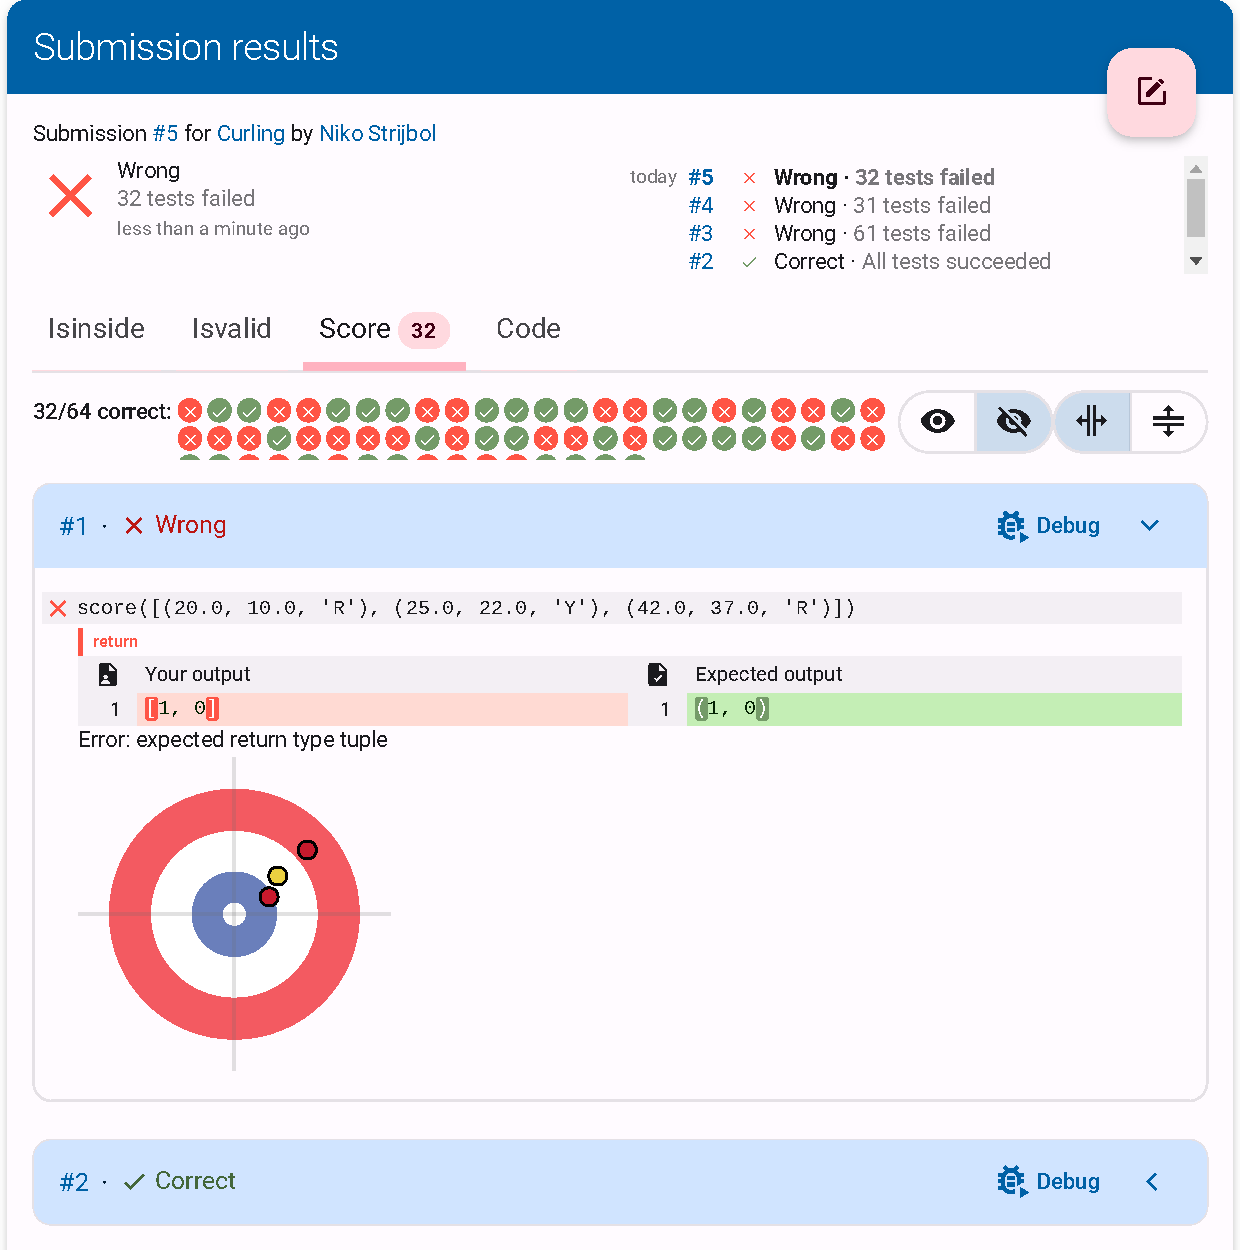
\includegraphics[width=\linewidth]{introduction/curling}
    \end{wide}
    \caption{
        An example of the feedback table for an incorrect Python submission for the exercise \textit{Curling} on Dodona.
        The feedback is split into three tabs (the fourth tab, ``Code'', contains the submission itself).
        As can be seen below the "Score" tab, only 32 of the 64 test cases are correct.
        The figure shows the first two test cases from the ``Score'' tab, the first of which is incorrect: the function should have returned a \texttt{tuple}, but returned a \texttt{list} instead.
        Besides showing the difference between the expected and actual value, Dodona also allows showing more information.
        In this case, a visual rendering of the curling position is given to aid students in debugging their code.
    }
    \label{fig:curling-feedback-table}
\end{figure}

One of the most important actionable components for both students and educators is the feedback table (\cref{fig:curling-feedback-table}).
This feedback table is flexible enough to accommodate a wide variety of feedback.
In the example, three types of feedback are illustrated: the difference between the expected and generated return value, a custom message, and an image.

As the feedback table shows custom data from an exercise or judge, which are not necessarily trusted, special attention has been paid to make the feedback table secure.
For example, all content is rigorously sanitized to prevent cross-site scripting attacks~\autocite{guptaCrossSiteScriptingXSS2017}.

\subsection{Exercises and content management}\label{subsec:exercises-and-content-management}

Dodona currently supports two types of ``learning activities'': programming exercises and reading activities.
A reading activity requires no submission, but students can mark them as read to confirm they did the reading.
Programming exercises allow students to submit code and receive feedback on their submissions.
However, the bar for what constitutes code can be low.
For example, Dodona has a Markdown judge, which generates a rendered (HTML) version of the Markdown code submitted by students, without automatically evaluating anything more than the validity of the Markdown.
Dodona can thus be used to collect plain text submissions from students.
Learning activities fully support internalization: Dodona currently supports Dutch and English.

Exercises in Dodona are managed in Git repositories.
A repository with a well-defined structure is usable as the source for exercises in Dodona.\footnote{\url{https://docs.dodona.be/en/references/repository-directory-structure/}}
This allows educators to be the owners of their exercises, in addition to all the other benefits of version control.
Every time an exercise is updated in the repository, Dodona will synchronize the exercises on the platform with the exercises in the repository.

Besides a test suite, which is needed for automated feedback, programming exercises also need a problem statement that specifies what students should do.
In Dodona, a problem statement is a Markdown or HTML file, in which educators have free rein to describe their exercise.
The programming exercise (including a problem statement and test suite), together with a judge (the Docker image and the testing framework) form a \emph{task package} as defined by \textcite{verhoeffProgrammingTaskPackages2008}.

\section{Structure of this dissertation}\label{sec:a-note-on-the-structure-of-this-thesis}

The main problem this dissertation addresses is the observation that there are shortcomings in existing educational tools for programming education.
Most of these shortcomings were first observed when using Dodona.
They can be split into five main research questions:

\begin{description}
    \item[RQ1] Can we design an educational software testing framework that supports automated assessment across programming languages based on a single test suite?
    \item[RQ2] What is the most ergonomic way to author programming exercises with support for automated assessment across programming languages?
    \item[RQ3] Can we design an educational software testing framework for the block-based programming language Scratch?
    \item[RQ4] Can we design an (educational) debugger for the block-based programming language Scratch?
    \item[RQ5] What common execution model for running and debugging Scratch code best optimizes both scenarios?
\end{description}

The first two questions relate to textual programming languages, while the last three questions are in the context of Scratch, a visual block-based language.
The reason for this split is that it became clear that the needs for textual and block-based programming languages are different enough to warrant a separate approach.

This split is reflected in the structure of this dissertation as well.
\Cref{part:tested} is about textual programming languages and consists of two chapters (\cref{ch:tested1,ch:tested-dsl}), which answer the first and second questions respectively.
\Cref{sec:intro-tested} gives an introduction to this first part.
\Cref{part:scratch} is about the block-based programming language Scratch.
The smaller \cref{ch:scratch-the-programming-environment} gives a short introduction to Scratch.
\Cref{ch:itch} addresses question three, while \cref{ch:blink} address the fourth question.
\Cref{ch:scratch-execution-model} then answers the fifth question.
\Cref{sec:the-second-part:-scratch} gives an introduction to this second part.

Finally, \cref{ch:conclusions-and-opportunities} summarizes the answers to the research questions and highlights some future opportunities.
Each chapter also contains its own conclusion where the details for that specific chapter are discussed.

The remainder of this chapter gives a high-level overview of each part: the context, motivation, and where applicable, our previous publications.
Similar to the conclusions, each chapter also has its own introduction, where the specifics for that chapter are introduced.

\section{Textual programming languages}\label{sec:intro-tested}

The first research question \requ{1} was inspired by the observation that using exercises and judges in Dodona required some manual work: ``Can we design a testing framework that supports automated assessment across programming languages with a single test suite?''.
A lot of programming exercises on Dodona seem usable in multiple programming languages, at least in concept.

Actually using an exercise in another programming language first requires a copy of the exercise to be made.
Then the existing test suite must be converted manually to the test suite format used by the judge for that particular programming language.
The other parts of the exercise (the configuration and task description) also need to be converted manually.
Additionally, since the exercises are copied, the exercises have to be kept in sync manually, or they risk diverging.

Implementing judges for different programming languages is also repetitive.
For each judge, a new test suite format has to be created, and all other tasks that a judge does (e.g.\ test scheduling, output handling) have to be re-implemented for each new judge.
Supporting a new feature also requires doing it for every judge, which often does not happen in practice.

\subsection{Programming-language-agnostic exercises}\label{subsec:programming-language-agnostic-testing}

The answer to the first research question \requ{1} is TESTed, an educational software testing framework we created.
Its defining feature is the ability to create programming-language-agnostic exercises.
This means that the same exercise (with one test suite) can be solved in multiple programming languages, with support for automated assessment.

TESTed is discussed in \cref{ch:tested1}, which is based on \textcite{strijbolTESTedEducationalTesting2023}.
\marginnote{A doctoral dissertation has no page limit, after all.}
Compared to the original publication, the chapter has been expanded with more information about the inner workings of TESTed, in addition to going more in-depth on technical aspects of the framework.

\subsection{Ergonomic authoring of exercises}\label{subsec:ergonomic-testing}

With a working prototype at hand, the second research question \requ{2} came rather naturally: ``What is the most ergonomic way to author exercises with support for automated assessment across programming languages?''.
We took a step back to look at what is required to go from a prototype to a viable option for creating programming exercises.
This analysis aimed to ensure the exercises could be used in educational practice, including high-stakes tests such as exams.
We want TESTed to be suitable for both educators in higher education and secondary education.
Our ambition was to make TESTed the default option for creating programming exercises in Dodona.

The result of this research is presented in a second publication: \textcite{strijbolTESTedDSLDomainspecificLanguage2024}.
It is included almost verbatim as \cref{ch:tested-dsl}.
By looking at (educational) software testing more broadly, we find two missing parts of the process of creating programming exercises.
The first missing and most important part is an ergonomic and approachable way of creating test suites for exercises.
Our solution is TESTed-DSL, a domain-specific language for authoring programming-language-agnostic exercises with support for automated assessment.
The second missing part is support for language-agnostic task descriptions.
We show that TESTed-DSL can also be used for task descriptions.

A new insight while working on TESTed-DSL was that TESTed is not only useful for creating programming-language-independent exercises, but is also suitable for exercises that are not intended to be used in multiple programming languages.
Therefore, we have taken special care to design TESTed-DSL to be useful for a wide audience of educators, including higher and secondary education.
For this reason, we also invested in our documentation, which contains reference documentation and a set of tutorials for commonly used exercise types.

\subsection{Organization of the first part}\label{subsec:organization-of-the-first-part}

\Cref{ch:tested1} discusses TESTed and \cref{ch:tested-dsl} discusses TESTed-DSL, both based on previous publications.
One consequence of this approach is that there is some overlap: for example, the introductions in both chapters broadly cover the same topic.
However, the focus of both is different enough that we feel there is no problem including both.
Another example of a consequence is the terminology used for the levels in the test suites (\cref{subsec:structure-of-a-test-suite,subsec:dsl-test-suite-structure}), which differs.
The first chapter uses the terminology as used by Dodona, while the second chapter changes the terminology in the domain-specific language to align more closely with the terminology used in the literature.
This illustrates the progressive insight that comes when working on a tool, and the interplay between the design stages and its application in practice.

Research on TESTed was started in 2019 as a master's thesis~\autocite{strijbolTESTedOneJudge2020}, as was TESTed-DSL in 2021~\autocite{selsTESTedProgrammeertaalonafhankelijkTesten2021}.

\subsection{Repositories and user documentation}\label{subsec:repositories-and-code}

As a software project, the source code for TESTed is important, if not more important than this dissertation.
Both TESTed and TESTed-DSL share the same repository, which is published under the \textsc{mit} licence.\footnote{\url{https://github.com/dodona-edu/universal-judge}}
Two sets of documentation are available, aimed at a different target audience:
\begin{itemize}
    \item The guides for educators wanting to create programming exercises.\footnote{\url{https://docs.dodona.be/en/guides/exercises/}}
    Most of these guides are currently only available in Dutch.
    \item The reference documentation, for a more in-depth look into more technical subjects.\footnote{\url{https://docs.dodona.be/en/references/tested/}}
    For example, this includes the documentation on how to extend TESTed to add support for additional programming languages.
\end{itemize}

\section{Block-based programming languages}\label{sec:the-second-part:-scratch}

For young students, learning to program is often done with specialized programming languages.
The most-used language in this context is Scratch, a visual block-based programming language~\autocite{resnickScratchProgrammingAll2009}.

Since Dodona is independent of any testing framework, we thus asked the third research question \requ{3}: ``Can we design an educational software testing framework for Scratch?''.
Our intention was to add support for Scratch to Dodona.

\subsection{Testing Scratch code}\label{subsec:testing-scrath-code}

The first prototype of Itch, our testing framework for Scratch, did just that: it added support for evaluating Scratch submissions in Dodona.
However, Scratch is not only a programming language, but a complete programming environment~\autocite{maloneyScratchProgrammingLanguage2010}.
We realized that properly supporting Scratch required accommodations that were too different from what Dodona could (or would) provide.
Additionally, while our group had experience with programming exercises for text-based languages, we had much less experience with Scratch in an educational context.

To address these issues, we sought an industrial and commercial partner.
We found this partner in CodeCosmos, the international brand of FTRPRF, which is an educational publisher that creates, among other things, teaching packs.
Schools can use these to fulfil their obligations as part of the move to introduce more computational thinking in secondary education.

The work was divided as follows: Ghent University was responsible for the technical aspects of the automated feedback for Scratch exercises, while CodeCosmos provided the lessons, the educational support, and last but not least, actual students to use the teaching packs.
Readers interested in knowing more might like to read an article about this collaboration in \textit{Dare To Think}, Ghent University's online magazine.\footnote{\url{https://www.durfdenken.be/en/research-and-society/coach-codi-boosting-tool-helps-children-become-independent-coders}}

The testing framework Itch, the answer to the third research question, is described in \cref{ch:itch}.
Itch allows both static and dynamic tests on Scratch exercises, which provides a lot of flexibility to educators.
Dynamic testing, in particular, allows for exercises that support (within limits) the exploratory nature of Scratch.

Itch test suites for Scratch exercises are written in JavaScript.
While working with CodeCosmos on creating Scratch exercises, it became clear that the JavaScript test suites were a big hurdle for educators without a computer science background.
As a lot of software testing frameworks are written in the same programming language as the code they test, we also explored this approach.
The result of this is Poke, a prototype of a testing framework for Scratch with test suites written in Scratch, discussed in \cref{sec:poke:-a-testing-framework-written-in-scratch}.
While technically feasible, there are still open questions regarding the practical use of this approach in an education setting.

\subsection{Debugging Scratch code}\label{subsec:debugging-scratch-code}

The goal of educational software testing and automated assessment is to provide students with feedback on their code.
However, the feedback in itself is not enough: we want students to be able to use that feedback and be able to correct their code if something went wrong.
The next step, after a failed test, is to debug the submission, which is a two-step process~\autocite{myersArtSoftwareTesting2012}.
Step one is determining the exact nature and location of the error, and step two is fixing said error.

It is well known that determining the cause of an observed failure is challenging~\autocite{ammannIntroductionSoftwareTesting2016}.
The debugging process is difficult, especially for novice programmers~\autocite{mccauleyDebuggingReviewLiterature2008}.
This has led to the creation of various tools to help with this, chief among them debuggers~\autocite{rosenbergHowDebuggersWork1996}.

This is also the case with text-based languages.
For example, this is why \cref{fig:curling-feedback-table} shows a ``Debug'' button in the feedback table of Dodona.
However, for Scratch, this area is much less developed.
The fourth research question \requ{4} thus became: ``Can we design a debugger for Scratch?''.

\Cref{ch:blink} discusses our answer to this question, in the form of Blink, our time-travelling debugger for Scratch.
A time-travelling debugger allows the programmer to go back in the execution, often by recording program execution~\autocite{barrTardisAffordableTimetravel2014,barrTimetravelDebuggingJavaScript2016,czaplickiAsynchronousFunctionalReactive2013,balzerEXDAMSExtendableDebugging1969,ungarDebuggingExperienceImmediacy1997,chenReversibleDebuggingUsing2001,crescenziReversibleExecutionVisualization2000}.
We took special care to make the debugger intuitive for the young target audience of Scratch.
Initial experiments in the classroom show that children do in fact find the debugger intuitive and useful, particularly stepping through the code and the time travel feature.

This chapter is a minimally modified copy of the publication \textcite{strijbolBlinkEducationalSoftware2024}.

\subsection{The Scratch execution model}\label{subsec:the-scratch-execution-model}

While working on the debugger, we also began looking more deeply into the Scratch execution model.
The Scratch execution model combines a fixed-step time loop (30 frames per second) with an almost-cooperative threading model.
This means that threads are seldom interrupted, mostly relying on explicit yielding to other threads.

This threading model was chosen because it minimizes the occurrence of some race conditions, although concurrency-related issues still occur~\autocite{maloneyScratchProgrammingLanguage2010}.
The cooperative nature of the threading model also has drawbacks: it can lead to unexpected behaviour when working with multiple sprites.

Additionally, the execution model also limits how a debugger can work, without resorting to deviating from the execution model as used during normal execution.

We thus asked ourselves, ``What execution model for running and debugging Scratch code best optimizes both?'' \requ{5}.
We investigate and answer this question in \cref{ch:scratch-execution-model}.
The chapter begins with a detailed look at how the current execution model behaves, followed by our proposed changes.
Since Scratch is so widely used, our changes should not negatively impact existing Scratch programs.
We therefore analyse what a typical Scratch project looks like.
Finally, we run some preliminary benchmarks with our proposed changes and report on the results.

While we initially set out to find \textit{the} replacement for the execution model, we no longer believe that a single replacement is possible.
Scratch programs, especially larger ones, rely on the current behaviour of the execution model, meaning any change to this behaviour would constitute a breaking change.
The proposed changes are still useful, but in more specialized contexts, instead of a general replacement.
For example, the proposed changes enhance the use of the debugger.
Smaller programs are much less affected by our proposed changes, and most programs are small.

\subsection{Organization of the second part}\label{subsec:organization-of-the-second-part}

The second part starts with \cref{ch:scratch-the-programming-environment}, which introduces Scratch, the programming language and environment.
Next, \cref{ch:itch} discusses Itch and Poke, our Scratch testing frameworks.
\Cref{ch:blink} then discusses Blink, our debugger for Scratch.
Finally, \cref{ch:scratch-execution-model} discusses the Scratch execution model, our proposed changes to it, an analysis of Scratch projects, and an evaluation of our proposed changes.

Work on these various tools for Scratch often began as a master thesis~\autocite{makItchEenEducatief2019,voetenEenBlokgebaseerdTestframework2023,goethalsEenTimeTravelling2023,deproftBlinkEenEducatieve2022,cattoireEenNieuwUitvoeringsmodel2024}.

\subsection{Repositories}\label{subsec:repositories-and-code-scratch}

The source code of Itch is not publicly available at this time due to the agreement with our partner CodeCosmos.
The source code for Blink is available under the same licence as Scratch, the \textsc{bsd} 3-Clause ``New'' or ``Revised'' Licence.\footnote{\url{https://github.com/scratch-ed/blink}}
We also host an online instance of the debugger.\footnote{\url{https://scratch.ugent.be/blink/}}

Our JavaScript implementation of an analysis tool for Scratch 3.0 (similar to Hairball; \cite{boeHairballLintinspiredStatic2013}) is available under the MIT Licence.\footnote{\url{https://github.com/scratch-ed/scratch-analysis}}

\part{\tested{}}\label{part:tested}
\chapter[An educational testing framework]{An educational testing framework with language-agnostic test suites for programming exercises}\label{ch:tested1}

\dictum[Attributed to Burt Rutan]{
    Testing leads to failure, and failure leads to understanding.
}

In educational contexts, automated assessment tools are commonly used to provide formative feedback on programming exercises.
However, designing exercises for automated assessment tools remains a laborious task or imposes limitations on the exercises.
Most automated assessment tools use either output comparison, where the generated output is compared against an expected output, or unit testing, where the tool has access to the code of the submission under test.
While output comparison has the advantage of being programming language independent, the testing capabilities are limited to the output.
Conversely, unit testing can generate more granular feedback, but is tightly coupled with the programming language of the submission.

In this chapter, we introduce TESTed, which enables the best of both worlds: combining the granular feedback of unit testing with the programming language independence of output comparison.
Educators can save time by designing exercises that can be used across programming languages.
We begin by giving a brief introduction and considering some related work.

We focus next on the technical aspects of TESTed, beginning with its architectural design.
Next, we consider the three parts of evaluating a submission:
the test suite, the evaluation process itself, and the generated feedback.

\marginnote{Note that TESTed now supports a user-friendlier test suite format: TESTed-DSL (\cref{ch:tested-dsl}).}
For the test suites, we discuss their structure, and look at how TESTed handles datatypes (across different programming languages), statements, and expressions.
Next, the evaluation process is discussed in detail.
This is the process through which TESTed executes the test suite and determines the feedback that will be given on the submission.
We also briefly look at the integration with Dodona.
This is relevant, as TESTed inherits some aspects from Dodona, such as the feedback format.
As a conclusion to the technical part, we discuss in detail how support for multiple programming languages is achieved.
We look at the internal API to give a good idea of what is required to support new programming languages.

Finally, we evaluate TESTed in educational practice.
We report on three quasi-experiments where we asked students to solve a set of programming exercises and automatically reviewed their submissions with TESTed.

\section{Introduction and background}\label{sec:tested1-introduction-and-background}

Formative feedback on solutions for programming exercises is a crucial part of learning to code~\autocite{shuteFocusFormativeFeedback2008,orrellFeedbackLearningAchievement2006,luxton-reillyIntroductoryProgrammingSystematic2018}.
Feedback is formative (and most valuable) if learners receive rich and qualitative feedback throughout the learning process~\autocite{blackDevelopingTheoryFormative2009}.
Providing such feedback by hand is a challenge for educators since it is a time-consuming activity~\autocite{camposMultinationalCaseStudy2012,cheangAutomatedGradingProgramming2003, keuningSystematicLiteratureReview2018,haoUnderstandingEffectiveDesign2021,zavalaUseSemanticbasedAIG2018,staubitzRepositoryOpenAutogradable2017,pirttinenCrowdsourcingProgrammingAssignments2018,gulwaniFeedbackGenerationPerformance2014,tangDatadrivenTestCase2016,edwardsDevelopingCommonFormat2008a}.
The challenge is further exacerbated by a large number of students who work on multiple exercises~\autocite{campGenerationCSGrowth2017,saxExaminingEnrollmentGrowth2017}.
Any laborious and time-consuming activity is a prime target for automation, and providing feedback is no different.
The computer science education field therefore has a long history of applying software testing frameworks or general-purpose software tools (linters, formatters, etc.) on source code to automatically generate feedback~\autocite{haoUnderstandingEffectiveDesign2021,edwardsUsingSoftwareTesting2004,paivaAutomatedAssessmentComputer2022,keuningSystematicLiteratureReview2018}.

Off-the-shelf tools such as linters are low effort for educators, but only provide generic feedback: there is no exercise-specific feedback.
Software testing frameworks require an accompanying test suite for each individual programming exercise, which means they require a lot more effort to create.
However, they can provide much more specific feedback.
A test suite typically contains a set of tests that verify if the submission satisfies the requirements in the task description of the exercise.
This is similar to the practice of unit tests or integration tests in the software engineering field.
Besides general testing frameworks, computer science education also uses judge systems~\autocite{paivaAutomatedAssessmentComputer2022,wasikSurveyOnlineJudge2018}: specialized learning environments that provide rich feedback.
Defining an adequate test suite for an exercise is part of the reason why creating programming exercises is so time-consuming~\autocite{zavalaUseSemanticbasedAIG2018,staubitzRepositoryOpenAutogradable2017,queirosPexilProgrammingExercises2011,pirttinenCrowdsourcingProgrammingAssignments2018,gulwaniFeedbackGenerationPerformance2014,tangDatadrivenTestCase2016}.

An apparent solution to reduce the amount of time needed to create programming exercises is to create fewer exercises.
To achieve this without reducing the number of exercises available to students, maximal reuse of existing exercises is necessary.
Existing solutions to facilitate reusing exercises include standard formats in which exercises are written~\autocite{paivaAnotherProgrammingExercises2020,verhoeffProgrammingTaskPackages2008}, open repositories with exercises~\autocite{staubitzRepositoryOpenAutogradable2017}, or tools to convert between existing exercise formats~\autocite{queirosBabeLOExtensibleConverter2013}.
However, reusing exercises remains difficult, particularly when attempting to reuse exercises across programming languages.
In most existing judge systems, exercises are tightly coupled to the programming language in which the test suite is written.
Alternatively, test suites without such tight coupling impose stringent restrictions on exercise specifications, for example only reading from standard input and writing to standard output.
Because of these restrictions, they often generate feedback of a lower quality than programming-language-specific test suites.

To reuse programming exercises written for another programming language, exercise designers first have to learn a new testing framework for that programming language.
Then, they have to write a new test suite for the exercise according to the specifications of the new testing framework.
Alternatively, due to the vast number of programming languages~\autocite{bissyandePopularityInteroperabilityImpact2013}, it might be necessary to implement a new testing framework to support educational software testing, which is no small undertaking.

We focus on facilitating easy reuse of programming exercises across programming languages.
Our contributions include defining requirements for a testing framework to support multiple programming languages, without imposing strict restrictions on programming exercises.
We also introduce TESTed, a proof-of-concept of a system that satisfies these requirements.
TESTed directly supports multiple programming languages for the same exercise, meaning the conversion of exercises to multiple testing frameworks is no longer needed.
Exercise designers working on exercises for a single programming language can also benefit from TESTed, as it no longer forces them to learn new testing frameworks for each new target language.
Finally, implementing support for new programming languages in TESTed is less work than implementing a complete testing framework for each language, reducing the software development and maintenance cost dramatically.

\section{Related work}\label{sec:tested1-related-work}

Since the terminology related to automated feedback on programming exercises is not used consistently within the field,
we begin by defining the terms used in this chapter.
A programming exercise is the combination of a \term{task description} and a \term{test suite}.
When students attempt to solve the exercise using the instructions from the task description, they create a \term{submission} for the exercise.
The test suite is used by a judge system to \term{evaluate} the submission.
This results in \term{feedback} that is shown to the student.

We consider it useful to split a judge system into a \term{judge platform} and a \term{testing framework}.
A judge platform is a graphical user interface that allows students and educators to upload and store submissions, display feedback, organize exercises into courses, and so on.
A testing framework is responsible for generating feedback, by executing and evaluating submissions based on a test suite.
In existing literature, the distinction between these two is not always made, nor is it always relevant.
For example, some review papers~\autocite{keuningSystematicLiteratureReview2018,wasikSurveyOnlineJudge2018} or individual tools~\autocite{bezURIOnlineJudge2014,petitJutgeOrgCharacteristics2018} consider the entire system as a whole.
Other papers focus specifically on judge platforms~\autocite{gusukumaPedalInfrastructureAutomated2020,strieweArchitectureModularGrading2016}.
However, we believe this distinction to be relevant, as evaluating submissions (the testing framework) has a separate set of challenges compared to judge platforms (for example, displaying feedback in a constructive way).
This chapter focuses on testing frameworks.

In educational contexts, software testing frameworks typically use either \term{output comparison} (also known as \term{input/output testing}) or \term{unit testing}~\autocite{paivaAutomatedAssessmentComputer2022} to evaluate submissions.
Programming language support of testing frameworks generally depends on the approach they adopt.
With unit testing, the test suite is often written in the same programming language as the submission, e.g.\ with tools based on xUnit~\autocite{meszarosXUnitTestPatterns2007}.
Since the test suite is often written in the same programming language as the submission, it has full access to the submission.
The test suite can use function calls, data structures (e.g.\ lists, maps), primitive data types (e.g.\ integers, strings), examine return values, exceptions, runtime inspections (e.g.\ reflection), etc.
As a result, the test suite is tightly coupled to a specific programming language.
Evaluating a submission for the same exercise in another programming language would require a new test suite, often also involving another testing framework.

With input/output testing, the judge system imposes stringent restrictions on the programming exercise: only standard input, standard output, standard error, and files can be used for input and output.
Prominent examples are the testing frameworks used in \textsc{icpc}-style (\emph{International Collegiate Programming Contest}, sometimes still referred to as ACM-ICPC)~\autocite{ICPCFactSheet2023} programming contests.
While this does make the test suites independent of any programming language, all aspects of the submission that the test suite needs to check must be converted to a textual representation.
Another disadvantage is the lack of granular testing: with these systems, tests are limited to the program as a whole.
It is, for example, not possible to add distinct tests for different functions inside the same program without obligating students to artificially split the program.

Wanting to support multiple programming languages is not new: \textcite{hextAutomaticGradingScheme1969} describe an early automated assessment system that supports multiple programming languages.
While it supports more than just input/output testing, it does not support a single test suite: every programming languages requires its own test code (the system was limited to two tests).
The reporting of the results was, however, unified across programming languages.

\section{Programming-language-agnostic testing frameworks}\label{sec:tested1-programming-language-agnostic-test-frameworks}

Intuitively, an ideal testing framework that supports multiple programming languages is a testing framework with the testing capabilities of unit testing and the programming language support of input/output testing.
First, we define the two requirements a framework needs to satisfy to achieve this.
We also look at the consequences of those requirements on the framework.
We call a testing framework that satisfies these requirements a \term{programming-language-agnostic testing framework}.

The \term{first requirement} is that test suites must be programming language agnostic.
A test suite must be usable to evaluate submissions in every programming language supported by the framework, without making changes to the test suite or adding languages-specific tests to it.
As a consequence of this requirement, adding support for new programming languages to the testing framework must not demand changes to existing test suites.
All existing test suites must work with the new programming language without changes.

The \term{second requirement} is that the framework must have testing capabilities similar to those of unit testing frameworks.
Some concrete examples of what should be possible are:

\begin{itemize}
    \item Using standard input, standard output, and standard error.
    \item Calling functions implemented in submissions, and passing arguments to those functions.
    \item Evaluating values returned from function calls (with data type support).
    \item Creating objects (constructors) and manipulating them (methods).
    \item Capturing and evaluating other side effects such as exceptions, exit codes or files (or other persistent storage such as databases).
    \item Supporting exercises with deterministic and non-deterministic (e.g.\ random) behaviour.
\end{itemize}

Support for these two requirements should not have disproportionately large drawbacks.
Therefore, we also consider the following soft requirements for a programming-language-agnostic testing framework:

\begin{itemize}
    \item Authoring exercises using the framework should not be significantly more difficult than authoring exercises using a language-specific testing framework.
    \item Runtime and memory overhead should be minimal: the framework cannot be unacceptably slow or have a large memory footprint compared to a language-specific testing framework.
    Providing feedback to students in a timely manner is important.
    \item Submissions should follow their language-specific conventions as closely as possible.
    For example, supporting asynchronous and synchronous functions in JavaScript, or top-level functions should be implemented as a static function in Java, but not in Python or Kotlin that have proper support for top-level functions.
    \item Adding support for new programming languages to the framework should ideally be faster than implementing language-specific testing frameworks for those languages, due to the ability to reuse shared parts of the implementation.
\end{itemize}

The next sections introduce TESTed, our implementation of such a framework.
We begin by showing an example of how TESTed is used, to give a good idea of what TESTed does.
Afterwards, the various parts of TESTed are discussed in detail.

\section{Using the framework}\label{sec:tested1-using-the-framework}

We start with a high-level tour of TESTed, focusing on how the framework can be used.
To this end, we will use the following programming exercise as an example:

\begin{quote}
    Implement a function \texttt{remove\_all\_occurrences} that takes two arguments: a list \textit{l} of integers and an integer \textit{v}.
    The function must return a new list containing the same integers as list \textit{l}, in the same order, but where all occurrences of integer \textit{v} are removed.
\end{quote}

A correct Python implementation for this exercise is:

\begin{minted}{python}
def remove_all_occurrences(l, v):
    return [x for x in l if x != v]
\end{minted}

A test suite for this exercise could contain a number of function calls with different arguments and check their return values against an expected value.
To keep things short, we limit ourselves here to a test suite with a single function call (\cref{lst:simple-json-test-suite}).

\begin{listing}
    \begin{minted}{json}
{
 "input": {
  "type": "function",
  "name": "remove_all_occurrences",
  "arguments": [
   {
    "type": "sequence",
    "data": [
     {"data": 1, "type": "integer"},
     {"data": 2, "type": "integer"},
     {"data": 3, "type": "integer"},
     {"data": 2, "type": "integer"}
    ]
   },
   {"data": 2, "type": "integer"}
  ]
 },
 "output": {
  "result": {
   "type": "sequence",
   "data": [
    {"data": 1, "type": "integer"},
    {"data": 3, "type": "integer"}
   ]
  }
 }
}
    \end{minted}
    \caption[]{
        Snippet of a JSON test suite with a single test case that calls the function \mintinline{python}{remove_all_occurrences} with two arguments:
        \begin{enumerate*}[label=\emph{\roman*})]
            \item a sequence containing the four integers 1, 2, 3 and 2,
            \item the integer 2.
        \end{enumerate*}
        The expected return value is a list containing the integers 1 and 3.
    }
    \label{lst:simple-json-test-suite}
\end{listing}

When evaluating a submission using this test suite, TESTed will first translate the test suite into the programming language of the submission.
Conceptually, each function call is converted into a test case:

\begin{minted}{python}
# Python
remove_all_occurrences([1, 2, 3, 2], 2) == [1, 3]
\end{minted}

\begin{minted}{javascript}
// JavaScript
removeAllOccurrences([1, 2, 3, 2], 2) === [1, 3]
\end{minted}

\begin{minted}{haskell}
-- Haskell
(removeAllOccurrences [1, 2, 3, 2] 2) == [1, 3]
\end{minted}

TESTed takes care of the differences between programming languages (syntax, default representations, and naming conventions).
The actual test code generated by TESTed is more complex, as it must capture return values, account for exceptions, etc.

\begin{figure}
    \centering
    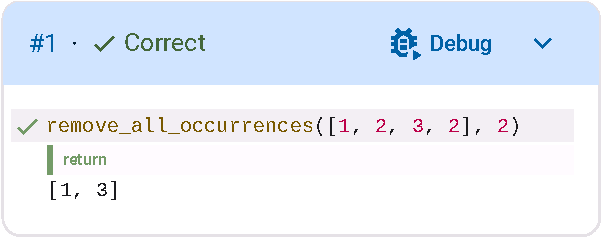
\includegraphics[width=0.5\linewidth]{tested-engine/dodona-rendering-small}
    \caption{An example of how the feedback for the test suite from \cref{lst:simple-json-test-suite} can be rendered (in this case, it is rendered by Dodona).}
    \label{fig:dodona-rendering-small}
\end{figure}

\begin{samepage}
    When TESTed evaluates the correct Python submission from before, it produces the following Python-specific feedback:

    \begin{minted}{json}
    {"command": "start-testcase"}
    {"description": "remove_all_occurrences([1, 2, 3, 2], 2)"}
    {"expected": "[1, 3]", "channel": "return"}
    {"generated": "[1, 3]", "status": "correct"}
    {"command": "close-testcase"}
    \end{minted}
\end{samepage}

A judge platform may then use this output to display a human-readable representation of the feedback (an example of this can be seen in \cref{fig:dodona-rendering-small}).
The feedback starts with a description of what has been tested (a function call in the programming language of the submission, in this case Python), followed by the expected return value and the actual return value (in a human-readable string representation).
With the actual return value, a decision is also given: in this case, the return value is correct.

While the output for correct submissions is important, the output for wrong submissions is at least as important in the context of an educational testing framework.
Assume a submission is wrong in that it only removes the first occurrence of the integer \textit{v} from the list \textit{l} (example in JavaScript):

\begin{minted}{javascript}
function removeAllOccurrences(l, v) {
  l.splice(l.indexOf(v), 1);
  return l;
}
\end{minted}

When TESTed evaluates this submission, its feedback reflects that while the code has been executed successfully, a logical error was found:

\begin{minted}{json}
{"description": "removeAllOccurrences([1, 2, 3, 2], 2)"}
{"expected": "[1, 3]", "channel": "return"}
{"generated": "[1, 3, 2]", "status": "wrong"}
\end{minted}

However, students sometimes do not even get to the point where their submission is executed successfully.
For example, they might submit a solution containing a syntax error (in Python):

\begin{minted}{json}
{"description": "remove_all_occurrences([1, 2, 2, 3], 2)"}
{"message": "Received compiler error:"}
{"message": "*** Error compiling..." }
{"status": "compilation error"}
\end{minted}

\marginnote{While Python is not considered a compiled language, it supports \texttt{python -m compileall}.}
Instead of an expected and actual return value, the feedback now contains the error message printed by the Python compiler.
If compilation fails, the submission will not be executed and testing is stopped.

\section{Architectural design of the framework}\label{sec:tested1-architectural-design}

\begin{figure}
    \centering
    \includestandalone{tested-engine/concept}
    \caption{
        Architectural design of TESTed, with colours indicating different programming languages.
        The framework consists of a set of Python packages and modules.
        These can be categorized as the core package and a set of programming-language-specific modules.
        The input for TESTed consists of a test suite, together with a submission in one of the supported programming languages.
        The output is the generated feedback.
    }
    \label{fig:conceptual-design}
\end{figure}

TESTed is built around the idea that an exercise author writes a single, unified test suite for the exercise, independent of any programming language.
TESTed then converts that test suite into the programming language of the submission on the fly, and takes care of the various aspects of the evaluation process: compiling the submitted code, executing the submission together with the test code, checking test results, and generating feedback.

While some parts of the evaluation process are programming-language-specific by necessity, such as generating the test code, a lot of the steps are not.
For example, creating an execution plan or interpreting the test results and generating the feedback are not specific to any one programming language.
Therefore, the language-specific aspects are isolated in language modules, as illustrated in \cref{fig:conceptual-design}.

\leavevmode\marginnote{
    A Python module is a \texttt{.py} file, while a Python package is a folder containing modules.
}%
TESTed is written in Python and organized into a set of Python modules and packages.
An import package is the \emph{core} package, which contains modules that are responsible for all language-agnostic tasks, such as scheduling tests.
We provide an in-depth description of the full evaluating process in \cref{subsec:execution-planning}.
In most cases, the core is also responsible for checking the collected test results and generating the feedback.
This is discussed in \cref{subsec:checking-results}.

All aspects that are specific to one programming language are bundled in one package.
These language-specific modules take care of all language-specific tasks, such as compiling submissions, executing submissions, and handling language-specific data types, expressions, and statements.
Since the language-specific code is limited to these modules, this offers benefits for adding support for new programming languages to TESTed, as discussed in \cref{sec:programming-language-support}.

TESTed takes as input the test suite for a programming exercise and a possible submission that needs to be evaluated.
The format of the test suite is discussed in-depth in \cref{sec:test-suites}.
As a result of its evaluation, TESTed outputs a feedback report (\cref{sec:tested-and-dodona})

\section{Test suites}\label{sec:test-suites}

Despite multiple proposals on generic formats for programming exercises~\autocite{edwardsDevelopingCommonFormat2008a,paivaAnotherProgrammingExercises2020,queirosPexilProgrammingExercises2011,verhoeffProgrammingTaskPackages2008} or exercise classifications~\autocite{leOperationalizingContinuumWelldefined2013,simoesNatureProgrammingExercises2020}, there seems to be no generally accepted standard for test suites of programming exercises.
Additionally, none of the proposed formats meets the requirements that we identified for language-agnostic testing frameworks.
Existing formats focus mostly on the task description, whereas we mainly focus on the specification of the test suite itself.

We therefore feel it is appropriate to introduce a new format for test suites, specifically developed for TESTed.
It is designed to be machine and human-readable and easy to generate.
Making it ergonomic to write by hand was only a secondary goal.
While the format is not framework-specific, and could thus be adopted by other testing frameworks, this was not an explicit design goal.

Test suites for TESTed are written in JSON, which was chosen because there is broad support in programming languages.
Additionally, it is human-editable and readable, especially compared to binary formats.
There is also widespread editor support for JSON, and technologies such as JSON Schema allow for easy validation and even better editor support.

Note that TESTed-DSL (\cref{ch:tested-dsl}) is the intended way to author exercises, especially if done manually.
The test suites discussed here are a direct JSON representation of the internal structure of test suites as used by TESTed, and thus much more verbose and not guaranteed to stay stable in future version of TESTed.

\subsection{Structure of a test suite}\label{subsec:structure-of-a-test-suite}

Returning to the same programming exercise from before, we can expand the test suite of \cref{lst:simple-json-test-suite} for illustration purposes (resulting in \cref{lst:expanded-json-fragment}, rendered in \cref{fig:dodona}).
Instead of directly calling the function \mintinline{python}{remove_all_occurrences} with two arguments, we first create a list and assign it to a variable in the first test case.
In the second test case, we then call the function \mintinline{python}{remove_all_occurrences}, but use the variable name as the first argument.

While omitted for brevity in the examples, a test suite can organize test cases in two levels: tabs and contexts.
The full hierarchy of the test suite consists of four levels, from top to bottom:

\begin{enumerate}[noitemsep]
    \item \term{Tabs} are the top-level grouping mechanism.
    It allows logically grouping contexts together.
    While the name of this group suggests how to display these groups, it is but a suggestion.
    The example only has one tab, but a test suite with test cases for multiple functions might, for example, have one tab per function.
    \item \term{Contexts} are meant to group dependent test cases together.
    In our example, declaring a variable and using that variable must be done within the same context.
    \item \term{Test cases} are the basic building blocks of the test suite.
    The ``input'' for a test case is what exactly is being checked.
    In the example, the first test case of each context has an assignment, while the second has a function call.
    \item \term{Tests} are used for each type of output.
    TESTed currently supports return values, standard output, standard error, exceptions, generated files and exit codes.
    In the example there is one test for the return value.
    If a test is not defined (e.g.\ for standard error in the example), a sensible default is used.
    For example, the default test for standard output and error checks that there is no output, causing the evaluation to fail if there is unexpected output.
\end{enumerate}

\begin{listing}
    \begin{minted}{json}
{
 "variable": "a_list",
 "type": "sequence",
 "expression": {
  "type": "sequence",
  "data": [
   {"data": 1, "type": "integer"},
   {"data": 2, "type": "integer"},
   {"data": 3, "type": "integer"},
   {"data": 2, "type": "integer"}
  ]
 }
}, {
 "input": {
  "type": "function",
  "name": "remove_all_occurrences",
  "arguments": [
   "a_list",
   {"data": 2, "type": "integer"}
  ]
 },
 "output": {
  "result": {
   "value": {
    "type": "sequence",
    "data": [
     {"data": 1, "type": "integer"},
     {"data": 3, "type": "integer"}
    ]
   }
  }
 }
}
    \end{minted}
    \caption[]{
        A snippet of a JSON test suite for TESTed with two statements:
        \begin{enumerate*}[label=\emph{\roman*})]
            \item declaration of a variable (\texttt{a\_list}) that is assigned a sequence containing four integers 1, 2, 3, and 2 and
            \item call of the function \texttt{remove\_all\_occurrences} with two arguments: \texttt{aList} and the integer 2.
        \end{enumerate*}
        The expected return value is a list containing the integers 1 and 3.
        A potential way to render this feedback resulting form this test suite is shown in \cref{fig:dodona}.
    }
    \label{lst:expanded-json-fragment}
\end{listing}

\begin{figure}
    \centering
    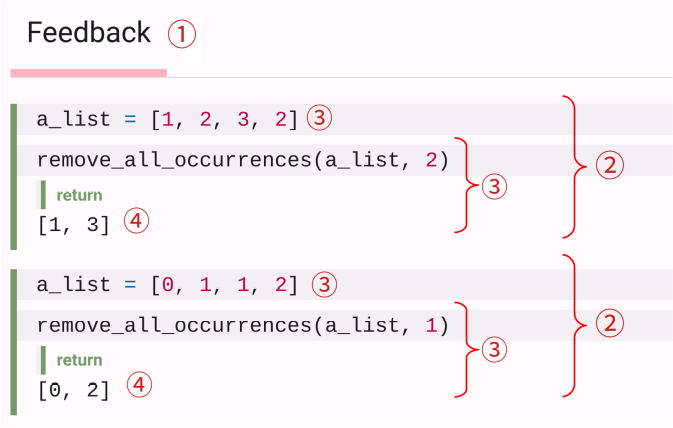
\includegraphics[width=0.6\textwidth]{tested-engine/dodona-rendering}
    \caption{A way to visually render the feedback (as done in Dodona) resulting from evaluating a submission (in Python) with the test suite from \cref{lst:expanded-json-fragment}.
    There are four levels: \CircledText{1} tabs, \CircledText{2} contexts, \CircledText{3} test cases, and \CircledText{4} the tests.
    Here, each context consists of two test cases, the first of which has no explicit tests, while the second has one explicit test (the expected return value).}
    \label{fig:dodona}
\end{figure}

This structure mirrors the output generated by TESTed (\cref{sec:tested-and-dodona}).
For example, the executed input for each test is also included in the output.
A possible visualization of these levels is given in \cref{fig:dodona}, which shows the output rendered in Dodona~\autocite{vanpetegemDodonaLearnCode2023}.

\subsection{Data serialization}\label{subsec:data-serialization}

TESTed uses data serialization to convert between the language-agnostic format of the test suite, and the generated test code.
Additionally, the same data serialization is used to convert return values from the submission into the language-agnostic format for checking (as described in \cref{subsec:checking-results}).

\begin{table}
    \caption{
        Overview of the basic types of TESTed and their implementation in the programming languages currently supported by TESTed.
        Sometimes, another type is used instead, based on the value. For example, an integer that is too large for \texttt{int} in Java will become a \texttt{long}.
        A dash (-) is used to indicate that the programming language does not support this type.
    }
    \label{tab:tested-basic-types}
    \begin{wide}
        \small\setlength{\tabcolsep}{0.5\tabcolsep}%
        \begin{tabular}{|l|l|l|l|l|l|l|l|l|}
            \hline
            \tested{} & Python         & JavaScript       & Java             & Kotlin           & Haskell          & C               & Bash          & C\#                 \\
            \hline
            integer   & \texttt{int}   & \texttt{Number}  & \texttt{int}     & \texttt{Int}     & \texttt{Int}     & \texttt{int}    & -             & \texttt{Int32}      \\
            real      & \texttt{float} & \texttt{Number}  & \texttt{double}  & \texttt{Double}  & \texttt{Double}  & \texttt{double} & -             & \texttt{Double}     \\
            boolean   & \texttt{bool}  & \texttt{Boolean} & \texttt{boolean} & \texttt{Boolean} & \texttt{Bool}    & \texttt{bool}   & -             & \texttt{Boolean}    \\
            text      & \texttt{str}   & \texttt{String}  & \texttt{String}  & \texttt{String}  & \texttt{String}  & \texttt{char*}  & \texttt{text} & \texttt{string}     \\
            sequence  & \texttt{list}  & \texttt{Array}   & \texttt{List}    & \texttt{List}    & \texttt{{[}{]}}  & -               & -             & \texttt{List}       \\
            set       & \texttt{set}   & \texttt{Set}     & \texttt{Set}     & \texttt{Set}     & -                & -               & -             & \texttt{Set}        \\
            map       & \texttt{dict}  & \texttt{Object}  & \texttt{Map}     & \texttt{Map}     & -                & -               & -             & \texttt{Dictionary} \\
            nothing   & \texttt{None}  & \texttt{null}    & \texttt{null}    & \texttt{null}    & \texttt{Nothing} & \texttt{void}   & -             & \texttt{void}       \\
            \hline
        \end{tabular}
    \end{wide}
\end{table}

Each literal value is described by an object with two attributes: a value (e.g.\ the number \texttt{5.3}) and a data type (e.g.\ \texttt{real}).
These attributes are combined into a JSON object with two fields.
The value is encoded using the closest representation available in JSON\@.
For example, a number is represented by a JSON number, and a string is represented by a JSON string.
The data type of a literal value is more complex, since TESTed targets multiple programming languages that each support their own collection of data types.
TESTed therefore defines a set of rules to denote data types and their support in programming languages.
This allows TESTed to convert types between programming languages.

TESTed uses two categories of data types.
The first category is a limited set of \term{basic types} that are abstract and map to concepts.
Currently, the following basic types are supported:

\begin{description}[noitemsep]
    \item[\texttt{integer}] An integer.
    The size of the integer is left undefined.
    \item[\texttt{real}] A real number.
    The size and precision of the real is left undefined.
    \item[\texttt{boolean}] A Boolean value.
    \item[\texttt{text}] Textual data (e.g.\ strings).
    The intention is important here: for example, an ASCII character can be represented as both an integer or as text.
    \item[\texttt{sequence}] An ordered sequence of values.
    \item[\texttt{set}] An unordered collection of unique values.
    \item[\texttt{map}] A collection of key-value pairs, where the keys are unique.
    \item[\texttt{nothing}] A representation of ``nothing'', meaning no value.
    \item[\texttt{any}] Any or unknown data type.
    This type is not usable in test suites, but is used to indicated return values of an unknown type.
\end{description}

When a test suite contains a literal value of a basic type, it will be serialized as an object of an actual data type in the target programming language.
An overview of all basic types and their implementation is given in \cref{tab:tested-basic-types}.
For example, a literal value with data type \texttt{map} will become a \texttt{Map} in Java and a \texttt{dict} in Python.

The second category consists of \term{advanced types}, which are more detailed or programming language specific.
Each advanced type is associated with a basic type, acting as a fallback.
For example, \texttt{int64} is an advanced type with the basic type \texttt{integer} as a fallback.
If a programming language does not support a particular advanced type, the corresponding basic type will be used.
For example, consider tuples.
Many programming languages do not have direct support for tuples, but exercises using tuples can still be solved by using the corresponding basic type (sequence).
More concrete, an exercise using the advanced type \texttt{tuple} can be solved in Java by using a \texttt{List}.

When adding a programming language, it is possible to disable this fallback for certain types.
For example, JavaScript has no support for fixed precision numbers.
This prevents TESTed from evaluating submissions in JavaScript if fixed precision numbers are used in the test suite.
TESTed will generate an appropriate error in this case.

Currently supported advanced types are:

\begin{description}[noitemsep]
    \item[\texttt{int8}] 8-bit integers (signed)
    \item[\texttt{uint8}] 8-bit natural numbers (unsigned)
    \item[\texttt{int16}] 16-bit integers (signed)
    \item[\texttt{uint16}] 16-bit natural numbers (unsigned)
    \item[\texttt{int32}] 32-bit integers (signed)
    \item[\texttt{uint32}] 32-bit natural numbers (unsigned)
    \item[\texttt{int64}] 64-bit integers (signed)
    \item[\texttt{uint64}] 64-bit natural numbers (unsigned)
    \item[\texttt{bigint}] integers without upper and lower limit (signed)
    \item[\texttt{single\_precision}] single precision real number
    \marginnote{The names for real numbers are borrowed from IEEE 754.}
    \item[\texttt{double\_precision}] double precision real number
    \item[\texttt{double\_extended}] double extended precision real number
    \item[\texttt{fixed\_precision}] fixed precision real number
    \item[\texttt{array}] a mutable fixed-size sequence
    \item[\texttt{list}] a mutable variable-size sequence
    \item[\texttt{tuple}] an immutable sequence
    \item[\texttt{char}] a single character
    \item[\texttt{undefined}] \texttt{undefined} in JavaScript
    \item[\texttt{null}] \texttt{null} in JavaScript
\end{description}

The advanced data types are also where the language-specific aspects can come into play.
For example, in addition to the basic type \texttt{nothing}, we have both \texttt{undefined} and \texttt{null}.
In most languages, there is no difference between those, but for example, in JavaScript there is.
Having both available as an advanced type allows exercises to use either in JavaScript exercises, while still being language-agnostic.
Additionally, supporting both types allows for the creating of language-specific exercises for JavaScript, where one of the types is required but not

\subsection{Statements and expressions}\label{subsec:tested1-statements-and-expressions}

We return once more to the test suite from \cref{lst:simple-json-test-suite}, which evaluates a function call.
It illustrates the need for TESTed to support a language-agnostic description of expressions and statements.
Evaluation of an expression yields a value, where TESTed allows describing expected values as identifiers (referring to a variable that was previously defined), function calls or literal values (using the data serialization format described in the previous section).
A statement in TESTed is either an assignment (defining a new variable) or an expression (similarly to Python: every expression is also a statement in its own right).

Note the absence of control structures or operators in the description of expressions and statements.
Our goal is not to create a full-fledged abstract programming language.
We intentionally limit expressions and statements to features needed by TESTed.
Creating a universal programming language that can be converted to all other programming languages is out of scope.

The use of assignments is illustrated by the expanded test suite in \cref{lst:expanded-json-fragment}.
We create a list and assign it to the variable \texttt{a\_list}.
Note that there are no explicit tests in this first test case.
The test case will still fail if something unexpected happens, e.g.\ if an exception is thrown or output is written to standard error.
The second test case then calls the function but uses the variable we defined as the first argument.

\section{Evaluating submissions}\label{sec:tested1-evaluating-submissions}

This section discusses the complete process through which a submission is evaluated.
The input for the evaluation process is a test suite and a submission, which is typically provided by the judge platform in which TESTed runs (or can be provided manually if TESTed is run on the command line).
Subsequent subsections dive into more detail of individual parts of the process.

\Cref{fig:flow} is a schematic overview of said evaluation process.
Step zero in the evaluation process is checking if the exercise is solvable in the programming language of the submission (\cref{subsec:solvability-and-correctness-checks}).
Next, the test suite is partitioned into compilation and execution units (\cref{subsec:execution-planning}).
For each of these units, the relevant test code is generated and compiled (\cref{subsec:code-generation}), in the programming language of the submission.
This code generation is the bulk of language-specific code in TESTed, whose design and implementation are discussed in \cref{sec:programming-language-support}.

After compilation, each resulting executable contains one or more execution units.
These are then all executed, and the side effects (such as exceptions, standard output, standard error) and results (i.e.\ return values) are recorded (\cref{subsec:executing-test-code}).
These results are then checked for correctness against the test suite (\cref{subsec:checking-results}).
This results in the feedback, which is returned by TESTed.

TESTed also provides an opportunity for static analysis on the submission.
\marginnote{Examples include \software{ESLint}, \software{Pylint}, and \software{HLint}.}
Currently, all supported programming languages run a linter on the submission, the results of which are also included in the feedback as code annotations (\cref{subsec:static-analysis-of-the-submission}).

\begin{figure}
    \centering
    \includestandalone{tested-engine/flow}
    \caption{
        The process of evaluating a submission in TESTed.
        TESTed is typically run within a judge platform, which provides the submission, the test suite and the configuration options.
        The contexts in the test suite are organized into compilation units and then execution units.
        For each compilation unit, the test code is generated, which is then compiled.
        The execution units are then executed, which yields execution results. These are then checked, resulting in feedback.
        Separately, a linter performs static analysis on the code quality of the submission, and the resulting output is also included in the feedback.
    }
    \label{fig:flow}
\end{figure}

\subsection{Correctness and solvability checks}\label{subsec:solvability-and-correctness-checks}

The first step in the evaluation process is checking if the test suite is usable for the programming language of the submission.
This might not be the case for a number of reasons, the three main ones being:

\begin{itemize}
    \item The exercise author has explicitly limited in which programming languages the exercise may be solved.
    \item The test suite uses constructs that are not supported by the programming language of the solution.
    For example, if the test suite uses object-oriented programming, the exercise will not be solvable in C or Haskell.
    \item The test suite contains programming-language-specific code but does not provide code for the programming language of the submission.
    For example, if a language-specific expression is only provided for Python, the exercise will only be solvable in Python.
\end{itemize}

Additionally, there are some correctness checks.
For example, the structure of the test suite is checked with JSON Schema.
TESTed takes a fail-fast approach~\autocite{shoreFailFastSoftware2004}: instead of silently failing when a test suite contains an error, TESTed will always abort the evaluation with an error message.

\subsection{Execution planning}\label{subsec:execution-planning}

The next step is planning the execution of the evaluation: creating an execution plan.
As discussed before, a test suite contains a number of contexts, which must be independent of each other.
TESTed partitions these into \term{compilation units} (a set of contexts that are compiled together), which are in turn partitioned into \term{execution units} (a set of contexts that are executed together).
This partitioning is what we consider the execution plan.

If performance was not a consideration, the simplest execution plan would be to compile and execute every context individually.
After all, contexts are independent of each other, and separate compilation and execution would enforce that independence.
However, this would be prohibitively slow: a test suite with fifty contexts would need fifty compilation steps and fifty execution steps.
Creating an execution plan is thus necessary to improve performance, which is achieved by reducing the number of compilation units and execution units.

\begin{figure}
    \begin{subfigure}{\textwidth}
        \centering
        \includestandalone{tested-engine/planning-1}
        \caption{
            A schematic representation of a test suite, with three tabs and eight contexts.
            The tabs are represented with green boxes, while the contexts (denoted as C\textsubscript{$n$}) are black boxes.
        }
        \label{fig:planning-suite}
    \end{subfigure}
    \par\bigskip
    \begin{subfigure}{\textwidth}
        \centering
        \includestandalone{tested-engine/planning-2}
        \caption{
            The two possible partitionings for compilation units (which are denoted by red boxes).
            The upper partitioning consists of a single compilation unit for the whole test suite.
            This is always tried first.
            If this fails, each tab becomes its own compilation unit (the red boxes thus overlap with the green ones).
        }
        \label{fig:planning-compilation}
    \end{subfigure}
    \par\bigskip
    \begin{subfigure}{\textwidth}
        \centering
        \includestandalone{tested-engine/planning-3}
        \caption{
            Two possible partitionings for execution units (denoted by blue boxes), depending on the partitioning of the compilation units.
            In the first partitioning (top), the single compilation unit is split into three execution units.
            The second partitioning (bottom) cannot use the same execution units, as an execution unit cannot comprise multiple compilation units.
            The compilation units are thus further divided into more execution units.
        }
        \label{fig:planning-execution}
    \end{subfigure}
    \caption{Schematic representation of the planning steps.}
\end{figure}

\subsubsection{Compilation units}
\label{subsubsec:compilation-units}

First, TESTed tries to use a single compilation unit for the whole test suite.
This is achieved by creating a program that accepts an argument to indicate which execution should be run.
In programming languages without an explicit compilation step, the compilation is no more than a syntax check.
\marginnote{
    For example, our JavaScript implementation uses \texttt{node -c}.
}
In compiled languages, the compilation is often much stricter, for example, failing if a non-existing function is used.

Techniques used to improve performance must be weighed against the usefulness of the generated feedback.
For example, consider an exercise where students must implement two functions (functions A and B).
Students might submit a solution in which they only implement function A\@.
With a single compilation unit, the generated test code contains calls to both function A and B\@.
This will this result in a compilation error, as a call to a non-existing function is not allowed.
This will prevent function A from being evaluated, even if it was correct.

To prevent this, if the compilation of the whole test suite fails, TESTed falls back to using one compilation unit per tab in the test suite.
These two approaches are illustrated in \cref{fig:planning-compilation}.
This is why a tab is intended to be a set of logically related contexts.
Continuing with the example from before, there might be a separate tab A for tests involving function A and a second tab for tests involving function B\@.
Going more fine-grained, by compiling each context individually, does not seem useful.
While potentially providing better feedback, the performance impact is significant.
Compiling at the tab level is a good compromise between fine-grained compilation (thus allowing more of the submission to be evaluated) and performance (the more compilation units, the slower the evaluation will be).

\subsubsection{Execution units}

Next, the compilation units from the previous steps are partitioned into execution units.
\marginnote{
    All programming languages, including the non-compiled ones, are handled the same way.
    This allows the most consistency between programming languages.
}
Each execution unit can be at most one compilation unit: we cannot execute multiple compilation units together,
as each compilation unit results in a separate executable.
However, depending on the contexts inside a compilation unit, we can (and do) execute a compilation unit multiple times.

For performance reasons, the ideal partitioning would be a single execution unit for the whole test suite.
However, this prevents certain types of exercises from being evaluated correctly.
Therefore, a new execution unit is started based on the type of context: if a context has standard input, command line arguments, or an explicit check for the exit code, a new execution unit is started.

\subsection{Generating test code}\label{subsec:code-generation}

Depending on the execution plan, the appropriate code is generated for the test suite.
In concept, this step converts the language-agnostic test suite into actual source code, in the programming language of the test suite (an example of this is shown in \cref{sec:tested1-using-the-framework}).
For example, a submission in JavaScript requires generating code in JavaScript.

Code is generated for each compilation unit.
The main purpose of the generated code is to execute the tests specified in the test suite.
For this reason, we also call the generated code the \term{test code}.
Besides executing the tests from the test suite, the generated code also contains some ceremonial code required by TESTed.
Some examples of this ceremonial code are:

\begin{itemize}
    \item As a compilation unit can contain multiple execution units, we generate a wrapper that executes the correct execution unit based on some parameter (e.g.\ \texttt{./testcode "unit1"}).
    \item The generated code includes serialization capabilities (\cref{subsec:data-serialization}), to convert captured values into the internal data format used by TESTed.
    \item The tests are wrapped in code that captures side effects and values, such as exceptions, return values, etc.
\end{itemize}

This code generation is the main task of the programming-language-specific modules, discussed in \cref{sec:programming-language-support}.

\subsection{Executing test code}\label{subsec:executing-test-code}

After the test code has been generated and compiled into executables, these executables are then executed.

During this execution, special care is taken to ensure that the executions are independent of each other.
All execution takes place in a special directory called the \emph{workdir} (from working directory), whose location is provided to TESTed via the configuration (\cref{sec:tested-and-dodona}).
For each execution unit, TESTed creates a new subdirectory and copies the relevant files into that subdirectory.
The execution then happens in the subdirectory.

Since an execution unit consists of one or more independent contexts, they are also independent of each other.
Another performance benefit of this independence is that this allows parallel execution of the different execution units.
Of course, this is only relevant if there are multiple execution units, but this is the case with most exercises in our experience.

Another benefit is better feedback.
Since TESTed copies all files into a dedicated subdirectory for each execution unit, we reduce chances of executions interfering with each other.
For example, consider an erroneous submission for an exercise where data is provided in a file.
If the submission overwrites or changes the file by accident, subsequent executions would use the modified file.

The astute reader might wonder how parallel execution is implemented, since TESTed is written in Python, a language whose default implementation (\software{CPython}) has an infamous global interpreter lock (GIL).
\marginnote{
    Work is ongoing to remove the GIL from \software{CPython}, as PEP 703.
}
This means that at any one time, only one thread can execute Python code.
However, TESTed executes the test code in a separate process.
This means the global interpreter lock does not apply: during execution of the test code, most of the time is spent waiting on results from the subprocess that is actually doing the execution.
Waiting on input/output results is one area where the global interpreter lock is released, even in current Python versions.

\subsection{Checking test results}\label{subsec:checking-results}

The code responsible for checking whether test results (return values, standard output, etc.) are correct is called an oracle~\autocite{howdenTheoreticalEmpiricalStudies1978}.
TESTed supports three types of oracles, which can be divided into two categories: language-agnostic oracles that work for all programming languages and language-specific oracles, where each programming language requires a separate implementation of the oracle.
Language-agnostic oracles are further divided into built-in oracles and programmed oracles.

The built-in oracles are provided by and included in TESTed.
These are rather simple, but should nevertheless suffice for most exercises.
We envision that as a natural evolution of using TESTed more broadly, other generic comparison methods might present themselves for inclusion in the framework.
Currently, the following oracles are included:

\begin{description}
    \item[Text oracle] This oracle compares two strings and is used for standard output and standard error.
    The oracle has some options, for example, to ignore trailing whitespace, to attempt to parse the text as floating point numbers or case sensitivity.
    The expected value can be provided either as a string, or as a file, in which case the contents of said file are used as the string.
    \item[File oracle] This allows comparison between two files, either comparing the whole file, or comparing the file line-by-line.
    When comparing line-by-line, the text oracle is used, so the same options can be provided.
    \item[Return value oracle] This oracle compares two values (using the serialization from \cref{subsec:data-serialization}).
    The oracle uses the basic and advanced types of TESTed to compare the data types in addition to the values.
    \item[Exception oracle] This allows checking exceptions.
    By default, only the message of the exception is checked, as the type of an exception is programming language dependent.
    However, the oracle does have an option to provide the expected type for the different programming languages.
    Do note that checking the type happens with a string-based check, meaning that if a student implements a custom exception with the same name, it will pass the check.
\end{description}

There are a number of scenarios where the built-in oracles are not enough to properly check an exercise.
One such example is an exercise where dynamic data is used, for example a return value that depends on the current date.
Another example is a random or otherwise non-deterministic return value, where the value must satisfy some conditions.
Finally, sometimes the exercise is static, but it is better to provide some exercise-specific feedback.
For example, if the exercise is to generate an SVG, it would be better to include a rendered version of the SVG in the feedback.

For these scenarios, a programmed oracle can be used.
\marginnote{Earlier versions of TESTed allowed implementing programmed oracles in any of the supported programming languages. Because of serious performance penalties, this is no longer allowed.}
Such an oracle is, in essence, an extension of the built-in oracles: instead of using a built-in oracle, TESTed will call the exercise-provided oracle.
Exercise authors must provide the oracle in the form of a function (the check function) implemented in Python.
This oracle is also language-agnostic: the same check function will be used for all programming languages.

Lastly, there are the language-specific oracles, which are provided as an escape hatch.
These oracles are run together with the generated test code and skip the data serialization pipeline.
They are therefore not subject to the serialization limits of TESTed.
An example of a scenario where this could be useful is an exercise where a function returns an instance of a custom class or any built-in datatype that does not map to a TESTed datatype.

The big downside to using these oracles is that they are programming language specific.
The oracle thus has to be implemented in each programming language the exercise supports.
These oracles are therefore only provided as an escape route for language-specific expressions, statements, and data types.
We discourage their usage as much as possible.

\subsection{Static analysis of the submission}\label{subsec:static-analysis-of-the-submission}

TESTed also provides a way to perform exercise-independent static analysis on the submission as part of the evaluation process.
The use of linters is widespread in the software engineering world and can also benefit students by pointing to common errors and familiarize students with the programming style of the language they are working in~\autocite{alomarUseStaticAnalysis2023}.
Currently, all supported languages (except C\#, where the compiler acts a linter) in TESTed use an external linter to generate additional feedback (\cref{tab:linters}).

\begin{table}[h]
    \centering
    \caption{
        Overview of the linters used by TESTed.
        For C\#, the compiler already provides linter-style warnings and feedback.
    }
    \label{tab:linters}
    \begin{tabular}{|l|l|}
        \hline
        Programming language & Linter \\
        \hline
        Bash & Shellcheck  \\
        C & Cppcheck \\
        C\# & (compiler) \\
        Haskell & HLint \\
        Java & Checkstyle \\
        JavaScript & ESLint \\
        Kotlin & Ktlint \\
        Python & Pylint \\
        \hline
    \end{tabular}
\end{table}

\section{Integration with and influences of Dodona}\label{sec:tested-and-dodona}

Dodona~\autocite{vanpetegemDodonaLearnCode2023} is an online platform for solving and submitting programming exercises.
An introduction and overview of the platform is given in \cref{sec:dodona}.
Relevant here is the distinction between a judge platform and testing framework (\cref{sec:tested1-related-work}): Dodona is the judge platform in which different testing frameworks (the judges in Dodona terminology) can be run.

While TESTed is available as a standalone tool, it was primarily developed with Dodona in mind.
Therefore, some design decisions made by the Dodona platform still apply to TESTed as well.
In this section, we briefly discuss the relevant aspects of Dodona that have an impact on TESTed.
We also look at Dodona's feedback format, which is also used by TESTed.

\subsection{Architecture of the Dodona platform}\label{subsec:dodona-architecture}

Dodona enforces a complete separation of the platform code and the testing framework.
Communication between the platform and the testing frameworks is done via a well-defined interface, consisting of two parts: the input for testing frameworks and the feedback generated by testing frameworks.
Both are discussed in the next two sections.
Evaluating submissions is done using \software{Docker}, as testing frameworks run student code.
They must be immune to bad code, e.g.\ a submission with an infinite loop should not bring down the platform.
Neither should malevolent submissions: a fork bomb should similarly have no impact on the platform.

When code is submitted, the platform will create a Docker container using the testing framework's associated Docker image.
Then, relevant files for the exercise and the submission are mounted into the container's file system.
Finally, the container is run, which will start the testing framework inside the container with relevant options (\cref{subsec:dodona-input}).
Dodona then reads the feedback from the standard output of the container (\cref{subsec:dodona-output}).
This feedback is then saved into the database and shown to the user who submitted the code.

\begin{listing}
    \begin{minted}{json}
{
  // The programming language of the submission.
  "programming_language": "python",
  // The natural language used when submitting.
  "natural_language": "en",
  // Path to the resource folder of the exercise.
  "resources": "/exercise/simple-example/",
  // Path to the submission's source code.
  "source": "/exercise/simple-example/correct.py",
  // Path to the judge.
  "judge": "/tested/",
  // Path the a workdir, where execution should happen.
  "workdir": "/temp/workdir/",
  // Memory limit, in bytes.
  "memory_limit": 536870912,
  // Time limit, in seconds.
  "time_limit": 60,
  // Name of the test suite.
  "suite": "suite.yaml",
  // TESTed: additional options...
  "linter": true
}
    \end{minted}
    \caption{
        Annotated example of the input provided to testing frameworks by Dodona.
        This is also the input expected by TESTed.
    }
    \label{lst:dodona-input-object}
\end{listing}

\subsection{Dodona-provided input for testing frameworks}\label{subsec:dodona-input}

When Dodona starts a testing framework, it provides a JSON object on standard input.
This configuration object contains all information needed by the testing framework to evaluate a submission.
An annotated example is provided in \cref{lst:dodona-input-object}.

Most of the options are pretty straightforward.
Of the generic options, the memory and time limit are informational: they are provided so that a testing framework can make an effort to limit submissions.
However, Dodona will enforce these limits if the limits are exceeded.
A common use-case is to provide better or more detailed feedback about the issue (since Dodona, by design, can only indicate a global memory or time limit exceeded error).

Additional testing-framework-specific options are also added to this object.
For example, with TESTed, the name of the test suite is often such an option.
Other usable options for TESTed\footnote{These are also described in our documentation at \url{https://docs.dodona.be/en/references/tested/exercise-config/}} are:

\begin{description}
    \item[\texttt{parallel}] If contexts should be executed in parallel or not (default false).
    See \cref{subsec:executing-test-code} for more information on this option.
    \item[\texttt{allow\_fallback}] Determines if unit compilation should be attempted if the global compilation fails (default true).
    See \cref{subsubsec:compilation-units} for more information about this option.
    \item[\texttt{linter}] Enables or disables linting of the submissions (default true).
    \item[\texttt{language}] An object mapping programming languages to objects containing language-specific options.
    As an example use-case of this option, some languages allow customizing the linter configuration.\footnote{\url{https://docs.dodona.be/en/references/tested/exercise-config/\#linters}}
    \item[\texttt{compiler\_optimizations}] If compiler optimizations should be enabled if available or not (default false).
    By enabling this option, compile speed is sacrificed for better execution speed of the submission.
    This option can be useful for exercises where the submission is expected to be computationally heavy.
\end{description}

\subsection{The Dodona feedback format}\label{subsec:dodona-output}

Dodona supports two output formats: a \emph{full} and a \emph{partial} output format.
TESTed uses the partial output format, so we will only discuss that format.

The feedback has a similar structure as the test suite (\cref{subsec:structure-of-a-test-suite}).
The format is named partial since it is a streaming JSON format.
This means that the output is a stream of JSON objects, instead of one big JSON object.

TESTed uses newline-delimited JSON\@.
Two equivalent specifications exist for this format: NDJSON (Newline-Delimited JSON)\footnote{\url{https://ndjson.org/}} and JSON Lines\footnote{\url{https://jsonlines.org/}}.
The format itself is simple: JSON objects are separated by a newline, and each line is a valid JSON object.

\begin{listing}
    \begin{wide}
        \begin{minted}{json}
            {"command": "start-judgement"}
            {"command": "start-tab", "title": "Feedback"}
            {"command": "start-context"}
            {"command": "start-testcase", "description": "a_list = [1, 2, 3, 2]"}
            {"command": "close-testcase"}
            {"command": "start-testcase", "remove_all_occurrences(a_list, 2)"}
            {"command": "start-test", "expected": "[1, 3]", "channel": "return"}
            {"command": "close-test", "generated": "[1, 3]", "status": "correct"}
            {"command": "close-testcase"}
            {"command": "close-context"}
            {"command": "start-context"}
            {"command": "start-testcase", "description": "a_list = [0, 1, 1, 2]"}
            {"command": "close-testcase"}
            {"command": "start-testcase", "remove_all_occurrences(a_list, 1)"}
            {"command": "start-test", "expected": "[0, 2]", "channel": "return"}
            {"command": "close-test", "generated": "[0, 2]", "status": "correct"}
            {"command": "close-testcase"}
            {"command": "close-context"}
            {"command": "close-tab"}
            {"command": "close-judgement"}
        \end{minted}
    \end{wide}
    \caption{
        Example of the output generated by TESTed, which is rendered in \cref{fig:dodona}.
        As before, each context consists of two test cases, the first of which has no explicit tests, while the second has one test (the expected return value).
    }
    \label{lst:tested-output-example}
\end{listing}

\Cref{lst:tested-output-example} contains the output from TESTed that resulted in the feedback as shown in \cref{fig:dodona}.
The structure of the feedback is indicated by commands, with \texttt{start} commands to begin a new level in the hierarchy and \texttt{close} commands to finish a level.

The Dodona feedback format is a simple, yet flexible format.
It has been used by a variety of testing frameworks for general purpose programming languages (like TESTed, but also dedicated frameworks for JavaScript, Bash, Python, C, C\#, Prolog, Haskell, R, Scheme, and assembly).
It has also been used successfully for more niche testing frameworks (such as \textsc{html}/\textsc{css}, \textsc{sql}, and Turtle).

This illustrates that TESTed is neither limited by this choice of output format, nor would it be challenging to support this format in other platforms.

\section{Programming language support}\label{sec:programming-language-support}

The parts of the evaluation process that are programming-language-specific are implemented using a module system.
To make adding new programming languages easy, TESTed enforces a strict separation of concerns with regard to language-specific tasks.
All language-specific actions and tasks must go through a single well-defined interface.
This interface is implemented using Python's object-oriented capabilities by defining an abstract base class called \mintinline{python}{Language}.

This \mintinline{python}{Language} class has a set of abstract methods, for which an implementation is necessary, and a set of optional methods, which may be overridden but are not required.
The \mintinline{python}{Language} class is the interface between the core modules of TESTed and the language-specific modules.
No other modules have language-specific code.
The main task when adding support for a new programming language is to implement this abstract base class.
Some other smaller tasks are registering the language in TESTed and adding support in the test suite for this new programming language.

The remainder of this section describes the different methods that must or can be implemented.
We always begin by providing the method signature, followed by a discussion of the method.
Most of this information is also available in the class itself as documentation in the code, which is also the most up-to-date version.\footnote{\url{https://github.com/dodona-edu/universal-judge/blob/master/tested/languages/config.py}}

\subsection{Compilation}\label{subsec:impl-compilation}

\begin{minted}{python}
    def compilation(self, files: list[str]) -> CallbackResult:
\end{minted}

The compilation step of the evaluation process is responsible for compiling the generated test code (with the compilation units) into executable (\cref{subsubsec:compilation-units}).
This method implements this step and must return the command that TESTed will use to compile the compilation unit.
The return type \mintinline{python}{CallbackResult} is an alias for \mintinline{python}{tuple[Command, list[str] | FileFilter]}.

The only argument (\mintinline{python}{files}) of this method is a list of files that the compilation unit comprises of.
By convention, the file with the \emph{program entry point} (which is often a main function) is last in the list.

The first value of the returned tuple is the compilation command.
This command is a list of strings, which will be executed with the Python \mintinline{python}{subprocess} package.
The second part of the return value must be a list of generated files, in which by the same convention the last file is the executable file.
All files in this list will be made available to the execution command in the next step of the evaluation process.
Alternatively, a file filter can be returned, which allows dynamic filtering of the resulting files after compilation.

As an example, consider the C language.
When compiling C, we are only interested in the resulting binary, which also has a predictable name.
The list of generated files can thus contain a single string: the name of the generated binary.

However, it is not always possible to predict the list of generated files, nor is it possible to predict their names.
For example, in Java, compiling a file will result in one or more class files, depending on the content of the Java file (a nested class will result in more class files).
In that case, the file filter can be used, which will be called for each file in the compilation directory after compilation has completed.

As a concrete example, this is how the method is called and what its return value is for C (on Windows):

\begin{minted}{pycon}
    >>> compilation(['submission.c', 'evaluation_result.c', 'context_0_0.c', 'selector.c'])
    (
        ['gcc', '-std=c11', '-Wall', 'evaluation_result.c', 'values.c', 'selector.c',
         '-o', 'selector.exe'], ['selector.exe']
    )
\end{minted}

The compilation method is optional: languages that do not require compilation can use the default implementation.
However, this step is ideal to at least perform a syntax check, and we recommend that all languages do this, if at all possible.
Even non-compiled languages often have a syntax checker that is faster than executing the program.
For example, both Python and JavaScript are not considered compiled languages, but both implement a syntax check in TESTed.

\subsection{Execution}\label{subsec:impl-execution}

One of the most important methods is the method responsible for creating the execution command.
This method is called after the compilation step, if that step was successful.

\begin{minted}{python}
    def execution(self, cwd: Path, file: str, arguments: list[str]) -> Command:
\end{minted}

This method must return one value: the command to execute.
As with the compilation method, the returned command will be executed by passing it to Python's \mintinline{python}{subprocess} package.

The returned command must execute the file from the \mintinline{python}{file} argument.
The argument \mintinline{python}{arguments} contains a list of command line arguments that must be passed to the program.
The \mintinline{python}{cwd} arguments is the directory in which the execution will take place.
This can be useful for languages that compile to a binary executable.
Since this executable is not on the path, it is safer to return an absolute path to it.

Continuing with the same example in C, a call to this method would look like this:

\begin{minted}{pycon}
    >>> execution('/test/path', 'executable.exe', ['arg1', 'arg2'])
    ['/test/path/executable.exe', 'arg1', 'arg2']
\end{minted}

All files that were included in the return value of the compilation method will also be available in the execution directory, in addition to other dependencies that we discuss next.

\subsection{Dependencies and other files}\label{subsec:dependencies-and-other-files}

In the commands from the two previous sections, the methods receive a list of files that are potential dependencies for compilation or execution.
There are also some methods that optionally can influence which files are considered dependencies.

\begin{minted}{python}
    def initial_dependencies(self) -> list[str]:
\end{minted}

Returns a list of additional dependencies that will be included in the compilation and execution.
The returned strings are paths to files, relative to the implementation folder of the language module in TESTed.

For example, most languages include a separate file to deal with encoding return values into the TESTed data format.

\begin{minted}{python}
def filter_dependencies(self, files: list[Path], context_name: str) -> list[Path]:
\end{minted}

Used to filter the results of the compilation step to the files needed for one test case.
In most cases, a single compilation step is used for all test case.
However, not all languages need all resulting files for each execution.
By default, the name of the test case is used to filter the files.

\begin{minted}{python}
def find_main_file(self, files: list[Path], name: str) -> Path | Status
\end{minted}

This optional method finds the main file (meaning the executable file or the file with the main method) in a list of dependencies.
The method should either return the path to the main file, or return an error status if the file could not be found.

\begin{minted}{python}
    def modify_solution(self, solution: Path):
\end{minted}

A callback that allows modifying the submission.
The submission should be modified in place.
The callback is called after linting, but before compilation or execution.

An example of this use case is JavaScript.
To support both CommonJS and ES6 modules, we analyse the code and add exports for all functions, variables, and classes in the submission.
Similarly, the main function in C programs is renamed to prevent conflicts with the main function in the generated TESTed code.

\subsection{Configuration and conventions}\label{subsec:configuration-and-conventions}

There are a number of simple methods that deal with the different conventions used by the programming language.

\begin{minted}{python}
    def get_string_quote(self) -> str:
\end{minted}

Returns the character used to quote strings.
By default, this is a double quotation mark (\texttt{"}).

\begin{minted}{python}
    def naming_conventions(self) -> dict[Conventionable, NamingConventions]:
\end{minted}

Returns the naming conventions used by the programming language.
It must return a dictionary, which maps different aspects to a naming convention.

The ``conventionable'' aspects are namespaces, function names, identifiers, properties, classes, and global identifiers.
Most are self-explanatory, except for namespace, whose meaning depends on the programming language.
In some languages this is used as the name for packages or modules, but in Bash, for example, it is used as the name of the script.
\Cref{tab:naming-conventions} contains an overview of the available naming conventions in TESTed.

\marginnote{
    In practice, most languages use camel case and snake case (and their uppercase variants).
}
\begin{table}[h]
    \centering
    \caption{Available naming conventions in TESTed.}
    \label{tab:naming-conventions}
    \begin{tabular}{|l|l|}
        \hline
        Naming convention & Example \\
        \hline
        Camel case & \texttt{thisIsAnExample}  \\
        Snake case & \texttt{this\_is\_an\_example} \\
        Camel snake case & \texttt{this\_Is\_An\_Example} \\
        Cobol case & \texttt{THIS-IS-AN-EXAMPLE} \\
        Dash case & \texttt{this-is-an-example} \\
        Donor case & \texttt{this|is|an|example} \\
        Flat case & \texttt{thisisanexample} \\
        Macro case & \texttt{THIS\_IS\_AN\_EXAMPLE} \\
        Pascal case & \texttt{ThisIsAnExample} \\
        Pascal snake case & \texttt{This\_Is\_An\_Example} \\
        Train case & \texttt{This-Is-An-Example} \\
        Upper (flat) case & \texttt{THISISANEXAMPLE} \\
        \hline
    \end{tabular}
\end{table}

\begin{minted}{python}
    def file_extension(self) -> str:
\end{minted}

Return the main file extension for the programming language.
For a language with multiple extensions, this should return the extension used for executable (main) files.
For example, in C this returns \texttt{c} and not \texttt{h}.

\begin{minted}{python}
    def is_source_file(self, file: Path) -> bool:
\end{minted}

An optional method that determines if a file could be a source file for the programming language.
By default, this will check the extension of the file against the extension provided by the \mintinline{python}{file_extension} method.

\begin{minted}{python}
    def submission_file(self) -> str:
\end{minted}

Returns the name of the submission file.
By default, this calls the helper function \mintinline{python}{submission_name} and adds the file extension to it.

\subsection{Type support}\label{subsec:type-support}

The system for data types used by TESTed is explained in \cref{subsec:data-serialization}.
The actual implementation of this system happens with the following methods.

\begin{minted}{python}
    def supported_constructs(self) -> set[Construct]:
\end{minted}

This method should return a set of the constructs that are supported by this language.
This is one of the mechanisms used in \cref{subsec:solvability-and-correctness-checks} to check if a submissions in a certain programming language are possible for a given test suite.

The currently supported constructs are:

\begin{description}[noitemsep]
    \item[Objects] Object-oriented constructs, such as classes.
    \item[Exceptions] Exception support.
    \item[Function calls] Function call support.
    \item[Assignments] The result of an expression can be assigned to a variable.
    \item[Heterogeneous collections] Data structures whose elements can be of different data types.
    \item[Default parameters] Parameters in a function with a default value.
    \item[Named parameters] Parameters in a function can be passed by name rather than (or in addition to) by position.
    \item[Global variables] Variables or constants defined at a top-level.
\end{description}

Note that the constructs can sometimes be interpreted in a loose sense.
For example, the Haskell implementation indicates that assignments are supported, even if this is not strictly true.
\mintinline{haskell}{x = 5 + 5} defines a new function \mintinline{haskell}{x} with the body \mintinline{haskell}{5 + 5}.
However, for practical purposes, this can fulfil the same role as an assignment in TESTed.

\begin{minted}{python}
    def collection_restrictions(self) -> dict[AllTypes, set[ExpressionTypes]]:
\end{minted}

This optional method allows restricting which data types are allowed in collection types.
Currently, restrictions for map keys and sets are supported.
For example, in Python, a list is not hashable, meaning it cannot be used as the key in a dictionary, nor can it be an element of a set.

\begin{minted}{python}
    def datatype_support(self) -> dict[AllTypes, TypeSupport]:
\end{minted}

This function is used to indicate the data type support for the language.
The return value is a mapping of the types to their support.
The default is unsupported: only supported types must be present.

For example, in Bash, the implementation of this function looks like:

\begin{minted}{python}
    def datatype_support(self) -> dict[AllTypes, TypeSupport]:
        return {
            AdvancedStringTypes.CHAR: TypeSupport.REDUCED,
            BasicStringTypes.TEXT: TypeSupport.SUPPORTED,
        }
\end{minted}

Strings are supported (and are the only type supported by TESTed).
Characters are supported, but in reduced form.
This means that strings will be used for characters.

\subsection{Stacktraces and compiler outputs}\label{subsec:error-messages-and-compiler-outputs}

\begin{minted}{python}
    def cleanup_stacktrace(self, stacktrace: str) -> str:
\end{minted}

In most cases, stacktraces from runtime errors, compiler errors, or compiler warnings contain references to the generated TESTed code.
However, these lines are not relevant nor useful to students.
Therefore, this method provides a way to clean up stacktraces.

\begin{minted}{python}
    def compiler_output(self, stdout: str, stderr: str) -> tuple[list[Message], list[AnnotateCode], str, str]
\end{minted}

Another example of a use-case is adding links in the feedback to the relevant lines in the submission.
Dodona also supports this feature, so users there can click on a stacktrace and go to the relevant lines, similar to most development environments.
The returned tuple contains a list of messages, a list of code annotations, and the clean version of the compiler output.

\subsection{Code generation}\label{subsec:code-generation2}

TESTed works by generating code (\cref{subsec:code-generation}).
The following methods are called on the language module to generate code for various language constructs.
In the implementation for most languages, the code generation is implemented in a separate module, and these methods just call that module.

\begin{minted}{python}
    def generate_statement(self, statement: Statement) -> str
\end{minted}

Generate code for a statement (since a statement is also an expression, this also covers values).

\begin{minted}{python}
    def generate_execution_unit(self, execution_unit: "PreparedExecutionUnit") -> str:
\end{minted}

Generate code for an execution unit.
It is expected that the implementation of this method uses the other methods for generating code.
For example, an execution unit probably needs to generate code for a statement somewhere, which would be done using \mintinline{python}{generate_statement}.

When generating the code for an execution unit, a few things must be taken into account (\cref{fig:generated-code}):

\begin{itemize}
    \item TESTed expects two sentinel values to be present in all outputs (standard output, standard error, return values, exceptions): a secret value outputted between the outputs for test cases and another secret value between the outputs for contexts.
    \item Return values and exceptions must be serialized in JSON, using the internal data form from TESTed.
    \item The generated code should be robust against unexpected output, including exceptions.
\end{itemize}

\begin{figure}
    \centering
    \includestandalone{tested-engine/code-generation}
    \caption{Overview of code generation in TESTed.
    This figure covers the optimal scenario, where a single compilation unit for the whole test suite is used (\cref{fig:planning-compilation}).
    Its main function has one job: selecting the correct function for the relevant execution unit.
    This is illustrated here with a \mintinline{python}{case}.
    Each of these execution functions will write a secret (to separate the outputs) to all outputs (return values, standard output, standard error, exceptions) and will then call the function for the contexts in that execution unit.
    This function for the context does something similar: it writes the context secret to the outputs and execute the test cases.
    The final results for each output are a set of captured values separated by the context and test case separators.
    }
    \label{fig:generated-code}
\end{figure}

\section{Evaluation of the TESTed framework}\label{sec:tested1-evaluating-tested}

To validate whether TESTed meets the requirements put forward in \cref{sec:tested1-programming-language-agnostic-test-frameworks}, we report on its use in educational practice.
We conducted three quasi-experiments (\cref{tab:tested-experiments-data}) where we asked students to solve a set of programming exercises and automatically reviewed their submissions with TESTed in Dodona.
Each experiment specifically focuses on a particular aspect of TESTed we want to evaluate.

\begin{table}[h]
    \centering
    \caption{A summary of the three quasi-experiments by their data.}
    \label{tab:tested-experiments-data}
    \addfontfeatures{Numbers={Monospaced,Lining}}
    \begin{tabular}{|l|r r r r|}
        \hline
        \makecell[l]{Experiment} & {Languages} & {Users} & {Exercises} & {Submissions} \\
        \hline
        \makecell[l]{Language \\ independence} & 6 & 38 & 3 & 468 \\
        \hline
        \makecell[l]{Overhead for \\ designers} & 6 & 325 & 50 & 5465 \\
        \hline
        \makecell[l]{Educational \\ practice} & 1 & 95 & 5 & 6696 \\
        \hline
    \end{tabular}
\end{table}

\subsection{Programming language independence}\label{subsec:programming-language-independence}

The goal of a programming-language-agnostic testing framework is to allow unit testing with a programming-language-agnostic test suite.
We therefore wanted to verify that this goal can be achieved with a testing framework that implements the formulated requirements.
We asked higher education students to solve a set of three programming exercises in one or more programming languages supported by TESTed at that time (C, Haskell, Java, JavaScript, Kotlin, Python).
One exercise required solutions to read data from standard output and generate results on standard output, i.e.\ the classic \textsc{acm-icpc} style programming challenges.
The other exercises required implementing one or more functions that are called many times from the test suite with different arguments to cover different corner cases.

We challenged students to solve the exercises in as many programming languages as they possibly could, in order to broadly cover all programming languages supported by TESTed.
We also added support for new programming languages to TESTed while students were solving the exercises, in order to verify that test suites were robust against these extensions.
TESTed automatically evaluated submissions in different programming languages for all three exercises immediately upon submission.
Afterwards we manually verified that valid feedback was provided for all supported languages.

In total, 38 users (including several of the authors of \textcite{strijbolTESTedEducationalTesting2023}) submitted 468 solutions for the three exercises.
Upon evaluation by TESTed based on the test suites for the exercises, 158 submissions passed all test cases and 310 submissions did not compile or failed at least one test case.
44 (28\%) of the correct submissions were implemented in Python, 28 (17\%) in Haskell, 27 (17\%) in JavaScript, 22 (14\%) in C, 19 (12\%) in Java and 17 (11\%) in Kotlin.

As expected, TESTed indicated that it could not evaluate submissions in C for one of the three exercises.
The test suite for this exercise specified that some function calls needed to return an array and this is not supported by the configuration of the C programming language in TESTed.
Support for arrays in C is omitted intentionally, as C has no first-class array support.
For example, to pass an array as a function parameter in C, it is common to pass a pointer and the length of the array.
Similarly, returning a pointer from a function is not enough;
the length also needs to be passed somehow.
One solution is to return a \texttt{struct} containing both the pointer to the array and the length, but this is not standard in C\@.

We consider the experiment successful.
Apart from the arrays in C, no other limitations of TESTed were encountered.
All submissions that were considered correct upon manual inspection also passed all test cases upon evaluation by TESTed, irrespective of the programming language.
All submissions that were considered wrong upon manual inspection failed to pass the evaluation by TESTed either at compile time or when executing the test cases.
Additionally, we received no complaints by students of programming style issues.
For example, TESTed correctly converted between camel case and snake case.
Another example is JavaScript, where TESTed supports both synchronous and asynchronous functions.

\subsection{Overhead for exercise authors}\label{subsec:overhead-for-exercise-designers}

The main goal of the second experiment was to identify any overhead that could possibly be imposed on exercise authors while producing test suites for TESTed, compared to authoring test suites for a specific programming language.
A secondary goal was to identify possible limitations on the kind of exercises that TESTed could evaluate automatically or any shortcomings in the feedback it provides.
For these purposes we designed test suites for all programming challenges of the 2020 edition of the Advent of Code, an annual programming contest run by Eric Wastl from December 1 to December 25.\footnote{\url{https://adventofcode.com/}}

The Advent of Code platform does not directly review source code that solves the programming challenges, but provides users with a single input data set and accepts a single textual result (usually a number or a short text) that is compared against the expected result by exact string matching.
We have designed more elaborate test suites for all Advent of Code challenges that allow for more fine-grained testing of implemented solutions as is common practice in software engineering and in educational practice.

Following a divide and conquer strategy, most challenges were broken down into multiple functions or methods that compute intermediate results that can be tested explicitly.
Each function and method was tested separately using multiple input data sets (50 test cases by default) that were either provided as arguments when calling the functions/methods or as a text file containing bulk data.
The strongly typed features of TESTed were fully exploited in passing arguments (including file locations) and specifying expected return values.
As a result, users got richer and more granular feedback from TESTed compared to the binary feedback (correct/wrong) from the Advent of Code platform, as test suites were also checking intermediate computations in addition to final results, and were testing on multiple input data sets with varying sizes and covering different corner cases.

In total, \num{325} users (including several of the authors of \textcite{strijbolTESTedEducationalTesting2023}) submitted \num{5465} solutions for the \num{50} challenges in the 2020 edition of the Advent of Code.
Upon automatic review by TESTed, \num{1844} submissions passed all test cases and \num{3621} submissions did not compile or failed at least one test case.
\num{1507} (81\%) of the correct submissions were implemented in Python, \num{141} (\qty{8}{\percent}) in Java, \num{78} (\qty{4}{\percent}) in JavaScript, \num{57} (\qty{3}{\percent}) in C, \num{41} (\qty{2}{\percent}) in Haskell, and \num{20} (\qty{1}{\percent}) in Kotlin.
Compared to the previous experiment, submissions for the Advent of Code challenges are much more skewed towards Python.
Most users participating in this experiment were students that were driven by solving the Advent of Code challenges on a daily basis using the programming language they were most familiar with or they wanted to practice more.
Solving the challenges using multiple languages, as we did for the first experiment, was not explicitly promoted in this case.

In light of the goals put forward for this experiment, we again evaluated the experiment as successful.
On a daily basis from December 1 to December 25, we could publish the two Advent of Code challenges on our learning platform with support for automatic review by TESTed within two hours after they had been published on the Advent of Code platform.
This required a single test suite designer to implement a solution for an Advent of Code challenge, design an interface (functions or methods) for solving the challenge, generate 50 test cases that call each function/method with a diverse set of arguments (using the implemented solution to compute the expected return value).
In addition, the same test suite designer also translated the description of the challenge in Dutch because our learning platform supports programming challenges both in Dutch and English.
Meanwhile, some of the other authors~\autocite{strijbolTESTedEducationalTesting2023} were validating the test suite design and the feedback provided by TESTed using their own implementations of the Advent of Code challenge in a variation of programming languages.

We found that generating generic test suites for TESTed was not more time-consuming than generating test suites for the testing framework of a specific programming language.
We have been able to design test suites for all Advent of Code challenges without discovering any limitations or needs to find workarounds.
All test suites rely only on the built-in oracles of TESTed, so for the Advent of Code challenges we never had to rely on the programmed or language-specific oracles.
The latter underscores that more advanced or language-specific techniques for automatic evaluations are indeed only needed in specific cases.

We could no longer verify the feedback generated by TESTed for all submitted solutions, but we did not encounter any invalid feedback when inspecting a sample of the submissions while running the challenges.
Users could contact the authors~\autocite{strijbolTESTedEducationalTesting2023} through the Q\&A module of Dodona and we explicitly asked them to report any bugs or shortcomings observed while submitting their solutions and receiving feedback, but all responses ({\addfontfeature{Numbers={Lining}} \textit{n}\,=\,30} during the 2020 edition) were questions about how to solve some of the Advent of Code challenges or about suggestions on how to improve (the performance) of submitted solutions.
No responses hinted at improvements we could make on TESTed.

This experiment also revealed a first area for future work.
We wanted to explore how the process of designing programming exercises with automated feedback provided by TESTed can be made more ergonomic.
While test suites expressed in JSON can be easily computer generated, their format is less suitable for reading and writing by humans.
At the time of writing the publication of this chapter, we were already looking into designing a domain-specific language to describe test suites for programming exercises.

Our idea then was that TESTed would convert the domain-specific language into JSON as a preprocessing step, while keeping JSON as the base format for computer generated test suites.
However, as detailed in \cref{ch:tested-dsl}, we later used the domain-specific language directly, without conversion step.
We also investigated the option to support multiple domain-specific languages for different types of programming exercises, for example a DSL for stdin/stdout exercises and another domain-specific language for test suites built around function calls.
However, it became clear the supporting both scenarios in the same domain-specific language was feasible and a better approach.
Also of interest was supporting previous attempts at standardizing descriptions of programming exercises such as \textsc{yape}x\textsc{il}~\autocite{paivaAnotherProgrammingExercises2020} and \textsc{peml}~\autocite{mishraProgrammingExerciseMarkup2023}, and extending BabelO~\autocite{queirosBabeLOExtensibleConverter2013} with support for TESTed.

Designing a programming exercise that can be solved in multiple programming languages not only requires a programming-language-agnostic testing framework, but also a task description that adapts itself to selected programming languages.
Particular differences between languages that need to be taken into account in expressing task descriptions are naming conventions (e.g.\ camel case or snake case), names for data types (e.g.\ lists in Python or arrays in Java), representation of literals (e.g.\ single quotes or double quotes as string delimiters) and grammar for expressions and statements (e.g.\ in sample code snippets).

We also investigated the use of a templating system to describe task descriptions in a programming-language-agnostic way, in combination with TESTed as an engine to replace generic placeholders with language specific descriptions on the fly.
In this context we looked into extending the restricted support for expressions and statements that TESTed uses to denote literals, variables, assignments, function calls and object creation in a generic way into a more expressive abstract language that, for example, also supports mathematical and logical operators.
This was implemented with the DSL as well, as discussed in \cref{subsec:dsl-language-agnostic-task-descriptions}.

\subsection{\tested{} in educational practice}\label{subsec:tested-in-educational-practice}

Where previous experiments were primarily conducted with higher education students, the experiments themselves were run outside regular educational practice.
Therefore, we ran a third experiment where we replaced the automatic evaluation using a testing framework for JavaScript with evaluations provided by TESTed for some of the exercises halfway through the semester of a course with higher education students.
Students were not informed beforehand that the automated feedback would be provided by another testing framework.
The existing test suite for the JavaScript testing framework was replaced with a test suite for TESTed, using exactly the same test cases, so that we could immediately switch back to the JavaScript testing framework in case any blocking issues would occur.
We configured TESTed to evaluate all submissions as JavaScript code, so students could not solve exercises in any other programming language than JavaScript.

In total, \num{95} students submitted \num{6696} JavaScript solutions for five programming exercises.
Upon automatic review by TESTed, \num{501} submissions passed all test cases and \num{6195} submissions did not compile or failed at least one test case.
Note that Dodona~\autocite{vanpetegemDodonaLearnCode2023} does not impose any restrictions on the number of submissions students can make for the programming exercises.

The students did not spontaneously send any signals that they noticed differences between the feedback they received from the JavaScript framework or TESTed.
After we informed the students about the change we made in the background of Dodona, they confirmed that the feedback provided by TESTed was on par with feedback they received before.
Some students had noticed the introduction of linting messages to their submissions, which TESTed provides for all supported programming languages (using \software{ESLint} for JavaScript).
However they believed this was an addition to the existing JavaScript framework and identified it as an improvement on the feedback they received.

As an extension to the experiment, we prepared a JavaScript exercise that was automatically reviewed using both the JavaScript testing framework and TESTed.
Students were asked to submit their solutions twice and compare the feedback they received from both frameworks.
Except for the additional linter information provided by TESTed, students did not observe any significant differences in the quality of the feedback they received.
However, some students did notice that it took somewhat longer to get feedback from TESTed than from the JavaScript testing framework.

Prompted by this feedback, we investigated the performance of TESTed and compared it against the language-specific testing frameworks we routinely use in our educational practice.
We measured the execution time of the evaluation of a correct submission for one exercise, using both TESTed and a language-specific testing framework (\cref{fig:performance}).
This way we were able to compare timings for Bash, Python, Java, JavaScript, Haskell and C\@.
We did not include Kotlin in this experiment, a language that is also supported in TESTed, as Dodona does not have a language-specific testing framework for Kotlin.
The exercise used is simple: it requires implementing a function \mintinline{python}{echo} that returns its argument.
As a result, the time measured is almost completely testing framework overhead, as the execution time of the submission is negligible.
The implemented function was called 50 times with different arguments.

\begin{figure}
    \centering
    \includestandalone{tested-engine/performance}
    \caption{Runtime performance of TESTed versus language-specific testing frameworks. For each programming language, we evaluated a correct submission for the same exercise with a language-specific testing framework and with TESTed.}
    \label{fig:performance}
\end{figure}

Our performance analysis indicates that an evaluation by TESTed is slower for Bash, Python and JavaScript.
This does not come as a surprise, since TESTed needs to do additional work in generating test code in the programming language of the submission and in serializing the results after executing the test code.
In addition, there are also differences in what evaluations are performed.
For example, the JavaScript judge does not lint submissions where TESTed systematically applies linting for all supported languages.
However, evaluations by TESTed are faster for Java, Haskell and C\@.
This is mainly due to implementation differences in the testing frameworks, especially in the compilation step.
In TESTed, we have implemented the compilation step (and code generation) with as little overhead the case, which is not always possible in language-specific testing frameworks.
For example, the Java framework relies on jUnit, while TESTed does not have any Java dependencies aside from the Java language itself.

Performance remains a focus area for future work.
Automated testing frameworks often deliver just-in-time feedback and are integrated into highly interactive learning environments.
As a result, students who frequently submit solutions during hands-on sessions or while working on homework assignments expect immediate results and get frustrated by poor response times.
Performance is therefore critical in educational software testing.
When implementing TESTed, we paid specific attention to reduce overhead during test code generation, compilation and execution, for example by bundling multiple contexts in a single compilation and execution step, making the performance of TESTed acceptable.

However, conditions in which TESTed may bundle contexts could still be improved, so that more contexts from the same test suite could be compiled and executed together.
Since test code generation only depends on a test suite and a selected programming language, we might also consider caching as a way to reuse generated test code for all submissions of a programming exercise that share the same programming language.
Performance could also be boosted by linting submissions in parallel to testing them, where TESTed currently runs these two steps sequentially.

\section{Conclusion}\label{sec:tested1-conclusion}

Educational software testing is the application of testing frameworks to provide automated feedback on solutions that students submit for programming exercises.
We identified input/output testing and unit testing as two opposing strategies commonly used in educational practice, and investigated the impact of both approaches on programming language support of the frameworks.
Testing frameworks adopting unit testing enable fine-grained software testing, but are highly language specific.
Input/output testing, on the other hand, is more generic in that it supports multiple programming languages, but imposes severe restrictions on programming exercises, granularity of testing and quality of feedback.

Our goal was to combine the best of both worlds.
We formulated requirements for programming-language-agnostic testing frameworks that combine unit testing with support for multiple programming languages.
We see three clear benefits for the adoption of such frameworks.
First, exercise designers only need to know and use a single testing framework to create programming exercises with support for automated feedback, irrespective of the target programming language, instead of switching to a new testing framework for each programming language, taking into account restrictions on what can be tested or giving up on the quality of feedback.

Second, programming exercises only need a single test suite to evaluate solutions in a multitude of programming languages.
This allows teachers to reuse the same programming exercise for a language of their choice or to give students the freedom to solve exercises in their preferred language.
Third, it also saves time and effort to support educational software testing for new programming languages as common functionality of testing frameworks is implemented once in a generic way, and only needs to be complemented with a thin layer of language specific configurations for each individual programming language.

To validate the feasibility of designing programming-language-agnostic testing frameworks, we implemented a proof-of-concept framework called TESTed.
Having such a prototype also enabled us to evaluate the framework in educational practice.
The realization of TESTed confirms that the requirements for programming-language-agnostic testing frameworks can be met and provides a framework that can be used in educational practice.
At the same time, working on and with TESTed also brought forward some areas for improvement and further research.

\chapter{A domain-specific language for creating programming exercises}\label{ch:tested-dsl}

\dictum[Abelson \& Sussman, \textit{Structure and Interpretation of Computer Programs}]{
    Programs must be written for people to read, and only incidentally for machines to execute.
}

Automated software testing is widely used in programming education to validate the correct behaviour of submissions for programming exercises.
There are two dominant testing approaches: input/output testing and unit testing.
Input/output testing is largely independent of the programming language, but its black-box nature makes it difficult to provide detailed feedback.
Unit testing, on the other hand, typically requires a separate test suite for each target programming language.

This chapter introduces TESTed-DSL as a domain-specific language (DSL) designed to simplify authoring language-agnostic test suites for programming exercises with automated assessment support.
Test suites written using TESTed-DSL
\begin{enumerate*}[label=\emph{\roman*})]
    \item share the same declarative structure and testing functionality across programming languages,
    \item bridge the gap between input/output testing and unit testing, and
    \item allow for expressing test code in a language-agnostic way.
\end{enumerate*}
The educational software testing framework TESTed allows for automated assessment using language-agnostic test suites expressed in TESTed-DSL, as demonstrated in a case study.
Additionally, TESTed now includes a template engine based on TESTed-DSL for authoring task descriptions that include language-agnostic specifications of data types, literal values, identifiers, and code fragments.

\section{Background and motivation}\label{sec:dsl-background-and-motivation}

\subsection{Educational software testing}\label{subsec:dsl-educational-software-testing}

Software testing is the validation and verification of a system derived from source code~\autocite{ammannIntroductionSoftwareTesting2016}.
Two complementary approaches prevail: dynamic testing executes the source code with a given suite of test cases, whereas static testing analyses the source code without executing it~\autocite{romliAutomaticProgrammingAssessment2010}.
Both approaches might be done via manual or automated processes, based on a specification~\autocite{pieterseAutomatedAssessmentProgramming2013}.
In modern software development, automated testing has become a standard practice for continuous integration and continuous development of living codebases, where both the codebase and the system requirements might evolve over time~\autocite{wintersSoftwareEngineeringGoogle2020}.

The minimum requirement that is tested is correctness, which is the essential purpose of software testing~\autocite{panSoftwareTesting1999}.
The desired or correct behaviours are specified as the functional requirements of the program and say how a program must behave~\autocite{bassSoftwareArchitecturePractice2021}.
Automated testing for correctness needs some kind of oracle to tell if the functional requirements are satisfied.
Other software quality factors (the non-functional requirements) that may be tested are its functionality (reliability, usability, integrity), engineering (efficiency, testability, documentation, structure) and adaptability (flexibility, reusability, maintainability)~\autocite{hetzelCompleteGuideSoftware1988}.

Educational software testing is the application of automated software testing to source code students submit for programming exercises~\autocite{staubitzRepositoryOpenAutogradable2017,paivaAutomatedAssessmentComputer2022,desouzaSystematicLiteratureReview2016,keuningSystematicLiteratureReview2018}.
For brevity, the source code under test is be called a submission.
What makes educational software testing unique is that each programming exercise has a fixed specification, against which multiple submissions must be validated and verified~\autocite{wilcoxTestingStrategiesAutomated2016}.
Submissions are usually small to moderate in size, with all source code contained in a single file in most cases.

The main purpose of educational software testing is automated assessment of submissions~\autocite{berssanetteActiveLearningContext2021}, which may come as feedback and/or as a grade~\autocite{caizaProgrammingAssignmentsAutomatic2013}.
Assessments can be provided instantly upon each submission while students work on their solution.
Such a continuous assessment provides ``feed back'' on how students performed and ``feed forward'' on what to do next before making a new submission for the same assignment~\autocite{cheangAutomatedGradingProgramming2003,higginsCourseMarkerCBASystem2003,luckSecureOnlineSubmission1999}.
Assessments can also happen after a submission deadline has passed, and provide students ``feed back'' on their overall performance~\autocite{hattiePowerFeedback2007,timmisRethinkingAssessmentDigital2016}.

\subsection{Programming exercises}\label{subsec:dsl-programming-exercises}

Efforts to standardize the representation of programming exercises have been numerous, encompassing various strategies, such as combining the metadata, assets and task description into one formally structured document~\autocite{mishraProgrammingExerciseMarkup2023,paivaAnotherProgrammingExercises2020,queirosPexilProgrammingExercises2011,swachaSIPEDomainspecificLanguage2018,queirosProgrammingExercisesEvaluation2012a}, a predefined directory structure~\autocite{verhoeffProgrammingTaskPackages2008}, or a combination thereof~\autocite{edwardsDevelopingCommonFormat2008a,strickrothProFormAXMLbasedExchange2015}.
The objective of these initiatives is laudable: increasing the \textsc{fair}ness of programming exercises as digital educational resources that are Findable, Accessible, Interoperable and Reusable~\autocite{wilkinsonFAIRGuidingPrinciples2016}.
Without exception, all of them support (automated) assessment, showing its importance for programming exercises.
However, due to their generic nature, these exercise standards only provide support for assessment metadata and assets, and leave the actual representation of test suites, software testing frameworks, and dependencies on runtime environments open for implementation.
But to make programming exercises truly interoperable, test suites and testing frameworks are no implementation detail.
As a result, any promise of plug-and-play programming exercises that can be freely exchanged between learning platforms has not yet been resolved~\autocite{ala-mutkaSurveyAutomatedAssessment2005,ihantolaReviewRecentSystems2010,messerAutomatedGradingFeedback2024,paivaAutomatedAssessmentComputer2022}.

In this chapter, we do not focus on the overall representation of programming exercises as such, but rather on the specific aspects of task descriptions and test suites, which are key for automated assessment.
We explore how to design programming exercises that can be assessed automatically across different programming languages.
This capability is essential for creating exercises that accept submissions in various languages and allow for dynamic testing using a single test suite~\autocite{staubitzPracticalProgrammingExercises2015}.
For that purpose, test suites capturing the requirements of programming exercises must ideally be specified in a language-agnostic way.
We focus in the first place on validating the correctness of submissions as a way of formative feedback, and not per se on grading submissions as a way of summative feedback.

Designing programming exercises that apply across programming languages is relevant in educational practice~\autocite{murphyAnalysisIntroductoryProgramming2017}.
Exercises whose primary focus is problem-solving, data structures or algorithms are by nature only loosely bound to a particular programming language, so teachers may want to leave the choice of language to individual students.
This is especially useful in courses taken by mixed populations of students trained in different programming languages or where choice of the most appropriate language is an explicit challenge in the problem-solving process.
But even programming courses that teach a particular programming language might benefit from exercise repositories built around the \textsc{fair}-principles, where exercises restricted to a single programming language are simply less reusable.

\subsection{Input/output testing}\label{subsec:dsl-i/o-stream-testing}

The need for programming exercises supporting automated assessment across programming languages is also reflected by the fact that the most often used architecture for test automation in educational practice is based on standard input and output~\autocite{douceAutomaticTestbasedAssessment2005,ullahEffectAutomaticAssessment2018,wasikSurveyOnlineJudge2018}.
The only language-specific step with such a data-driven approach is the optional compilation and then execution of submissions, which read from the standard input stream (stdin) and write to the standard output streams (stdout and stderr).
This approach is broadly applicable, as almost all programming languages support standard input and output.

Testing itself treats submissions as black boxes by streaming input data via standard input, capturing output data via standard output and standard error, and running standalone test oracles to validate the correctness of the output data generated by the submission (\cref{fig:io-testing}).
Teachers can describe the task specification of input/output exercises to students, independent of any programming language.
Such a task description only specifies the formatting of input and output data, and prescribes how input data must be transformed into output data.

\begin{figure}
    \centering
    \includestandalone{tested-dsl/io-testing}
    \caption{
        Architecture of a test execution engine based on standard input and output.
        The entry point of the program execution (often the main function) and standard input and output are the only interface for reaching into and revealing internal behaviour of the submission.
        Assessing the submission for a single test case comes down to running the executable (thick bordered boxes) with \textcolor{ugent-ps}{input data} streamed to standard input (stdin), capturing \textcolor{ugent-we}{output data} from its standard output and error streams (stdout and stderr), and running standalone oracles to validate whether the output data generated by the submission satisfies the requirements from the task description.
    }
    \label{fig:io-testing}
\end{figure}

The black-box and weakly typed nature of input/output testing comes with serious pedagogical downsides.
Standard input and output are the only interfaces for reaching into and revealing internal behaviour of the submission.
While other data flows and user interactions are possible in software applications~\autocite{khorramTestingFrameworkExecutable2022}, they cannot be used here.
As students can only use the execution entry point (often the main function), only the behaviour of the submission as a whole can be tested.
Individual steps (e.g.\ functions or classes) are not reachable.
Feedback can thus only be provided at a holistic level.

\marginnote{Binary data via standard input and output are not fun, as anyone who has tried it will attest to.}
Although standard input and output may in theory consume and produce binary data, programming exercises commonly use text-formatted input and output data.
Implementing the interface thus involves parsing a weakly typed external string representation of input data into a strongly typed internal representation, and converting a strongly typed internal representation of output data into a properly formatted external string representation that is used for validation.
As a result, test oracles have to process weakly typed output data as well.

\subsection{Unit testing}\label{subsec:dsl-unit-testing}

Unit testing largely resolves these issues.
Unit testing frameworks have become the norm in software development practice~\autocite{runesonSurveyUnitTesting2006}, and have also found their way into educational practice~\autocite{bettiniEnvironmentSelfassessingJava2004,ellsworthQuiverSystem2004}.
Such frameworks run test cases as scripts that access internal interfaces from specific sections (units) of the submission and rely on oracles to validate that the units behave as intended.
A unit could still be the entire submission (e.g.\ by calling the main function), but more commonly it is an individual function (in procedural or functional programming) or an individual class that is accessed through its public properties and methods (in object-oriented programming).
By first writing tests for the smallest testable units, and then compound behaviours between those, one can gradually build up comprehensive tests for more complex programming exercises~\autocite{panSoftwareTesting1999}.
In addition, oracles can process strongly typed values returned by calling functions or methods or by accessing properties, allowing for more versatile correctness testing (e.g.\ testing real-valued numbers are correct up to an expected accuracy).

Traditional unit testing frameworks compile the submission along with the test script and oracles into a single executable called a test harness (\cref{fig:unit-testing}).
As a consequence, they often require the test script and oracles to be written in the same programming language as the submission.
This restriction is rarely problematic in software development practice \emph{sensu latu}, but hampers accepting submissions in multiple programming languages in an educational context, unless separate test suites are provided for each target language.
This not only duplicates work, but unit testing frameworks for different languages also dictate how test suites are written~\autocite{agrawalSurveyGradingFormat2022,nayakAutomatedAssessmentTools2022}, which differs from framework to framework.

\begin{figure}
    \centering
    \includestandalone{tested-dsl/unit-testing}
    \caption{
        Architecture of a unit test execution engine.
        Assessing a submission for a single test case comes down to compiling the submission along with the test code (including test script and oracles) into an executable test harness (thick-bordered box).
        The test script consists of a set of statements and expressions.
        The harness executes the test script, whose statements and expressions may access public interfaces of a narrow section of the submitted code (unit), captures \textcolor{ugent-we}{outputs} (return values, exceptions) when executing statements and expressions in the script, and runs oracles to validate these outputs.
    }
    \label{fig:unit-testing}
\end{figure}

\subsection{\tested{} 1.0}\label{subsec:tested-1.0}

We introduced TESTed~(\cite{strijbolTESTedEducationalTesting2023}; \cref{ch:tested1}) as an open-source educational software testing framework that accepts submissions in multiple programming languages and performs both input/output testing and unit testing, based on a single language-agnostic test suite.
Currently, TESTed supports evaluating submissions in Bash, C, C\#, Haskell, Java, JavaScript, Kotlin, and Python.
Its abstract programming language engine transforms between language-agnostic and language-specific representations of strongly typed values, expressions, and statements.
This allows TESTed to generate language-specific test harnesses by converting language-agnostic test scripts on the fly into the programming language of a submission (\cref{fig:tested-testing}).
Executing a language-specific test harness yields strongly typed objects in a language-specific representation.
The language-specific test harness then converts these objects back into abstract form before exporting them to a language-agnostic test harness for validation by oracles that run independent of the language-specific test harness.

\begin{figure}
    \begin{wide}
        \includestandalone[width=\linewidth]{tested-dsl/tested-testing}
    \end{wide}
    \caption{
        Architecture of the test execution engine of TESTed.
        Since TESTed supports both input/output testing and unit testing, its architecture is a combination of \cref{fig:io-testing,fig:unit-testing}.
        TESTed achieves this by running a language-specific harness (white box) within the language-agnostic test harness (grey box).
        Assessing a submission for a single test case again comes down to compiling the submission along with test code into an executable test harness.
        The \textcolor{ugent-ps}{input data} are passed to the executable, and the test script consists of a set of statements and expressions.
        However, the strongly typed values, expressions and statements in the test script may now be in a language-agnostic representation.
        Before compilation, the test script is transformed (blue arrows) into language-specific test code.
        While the main call interacts with the main function of the submission, other tests access public interfaces of the submission (a single statement/expression is illustrated here).
        If a language-specific oracle is used, it is included in the language-specific harness.
        Otherwise, the strongly-typed \textcolor{ugent-we}{outputs}, together with the \textcolor{ugent-we}{outputs} from the main function, are processed in the language-agnostic harness.
        To make this possible, strongly-typed \textcolor{ugent-we}{outputs} are transformed from a language-specific representation into a language-agnostic representation (green arrow).
        Finally, oracles in the language-agnostic harness evaluate the outputs.
        To make this possible, strongly typed values are converted in to the language-specific representation of the oracle (blue arrow).
    }
    \label{fig:tested-testing}
\end{figure}

\subsection{Organization of this chapter}\label{subsec:dsl-organization}

This chapter introduces TESTed-DSL as a domain-specific language (DSL) to simplify authoring test suites for language-agnostic programming exercises with support for automated assessment (\cref{sec:tested-dsl}).
We investigate its versatility, expressiveness, and general features by extending TESTed with support for TESTed-DSL\@.
This yields an open-source implementation of the domain-specific language itself.
It also replaces the verbose and ad-hoc JSON specification of test suites from TESTed version 1.0, which closely followed the internal representation of test suites.
Statements and expressions of the abstract programming language, for example, were expressed in JSON as hierarchical structures that resemble abstract syntax trees.

We then apply TESTed-DSL to task descriptions (\cref{subsec:dsl-language-agnostic-task-descriptions}), which allows creating task descriptions with language-specific programming interfaces (data types, literal values, identifiers, and code fragments) expressed in a language-agnostic way.
A template engine then transforms the language-agnostic interface bindings into specific representations for any target programming language supported by TESTed, while preserving other formatting of task descriptions.

This is followed by a set of examples illustrating the use of TESTed-DSL (\cref{sec:dsl-illustrative-examples}).
We then elaborate on a case study of using TESTed-DSL in educational practice (\cref{subsec:dsl-expressiveness-and-ergonomics}) and analyse the performance of using the domain-specific language (\cref{subsec:dsl-performance}).
The results and impact of our contributions are discussed at length (\cref{sec:dsl-results-and-contributions}).
We conclude that extending TESTed with a domain-specific language for specifying test suites and task descriptions provides an expressive and ergonomic solution.
It allows for authoring a diverse set of language-agnostic programming exercises that support automated assessment in educational practice.
We close by drawing the roadmap for some ongoing and future work (\cref{sec:dsl-conclusion-and-future-work}).

\section{\tested{}-\dsl{}}\label{sec:tested-dsl}

TESTed-DSL was conceived as a domain-specific language for language-agnostic test suites of programming exercises that support automated assessment.
Such a test suite generally consists of two parts: individual tests (including test data) and a structured grouping of tests into units.
In this section, we first introduce the structure of the domain-specific language, followed by the abstract programming language that is used to represent test data, expressions, and statements.

\subsection{Test suite structure}\label{subsec:dsl-test-suite-structure}

\begin{listing}
    \begin{minted}{yaml}
- unit: "Greet function"
  cases:
    - expression: "greet('World')"
      return: "Hello, World!"
    \end{minted}
    \caption[]{
        \textit{Hello, World!} example of a test suite in TESTed-DSL\@.
        The test suite has a single test case that calls the function \texttt{greet} with string argument \texttt{"World"}.
        The function is expected to return the string \texttt{"Hello, World!"}.
    }
    \label{lst:yaml-basic-example}
\end{listing}

TESTed-DSL uses YAML~\autocite{ben-kikiYAMLAinMarkup2021} as a markup language for describing test suites that are preferably specified in a language-agnostic way.
The structure of test suites is formally specified in a JSON Schema.\footnote{\url{https://github.com/dodona-edu/universal-judge/blob/master/tested/dsl/schema.json}}
Note that this schema can be plugged into text editors or integrated development environments for syntax highlighting, autocompletion, and validation.
\Cref{lst:yaml-basic-example} shows a minimal example of a test suite.
More elaborate examples are discussed in \cref{sec:dsl-illustrative-examples}.

The test suites have a hierarchical structure: a test suite may have multiple \term{units}.
Each unit is tested by multiple \term{test cases}.
A test case consists of \term{setup} code, an optional \term{main call}, a \term{script}, and \term{teardown} code.
The minimal example has a single unit with a single test case, and no setup, main call, nor teardown.
The main call and the script together comprise the \term{tests} for the test case (\cref{fig:tested-testing}).
\marginnote{The Dodona terminology is also supported (using tab, context, test case, and test respectively).}
The structure of test suites using the domain-specific language is identical to JSON test suites (\cref{subsec:structure-of-a-test-suite}), but the terminology used by the domain-specific language aligns more with the literature.

The input data for the main call is made available as \term{files}, passed as \term{arguments}, streamed through standard input (\term{stdin}), or any combination thereof.
The input data for the script are the \term{statements} and \term{expressions} it consists of.
The minimal example has a single script with a single test expression.
However, in TESTed-DSL, there is no separation between these types of tests: all tests (the main call and the script) are given as individual tests of a test case.
The type of the test is automatically derived from the available input.
If standard input or arguments are present, the test is considered to be a main call and will be executed as such.

When TESTed runs a test, it catches any \term{runtime exception} and output sent through the standard output streams (\term{stdout} and \term{stderr}).
It also catches the \term{return value} when expressions are evaluated (as is done in the minimal example) and the \term{exit status} when the process running the language-specific test harness terminates.

Test suites can specify a value for each possible input and an expected value for each possible output of a test.
Most inputs and outputs of tests are weakly typed: arguments, standard input and output, (text) files, and messages of runtime exceptions are always strings, and the exit status is always an integer.
Return values, on the other hand, are strongly typed.

The validation of the actual values against the expected values happens with oracles.
By default, the built-in oracles of TESTed are used with default expected values.
For example, an exit code must be 0, and there must not be any output on standard error.
To avoid unnecessary feedback, correct tests against a default value are not reported.
For example, if the exit code of the submission is not zero, this will be reported as a failure.
However, it is distracting to show a successful zero exit code for all test cases (e.g.\ even those that test function calls).
For that reason, the exit code test is typically hidden.
In the minimal example, the exit code would be checked, but not reported unless it was non-zero.

For all outputs, the built-in oracles perform equality testing: the actual value must match the expected value.
However, the built-in oracles feature adjustable parameters that offer a degree of flexibility in this equality testing.
Examples include case-insensitive comparisons for strings and a tolerance for slight inaccuracies in real number comparisons.
Importantly, these parameter settings adhere to an inheritance mechanism across the test suite hierarchy.
Setting a parameter at a certain node within the suite takes precedence over any similar setting at a higher level and extends to all subordinate nodes.

Custom oracles can also overrule built-in oracles for standard output streams (stdout and stderr) and return values.
Custom oracles are called with the expected and actual values, in addition to some metadata about the test.
These allow for custom validations beyond equality testing.
They can also be useful for non-deterministic results, e.g.\ results that depend on the current date.

\subsection{Abstract programming language}\label{subsec:dsl-abstract-programming-language}

TESTed-DSL adopts a subset of the Python programming language as the language-agnostic representation of expressions, statements, and strongly typed values.
The subset is deliberately chosen to suit the specific needs of language-agnostic test suites, and therefore does not encompass all Python features.

An expression in the abstract programming language may consist of literals, identifiers, function calls, constructors, method calls, and property access.
Functions, constructors, and methods take expressions as positional arguments or as named arguments.
A statement is either an assignment or an expression.
Unlike other programming languages, Python has no way to differentiate constructors from function calls.
Because that difference is important to make when transforming language-agnostic expressions into the specific syntax of some programming languages (e.g.\ using the \texttt{new} keyword), TESTed-DSL follows the convention that constructors call a function whose name begins with a capital.
Another convention is that variables that are all caps are considered global variables.
Otherwise, TESTed-DSL follows Python conventions where possible.

A strongly typed value is obtained when TESTed evaluates a test expression.
These return values can be denoted as native YAML scalars (\texttt{null}, \texttt{booleans}, \texttt{integers}, \texttt{real numbers}, and \texttt{strings}), \texttt{sequences}, \texttt{sets} (using the \texttt{!!set} tag), and \texttt{mappings}.
By default, TESTed-DSL resolves these YAML objects as basic types of TESTed.
Casting to advanced types of TESTed is possible by using explicit YAML data types (\texttt{!type} tag).
As such, an expected return value \texttt{42} with TESTed data type \texttt{int64} can be expressed as \texttt{!int64 42}.

YAML strings are interpreted as literal strings by default, but are interpreted as expressions in the abstract programming language when the \texttt{!expression} tag is used.
As a result, \mintinline{yaml}{!set [1, 2, 3]} can also be denoted as \mintinline{yaml}{!expression "set([1, 2, 3])"}.

\subsection{Language-specific test suites}\label{subsec:dsl-language-specific-test-suites}

As the abstract representation of TESTed-DSL is independent of any programming language, not every feature and data type of every programming language is supported.
Examples include object equality checking (in object-oriented languages) or pointers (in C).
To accommodate this, TESTed-DSL also supports language-specific representations.
The language-specific representations are copied verbatim into the language-specific test harness and bypass the language-agnostic harness.
This means that all language features of the programming languages can be used.

In addition to language-specific statements and expressions, TESTed also allows writing custom oracles for return values whose expected data type is not supported by the abstract representation of TESTed.
Because such oracles run inside the language-specific harness, they also bypass the need for transforming return values, as is the case for traditional language-specific unit testing frameworks.

However, these language-specific features have to be used sparingly, as they restrict testing to programming languages for which language-specific representations and custom oracles are specified.
\Cref{lst:javascript-test-suite} contains an example of a test suite that uses language-specific representations.

\subsection{Language-agnostic task descriptions}\label{subsec:dsl-language-agnostic-task-descriptions}

For automated assessment to work, task descriptions of programming exercises have to specify what the submissions must implement (the interface) and how submissions must behave (interactions with the interface).
The expected behaviour prescribes what type of input data is passed when interfaces are accessed, what type of output data they must return and how they need to transform input data into output data.
When references to and interactions with these interfaces have specific bindings to programming languages, they result in language-specific task descriptions.
For example, if a submission must implement a function that filters a list, the naming convention of the function and the values passed to this function (a list) will look different depending on the programming language.

The same rationale for having a single, language-agnostic test suite also applies to task descriptions.
A similar approach to avoid the need to author language-specific task descriptions for each target programming language of an exercise can be followed.
There are some differences though.
First of all, language-specific interface references and interactions in task descriptions are usually embedded in natural language content formatted with some plaintext markup language (e.g.\ Markdown, HTML or reStructuredText).
We therefore extended TESTed with an engine that supports authoring task descriptions as Jinja2 templates~\autocite{ronacherJinja22022} with language-agnostic interface bindings embedded as \mintinline{jinja}{{{binding}}} placeholders in plain-text documents.
The engine then automatically transforms each placeholder into a specific representation for any target programming language supported by TESTed, while preserving surrounding formatting of task descriptions.

For each type of interface with language-specific bindings, the engine provides a corresponding Python variable or function that identifies the interface.
Interface functions take a language-agnostic representation (a string) of the interaction as their first argument and return its corresponding language-specific representation (also a string) that replaces the placeholder.

Interface interactions in task description templates are natural counterparts of their representations in TESTed-DSL test suites: \term{statements}, \term{expressions}, and \term{literal values}.
However, in task description templates, the engine makes no difference between statements, expressions, and literal values.
All are represented as a statement.
To reference a named function, the snake case version of its identifier is passed to the function identifying the interface in TESTed-DSL's abstract programming language: variables (\texttt{variable}), functions (\texttt{function}), classes (\texttt{class}), methods (\texttt{method}), properties (\texttt{property}) and parameters (\texttt{parameter}).
The engine formats these according to the naming conventions for the target programming language.
For example, \mintinline{python}{function('the_function')} will result in the string \texttt{TheFunction} in C\#.

In addition, the engine also exposes a \texttt{datatype} function, which can be passed the name of a basic or advanced data type.
For example, \mintinline{python}{datatype('integer')} denotes the basic type \texttt{integer}.
This function returns an object, that when converted to a string by the engine, results in the formal name in the target programming language.
The object also supports two properties: \texttt{singular} and \texttt{plural}.
These methods return the informal name for the type (in singular or plural form respectively) in the target programming language.

The engine also exposes some additional environment variables: the target programming language (\texttt{language}), the target natural language (\texttt{natural\_language}) and the namespace (\texttt{namespace}) that is specified for some languages.
These environment variables are particularly useful in combination with Jinja2 control structures, for example, to add language-specific sections to task descriptions.

Task description templates can also reuse the language-agnostic specifications of TESTed-DSL test suites for code fragments that illustrate the expected behaviour of interfaces with example interactions corresponding to test cases.
The template engine renders these fragments in the style of Python doctests: language-specific statements with language-specific string representations of expected outputs.
In task description mode, the engine ignores features of test suite specifications that steer the testing process.
For example, task descriptions only need expected outputs of interface interactions and no oracles to effectively validate their correct behaviour.
TESTed has special support for including these test suites in Markdown files as code blocks: \mintinline{markdown}{```dsl ... ```}.

\section{Illustrative examples}\label{sec:dsl-illustrative-examples}

This section contains some examples of language-agnostic test suites and task descriptions.

\subsection{Language-agnostic test suites}\label{subsec:example-language-agnostic-test-suites}

Rather than showcasing all features supported by TESTed-DSL, the examples want to give an idea of what the YAML test suites look like.
We begin with the most common scenario: a language-agnostic test suite that relies on built-in oracles.
Next, we provide two more advanced test suites that illustrate how advanced data types and custom oracles are handled in the DSL, while also illustrating the versatility of TESTed-DSL in describing test suites for different types of programming exercises.

\Cref{lst:cipher-example} illustrates the hierarchical structure of units, test cases, and tests (in a script).
The test suite has a single unit \texttt{Cipher} (line 2) containing all test cases to validate the correct behaviour of submissions that must define the class \texttt{Cipher}.\footnote{\url{https://dodona.be/en/activities/636251211/}}

The unit has multiple test cases, but only a single test case (lines 4--28) is shown completely for illustrative purposes.
The first test case does not provide inputs that require scheduling a main call, as it only expects submissions to implement a class definition.
The first statement of its script calls the constructor of the class with two string arguments, instantiating an object that is assigned to the variable \texttt{cipher01} (line 5).
The next two expressions access the properties \texttt{grid} (line 6) and \texttt{map} (line 12) of the object to validate they are properly initialized by the constructor.
The expected value of the \texttt{grid} property is specified as a nested sequence of strings that represents a 4\,×\,4 grid of characters (lines 7--11).
Note that we have used YAML block style notation (using dashes) for the outer sequence and YAML flow style notation (elements enclosed in square brackets and separated by commas) for the inner sequences of the expected value.
The expected value of the \texttt{map} property is specified using the YAML block style notation of a mapping from strings onto strings (lines 13--20).

The next two expressions call the methods \texttt{encode} (line 21) and \texttt{decode} (line 23) on the object with a single string argument, and are expected to return a string value (lines 22 and 24).
The last two expressions call the same methods \texttt{encode} (line 25) and \texttt{decode} (line 27) with other string arguments, and are now expected to raise an exception with the message \texttt{invalid message} (lines 26 and 28).
This test suite provides language-agnostic representations for all statements, expressions, and strongly typed values, so TESTed can use it to validate submissions in any supported programming language (including future supported languages).

\begin{listing}
    \begin{minted}{yaml}
units:
 - unit: 'Cipher'
   cases:
     - script:
         - statement: "cipher01 = Cipher('ABCD', '1AX3S1M2PYZ')"
         - expression: "cipher01.grid"
           return:
             - ['-', 'A', 'X', '-']
             - ['-', '-', 'S', '-']
             - ['M', '-', '-', 'P']
             - ['Y', 'Z', '-', '-']
         - expression: "cipher01.map"
           return:
             'A': 'AB'
             'X': 'AC'
             'S': 'BC'
             'M': 'CA'
             'P': 'CD'
             'Y': 'DA'
             'Z': 'DB'
         - expression: "cipher01.encode('spam')"
           return: 'BCCDABCA'
         - expression: "cipher01.decode('BCCDABCA')"
           return: 'SPAM'
         - expression: "cipher01.encode('eggs')"
           exception: 'invalid message'
         - expression: "cipher01.decode('BCCDBACA')"
           exception: 'invalid message'
     - script:
         # statements and expressions of the second script come here
    \end{minted}
    \caption[]{
        Language-agnostic test suite to validate the correct behaviour of submissions that must define the class \texttt{Cipher}, whose objects have properties \texttt{grid} and \texttt{map}, and methods \texttt{encode} and \texttt{decode}. Only the first test case is shown completely for illustrative purposes. Because this test suite only has a single unit, the \texttt{units} (line 1) could be removed, making the list of units the top-level construct in the test suite.
    }
    \label{lst:cipher-example}
\end{listing}

TESTed-DSL makes an important distinction between expressions and statements (\texttt{expression} and \texttt{statement}).
The evaluation of expressions returns a strongly typed value that is captured by the language-specific test harness.
The default expected value is any object having data type \texttt{nothing} (such as \texttt{null} or \texttt{None}).
However, the \texttt{return} attribute can be used to specify the expected value in the test suite.
Statements, on the other hand, are executed by the language-specific test harness.
Even though the TESTed-DSL statement might actually be an expression in some target languages (like the assignment in line 5),
TESTed will accept any return value resulting from executing the statement (other outputs are still captured and tested).
This behaviour cannot be altered: TESTed-DSL does not allow specifying an expected return value and/or a custom return oracle for statements.

TESTed is designed in part to run as a standalone command line tool to generate structured feedback on standard output.
It is also well-equipped for seamless integration with online learning platforms that display task description of programming exercises, accept student submissions, run TESTed in their backend and render the resulting feedback.
\textsc{tap}~\autocite{schlueterTAP14TestAnything2022} (Test Anything Protocol) is the \textit{de facto} standard used by unit testing frameworks for reporting test results.
For educational purposes, however, TESTed streams richer and more structured feedback to standard output, in a format formally specified in a JSON Schema.\footnote{\url{ https://github.com/dodona-edu/dodona/blob/main/public/schemas/partial_output.json}}
Dodona~\autocite{vanpetegemDodonaLearnCode2023}, for example, renders each unit of test cases (from \cref{lst:cipher-example}) in a separate tab and visually groups all tests from the same test case inside a card (\cref{fig:dodona-render-cipher}).
Because JavaScript code was submitted in this case, TESTed adopted the syntax and conventions configured in its JavaScript module to format all statements, expressions, and return values in the feedback.
The JavaScript-specific syntax highlighting is done by Dodona as part of the process of rendering the feedback.

\begin{figure}
    \centering
    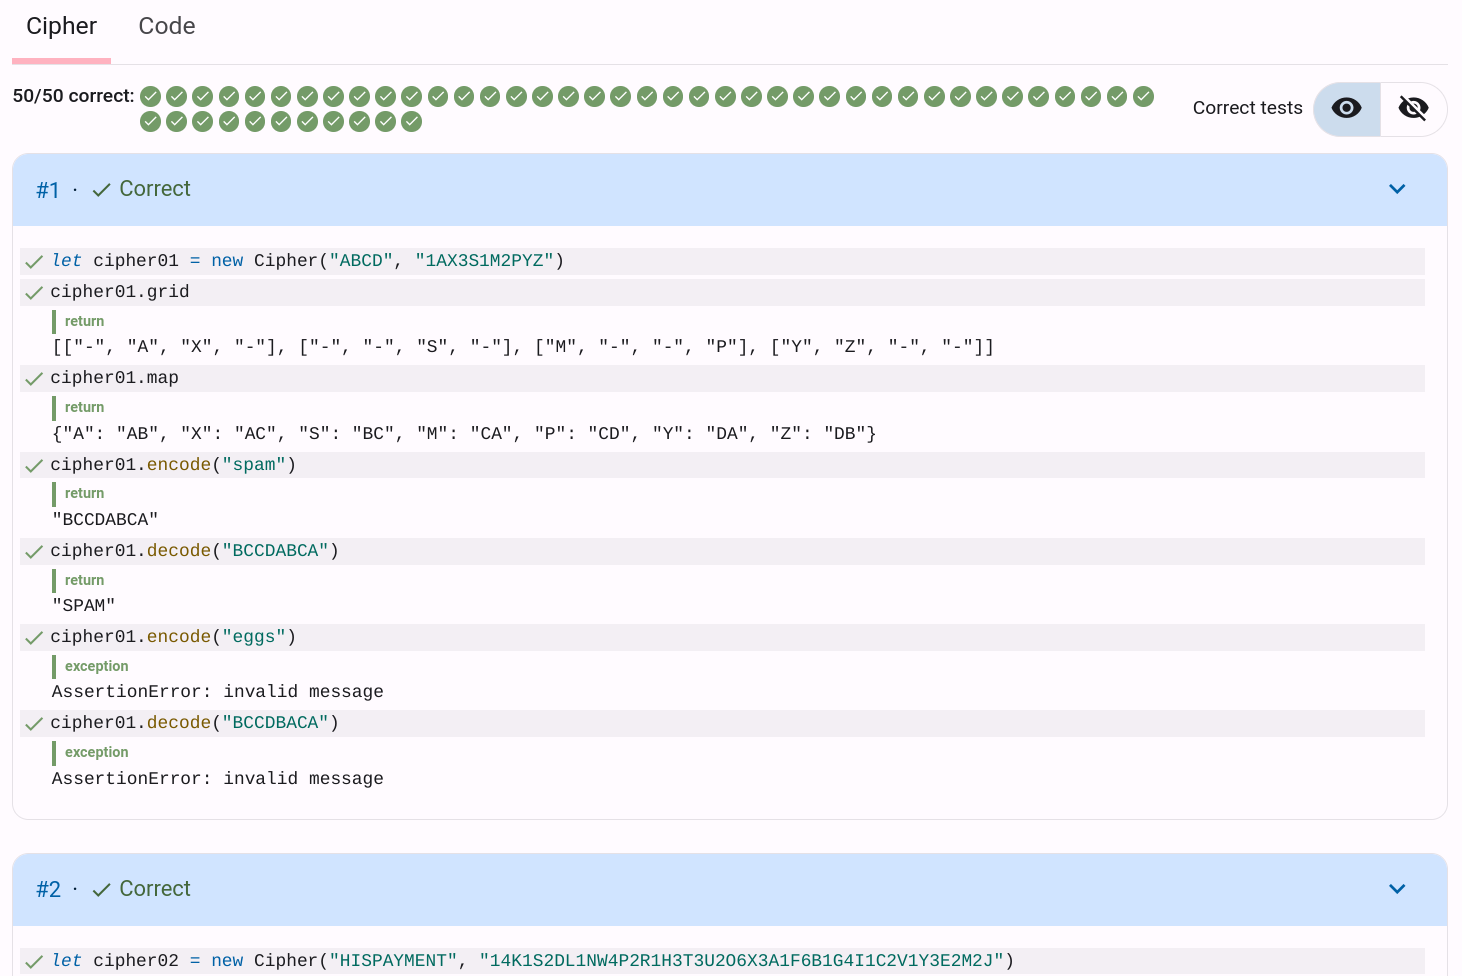
\includegraphics[width=\textwidth]{tested-dsl/render-cipher}
    \caption{
        Dodona rendering of test results after TESTed validated a correct JavaScript submission for the programming exercise configured with the language-agnostic test suite from \cref{lst:cipher-example}.
        All tests from a single test case are visually grouped inside a card.
        Green check marks show that all tests of each script succeeded.
        Each expression has one reported output -- either its return value (\texttt{return}) or a runtime exception (\texttt{exception}) -- that is validated to be correct as indicated by the green colour of the header for the reported output.
    }
    \label{fig:dodona-render-cipher}
\end{figure}

Parallel to dynamic testing, TESTed flags programming errors, bugs, stylistic errors and suspicious constructs by running a language-specific linter (see \cref{subsec:static-analysis-of-the-submission}) on each submission~\autocite{truongLearningProgramWeb2005}.
Dodona displays these linter messages inline in the source code of the submission, in a separate tab called Code.
Linters are preconfigured in the language-specific modules of TESTed, so no additional configuration is needed in the test suite.
Test suites may, however, overrule these linter configurations.

\subsubsection{Recoupling exercise: multiple functions and advanced data types}\label{subsubsec:recoupling-exercise:-multiple-functions-and-advanced-data-types}

\Cref{lst:recouple-example} shows a language-agnostic test suite for an exercise that asks to implement two functions: \texttt{divide} and \texttt{recouple}.\footnote{\url{https://dodona.be/en/activities/1145516160/}}
The first function must divide the given string into a number of parts.
The second function must split each given string and then recombine the corresponding parts into new strings.
As part of the problem-solving process, students may discover a divide-and-conquer strategy: the implementation of the second function may call the first function that solves a subtask.

However, the test suite validates the correct behaviour of both functions in two separate units.
This example illustrates that TESTed-DSL allows leaving out the grouping of tests in a script as a shorthand for the common case of test cases whose script has a single test.
The first two test cases for the \texttt{divide} function (lines 4--7) use the \texttt{return} attribute with flow style notation of a YAML sequence to specify the function call is expected to return a sequence of strings as basic types of TESTed.
As a result, both lists and tuples will, for example, be accepted for Python submissions.
On the contrary, the first two test cases for the \texttt{recouple} function (lines 11--14) use an explicit cast to force the return value to be a list (line 12) or a tuple (line 14) for languages like Python that make the difference.
For Java and JavaScript submissions, however, arrays are accepted in both cases.
The same observation holds for the first argument passed to the function: a list (line 11) or a tuple (line 13) for languages that make the difference, or the default sequence type for other languages.

\begin{listing}
    \begin{minted}{yaml}
units:
  - unit: "Divide"
    scripts:
      - expression: "divide('accost', 3)"
        return: ["ac", "co", "st"]
      - expression: "divide('COMMUNED', 4)"
        return: ["CO", "MM", "UN", "ED"]
      - expression: "divide('programming', 5)"
        exception: "invalid division"
  - unit: "Recouple"
    scripts:
       - expression: "recouple(['ACcoST', 'COmmIT', 'LAunCH', 'DEedED'], 3)"
         return: !list ["ACCOLADE", "communed", "STITCHED"]
       - expression: "recouple(('ACCOLADE', 'communed', 'STITCHED'), 4)"
         return: !tuple ["ACcoST", "COmmIT", "LAunCH", "DEedED"]
       - expression: "recouple(['programming', 'computer', 'games'], 5)"
         exception: "invalid division"
    \end{minted}
    \caption[]{
        Language-agnostic test suite to validate correct behaviour of submissions that must define the functions \texttt{divide} and \texttt{recouple}.
        Because each test case has a single test, grouping of tests in a script can be left out from the test suite specification as a shorthand.
    }
    \label{lst:recouple-example}
\end{listing}

Separating validation of the two functions across two separate units allows students to pinpoint immediately from the feedback what functions already behave as expected.
\Cref{fig:dodona-render-recouple} shows a Dodona rendering of the generated feedback for a Python submission whose implementation of the first function passes all tests.
However, the second function has three tests that fail for different reasons.
The first function call returns the correct result, but also writes the string \texttt{spam} to standard output (\texttt{stdout}) whereas no output is expected on this output stream.
The second function call returns a list where a tuple was expected.
The third function call should throw an exception, but this does not happen.

\begin{figure}
    \centering
    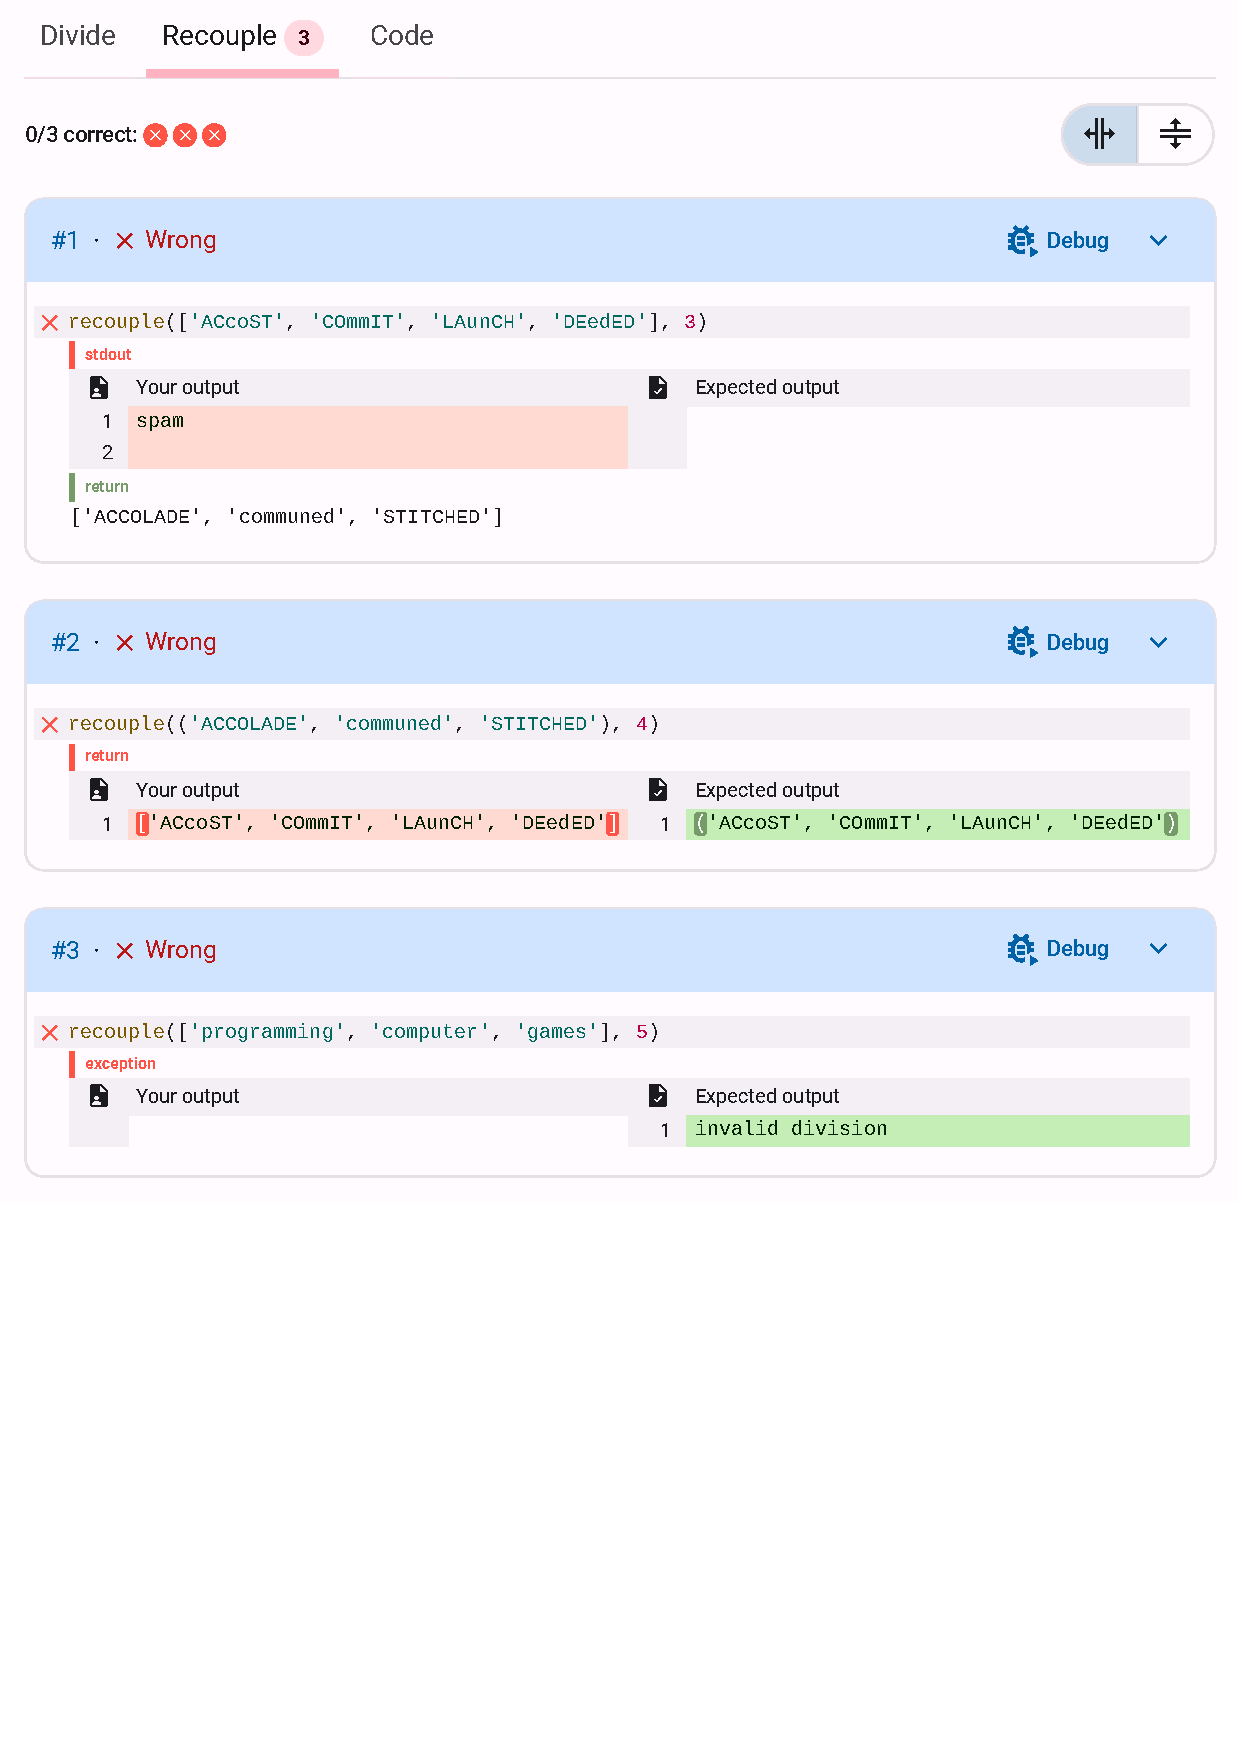
\includegraphics[width=\textwidth]{tested-dsl/render-recouple}
    \caption{
        Dodona rendering of test results after TESTed validated a wrong Python submission for a programming exercise configured with the language-agnostic test suite from \cref{lst:recouple-example}.
        All test cases succeed for the implementation of the function \texttt{divide}, but for different reasons, some test cases fail for the implementation of the function \texttt{recouple}.
        An extra badge in the tab header displays the number of failing test cases in the corresponding unit, or the number of source code annotations in case of the Code tab (none in this case).
    }
    \label{fig:dodona-render-recouple}
\end{figure}

\subsubsection{Sum of three cubes exercise: input/output testing and custom oracles}\label{subsubsec:sum-of-three-cubes-exercise:-i/o-stream-testing-and-custom-oracles}

\Cref{lst:sum-example} shows a test suite for an input/output exercise that asks to read an integer \textit{k} from standard input and write a solution of the sum of three cubes problem ({\addfontfeature{Numbers=Lining}\textit{x}\textsuperscript{3}\,+\,\textit{y}\textsuperscript{3}\,+\,\textit{z}\textsuperscript{3}\,=\,\textit{k}}) to standard output as three lines containing non-zero integers \textit{x}, \textit{y} and \textit{z}~\autocite{bookerCrackingProblem332019}.
The test suite has one unit with three test cases whose script only specifies a single line of input streamed into standard input of the main call and three expected lines of output printed on standard output.
So again the shorthand structure applies here for units and scripts.

The first two test cases show different YAML alternatives for specifying multi-line strings (line 4 and lines 6--9) as the expected value streamed to standard output.
However, specifying a fixed expected output is problematic for this exercise.
The task description does not imply any order in which the three integers must be listed, so any permutation of the three integers given by the expected solution for the second test case should also be validated as a correct solution.
Moreover, some values of \textit{k} have alternative solutions, irrespective of permutations.
For example, another way to solve the first test case is given by {\addfontfeature{Numbers=Lining}(−5)\textsuperscript{3}\,+\,4\textsuperscript{3}\,+\,4\textsuperscript{3}\,=\,3}~\autocite{sutherlandSumsThreeCubes2019}.

As enumerating all possible solutions (and their permutations) is infeasible, the specification of the third test case provides a better approach.
TESTed uses the function \texttt{sum\_of\_three\_cubes} from the Python module \texttt{oracle.py} as a custom oracle to validate the correctness of the output generated on stdout.
TESTed always passes the actual output and some metadata, such as the programming language, and the expected output as the first argument to the oracle.
Additionally, extra arguments taken from the test suite can be passed (in this case there is only one extra argument: the integer \texttt{42}).

\begin{listing}
    \begin{minted}{yaml}
- unit: "Sum of three cubes"
  scripts:
    - stdin: "3"
      stdout: "1\n1\n1\n"
    - stdin: "33"
      stdout: |
        8866128975287528
        -8778405442862239
        -2736111468807040
    - stdin: "42"
      stdout:
        data: |
          -80538738812075974
           80435758145817515
           12602123297335631
         oracle: custom_check
         name: "sum_of_three_cubes"
         file: "oracle.py"
         arguments: [42]
    \end{minted}
    \caption[]{
        Language-agnostic test suite to validate correct behaviour of submissions for an input/output exercise that asks to read an integer \textit{k} from standard input and write a solution of the sum of three cubes problem {\addfontfeature{Numbers=Lining}\textit{x}\textsuperscript{3}\,+\,\textit{y}\textsuperscript{3}\,+\,\textit{z}\textsuperscript{3}\,=\,\textit{k}} to standard output as three lines containing non-zero integers \textit{x}, \textit{y} and \textit{z}.
    }
    \label{lst:sum-example}
\end{listing}

The custom oracle needs to
\begin{enumerate*}[label=\emph{\roman*})]
    \item check the output string has the correct format (three lines containing one integer each),
    \item parse the three integers \textit{x}, \textit{y} and \textit{z} from the output (converting their string representation into integers) and
    \item check the integer expression {\addfontfeature{Numbers=Lining}\textit{x}\textsuperscript{3}\,+\,\textit{y}\textsuperscript{3}\,+\,\textit{z}\textsuperscript{3}} yields the value of the second argument (\texttt{42}).
\end{enumerate*}
Passing an extra argument is not strictly needed here as the custom oracle could also derive the data from the expected value, using the same procedure as used to derive the data from the actual value.

\subsection{Language-agnostic task descriptions}\label{subsec:example-language-agnostic-task-descriptions}

\Cref{lst:task-description-markdown} shows a language-agnostic task description for the \textit{Recoupling} exercise that was introduced in \cref{subsubsec:recoupling-exercise:-multiple-functions-and-advanced-data-types}.
The task description is specified using Kramdown-flavored Markdown.
It contains Jinja2 placeholders (\mintinline{jinja}{{{code}}}) for function names and formal/informal names of data types, along with MathJax placeholders (\mintinline{jinja}{$$...$$}) for \LaTeX{} formulae.
The task description ends with some examples of the expected behaviour when calling the two functions \texttt{divide} and \texttt{recouple} that must be implemented for this programming exercise.
The language-agnostic specification of the sample code is denoted using the same specification of the test suite for the programming exercise in TESTed-DSL format or a reduced version thereof (see \cref{lst:recouple-example}).

\begin{listing}
    \begin{minted}[fontsize=\footnotesize]{jinja}
Write a function `{{function('divide')}}` that takes two arguments: _i_) a word (`{{datatype('text')}}`) and _ii_) the number of (non-overlapping) groups $$n \in \mathbb{N}_0$$ (`{{datatype('integer')}}`) into which the word must be divided. If the word passed to the function `{{function('divide')}}` cannot be divided into $$n$$ groups that have the same length, an exception must be raised with the message `invalid division`. Otherwise, the function must return a {{datatype('list').singular}} (`{{datatype('list')}}`) containing the $$n$$ groups (`{{datatype('text')}}`) into which the given word can be divided. All groups need to have the same length (same number of letters).

Write another function `{{function('recouple')}}` that takes two arguments: _i_) a {{datatype('sequence').singular}} (`{{datatype('sequence')}}`) of $$m \in \mathbb{N}_0$$ words (`{{datatype('text')}}`) and _ii_) the number of (non-overlapping) groups $$n \in \mathbb{N}_0$$ (`{{datatype('integer')}}`) into which the words must be divided. If at least one of the words passed to the function `{{function('recouple')}}` cannot be divided into $$n$$ groups that have the same length, an exception must be raised with the message `invalid division`. Otherwise, the function must return a {{datatype('sequence').singular}} containing the $$n$$ new words (`{{datatype('text')}}`) obtained when each of the $$m$$ given words is divided into $$n$$ groups that have the same length, and if each of the $$m$$ corresponding groups is merged into a new word. The type of the returned {{datatype('sequence').singular}} (`{{datatype('sequence')}}`) must correspond to the type of the {{datatype('sequence').singular}} passed as a first argument to the function.

### Example

```dsl

```
    \end{minted}
    \caption[]{
        Language-agnostic task description for the \textit{Recoupling} exercise.
        The Kramdown-flavored Markdown contains Jinja2 placeholders for function names and both formal and informal names of data types.
        The task description ends with some examples that illustrate how the two functions should be used.
        The sample code is denoted using the same specification of the test suite for the programming exercise in TESTed-DSL format (\cref{lst:recouple-example}).
    }
    \label{lst:task-description-markdown}
\end{listing}

For the sample code in the template, we use the Jinja2 import facilities to include the test suite from \cref{lst:recouple-example}.
TESTed will automatically generate an example based on this test suite, while ignoring structural elements (like the hierarchy).

Starting from a task description template, the TESTed template engine can generate language-specific versions of the task description for all supported programming languages (\cref{fig:dodona-render-task-description}).
This is done by taking into account language-specific conventions (naming, quoting, formal and informal names and syntax for literals, expressions, and statements) as specified in the language modules for the supported programming languages.
This dual use between test suites and task description keeps the language-specific modules of TESTed lightweight and guarantees consistency between the generation of language-specific tests and descriptions.

\begin{figure}
    \begin{wide}
        \begin{tikzpicture}
            \node[anchor=south west,inner sep=0] (image1) at (0,0) {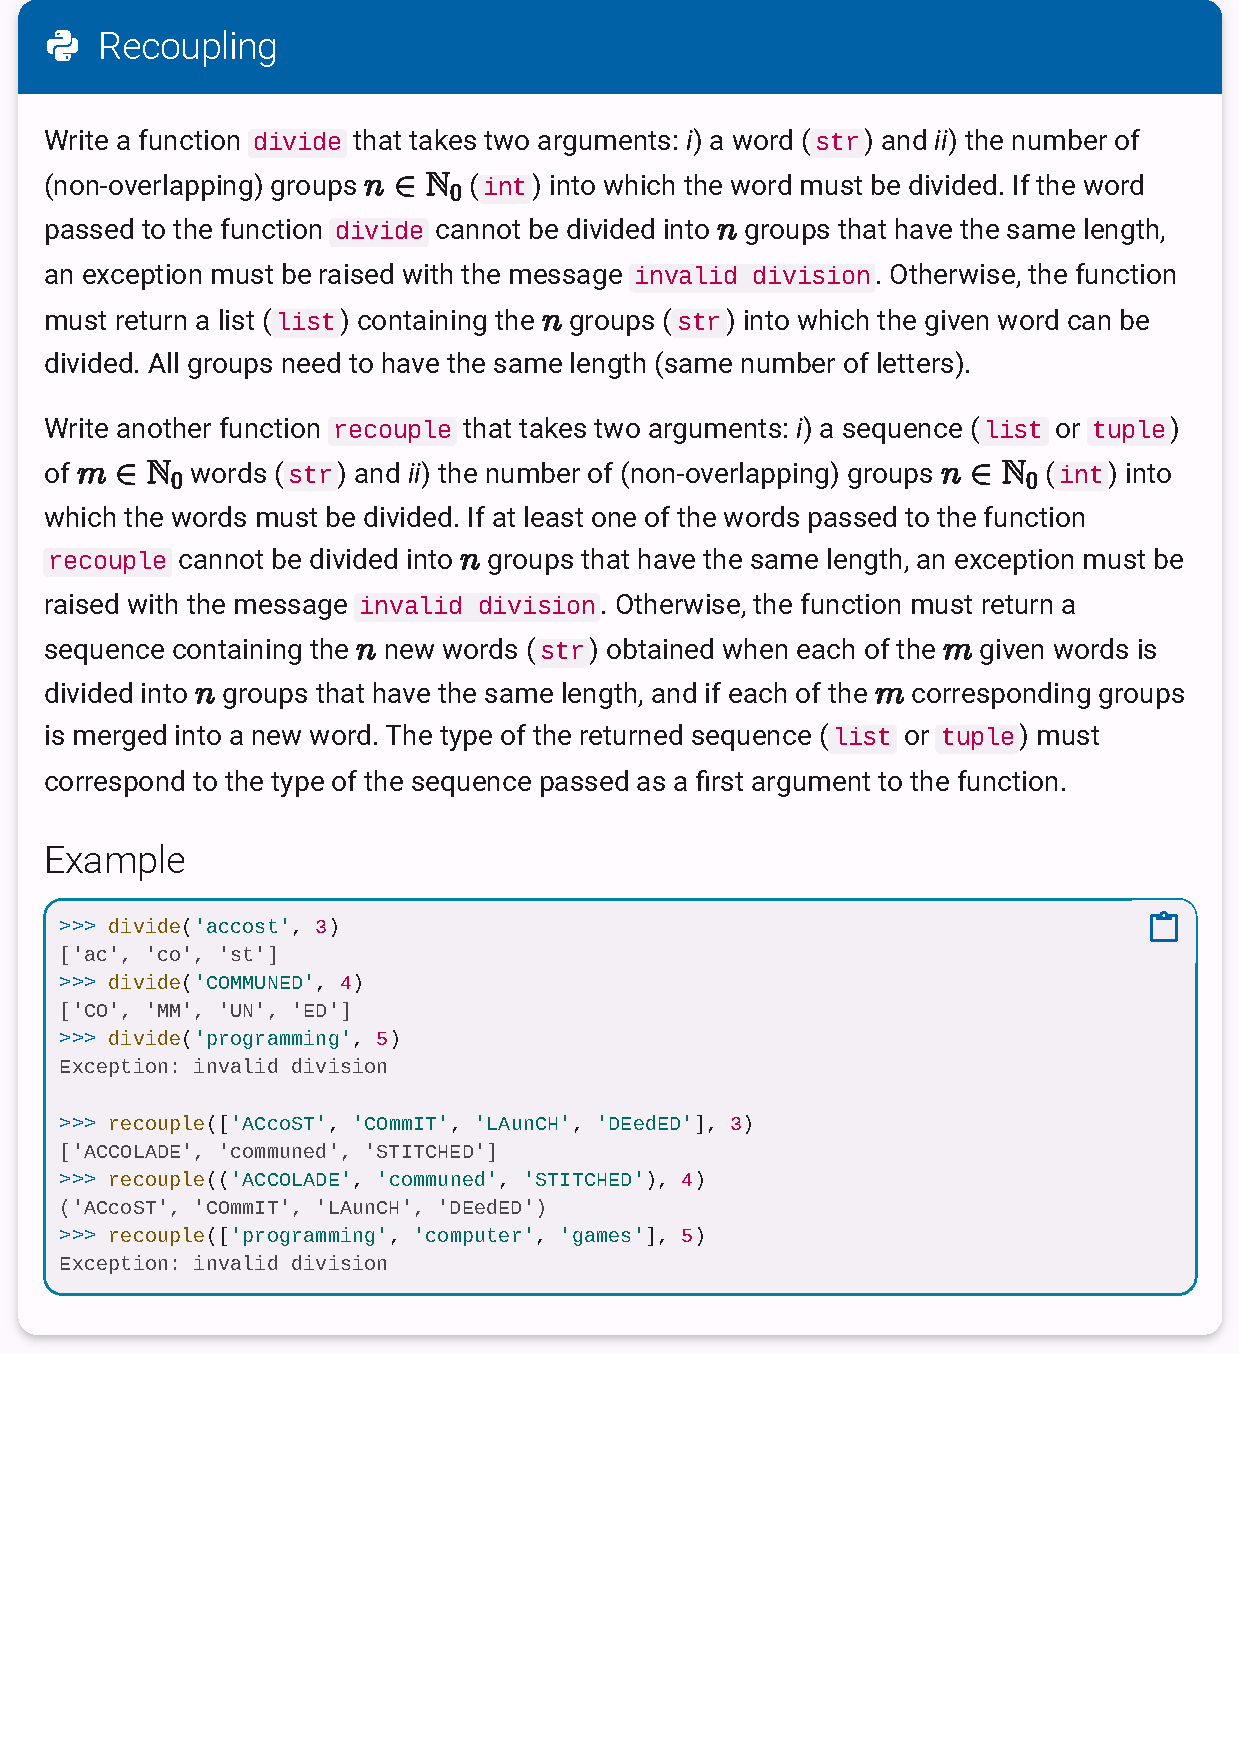
\includegraphics[width=0.65\linewidth]{tested-dsl/recoupling-py}};
            \node[anchor=south west,inner sep=0] (image2) at (0.35\linewidth,-5) {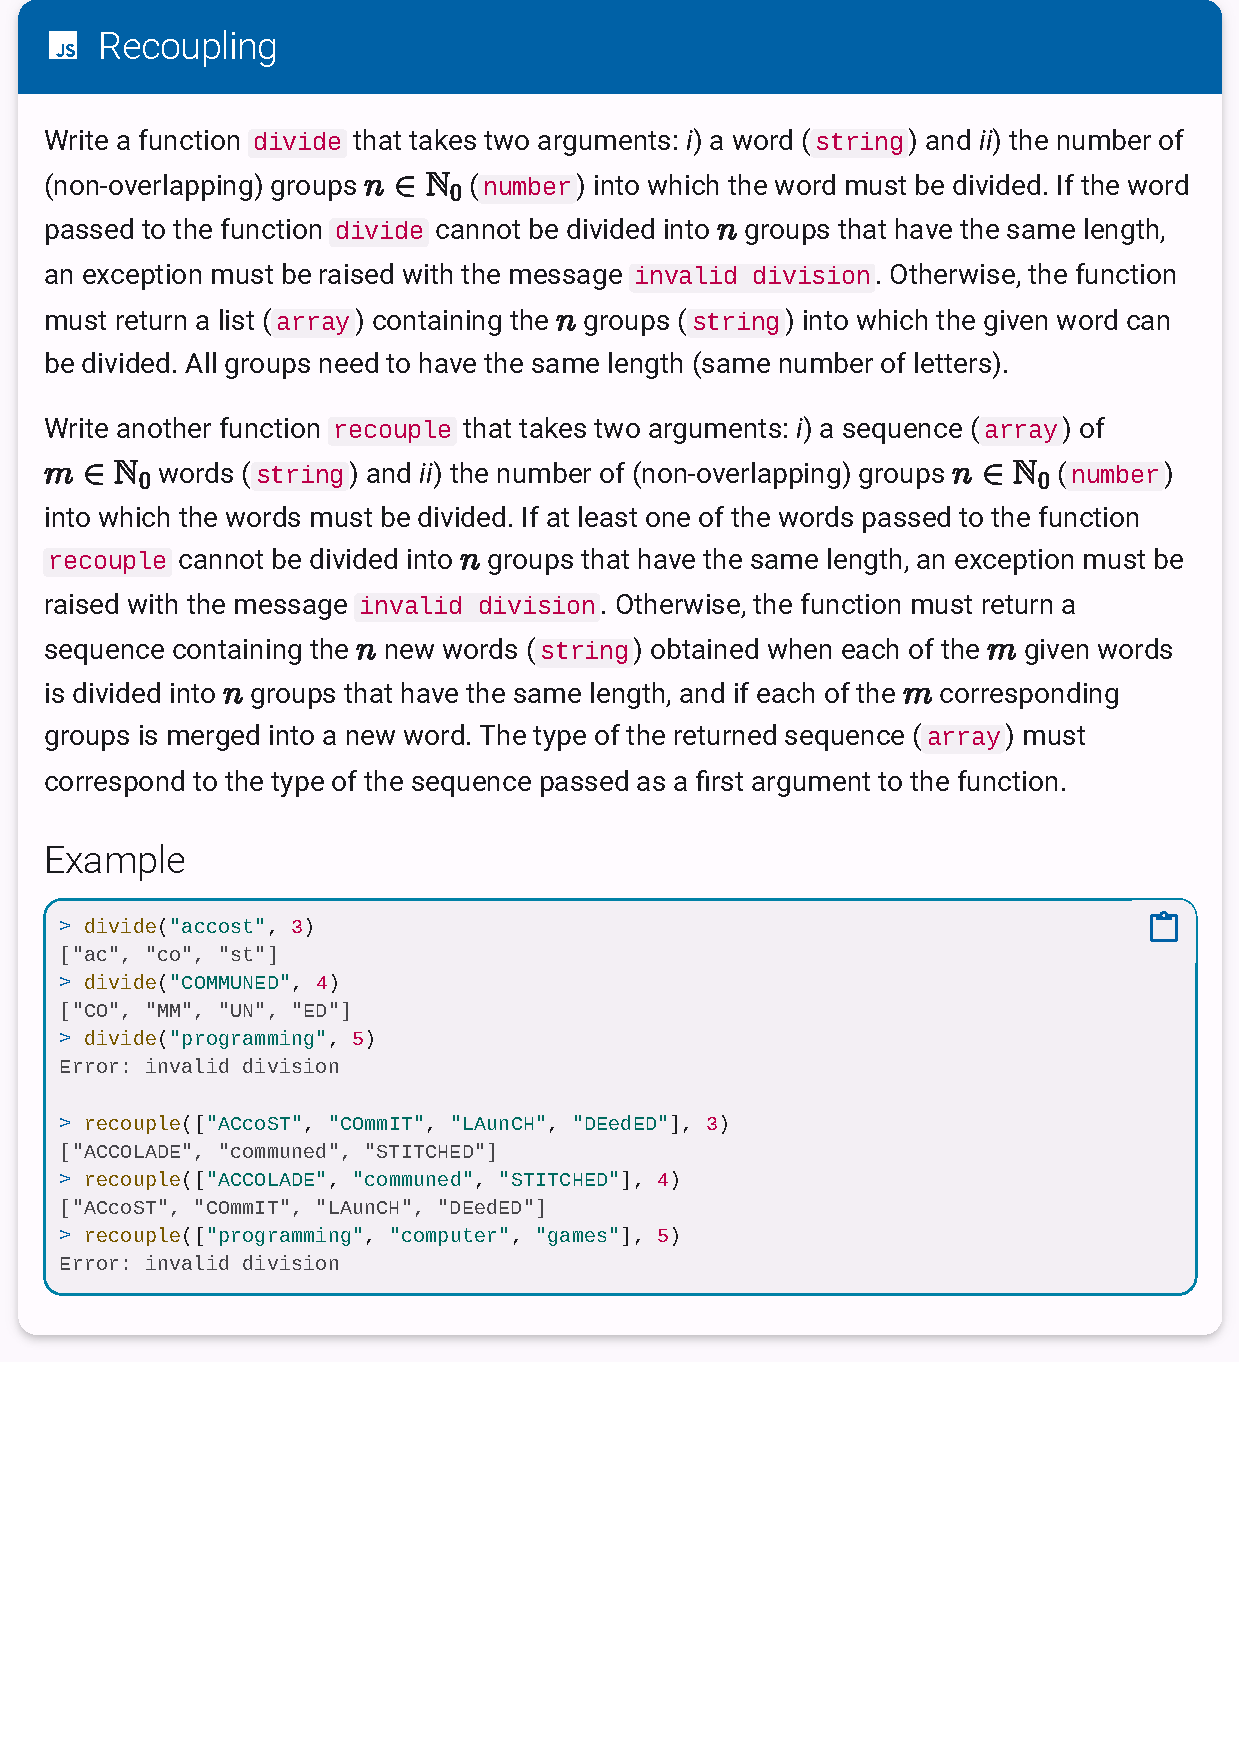
\includegraphics[width=0.65\linewidth]{tested-dsl/recoupling-js}};
        \end{tikzpicture}
    \end{wide}
    \caption{Dodona rendering the Python (top left) and JavaScript (bottom right) versions of the task description as generated by the template engine of TESTed.}
    \label{fig:dodona-render-task-description}
\end{figure}

\section{Evaluation}\label{sec:dsl-evaluation}

During the academic year 2023--2024 we started promoting TESTed with TESTed-DSL as the primary way to author new (language-agnostic) programming exercises on Dodona~\autocite{vanpetegemDodonaLearnCode2023}.
We clearly documented the process, including guides and reference documentation.\footnote{\url{https://docs.dodona.be/nl/guides/exercises/} (some documentation is currently only available in Dutch).}
At the time of writing, \num{1124} programming exercises on Dodona support automated assessment through TESTed, with \num{333195} assessed student submissions (\cref{tab:exercises-on-dodona}).

\begin{table}
    \centering%
    \caption{Dodona programming exercises using TESTed for automated assessment.\label{tab:exercises-on-dodona}}%
    \addfontfeature{Numbers={Lining, Monospaced}}
    \small%
    \begin{tabular}{|l|r|r|}
        \hline
        \textbf{Programming language}   & \textbf{№ of exercises}   & \textbf{№ of submissions} \\
        \hline
        Bash                            & \num{32}                  & \num{121011}              \\
        C                               & \num{83}                  & \num{652}                 \\
        C\#                             & \num{1}                   & \num{6}                   \\
        Haskell                         & \num{86}                  & \num{241}                 \\
        Java                            & \num{120}                 & \num{1493}                \\
        JavaScript                      & \num{271}                 & \num{178011}              \\
        Kotlin                          & \num{146}                 & \num{271}                 \\
        Python                          & \num{385}                 & \num{31510}               \\
        \hline
        \textbf{Total}                  & \textbf{\num{1124}}       & \textbf{\num{333195}}     \\
        \hline
    \end{tabular}
\end{table}

In the next sections, we look into a case study where we converted all JavaScript exercises of a course to use TESTed-DSL\@.
This resulted in \num{72} programming exercises and \num{22018} student submissions (these are part of the total numbers shown in \cref{tab:exercises-on-dodona}).

\subsection{Expressiveness and ergonomics}\label{subsec:dsl-expressiveness-and-ergonomics}

To evaluate the expressiveness of TESTed-DSL and its applicability in educational practice, we authored test suites for a collection of \num{72} programming exercises that were used during the 2023 spring semester in an introductory course at Ghent University taken by \num{114} students.\footnote{\url{https://dodona.be/en/courses/2263/}}
None of these exercises is based on input/output, \num{22} ask to implement one or more functions and \num{50} ask to implement one or more classes.

The largest part of the collection consists of all the \num{66} JavaScript exercises we designed for this course over the years.
These exercises already supported automated assessment with a test suite designed for a custom JavaScript-specific testing framework.
To migrate automated assessment for these exercises to TESTed, we wrote a script that either converts their existing JavaScript test suites into a TESTed-DSL specification or reports why this is not possible.
Seamless automated conversion was helped by the fact that we designed TESTed according to best practices we obtained from designing and implementing many language-specific testing frameworks for Dodona, and a generic feedback format (JSON) that closely follows the structure of TESTed-DSL test suites.

All existing test suites for these JavaScript exercises could be transformed into TESTed-DSL: \num{58} of \num{66} (\qty{88}{\percent}) into language-agnostic test suites and \num{8} of \num{66} (\qty{12}{\percent}) into JavaScript-specific test suites.
The latter use JavaScript-specific language constructs that are not (yet) supported by TESTed: array indexing, object indexing, array destructuring assignment, object identity checking (\mintinline{javascript}{===} operator), class constants, spread syntax (\mintinline{javascript}{...} operator), and the use of arrow functions as callbacks.
The sample solutions for the programming exercises -- assumed to be correct -- were used for testing the test suite migration throughout the process.

Although the above experiment made clear that most, but not all, test suites for existing JavaScript exercises could be converted into language-agnostic test suites for TESTed, TESTed-DSL was expressive enough to also specify JavaScript-specific test suites for the remaining exercises.
At least we may conclude from this experiment that for our practice, we can gradually deprecate language-specific testing frameworks in favour of TESTed.
Along the way, converting test suites into a language-agnostic TESTed-DSL specification also broadens the usability of the programming exercises across programming languages.

We also added 6 new programming exercises with language-agnostic TESTed-DSL test suites to the collection, designed from scratch and used for a midterm test (2 exercises) and for 2 exam sessions (2 exercises each) during the semester.
Our experience in doing so is that direct authoring of TESTed-DSL test suites is ergonomic, either when done by hand or using a generator script based on a correct solution.
Human error is reduced by using the formal specification for automatic verification that TESTed-DSL test suites are well-formed and valid.
TESTed performs such verification while parsing test suites, but this can also be done interactively while authoring the test suites in an \textsc{ide}.
For example, we provide a VS Code Plugin that automatically applies the JSON Schema to the YAML files to catch errors and to provide autocompletion.\footnote{\url{https://marketplace.visualstudio.com/items?itemName=dodona.dodona-exercise-plugin}}
The improved readability of TESTed-DSL test suites further increases productivity and enhances comfort while authoring programming exercises, especially with editor support for syntax highlighting and autocompletion.

Of these exercises, \num{19} were used as mandatory assignments during the 2023 spring semester of the introductory course and \num{6} for midterm tests and exams.
Students could use the remaining exercises from the collection for additional practice in preparation for tests and exams.
Students were not restricted in the number of submissions for each exercise.
They received immediate feedback from automated assessment upon each submission, also after the submission deadline and also during midterm tests and exams.
Students had previous experience in working with Dodona for solving Java, Python and Bash programming exercises with automated assessment.
But most of them had no prior experience with the collection of JavaScript exercises, nor with automated assessment based on the custom JavaScript-specific testing framework used in previous editions of the course.

For each course edition, we make a different selection of mandatory exercises and we always design new exercises for midterm tests and exams.
This way, students who had to retake the course had no reference for comparison between the custom JavaScript-specific testing framework used in previous course editions and TESTed using during the 2023 edition.
For that reason, we decided not to inform students about us switching the JavaScript testing framework that for them runs as a hidden component in the backend of Dodona.

In total, TESTed automatically assessed \num{22018} JavaScript submissions during the 2023 spring semester of the course.
None of the questions we received from students during the hands-on sessions for the course or via Dodona's \textcsc{Q\&A} module hinted at any issues with automated assessment or the feedback it generated other than content-related issues.
We also found no indications of problems in the course evaluation that students complete some weeks after the end-of-semester exams.

\subsection{Performance}\label{subsec:dsl-performance}

As is the case for software testing in general, the user experience of educational software testing depends on the performance of test runs to limit how long students must wait before feedback is reported~\autocite{sarsaSpeedingAutomatedAssessment2022}.
We therefore ran a benchmark using all 72 JavaScript exercises mentioned previously to validate the performance of TESTed.
These exercises have 95 test cases on average, with a minimum of 2 and a maximum of 518.
Previously, we showed that the extra flexibility provided by language-agnostic testing comes with an acceptable overhead when dynamically generating test code for language-specific test harnesses (\cref{subsec:tested-in-educational-practice}).
Here, we specifically investigated if using a domain-specific language for specifying test suites incurs additional overhead compared to using the JSON-formatted test suite specifications introduced in version 1.0 of TESTed.
The latter specifications closely reflect the internal structure and functionality of the testing framework, whereas TESTed-DSL was designed to make test suite authoring as ergonomic as possible.

The benchmark was run on a laptop running Linux (NixOS version 24.05) with \qty{32}{\gibi\byte} \textsc{ram}, an Intel i7-11850H processor, and a \qty{1}{\tebi\byte} \textsc{ssd}.
No power-saving features were active during the benchmark.
It turns out that parsing and processing of TESTed-DSL test suites takes \qty{20}{\percent} less time on average compared to the original \textsc{json}-formatted test suites.
We believe this is mainly due to using a more performant YAML parsing library compared to the Python built-in JSON parsing library.
However, this illustrates TESTed-DSL does not incur any additional overhead compared to the original JSON format.
Because the domain-specific language still supports all features of TESTed, we decided to deprecate support for JSON-formatted test suites in favour of TESTed-DSL\@.

Equally important is the total runtime for assessing the submissions for a programming exercise.
This is the time students must wait before feedback is available.
We observed that \qty{75}{\percent} of all JavaScript exercises are assessed automatically in less than 725 ms (\cref{fig:dsl-performance}).
On average, TESTed spends \qty{225}{\milli\second} parsing and processing a TESTed-DSL test suite, with the remaining time used for generating test code (language-specific test harnesses), running test code and checking test results.
Due to additional speedups in the testing framework itself, TESTed 2.0 is up to 2.8 times faster than TESTed 1.0 (both using JSON test suites).\footnote{\url{https://github.com/dodona-edu/universal-judge/pull/334}}

\begin{figure}
    \centering
    \includestandalone{tested-dsl/performance}
    \caption{
        Histogram and box plot of the total runtime for automatically assessing the (correct) sample solutions with TESTed for all \num{72} JavaScript exercises.
        Half of the programming exercises have their submissions assessed in the range of \SIrange{360}{725}{\milli\second}, with \qty{75}{\percent} of the assessments taking less than \qty{725}{\milli\second}.
    }
    \label{fig:dsl-performance}
\end{figure}

\section{Results and contributions}\label{sec:dsl-results-and-contributions}

In this section, we discuss TESTed-DSL and its impact on authoring test suites and task descriptions for programming exercises that support automated assessment.
Apart from its application in authoring language-agnostic task descriptions, the three main contributions of TESTed-DSL for authoring test suites are in expressing how the requirements of programming exercises must be assessed.
Its test suites:

\begin{enumerate}
    \item share the exact same declarative structure and functionality across programming languages,
    \item bridge between input/output testing (black-box, weakly typed) and unit testing (white-box, strongly typed), and
    \item can express the test code in a language-agnostic way.
\end{enumerate}

The first contribution might be of general interest to the broader software engineering community, but the last two contributions are especially relevant for computer science education.
In the following subsections, we discuss the impact of each contribution.

For task descriptions, many of the same benefits apply as for test suites.
Specifically, the application of the domain-specific language to task descriptions allows for programming language agnostic representations of code references: names of constructs (functions, classes, properties, etc.) and data types (e.g.\ lists, sets).
Additionally, code fragments written in the abstract language can be automatically converted to code fragments of the target programming language.

\subsection{Declarative structure}\label{subsec:dsl-declarative-structure}

Most programming languages have one or more unit testing frameworks, whose structure and functionality are predominantly derived from Smalltalk's SUnit~\autocite{beckSimpleSmalltalkTesting1997}.
Collectively the latter are known as xUnit~\autocite{meszarosXUnitTestPatterns2007}.
xUnit frameworks are code-driven as their test suites express both the structure and the behaviour of tests in the same programming language as the software under test.
Strong coupling to the language of the software under test is natural as behavioural tests must access its public interfaces.

In contrast, TESTed-DSL separates these two concerns by expressing the structure of test suites in a declarative way (in YAML).
TESTed implements the functionality for processing this structural part of test suites in its core module, so only a single highly-optimized implementation is needed for this shared functionality of unit testing across programming languages.
Functionality that remains language-dependent is the generation of test harnesses.
But TESTed splits that across its core module generating language-agnostic harnesses and language-specific modules generating language-specific harnesses, to keep the language-specific modules as lightweight as possible and to share common functionality.

TESTed allows specifying language-specific test suites using TESTed-DSL that share the same structure across programming languages.
TESTed simply has to copy the language-specific attributes when generating language-specific test harnesses.
As an example, \cref{lst:javascript-test-suite} shows a JavaScript-specific version of the test suite from \cref{lst:cipher-example}.
Test suites guiding automated assessment for the same exercise in other programming languages supported by TESTed, only differ in their representation for statements of the test scripts (\texttt{expression}, \texttt{statement}), expected values for strongly typed outputs (\texttt{return}, \texttt{exception}) and strongly typed arguments passed to custom oracles (\texttt{arguments}).
The programming language in which these attributes (blue background) are expressed is specified with the \texttt{language} attribute (line 2) that is inherited across the hierarchy of the test suite.

\begin{listing}
    \begin{minted}[escapeinside=@@]{yaml}
unit: "Cipher"
language: @\hl{"javascript"}@
cases:
  - script:
      - statement: @\hl{"const cipher = new Cipher('ABCD', '1AX3S1M2PYZ')"}@
      - expression: @\hl{"cipher.grid"}@
        return:
         - ["-", "A", "X", "-"]
         - ["-", "-", "S", "-"]
         - ["M", "-", "-", "P"]
         - ["Y", "Z", "-", "-"]
      - expression: @\hl{"cipher.map"}@
        return:
          "Y": "DA"
          "M": "CA"
          "P": "CD"
          "Z": "DB"
          "S": "BC"
          "A": "AB"
          "X": "AC"
      - expression: @\hl{"cipher.encode('spam')"}@
        return: "BCCDABCA"
      - expression: @\hl{"cipher.decode('BCCDABCA')"}@
        return: "SPAM"
      - expression: @\hl{"cipher.encode('eggs')"}@
        exception: "invalid message"
      - expression: @\hl{"cipher.decode('BCCDBACA')"}@
        exception: "invalid message"
  - script:
      # statements and expressions of the second script come here
    \end{minted}
    \caption[]{
        JavaScript-specific test suite to validate correct behaviour of submissions that must define the class \texttt{Cipher}, where the shorthand was applied for test suites having a single unit.
        The JavaScript-specific attributes of this test suite are highlighted in blue.
    }
    \label{lst:javascript-test-suite}
\end{listing}

A single TESTed-DSL test suite can also specify language-specific alternatives for multiple languages, as opposed to using a separate unit testing framework for each language, each with their custom version of the test suite.
\Cref{lst:multiple-test-suite} shows an example with Python and JavaScript alternatives for the same test expression.
This gives access to language-specific features that are not (yet) supported in the abstract programming language of TESTed-DSL or are not (yet) supported by a language-specific module of TESTed.
Here, the former is the case for passing anonymous functions as arguments to functions and converting strings to uppercase.
This example also shows that TESTed-DSL test suites can mix language-specific (lines 2--4) and language-agnostic (line 5) sections.

\begin{listing}
    \begin{minted}[escapeinside=@@]{yaml}
unit: 'Sort words'
expression:                       # language-specific
  python: @\hl[ugent-ps!20!white]{"sort\_words(['SPAM', 'eggs', 'bacon'], lambda word: word.upper())"}@
  javascript: @\hl{'sortWords(["SPAM", "eggs", "bacon"], word => word.toUpperCase())'}@
return: ['bacon', 'eggs', 'SPAM'] # language-agnostic
    \end{minted}
    \caption[]{
        TESTed-DSL test suite to validate correct behaviour of submissions that must either define the function \texttt{sort\_words} in Python or define the function \texttt{sortWords} in JavaScript. The Python-specific sections of this test suite are marked in green and the JavaScript-specific sections in blue.
    }
    \label{lst:multiple-test-suite}
\end{listing}

\subsection{Combined input/output and unit testing}\label{subsec:combined-i/o-stream-and-unit-testing}

The examples in \cref{sec:dsl-illustrative-examples} already show the flexibility of TESTed-DSL to specify test suites for both input/output exercises (\cref{lst:sum-example}) and exercises with fixed internal interfaces (\cref{lst:cipher-example,lst:recouple-example}).
However, individual tests can also combine any mix of weakly and strongly typed input and output channels.
For example, an expression calling a function with arguments, which reads from standard input, accesses main call arguments and environment variables, writes to standard output and error, and returns a value.
In addition, test cases can combine black-box tests for the main call with a test script of white-box tests for statements and expressions that can access internal interfaces of the submission.
This unification of test suites combining strongly/weakly typed and black-box/white-box approaches solves a long-standing problem in educational software testing.

\Textcite{fonteFlexibleDynamicSystem2013} proposed Output Semantic-Similarity Language (OSSL) as a domain-specific language to serialize strongly typed data across weakly typed standard input and output.
Although the formal specification of OSSL resembles the TESTed basic types supported by TESTed-DSL, no OSSL-parser was ever published and it was only conceived for use in language-agnostic input/output testing.
For application in language-specific unit testing, TESTed added the extra layer of advanced types that are also supported by TESTed-DSL\@.
\Textcite{enstromFiveYearsKattis2011} suggest splitting programming exercises with complex tasks over multiple exercises, each testing a separate subtasks via input/output testing.
Compared to the approach taken by TESTed-DSL, this feels like a poor man's version of white-box testing.
It forces students to reveal internal interfaces via standard input and output, and at the same time asks authors to design and maintain alternative instances of an exercise.
An accumulation of extra work, where what we actually seek are ways to reduce the work of authoring and solving programming exercises~\autocite{douceAutomaticTestbasedAssessment2005}.

ACM-ICPC programming contests and derivatives are another area where input/output exercises are regularly used.
These exercises often follow a specific style, with multiple test cases bundled in a single input stream.
This style dates back from times where judges -- as automated software testing frameworks are commonly called in the context of programming contests -- were restricted to a single execution of the submission's main function.
These platforms are heavily used in classrooms~\autocite{wasikSurveyOnlineJudge2018,zinovievaUseOnlineCoding2021}.

Although the ACM-ICPC style of testing can be expressed using TESTed-DSL test suites, it forces students to implement a main function that loops over test cases and bundles their output in a single output stream.
This approach of packing multiple test cases into a single test case further increases the black-box nature of testing.
Additionally, it may propagate faults in the implementation of submissions as a failure for one test case to failures for successive test cases, making it harder to report feedback that easily discerns which individual test cases pass or fail.
In programming contests, limiting feedback to reporting whether all test cases passed is not a concern.

However, in an educational context, we do strive for rich and fine-grained feedback, meaning an automated testing framework designed for contests is less than ideal.
In TESTed-DSL, we essentially move the responsibility for processing multiple test cases from the student to the testing framework.
This is useful for all students, but especially benefits those with limited programming experience.

\subsection{Language-agnostic testing}\label{subsec:language-agnostic-testing}

TESTed-DSL's declarative structure to organize multiple test cases and describe individual test cases already enables authoring programming exercises whose submissions can be automatically assessed across programming languages.
The abstract programming language means that test statements and strongly typed expected outputs can be specified once for all supported programming languages, eliminating repetition for each individual language that is a target for the programming exercise.

The need for language-agnostic software testing is relatively unique to programming exercises, where it is also highly relevant to support automated assessment.
Beyond this educational context, we do not see many use cases for having a single specification to test multiple implementations that differ in programming language.
Those use cases do exist (e.g.\ testing multiple implementations of the same standard), but they are often limited to input/output testing.

Besides online learning platforms supporting computer science courses in secondary and higher education, some platforms target self-learning, programming contests or recruitment~\autocite{hidalgo-cespedesEvaluationOnlineJudge2023}.
Examples include CodeWars\footnote{\url{https://www.codewars.com/}}, Edabit\footnote{\url{https://edabit.com/}}, LeetCode\footnote{\url{https://leetcode.com/}}, CheckIO\footnote{\url{https://checkio.org/}}, Exercism\footnote{\url{https://exercism.org/}} and CodingBat\footnote{\url{https://codingbat.com/}}.
As far as we know, TESTed is the only existing framework that bridges unit testing with language-agnostic testing.
Most other frameworks are either restricted to input/output testing or rely on general-purpose unit testing frameworks.
The input/output-based approach forces students to implement an input/output model in the main function and test oracles to process weakly typed data, and can only evaluate the behaviour of submissions as a whole.

Because general-purpose unit testing frameworks work with language-specific test suites, the alternative approach duplicates efforts in specifying the expected behaviour for a programming exercise to each target programming language of its submissions.
This can be seen in how separate test suites are written for each target language in most programming platforms.

Only Exercism has a mechanism by which some exercises have a single specification in a generic track that is used to automatically derive language-specific instances.\footnote{\url{https://github.com/exercism/problem-specifications}}
This system shares its goals with TESTed-DSL\@.
However, it is far less flexible and ergonomic for authoring programming exercises, as the generation step is needed each time.

\section{Conclusions and future work}\label{sec:dsl-conclusion-and-future-work}

Version 2.0 of TESTed introduces TESTed-DSL as a domain-specific language for writing the test suites that underlie automated assessment, and for writing language-agnostic task descriptions.
We have paid special attention to performance to ensure that TESTed-DSL has no additional overhead compared to JSON test suites (in fact, TESTed-DSL is 1.2 times faster than JSON test suites).
TESTed-DSL itself, apart from its use in authoring language-agnostic task descriptions, has three main contributions: \begin{enumerate*}[label=\emph{\roman*})] \item sharing the same declarative structure across programming languages, \item bridging the gap between input/output testing and unit testing, and \item allowing test code to be expressed in a language-agnostic way.\end{enumerate*}
The first contribution may be of general interest to the broader software engineering community, but the last two contributions are particularly relevant to computer science education.

Our goal is to further develop TESTed as an educational software testing framework for authoring different types of programming exercises across programming languages.
This chapter has focused mainly on dynamic testing, but TESTed also performs compilation and linting as generic types of static testing that are preconfigured in the language-specific modules.
One area of future interest is the introduction of a language-agnostic interface for static code analysis.

We are currently investigating possible extensions to the abstract language of TESTed-DSL, such as operators for testing operator overloading, string conversion, comments, indexing sequences, indexing mappings, destructuring, object identity checking, and object equivalence checking.
There is no need to conservatively restrict the abstract language to features supported by all or most programming languages, as TESTed automatically detects and reports features not supported by a specific programming language or not (yet) implemented by its language module.
Support for additional test inputs (file descriptors, environment variables) and outputs (file descriptors, global scope) is in progress.
We are also investigating native support for pretty printing of nested data structures to make it easier to detect differences between expected and actual return values, and data-driven tests (parameterized tests) to further improve the readability of test suites, support dynamic generation of test data and boost performance of running tests.
Our future roadmap also includes internationalization of named submission interfaces, different ways to measure code coverage, and support for hidden units/test cases that are visible to teachers but remain invisible to students to avoid gaming -- also known as programming to the test~\autocite{pevelerComparingJailedSandboxes2019}.

Further enhancements and improvements of TESTed will be driven by educational practice, with the creation of new programming exercises and the conversion of existing exercises to TESTed-DSL being a major driver.
Feel free to run TESTed as a standalone command line tool, integrate it into your online learning environments, and let us know about interesting use cases.
We ourselves now routinely rely on TESTed to create new programming exercises and to gradually migrate existing exercises to port them to other programming languages and to benefit from the additional features that TESTed brings.
We also switched to TESTed when training (secondary school) teachers how to create programming exercises with automated assessment for Dodona.
First of all because it covers most common cases, is easy to use, and teachers can use the same framework for educational software testing, regardless of their target programming language(s).
As an open-source project on GitHub, we welcome the sharing of unsupported exercise scenarios, bugs and feature requests documented as issues.\footnote{\url{https://github.com/dodona-edu/universal-judge}}
We also welcome additional language-specific modules to support new programming languages.\footnote{\url{https://docs.dodona.be/en/references/tested/new-programming-language/}}

\part{Scratch}\label{part:scratch}

\chapter{The Scratch programming environment}\label{ch:scratch-the-programming-environment}

\dictum[Papert, \textit{Mindstorms}]{In teaching the computer how to think, children embark on an exploration about how they themselves think.}

This chapter is a short introduction to Scratch, both the programming language and the environment.
It also explains how the source code for Scratch is organized.
The main goal is to familiarize the reader with the Scratch environment.
Technical details are given in later chapters where relevant.

\section{The Scratch environment}\label{sec:scratch-environment}

Scratch is a visual programming language and environment~\autocite{resnickScratchProgrammingAll2009}.\footnote{\url{https://scratch.mit.edu}}
Visual programming languages let programmers construct programs by graphically manipulating program elements, rather than textually~\autocite{kelleherLoweringBarriersProgramming2005}.
A subset of visual programming languages are block-based languages, in which programs consist of blocks that are clicked together, not unlike puzzle pieces or Lego bricks~\autocite{weintropBlockNotBlock2015}.
Scratch falls in the category: it consists of a set of blocks with different shapes and colours.
Development on it began in 2002, by the Lifelong Kindergarten research group at the MIT Media Lab.
Scratch became publicly available in 2007 and has been developed by the Scratch Foundation since 2009.
Its target audience is young learners, ages 8 to 16, although it is most commonly used for ages 10 to 14.
It is a widely used programming language: the 2022 annual report of the Scratch Foundation~\autocite{scratchfoundationGrowingGlobalCreative2022} states that there are over 50 million users in the online Scratch community, with 120 million new projects created in 2022.
The official statistics show that in May 2024, there were about 1.5 million active monthly users, with about 3.6 million new projects.\footnote{\url{https://scratch.mit.edu/statistics/}}
In April 2024, the Scratch team announced that the billionth project has been created.\footnote{\url{https://twitter.com/scratch/status/1778814544682295394}}
\makenote*{The TIOBE index is disputed: it is based on the number of reported results in search engines~\autocite{bunceTIOBENotTIOBE2008,sundarramPleaseStopCiting2022,bunceTIOBEIndexBeing2009}.}
The TIOBE index for May 2024 ranks it as the seventeenth most used programming language \autocite{tiobeTIOBEIndexMay2024}.

\begin{figure}
    \begin{wide}
        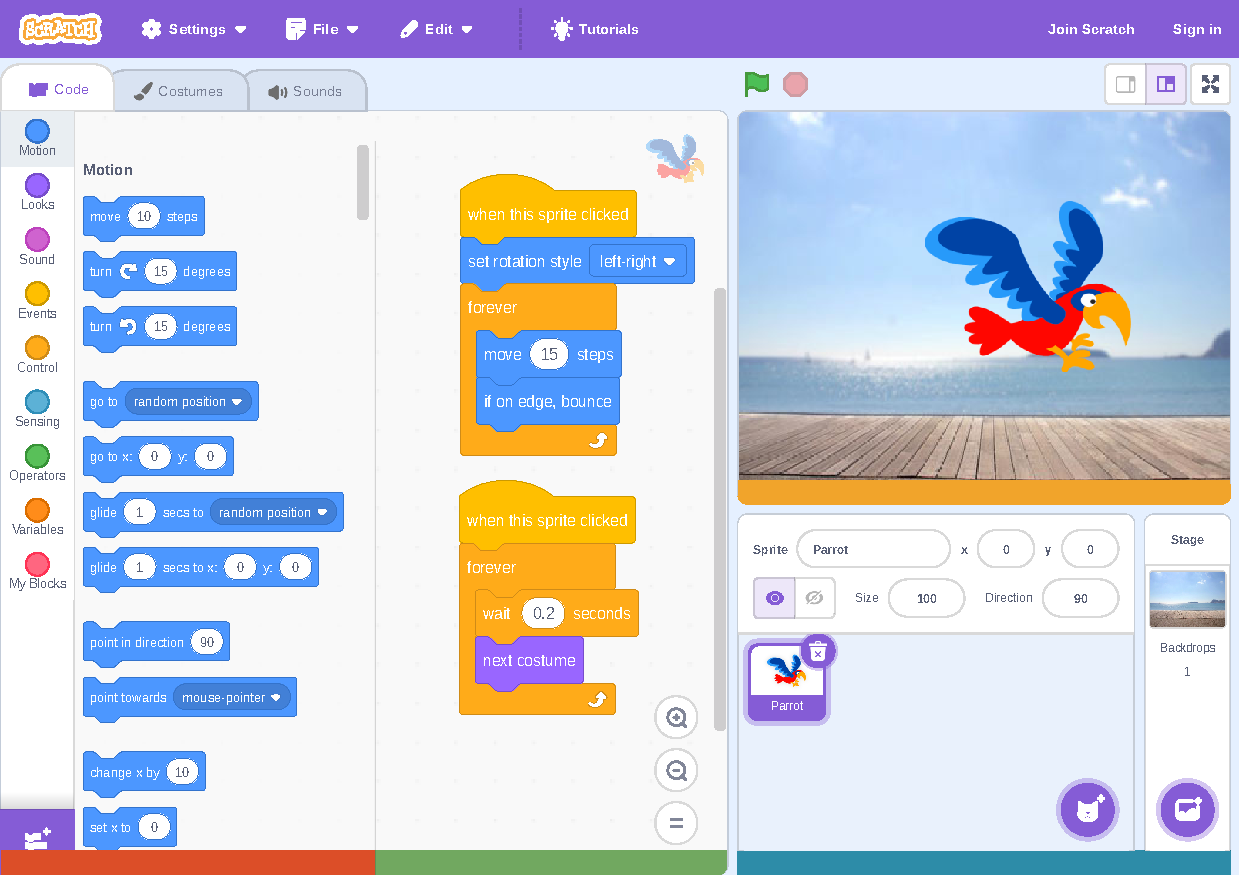
\includegraphics[width=\linewidth]{scratch-introduction/scratch-ide}
    \end{wide}
    \caption{The Scratch environment running an example project.
    The toolbox with the available blocks is underlined in \textcolor{ugent-re}{red}, the workspace is underlined in \textcolor{ugent-ps}{green}, the editors for the sprites and the stage are underlined in \textcolor{ugent-we}{blue}, and the canvas is underlined in \textcolor{ugent-lw}{orange}.}
    \label{fig:scratch-environment}
\end{figure}

\subsection{Using the environment and the blocks}\label{subsec:using-the-environment-and-the-blocks}

Blocks can be dragged from the toolbox on the left side of the integrated development environment (\cref{fig:scratch-environment}) to the workspace in the middle and can be stacked together to form scripts.
Blocks are categorized by their subject or goal: \textcolor{scrmove}{Motion}, \textcolor{scrlook}{Looks}, \textcolor{scrsound}{Sound}, \textcolor{screvent}{Events}, \textcolor{scrcontrol}{Control}, \textcolor{scrsensing}{Sensing}, \textcolor{scroperator}{Operators}, \textcolor{scrvariable}{Variables}, and \textcolor{scrmoreblocks}{My Blocks} (not counting extensions).
Each category has its own colour, except for the blocks that handle lists, as these appear in the \textcolor{scrvariable}{Variables} category but have a different colour.

Each script starts with a hat block that defines when the script should execute.
Scripts can be started as a result of a user action or when a certain criterion is met during the execution of a program, for example, when a clone is started or a message is broadcast.
A common way to start scripts is to press the green flag (\scaledflag{0.8}), which has two functions: it will first stop all running threads before starting new threads for all relevant hat blocks.
The red stop button next to the green flag also stops all currently running scripts.
The green flag button has another functionality: when there are active scripts, the button gets a darker background colour, even if those scripts were not started by the green flag.

Blocks (or parts of scripts) can also be run independently by clicking them.
This illustrates that Scratch is always live: once a project has been loaded, the virtual machine is always running.
Sprites can be moved or manipulated by the user at any time, even if scripts are running.

Each script is connected to a sprite.
Sprites are objects that are drawn on the screen.
The bottom right corner of the environment contains an editor for sprites and the background, which is a special sprite called Stage that is present in every Scratch project.
All scripts corresponding to the selected sprite are shown in the workspace (middle).
The canvas in the top right corner of the environment shows the execution of the project.

Besides the tab for the blocks (the ``code''), there are also tabs for the costumes and sounds.
The costumes are the visual representation of the sprite.
While some blocks control which costume is used, the list of possible costumes must be prepared in this tab in advance.
The sound tab is similar, but for sounds instead of costumes.

Finally, users can manage the sprites and stage at the bottom right.
Sprites can be added and removed (even all sprites) by the user.
Similarly, the ``backdrop'' of the stage (which acts as the costume for the stage) can be modified as well.
Note that the stage cannot be removed.

\subsection{Data types}\label{subsec:scratch-data-types}

Scratch has support for three basic data types: strings, booleans, and numbers~\autocite{maloneyScratchProgrammingLanguage2010}.
A different block shape is used for booleans (a mix between rectangle and diamond) and strings/numbers (round oval).
Variables and reporter blocks (which are special blocks that result in some value) can only be inserted boolean slots if the shapes match.
The string/number slots are less strict: if necessary, Scratch will coerce the data into the right type.
Since the reporter blocks can also use operators, they fulfil the role of expressions.

In addition, Scratch also supports lists with their own set of blocks to manipulate them.
Lists can only contain strings or numbers; booleans are cast to strings.

\subsection{Sprites, the object model}\label{subsec:sprites-the-object-model}

Sprites are the Scratch equivalent to objects~\autocite{maloneyScratchProgrammingLanguage2010}.
As all scripts belong to a particular sprite, almost all blocks only work for the current sprite.
Apparently, an earlier version of Scratch had cross-sprite commands, but users found it confusing.
Since Scratch lacks classes and inheritance, \citeauthor{maloneyScratchProgrammingLanguage2010} call it an ``object-based language''.

The strict separation of code between sprites means there is a lot of work needed to make a set of sprites behave the same way.
For example, a firework might need hundreds of sprites to represent the particles.
Creating copies of the sprites by hand quickly becomes tedious.
That is why Scratch has a clone feature: a ``shadow'' sprite is created that shares its code with the original sprite.
While the code is shared, the execution is not: each clone can execute code independently.
A clone is not visible in the sprite overview, only on the canvas.

Variables are normally also limited to the sprite that defined them and are not visible to other sprites.
There is an exception: the variables of the stage are visible to all sprites and could thus be used for inter-sprite communication.

\subsection{Inter-sprite communication}\label{subsec:intersprite-communications}

\textcolor{screvent}{Broadcasts} are the intended way to let sprites communicate with each other.
There are other ways, such as variables (since variables in the stage are global).
However, broadcasts remain the intended way to do inter-sprite communication.
It is a one-to-many broadcasting system~\autocite{maloneyScratchProgrammingLanguage2010}: a broadcast (an arbitrary string) is sent globally and might trigger multiple scripts (even in different sprites).

\subsection{Defining custom blocks with procedures}\label{subsec:defining-custom-blocks-with-procedures}

Scratch allows defining custom blocks, sometimes called procedures.
This allows the user to define blocks that consist of other blocks, similar to procedures in other languages.
Procedures in Scratch can have parameters that can take arguments, which are available as variables to the blocks of the procedure.
Since the custom blocks are procedures and not functions, they do not have return values.

\subsection{Concurrency and parallelism}\label{subsec:parallelism}

Scratch is a highly concurrent language: every script is akin to a thread and can run concurrently to other scripts, even within the same sprite.
The chosen concurrency model of Scratch has a few advantages but also disadvantages, which we discuss in \cref{subsec:execution-of-a-scratch-program}.

Due to JavaScript's single-threaded nature (the language in which Scratch is implemented), the actual execution of a Scratch program will not be in parallel.

\section{Organization of the source code}\label{sec:scratch-internal}

\begin{figure}
    \begin{wide}
        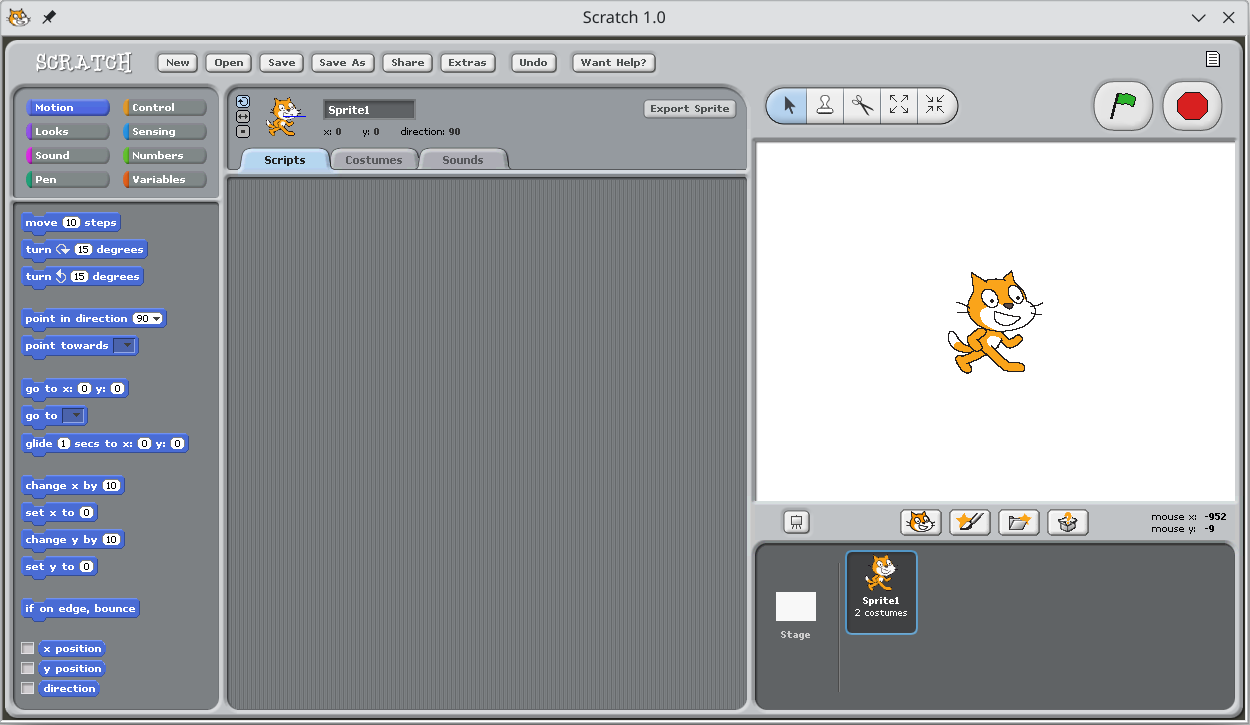
\includegraphics[width=\linewidth]{scratch-introduction/scratch-1}

        \vspace{0.5em}
        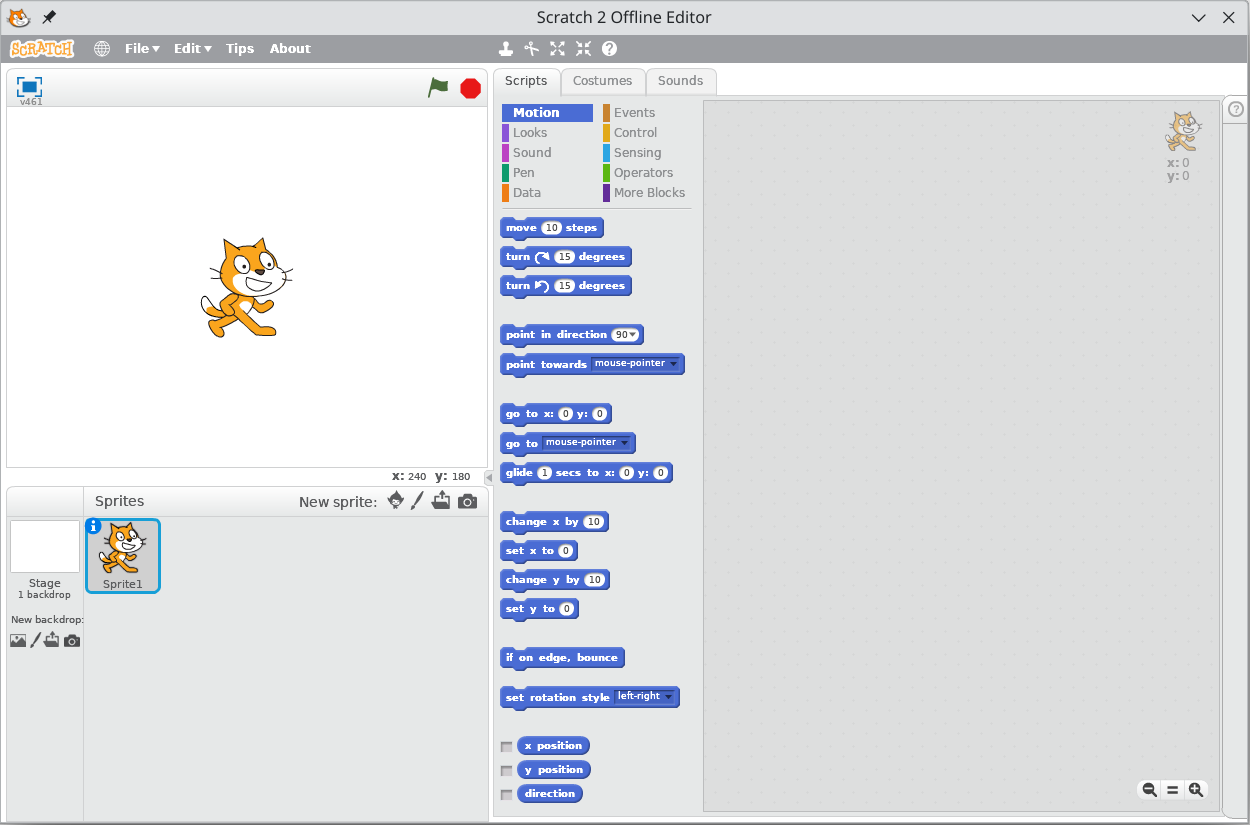
\includegraphics[width=\linewidth]{scratch-introduction/scratch-2}
    \end{wide}
    \caption{The Scratch 1.0 desktop application (top) and Scratch 2.0 offline editor (bottom).}
    \label{fig:scratch-1.0}
\end{figure}


The first public release of Scratch was in May 2007 as a desktop application (\cref{fig:scratch-1.0}), written in Squeak, a Smalltalk implementation.
This version already supported sharing projects by uploading them to the Scratch website.
Scratch 2.0, released in May 2013, was a rewrite providing the first ``online'' version of Scratch (running in the browser).
It used Adobe Flash for the online version and Adobe Air for the downloadable offline editor.

\marginnote{At the time, some users speculated that Scratch 3 was ``rushed'' since it was announced in 2017 that support for Flash would end in 2021. Work on Scratch 3, however, started in May 2016.}
In January 2019, Scratch 3.0 was released.
This version is a complete rewrite, using web technologies, such as JavaScript, HTML, and CSS\@.
Scratch 3.0 is fully browser-based but still supports an offline editor using Electron.\footnote{\url{https://scratch.mit.edu/download}}
Scratch 3.0 consists of a set of independent source code modules that work together to form the complete Scratch environment.
An overview of the relationships between the modules is shown in \cref{fig:scratch-dependencies}.
Each module is developed independently in a separate repository on GitHub.

% Ugly but what can you do
    {
    %! suppress = Makeatletter
    \makeatletter
    \@beginparpenalty=10000
    %! suppress = Makeatletter
    \makeatother
    The most important and relevant modules for this dissertation are:

    \begin{description}
        \item[Scratch Blocks] A fork of Google's Blockly~\autocite{pasternakTipsCreatingBlock2017}, a library for building block-based computing interfaces.\footnote{\url{https://github.com/scratchfoundation/scratch-blocks}}
        \item[Scratch Virtual Machine] The runtime engine behind Scratch and responsible for running the projects created by the blocks.\footnote{\url{https://github.com/scratchfoundation/scratch-vm}}
        \item[Scratch User Interface] A React-based web application that consists of the Scratch programming environment.
        It uses and builds on the other components.\footnote{\url{https://github.com/scratchfoundation/scratch-gui}}
        \item[Scratch Renderer] A WebGL-based renderer, responsible for rendering the canvas.\footnote{\url{https://github.com/scratchfoundation/scratch-render}}
    \end{description}
}

\begin{figure}
    \begin{wide}
        \includestandalone[width=\linewidth]{scratch-introduction/dependencies}
    \end{wide}
    \caption{
        Overview of the dependencies between the Scratch repositories (using their repository name).
        The repositories that are purely for the hosted instance, such as the website, account system, and forum are left out.
        An arrow indicates a dependency.
        For example, the \texttt{scratch-gui} package has five dependencies.
    }
    \label{fig:scratch-dependencies}
\end{figure}

\chapter{A testing framework for Scratch}\label{ch:itch}

\dictum[Flon, \textit{On research in structured programming}]{There does not now, nor will there ever, exist a programming language in which it is the least bit hard to write bad programs.}

Block-based languages like Scratch are popular tools for introducing computer science concepts to young learners~\autocite{bauLearnableProgrammingBlocks2017,zhangSystematicReviewLearning2019}.
The intuitive interface and focus on visuals make Scratch an engaging and accessible programming environment.
Due to this visual nature, syntactical programming errors are eliminated and students can quickly create games, stories, or other projects.
This approach gives students a lot of flexibility to express their creativity.
However, functional errors will still occur~\autocite{zellerWhyProgramsFail2009}.
The process of teaching to code is often slowed down by the delay in providing feedback on and solutions to these errors.

When done manually, assessment of submissions for Scratch exercises is time-consuming and impractical, especially in large classes, where educators often lack the time to give individual feedback to each student.
That is why it is important to equip students with tools that can provide immediate feedback and thus enhance their independent learning skills.
In this chapter, we introduce Itch, a testing framework for Scratch that can act as an automated assessment tool~\autocite{douceAutomaticTestbasedAssessment2005}.

Itch provides flexible testing capabilities: it supports both static and dynamic testing of Scratch projects.
It also provides facilities to make common scenarios easy to test, allowing the educators to focus on testing the interesting parts of an exercise.
We also reflect on Itch's use in an educational context and discuss what testing of Scratch exercises should look like.
On the one hand, Scratch strives to allow maximal creative expression for students, while on the other hand, testable exercises need a well-defined goal and reasonable limits.

\section{Related work}\label{sec:related-work}

In this section, we look at the few existing testing frameworks for Scratch.
Since they are few and far between, we also consider other tools with similar aims: helping students with Scratch.
We begin by looking at the linter-like tools that perform static analysis.

One of the first ones is Hairball~\autocite{boeHairballLintinspiredStatic2013}.
Hairball analyses the blocks of a provided Scratch project, with multiple rules and analysers available.
Dr.\ Scratch~\autocite{moreno-leonDrScratchWeb2015} allows analysing a Scratch project to provide various insights.
For example, Dr.\ Scratch uses Hairball to assign a ``computational thinking score'' to the project, although the creators of Scratch are not a fan of this approach~\autocite{resnickCodingCrossroads2020}, see \cref{subsec:how-to-evaluate-scratch-submissions}.
A similar tool is Ninja Code Village~\autocite{otaNinjaCodeVillage2016}.

QualityHound~\autocite{techapalokulQualityHoundOnline2017} is a linter that detects code smells like ``duplicate code'' or ``broad variable scope''.
In total, twelve code smells are detected.
LitterBox~\autocite{fraserLitterBoxLinterScratch2021} is a newer linter that shares some goals with QualityHound.
For example, it will also detect code smells.
LitterBox supports significantly more patterns and also finds potential bugs~\autocite{fradrichCommonBugsScratch2020}, by looking for code that seems suspicious (for example, comparing two literal values).
Subsequent research has expanded LitterBox to find ``code perfumes''~\autocite{obermullerCodePerfumesReporting2021}, which provides positive feedback to students, for example, by noting good use of loops.

LitterBox can also translate code to LeILa, an intermediate language of the Bastet framework~\autocite{stahlbauerVerifiedScratchProgram2020}.
Bastet uses this intermediate language to enable more traditional and advanced analysis and verification of Scratch programs.
Examples of what the authors envision are automated test generation, data-flow analysis, unbounded model checking on predicate abstraction, and concolic testing.

\marginnote{Unfortunaly, we were not aware of \textsc{itch} when deciding to name our testing framework Itch.}
\textsc{itch}~\autocite{johnsonITCHIndividualTesting2016} is the first automatic testing framework to the knowledge of the authors.
It translates a limited subset of Scratch programs to Python.
\textsc{itch} uses the Scratch say and ask functionality to perform input/output-based testing on Scratch projects.
Of course, being limited to input/output, only a subset of the functionality of Scratch can be used.

Whisker~\autocite{stahlbauerTestingScratchPrograms2019} is a fully automated testing framework for Scratch, and the most similar to Itch.
While manually written test suites (also in JavaScript) are possible, Whisker focuses on automated testing~\autocite{deinerAutomatedTestGeneration2023}.
For example, Whisker (and subsequent research) supports property-based testing, search-based testing~\autocite{deinerSearchBasedTestingScratch2020}, and model-based testing~\autocite{gotzModelbasedTestingScratch2022}.

Finally, Scratch Testing Block~\autocite{nurueTestingExtensionScratch2024} is a prototype for a Scratch extension that provides an ``assert'' block.
It is in aim similar to Poke (\cref{sec:poke:-a-testing-framework-written-in-scratch}): providing testing facilities inside Scratch itself.

Besides Scratch, there are other block-based languages, for some of which testing frameworks also exist.
Block-based languages, like MakeCode~\autocite{ballMicrosoftMakeCodeEmbedded2019}, that compile to another programming language (like Python or JavaScript) are less relevant here, as the testing frameworks often use the compiled version.

Snap\textit{!} is another block-based language~\autocite{monigSnapBuildYour2024}, created in 2011 by a former member of the Scratch team.
It has many features that are considered too advanced for Scratch, like higher order functions, prototype-based programming, nested sprites, and metaprogramming capabilities.
SnapCheck is one testing framework for Snap\textit{!}, inspired by Whisker~\autocite{wangSnapCheckAutomatedTesting2021}.
Another example is CodeMaster~\autocite{wangenheimCodeMasterAutomaticAssessment2018}, which also supports AppInventor (a way to create mobile apps using a block-based language).
However, the actual testing is more similar to Dr.\ Scratch: it assigns scores based on a static analysis of the used blocks.

\section{Introduction to Itch}\label{sec:introduction-to-itch}

Itch is an educational testing framework for Scratch exercises.
Educators can write test suites (in JavaScript) that evaluate a submission to determine if the submission correctly implements the requirements in the problem statement of the exercise.
A submission is the code (in this case the Scratch project) that students submit as the answer to a programming exercise.

Broadly, Itch provides two approaches to testing: static and dynamic tests.
For the static tests, the project is not run: only the blocks are analysed.
With static tests, the test suite can verify (discussed in \cref{subsec:before-execution}):

\begin{itemize}[noitemsep]
    \item If the students did not change some off-limit sprites.
    \item The metadata of the sprites, which sprites exist, their position, their size, their costume, etc.
    \item All kinds of checks on the blocks: only certain blocks were used, some blocks were not used, the blocks must match a particular pattern, the number of blocks, and so on.
\end{itemize}

However, the most flexible option is to use dynamic tests, which only look at behaviour, not at the implementation.
Since these tests require the Scratch submissions to be run, Itch provides a scheduler that allows emulating user interaction (\cref{subsec:during-execution}) and other triggers.
Itch can emulate pressing keys on the keyboard, moving the mouse, clicking the green flag, clicking on sprites, sending broadcasts, and setting variables.
Additionally, Itch can wait some amount of time or for some requirement to be fulfilled (like a sprite moving to a certain position).

During this execution, Itch will save snapshots containing the complete state of the virtual machine.
After the execution has finished, these snapshots are available for inspection in the log.
Since the complete state of the virtual machine is saved throughout the execution of the project, almost anything can be checked.
For example, checking if a sprite moved in response to a key press, or if a sprite moved up and down and switched costumes throughout the execution.


\begin{figure}
    \begin{wide}
        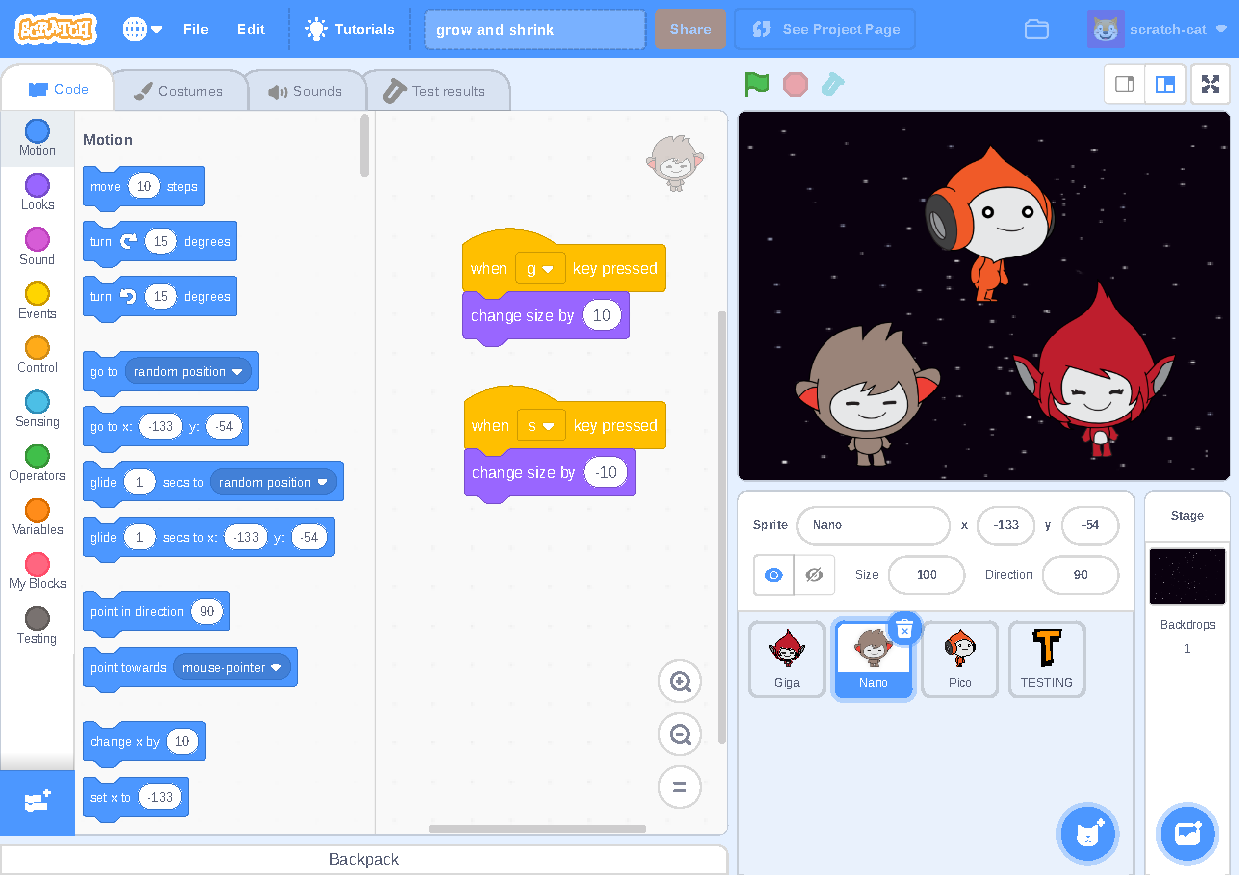
\includegraphics[width=\linewidth]{scratch-itch/itch-grow-and-shrink-code}
    \end{wide}
    \caption{
        The \emph{Grow and shrink} exercise.
        A correct implementation of the exercise for the sprite \texttt{Nano} is seen here.
    }
    \label{fig:itch-grow-shrink-code}
\end{figure}

To illustrate Itch with a concrete example, we will use one exercise as a running example: the \emph{Grow and shrink} exercise (\cref{fig:itch-grow-shrink-code}).
In this exercise, there are three sprites: each sprite must grow if the \keys{g} key is pressed and must shrink if the \keys{s} key is pressed.
To test this exercise, we design a test suite that will verify the behaviour of the sprites (\cref{lst:grow-and-shrink-during}).
This test suite will:

\begin{enumerate}
    \item Save the existing size of the sprites.
    \item Press the key that we are testing.
    \item Verify that the new size of the sprite is larger or smaller than the previously saved size.
    \item Save the new size as the existing size for the next test.
\end{enumerate}

\begin{listing}
    \begin{minted}{javascript}
function duringExecution(e) {
  const runtime = e.vm.runtime;
  // Save the original sizes of the sprites.
  const oldSize = {
    "Giga": runtime.getSpriteTargetByName("Giga").size,
    "Pico": runtime.getSpriteTargetByName("Pico").size,
    "Nano": runtime.getSpriteTargetByName("Nano").size
  }
  e.scheduler
    // Execute 4 events after each other.
   .forEach([1, 2, 3, 4], (prev) => {
     return prev.pressKey('g').log(() => {
       e.out.group("Test if sprites get bigger", () => {
         for (const sprite in oldSize) {
           const newSize = runtime.getSpriteTargetByName(sprite).size;
           e.out.test(`${sprite} got bigger`)
            .expect(newSize > oldSize[sprite])
            .toBe(true);
           // Save the new size as the old one.
           oldSize[sprite] = newSize;
         }
       })
     });
   }).forEach([1, 2, 3, 4], (prev) => {
    return prev.pressKey('s').log(() => {
      e.out.group("Test if sprites get smaller", () => {
        for (const sprite in oldSize) {
          const newSize = runtime.getSpriteTargetByName(sprite).size;
          e.out.test(`${sprite} got smaller`)
           .expect(newSize < oldSize[sprite])
           .toBe(true);
          oldSize[sprite] = newSize;
        }
      })
    });
  })
   .end();
}
    \end{minted}
    \caption{The complete Itch test suite for the \emph{Grow and shrink} exercise.}
    \label{lst:grow-and-shrink-during}
\end{listing}

\section{Test suites}\label{sec:itch-test-suites}

Test suites for Itch are written in JavaScript.
A test suite for Itch is split into three consecutive phases:

\begin{enumerate}
    \item The \term{before execution} phase, which is run before the execution of the Scratch project.
    \item The \term{during execution} phase, where the test suite controls the Scratch project and simulates user interaction.
    \item The \term{after execution} phase, where tests are run on the log, which was collected during the previous phase.
\end{enumerate}

All phases are optional: it is perfectly valid to not have a before execution, or only a before execution, depending on the types of tests that need to be run.
They are implemented with ``magic'' functions: these have a fixed signature (name and arguments) and will be called in the relevant phases (\cref{lst:itch-test-suite-skeleton}).

\begin{listing}
    \begin{minted}{javascript}
/** @param {Evaluation} e */
function beforeExecution(e) {
    // Tests go here
}

/** @param {Evaluation} e */
function duringExecution(e) {
    // Tests go here
}

/** @param {Evaluation} e */
function afterExecution(e) {
    // Tests go here
}
    \end{minted}
    \caption[]{
        A skeleton of a test suite for Itch that shows the three phases.
        Each phase is implemented as a separate function that will be called at the appropriate time by Itch.
        The argument to these functions is an instance of the \mintinline{javascript}{Evaluation} class, which provides various methods to help with testing, such as the test structure, assertion functions, etc.
    }
    \label{lst:itch-test-suite-skeleton}
\end{listing}

Broadly, the tests can also be split according to their type: there are \term{static tests} and \term{dynamic tests}.
Static tests do not require execution of the Scratch project.
They are generally easier to write and faster to execute, but are severely limited in what they can test.
Assessing whether a project uses a certain block (e.g.\ a loop block) somewhere in the project is typically done with static tests.
Assessing whether an existing sprite (e.g.\ blocks that are provided in the starter project) was not modified is also done with static tests.
Static tests can be done completely in the before execution phase.

Checking more high-level goals, such as ``Does the sprite move when clicked?'', is more challenging with static tests.
At least, without severely limiting the accepted solutions.
For example, there are multiple ways to implement a sprite that moves when clicked, and a good behavioural test needs to accept all implementations.
For these kinds of tests, dynamic tests can be used, which require the project to be executed.
Dynamic tests often require both the during and the after execution phases.
In the during execution phase, user interaction is simulated and the behaviour is captured.
This captured behaviour can then be inspected in the after execution phase to see if the actual behaviour matches with the required behaviour.

Testing can also be done in the during execution phase, for example, after a user action has been performed.
While this makes some test suites easier (like the one in \cref{lst:grow-and-shrink-during}), it does require attention to the parallel nature of Scratch.
If multiple tests are run in parallel, the output can be garbled.

\subsection{Structure of a test suite}\label{subsec:structure-of-a-test-suite2}

A test suite consists of a hierarchical structure of groups and tests, which can be nested.
A test is a check on some requirement or property of the exercise.
It can be correct or wrong and can contain feedback for both cases.
Additionally, a test also has a name and can include additional information, such as value comparisons, messages, etc.

Structure is added by grouping the tests.
Groups can be nested, so groups inside groups etc.\ are possible.
While there is no hard limit, we recommend not going deeper than three levels in most cases (the user interface that displays the feedback can also impose limits).
Groups are used for more than just structure.
They also support a notion of visibility, with three modes:

\begin{description}
    \item[Visible] The group is expanded (the group and all its children are visible).
    \item[Hidden] The group is completely hidden unless one of the tests in the group fails.
    \item[Summary] The group is collapsed by default, and a summary is shown unless one of the tests fails (in which case the group expands).
\end{description}

\begin{listing}
    \centering
    \begin{minted}{javascript}
        e.group.group('Tests for sprite A', () => {
          e.group
            .test('Sprite A does stuff right')
            .feedback({
              correct: 'Good job, sprite A does get stuff right!',
              wrong: 'Oh no, sprite A does not get it right.',
            })
           .expect('some value')
           .toBe('another value');
        });
    \end{minted}
    \caption{An example showing how the test suites are structured using groups and tests.}\label{lst:itch-test-suite-structure}
\end{listing}

Groups and tests in the JavaScript test suites are inspired by the Jest testing framework.\footnote{\url{https://jestjs.io/}}
The two relevant methods, \mintinline{javascript}{group} and \mintinline{javascript}{test} are available on the \mintinline{javascript}{Evaluation.group} property passed to the test suite.
\Cref{lst:itch-test-suite-structure} shows an example of this, containing a single test.
\marginnote{Maintainging backward compatibility is one of the downsides of using software in production.}
The double \mintinline{javascript}{group.group} is not a typo but needed for backward compatibility with older test suites.
The test, as written in the example, will always fail, since it expects the string \mintinline{javascript}{"some value"} to be equal to \mintinline{javascript}{"another value"}.
The \mintinline{javascript}{expect}/\mintinline{javascript}{toBe} notation specifically will be familiar to Jest users.

Groups can be given just a name, as in the example, but it is also possible to provide more structured data.
For example, it is possible to link a group to a certain sprite.
This information is also provided in the generated feedback, which means the platform responsible for showing the feedback can show an image of the sprite with the group.

More details on how this structure is reflected in the generated feedback can be found in \cref{sec:format-of-the-generated-feedback}.
Other possible metadata includes the visibility, a summary (used if the group's visibility is set to summary), some tags (which allows tagging groups with arbitrary strings), and an option to ignore wrong tests.
This last option means that if a test fails, it will be ignored completely and will not be outputted in the generated feedback.
This can be useful in cases where there are multiple possibilities: this allows trying each possibility until a passed test is found.

\subsection{Before execution}\label{subsec:before-execution}

The before execution phase allows for executing static tests.
Itch provides access to representations of two projects: the submission, created by the students, and the starter project, which is the project the students started with.

Access to both projects provides an easy way to assess whether the students modified some sprites or blocks in their submission.
Itch provides helpers to ensure that students only modified certain sprites, or only certain code within sprites.
While this does limit the students in their ability to creatively modify the project, it makes behavioural tests for complex projects easier.
By limiting where the students are allowed to modify blocks, later tests can rely on certain functionality or sprites being available and working.
For example, if the project contains blocks that check if a sprite touches another sprite, these can be relied on.

This functionality of checking a set of predefined blocks and sprites is exposed with the function \mintinline{javascript}{Itch.checkPredefinedBlocks} to test suite authors.
For example:

\begin{minted}{javascript}
    Itch.checkPredefinedBlocks({
      spriteConfig: {
        SpriteA: script(whenIReceive('Start'), setEffectTo('ghost', 0)),
        SpriteB: {
          pattern: script(whenIReceive('Start'), setEffectTo('ghost', 0)),
          allowedBlocks: [forever()],
          allowAdditionalScripts: true,
        },
      },
      debug: false,
    }, e);
\end{minted}

The example above contains tests for two sprites.
All other sprites must be unchanged.

For the sprite \texttt{SpriteA}, students are allowed to change, add, or remove blocks in the script starting with the two blocks \scratchinline{\blockinit{when I receive \selectmenu{Start}}} and \scratchinline{\blocklook{set \selectmenu{ghost} effect to \ovalnum{0}}}.
Students are allowed to change blocks after these two predefined blocks.

The second sprite, \texttt{SpriteB}, allows modifications to scripts starting with the same blocks, but it uses the full version of the config object.
With the full version, it is also possible to specify if additional scripts are allowed and limit the blocks they can use.
In this example, only the \scratchinline{\blockinfloop{forever}{\blockspace[0.2]}} block can be used (so this is not a useful test).
Finally, additional scripts (thus new ones created by the students) are also allowed.
These are free of restrictions: the check for allowed blocks does not apply.

\begin{listing}
    \begin{wide}
        \begin{sublisting}{0.49\linewidth}
            \begin{scratch}[scale=0.7]
                \blockinit{when I receive \selectmenu{Start}}
                \blocklook{set \selectmenu{ghost} effect to \ovalnum{0}}
                \blockrepeat{repeat \ovalnum{15}}
                {
                    \blocklook{change size by \ovalnum{3}}
                    \blockmove{change y by \ovalnum{-2}}
                }
                \blockrepeat{repeat \ovalnum{15}}
                {
                    \blocklook{change \selectmenu{ghost} effect by \ovalnum{5}}
                    \blockmove{change size by \ovalnum{3}}
                }
                \blocklook{hide}

            \end{scratch}
            \caption{A script in Scratch.}
        \end{sublisting}
        \begin{sublisting}{0.5\linewidth}
            \begin{minted}{javascript}
            script(
              whenIReceive('Start'),
              setEffectTo('ghost', 0),
              repeat(15, script(
                changeSizeBy(3),
                changeYBy(-2)
              )),
              repeat(20,script(
                changeEffectBy('ghost', 5),
                changeSizeBy(3)
              )),
              hide(),
            );
            \end{minted}
            \caption{The equivalent in JavaScript.}
        \end{sublisting}
    \end{wide}
    \caption{An example of how a Scratch program can be represented using the abstractions provided by Itch.}\label{lst:itch-block-abstraction}
\end{listing}

Itch also includes an abstraction to represent Scratch blocks in JavaScript, as used in the example above.
For each Scratch block, a corresponding function exists (see an example in \cref{lst:itch-block-abstraction}).

The functions representing blocks can also be used to construct block patterns.
Two additional functions are provided for patterns.
The first is \mintinline{javascript}{anything()}, which can be used in any location (as a block or value) and matches any block or value.
The reverse, \mintinline{javascript}{nothing()}, matches no block or value.
It can be useful to ensure that a script terminates (i.e.\ that there are no more blocks afterwards).
Additionally, an array of blocks or patterns can also be used in most places.
This represents a choice: it will match any of the patterns in the array.

For example, consider the following pattern:

\begin{minted}{javascript}
    repeat([15, 30], script(changeSizeBy(any()), never()))
\end{minted}

It will match a \scratchinline{\blockrepeat{repeat \ovalnum{}}{\blockspace[0.2]}} block that repeats 15 or 30 times, with a body with exactly one block, \scratchinline{\blocklook{change size by \ovalnum{}}}, whose argument can be anything.

Since scripts form a tree of blocks, there are also helpers to match and test against a script of blocks.
This supports error messages for each block (meaning they each show up as a failed assertion in the feedback).

\subsection{During execution}\label{subsec:during-execution}

\begin{listing}
    \begin{minted}{javascript}
        /** @param {Evaluation} e */
        function duringExecution(e) {
          e.scheduler
           .greenFlag(true)
           .wait(800)
           .pressKey('s')
           .end();
        }
    \end{minted}
    \caption{An example of the during execution phase where the scheduler is used to first press the green flag, wait \qty{800}{\milli\second}, press the \keys{s} key, and finally end execution.}\label{lst:itch-scheduler-example}
\end{listing}

The during execution phase is actually run just before the project is executed by Itch.
The main purpose of this phase is to use the \mintinline{javascript}{e.scheduler} (an instance of the \mintinline{javascript}{Scheduler} class) to schedule the execution of the project.
Using the scheduler, the test suite must specify how the project should be executed.
This includes starting execution, stopping execution, manipulating the virtual machine, and simulating user interaction, like clicking, key presses, input, and so on.
\Cref{lst:itch-scheduler-example} shows a minimal example of a schedule where the green flag is pressed, \qty{800}{\milli\second} must pass, and finally the \keys{s} key is pressed.

The scheduler receives a set of actions to perform.
Each next action is executed after the previous one has been scheduled or completed.
Because Scratch is a highly concurrent language, the scheduler also supports this.
First, most actions support a synchronous and asynchronous variant.
In the asynchronous variant, the action is executed and immediately finished.
For example, the action to press the green flag is almost instant: the green flag is pressed in the virtual machine, and the action is complete.

The synchronous actions will only finish after all activated scripts in Scratch have terminated.
For example, the action to press the green flag will wait on all scripts with the hat block \scratchinline{\blockinit{when \greenflag clicked}} are done executing.
Of course, there are scenarios where this is not possible.
If one of the scripts contains an infinite loop, the next scheduled action would never be performed, as the script will never end.

Since the project that is run comes from students with unknown code, synchronous actions also support a timeout.
After this time has passed, a failed assertion will be added to the generated feedback, and the scheduler will continue.

Every action in the scheduler returns the last scheduled action: this return value can be used to schedule the next action after the previous one.
To create a non-linear schedule (e.g.\ multiple actions are performed simultaneously), there are a few options.
First, the return value of one of the previous actions can be used multiple times to schedule new actions.
All of these will be run in parallel.

\begin{figure}
    \begin{subfigure}{0.49\linewidth}
        \centering
        \begin{minted}{javascript}
            const s = e.scheduler.wait(500);

            // Schedule actions L1-4
            s.forEach([1, 2, 3, 4], (p) => {
                return p.wait(500);
            });

            // Schedule actions N1-4
            s.forEach([1, 2, 3, 4], (p) => {
                p.wait(500);
                return p;
            });
        \end{minted}
    \end{subfigure}
    \begin{subfigure}{0.49\linewidth}
        \centering
        \includestandalone{scratch-itch/itch-scheduler}
    \end{subfigure}
    \caption{
        The code for the scheduler (left) and the resulting schedule of actions (right).
        The start of an action is shown with a circle.
        After the start action S, the L and N actions are scheduled at the same time.
        However, the L actions return the new action in the function, meaning L1-4 will run sequentially.
        The code for the N actions returns the original action, meaning N1-4 will run concurrently.
        Since both N1 and L1 are scheduled on the same action S, the actions L1 and N1-4 will all run concurrently.
    }
    \label{fig:itch-scheduler-schedule}
\end{figure}

Another option is to use the method \mintinline{javascript}{forEach}: this is an implementation of the ``fold'' function on the scheduler events.
By deciding what action is used as the accumulator, either a linear (by returning the new action) or non-linear schedule (by returning the existing action) can be created.
\Cref{fig:itch-scheduler-schedule} shows an example of this.
By returning the new action, each action L1-4 will be performed in succession.
By returning the original action, the N1-4 actions will all be scheduled at the same time.
Since both L1 and N1 are scheduled on the same starting action S, they will also run in parallel.

While most actions are equivalent to their counter-parts in Scratch (like clicking a sprite, pressing a key, etc.), the wait action has more features.
In addition to waiting a set amount of time (like in the example), the wait action can also wait on the fulfillment of a certain condition.
The wait condition can be either waiting on a certain broadcast being sent, or a sprite fulfilling some condition.
The possible sprite conditions are moving, reaching a certain position, touching another sprite, no longer touching another sprite, touching the edge, and touching the mouse.
These conditions are added as needed, so with use, we envision more conditions being added.

A final special action is the \mintinline{javascript}{log} action.
This action saves the current state in the log (\cref{subsec:after-execution}) and executes a custom function at that time.
This action is intended to mark certain events in the log but can also be used to execute a test during the execution of the project, instead of beforehand or afterwards.
While the test is executed during the execution, it also has access to snapshots and events that have already taken place.

\subsection{After execution}\label{subsec:after-execution}

\begin{listing}
    \begin{minted}{javascript}
        function duringExecution(e) {
          // Schedule pressing each key four times in succession.
          e.scheduler
           .forEach([1, 2, 3, 4], (prev) => prev.pressKey('g'))
           .forEach([1, 2, 3, 4], (prev) => prev.pressKey('s'))
           .end();
        }

        function afterExecution(e) {
          const sprites = ["Giga", "Pico", "Nano"];

          // Get the events for the g key presses.
          const gPresses = e.log.events.filter((e) => e.type === 'key' && e.data.key === 'g');
          for (const event of gPresses) {
            e.out.group("Test if sprites get bigger", () => {
              for (const name of sprites) {
                // Get the sprite from the snapshot before the key press.
                const before = event.previous.sprite(name);
                // Get the sprite from the snapshot after the key press.
                const after = event.next.sprite(name);

                e.out.test(`${name} got bigger`)
                 .expect(after.size > before.size)
                 .toBe(true);
              }
            });
          }

          const sPresses = e.log.events.filter((e) => e.type === 'key' && e.data.key === 's');
          for (const event of sPresses) {
            e.out.group("Test if sprites get smaller", () => {
              for (const name of sprites) {
                const before = event.previous.sprite(name);
                const after = event.next.sprite(name);

                e.out.test(`${name} got smaller`)
                 .expect(after.size < before.size)
                 .toBe(true);
              }
            });
          }
        }
    \end{minted}
    \caption{
        Alternative test suite for the \emph{Grow and shrink} exercise.
        In contrast to \cref{lst:grow-and-shrink-during}, this test suite only schedules the key presses in the during execution phase.
        All tests are performed in the after execution phase using the log.
    }
    \label{lst:grow-and-shrink-after}
\end{listing}

Itch uses the scheduler from the during execution phase to execute the submission.
During the execution, a log is constructed of the execution.
This is done by hand (using the \mintinline{javascript}{log} scheduler action) and automatically at interesting points.
The log consists of snapshots (which are taken every time something changes in the virtual machine) and events (which denote interesting snapshots).
For example, every action in the scheduler is saved as an event, meaning there is a snapshot before the action and after the action has been completed.

Returning to the \emph{Grow and shrink} exercise, \cref{lst:grow-and-shrink-after} shows an alternative test suite (compared to \cref{lst:grow-and-shrink-during}).
In the during execution phase, only the key presses are scheduled.
Afterwards, in the after execution phase, the log is used to perform the tests.
For each key press, the corresponding event in the log is looked up.
Each of these events provides before and after snapshots, which are then used to determine if sprites correctly change in size.

\section{Evaluating projects}\label{sec:itch-evaluating-projects}

The evaluation of a submission goes through the following process:

\begin{enumerate}
    \item The submission, the starter project, and the test suite are made available.
    \item Itch loads both projects, and runs the before execution phase.
    While the starter project is available in all phases, it is only intended to be used in the before execution phase.
    \item If the before execution phase does not result in an error, Itch initializes the virtual machine, inserts hooks for the log, and loads the submission into the virtual machine.
    \item The during execution phase is run, and the scheduled actions are read from the test suite.
    The during execution phase is used to create a schedule of user actions using the scheduler.
    It does not run the schedule itself.
    \item Itch starts the virtual machine and executes the scheduled actions.
    While executing, the logs are captured.
    \item If the execution does not result in an error, Itch shuts down the virtual machine, and runs the after execution phase.
    \item All feedback is sent to the output.
    The output is a callback function that can be provided when starting Itch, or the default function is used, which prints the feedback on standard output.
\end{enumerate}

Scratch 3.0 is built using browser technologies and has to be run in the browser.
While the virtual machine is pure JavaScript and could thus run without a browser, the renderer is not: it uses the HTML canvas and WebGL technologies.
The renderer is used to calculate things like sprite collisions and checking if sprites touch certain colours.
While it is theoretically possible to create a renderer that does not use WebGL, this would be a big undertaking and imply a big maintenance burden.
The re-implemented renderer will have to be kept up to date with the upstream one and replicate all behaviour exactly.

Itch consists of two JavaScript packages, which is a reflection of the two ways to run Itch:

\begin{itemize}
    \item As a library in the browser.
    This is useful for contexts where there already is a browser, e.g.\ running Itch along the Scratch environment on the device of the student for client-side testing.
    This is implemented by the first JavaScript package, the core package.
    \item As a command line tool.
    This is for cases where Itch runs as a service in the backend, e.g.\ to check submissions after students are done.
    This is implemented in the second JavaScript package, the runner package.
    This package wraps around the core package to launch the browser instance and load the various dependencies (it thus runs the core package, which is where it gets its name).
\end{itemize}

\subsection{Running Itch as a library}\label{subsec:running-itch-as-a-library}

\begin{listing}
    \begin{minted}{typescript}
        export interface EvalConfig {
          /** The submission sb3 data. */
          submission: ArrayBuffer;
          /** The starter project sb3 file. */
          template: ArrayBuffer;
          /** If the output should be partial or full. */
          fullFormat: boolean;
          /* The canvas for the renderer. */
          canvas: HTMLCanvasElement;
          /** The test suite to use. */
          testplan: string | TestplanSource;
          /** Callback for the results. */
          callback: OutputHandler;
          /** The language of the exercise. */
          language: string;
        }

        /** Run the judge. */
        export async function run(config: EvalConfig): Promise<void>;
    \end{minted}
    \caption{The exposed interface to run Itch. It consists of one function and a configuration object.}\label{lst:itch-library-interface}
\end{listing}

When running Itch as a library, the core package must be loaded into the browser, in addition to having the Scratch dependencies (the virtual machine, etc.) available.
The exposed interface to run Itch is limited to one function and a configuration object (\cref{lst:itch-library-interface}).
Most of the options are self-explanatory, and the output format option is explained in \cref{sec:format-of-the-generated-feedback}.

\subsection{Running Itch as a command line tool}\label{subsec:running-itch-as-a-command-line-tool}

\begin{figure}
    \begin{wide}
        \includestandalone[width=\linewidth]{scratch-itch/itch-sequence-diagram}
    \end{wide}
    \caption{Sequence diagram showing the process of evaluating a project with Itch. When run as a library, there is no Itch core or Puppeteer.}
    \label{fig:itch-sequence-diagram}
\end{figure}

When there is no existing browser instance available, Itch provides a command line interface.
\marginnote{A headless browser is a full browser, but without user interface.}
In this mode, Itch will run a headless browser, load the projects and test suites, run the judge, and finally collect the results from the browser.

\Cref{fig:itch-sequence-diagram} shows the complete process.
First, the runner package launches a Puppeteer instance (the headless browser).
When ready, the various dependencies are loaded into the Puppeteer instance (these are the Itch core package, the Scratch dependencies, the test suite, the submission, and the starter project).
The runner package will then run a special script that calls Itch as it would be used as a library: the \mintinline{typescript}{run(config)} function is called.
Then, the same process happens as when using Itch as a library.
First, the projects (submission and starter) are parsed.
The phases are then executed, with the before and during execution phase going first.
The during execution phase results in a schedule, which is then run.
The virtual machine is started and runs the projects with the scheduled actions.
Finally, the after execution phase is run, with the log from the previous phase.

\subsection{Performance considerations}\label{subsec:performance-considerations}

Reducing the time students spend waiting on feedback is essential for providing a good user experience with software testing, especially in educational software testing~\autocite{sarsaSpeedingAutomatedAssessment2022}.
One difficulty in providing fast feedback on Scratch code is that blocks that wait are commonly used.
However, these wait times pose a hard lower limit on the duration of the evaluation of a Scratch project.
For example, if a project has a wait block of 2 seconds, the evaluation time of that project can never be less than 2 seconds (and will be higher in practice, since the whole evaluation process also adds overhead).
Such wait blocks can quickly add up.

As a solution for this problem, Itch provides test suites with the ability to set an ``acceleration factor'': this factor indicates the speedup for all time-based data, both in the project and in the test suite.
For example, if the acceleration factor is 2, the wait time in wait blocks will be halved, as will wait times in the scheduler.
The acceleration factor can, however, be flaky with high values: we do not recommend a factor higher than 5.
If it is expected that, for example, wait blocks are used for synchronization of two sprites, the acceleration factor can cause issues, as it does not speed up general execution.
For example, if a wait block has a value timed to wait as long as the execution of another script with five blocks takes, the acceleration factor will cause the wait block to stop waiting early.

Itch also provides the test suite with the possibility to enable Scratch's built-in turbo mode.
In this mode, execution is done faster (how much depends on the project).
Together with the acceleration factor, these techniques can significantly speed up the evaluation.

\section{Format of the generated feedback}\label{sec:format-of-the-generated-feedback}

The format of the generated feedback is in structure similar to the structure of the tests in the test suite (\cref{subsec:structure-of-a-test-suite}).
The three levels of the feedback are:

\begin{enumerate}
    \item \term{Judgement}: the top-level object of the feedback.
    \item \term{Group}: contains one or more tests or subgroups (equivalent to a group from the test suite).
    Each group has the same options as in the test suite (e.g.\ for its visibility, a linked sprite).
    \item \term{Test}: one condition or requirement that is evaluated (equivalent to a test from the test suite).
\end{enumerate}

Itch uses a callback function to process feedback and has two modes.
In partial mode, the callback is called whenever feedback is available.
Full mode means all feedback is collected and the callback is called once with the collected feedback.

\begin{listing}
    \begin{wide}
        \begin{minted}{json}
        {"command": "start-judgement", "version": 2}
        {"command": "start-group", "name": "Check on existing code", "visibility": "summary"}
        {"command": "start-group", "name": "Stage", "sprite": "Stage", "visibility": "summary"}
        {"command": "start-test", "name": "Sprite exists"}
        {"command": "close-test", "feedback": "The sprite exists", "status": "correct"}
        {"command": "close-group"}
        {"command": "close-group"}
        {"command": "close-judgement"}
        \end{minted}
    \end{wide}
    \caption{Example of the output generated by Itch for a test suite with two nested groups, with one test. Note the similarity to \cref{lst:tested-output-example}.}\label{lst:itch-output-example-partial}
\end{listing}

When running Itch on the command line, a default callback function is used.
This default will send all feedback to standard output in a format similar to the Dodona feedback format used by TESTed (\cref{subsec:dodona-output}).
The feedback is printed as newline-delimited JSON, meaning JSON objects are separated by a newline, and each line is a valid JSON object.
\Cref{lst:itch-output-example-partial} gives an example of this format.
In partial mode, the structure of the feedback is indicated by commands, with \texttt{start} commands to begin a new level in the hierarchy and \texttt{close} commands to finish a level.
The full mode is similar, but there is only a single big JSON object that represents a nested tree of the same feedback.

\section{Itch in practice}\label{sec:itch-evaluation}

In this section, we discuss the use of Itch in educational practice and discuss insights from creating test suites for Scratch exercises.

\subsection{Capabilities of the testing framework}\label{subsec:capabilities-of-the-testing-framework}

The initial development of Itch used a set of 13 Scratch exercises from the 2017 edition of the Flemish Programming Contest (\textdutch{\emph{Vlaamse Programmeerwedstrijd}}).
The Scratch exercises were used in a special category for students aged 10 to 12.
This category was a one-time event organized by the local organizer as a side-event for the Programming Contest, which normally focuses on text-based programming languages.
It is worth mentioning that this event used human judges to assess whether the children had successfully completed an assignment.
An example of one such exercise is given in \cref{ch:task-description-of-the-flemisch-programming-contest}.
This was the case as there were no Scratch testing frameworks at the time that could automate this assessment: as a result, the exercises were not created with automated assessment in mind.

These 13 exercises were used as a reference for the initial feature set and capabilities of Itch.
The exercises can be classified into five groups, depending on their contents:

\begin{description}
    \item[Speaking] Sprites speak, think, or ask questions (five exercises).
    \item[Moving] Sprites move around (three exercises).
    \item[Costumes] Sprites change costumes, often to emulate animation (three exercises).
    \item[Games] Interactive games that require user input (one exercise).
    \item[Drawing] The \emph{Pen} extension is used to draw on the canvas (three exercises).
\end{description}

Note that the exercises do not sum up to 13: two exercises are both in the moving and costumes category, since they do both.

For 12 of the 13 exercises, an Itch test suite was created that tested the submissions sufficiently that it would have been usable in the programming contest.
The remaining exercise was not testable due to its open-ended nature.
The task description is, in summary, ``draw a house''.
Which leads to a vast variety of houses as solutions.
Besides introducing some computer vision framework to detect houses (which would be technically possible in Itch), this is not easily testable.

These exercises were all tested with dynamic tests, meaning they test the behaviour of the submission.
The exercises of CodeCosmos (which are discussed in \cref{subsec:itch-in-educational-practice}) are often longer interactive games.
Due to their complex nature, static testing was sometimes needed (which is discussed in \cref{subsec:creating-test-suites-for-scratch-exercises}).

\subsection{Itch in educational practice}\label{subsec:itch-in-educational-practice}

The use of Itch in educational practice has done mainly with our commercial partner, CodeCosmos.
CodeCosmos provides the platform in which Itch is integrated.
The platform provides a variety of organizational tools, like classroom management.
It has its own hosted instance of the Scratch environment (similar to the MIT-hosted instance).
This instance has been modified to integrate with Itch.

On the platform, Itch is run server-side by a dedicated service.
The choice for server-side testing versus client-side testing was mainly motivated by making sure that students could not cheat by modifying the test suites or the results.
The platform will periodically (or when a button is pressed) send the current version of the submission to the server.
The backend will then look up the test suite and starter project and send these to the Itch service.
After testing has been completed, the results are returned to the platform where they are displayed to the students in an additional, custom tab in the Scratch environment.

There are two different ways in which the CodeCosmos programming exercises are used.
The first is as part of a ``teaching pack'', which is bought and used by schools.
These packs implement the ``attainment descriptors''\marginnote{Called \textenglish{eindtermen} in Dutch.}, which are documents that describe the learning objectives of the lessons and what skills students should possess after taking the courses.
Here, the teaching pack provides a full learning path for the students, with suitable exercises at each stage of the process.
The second way is as an extracurricular activity, where students either follow weekly lessons or join a ``coding camp'' for a few weeks in the summer.
In both cases, many of the same exercises are used, but the context in which they are used differs.

In total, there are 139 exercises with an Itch test suite.
In the period from March 3rd, 2023 until March 26th, 2024 (328 days), Itch evaluated \num{28144} submissions.
Of these submissions, \num{2713} (\qty{9.64}{\percent}) are evaluated as being correct, which means \qty{90.36}{\percent} of evaluated submissions are incorrect.
This is in line with our expectations: we allow students to submit as much as they want (and even automatically submit every so often) until the submission is correct.
This also allows for collecting information about the trajectory of students while solving an exercise but also provides more data for analysing the growth of students throughout a course.
Providing insights from this data to educators is one area of future work that is planned by CodeCosmos.

The submissions were made by \num{6496} unique users, with an average of \num{4.33} submissions per user.
The submissions have an average test count of \num{158}, (the exercises have a number of tests that range from a minimum of \num{2} and a maximum of \num{1292}).

Most of these exercises were conceived before introducing Itch, meaning Itch is capable of evaluating exercises as typically used by CodeCosmos.
The biggest change we made to the exercises was splitting the levels of the exercises into different Scratch projects.
However, coming up with a test suite for all of these exercises was a challenge, which is discussed next.

\subsection{How to assess Scratch projects}\label{subsec:how-to-evaluate-scratch-submissions}

The creators of Scratch have a well-known vision on how they intend Scratch to be used.
The Scratch team prefers not to use assignment-based learning~\autocite{resnickCodingCrossroads2020}.
As a specific example of this, they particularly do not support strict static tests on exercises.
For example, \citeauthor{resnickCodingCrossroads2020} state:

\begin{quotation}
    Too often, researchers and educators are adopting automated assessment tools that evaluate student programming projects only by analysing the code, without considering the project goals, content, design, interface, usability, or documentation.
    \marginnote{They are probably talking about Dr.\ Scratch here.}
    For example, many are using an online Scratch assessment tool that gives students a ``computational thinking score'' based on the assumption that code with more types of programming blocks is an indication of more advanced computational thinking.
    This form of assessment doesn't take into consideration what the student's program is intended to do, how well it accomplishes the student's goals, whether the code works as intended, whether people are able to interact with it, or how the student's thinking develops over a series of projects.
\end{quotation}

At the same time, using linters or other static analysis tools to detect code smells is considered beneficial for students~\autocite{hermansCodeSmellsHamper2016}.
However, in Itch, static analysis can also be used for automatic assessment by writing static tests.
While we share the sentiment of \citeauthor{resnickCodingCrossroads2020}, our experience with Scratch exercises and our collaboration with CodeCosmos has shown that such tests are often used, despite their disadvantages.
There are a few factors that contribute to this:

\begin{itemize}
    \item Exercises (especially in Scratch) that were not created with testability in mind are hard to properly test without resorting to static analysis of the code.
    \item Scratch projects, especially complex ones, are technically challenging to test within an acceptable time frame.
    We cannot spend minutes evaluating a single submission, as feedback must be provided quickly to students~\autocite{sarsaSpeedingAutomatedAssessment2022}.
    \item Educators want simple metrics to easily see if students have mastered some concept.
    For example, determining if a student has mastered the concepts of loops (or repetition in general) is challenging to do automatically.
    With a large number of students and time constraints, educators fall back on analysing blocks as a proxy for mastery~\autocite{combefisAutomatedCodeAssessment2022}.
\end{itemize}

This does not mean that static tests are of no use: with good and thoughtful static tests, an educator (and student) can be fairly certain that a submission marked as correct is effectively correct.
This can guide the educator to spend more time on submissions where their attention is warranted.
Similarly, a submission marked as wrong can also help pinpoint the problem to the student, without intervention from the educator.

However, as so eloquently stated by Edsger Dijkstra, ``Testing shows the presence, not the absence of bugs''.
Students might have solved the exercise in creative or innovative ways, which static tests fail to detect.
Similarly, they might have fooled the static tests into marking the submission as correct, even though it is not.
Therefore, we do not recommend using static tests to automatically grade submissions, at least not without verifying the results.

\subsection{Creating test suites for Scratch exercises}\label{subsec:creating-test-suites-for-scratch-exercises}

Itch does not use the same programming language for the test suites as the programming language of a submission: test suites for Scratch exercises are written in JavaScript.
\marginnote{Doing the same in Scratch would be much less ergonomic then doing it in JavaScript.}
This has advantages, as JavaScript is a general-purpose programming language, while Scratch is much more limited, but it also has disadvantages.

It is not uncommon for educators that use or create Scratch exercises to have no formal computer science background, nor experience with programming besides Scratch~\autocite{kimEnhancingTeachersICT2012,oliveiraIntroductionComputationalThinking2019}.
This is also the case at CodeCosmos, where teachers with an educational background design and create the exercises.
For the existing exercises, the educators designed the exercise and implemented the Scratch parts, while others (like the author of this dissertation) implemented the test suites.
However, it is our experience that authoring exercises is faster if the people designing the exercise have knowledge of the testing framework and implement the test suite themselves.
In \cref{sec:poke:-a-testing-framework-written-in-scratch}, we explore an experiment showing what a testing framework for Scratch with test suites in Scratch may look like.

\section{Writing test suites in Scratch}\label{sec:poke:-a-testing-framework-written-in-scratch}

As mentioned in the previous subsection, creating test suites in JavaScript for Scratch exercises can be challenging for educators without computer science background or experience.
To fill this gap, we have developed Poke: a prototype of a testing framework for Scratch implemented in Scratch itself.
This means that test suites are written with Scratch blocks, tests are executed in the Scratch environment, and the results are also shown in the Scratch environment.

For this prototype, our focus was twofold: ``Is it possible to create a testing framework for Scratch in Scratch?'' and ``If possible, which testing facilities should be present?''.
The answer to the first question is yes, and the remainder of this section discusses the details of Poke, along with answers for the second question.
These considerations include what blocks to provide, how tests should be run, etc.

\subsection{Introduction to Poke}\label{subsec:introduction-to-poke}

\begin{figure}
    \begin{wide}
        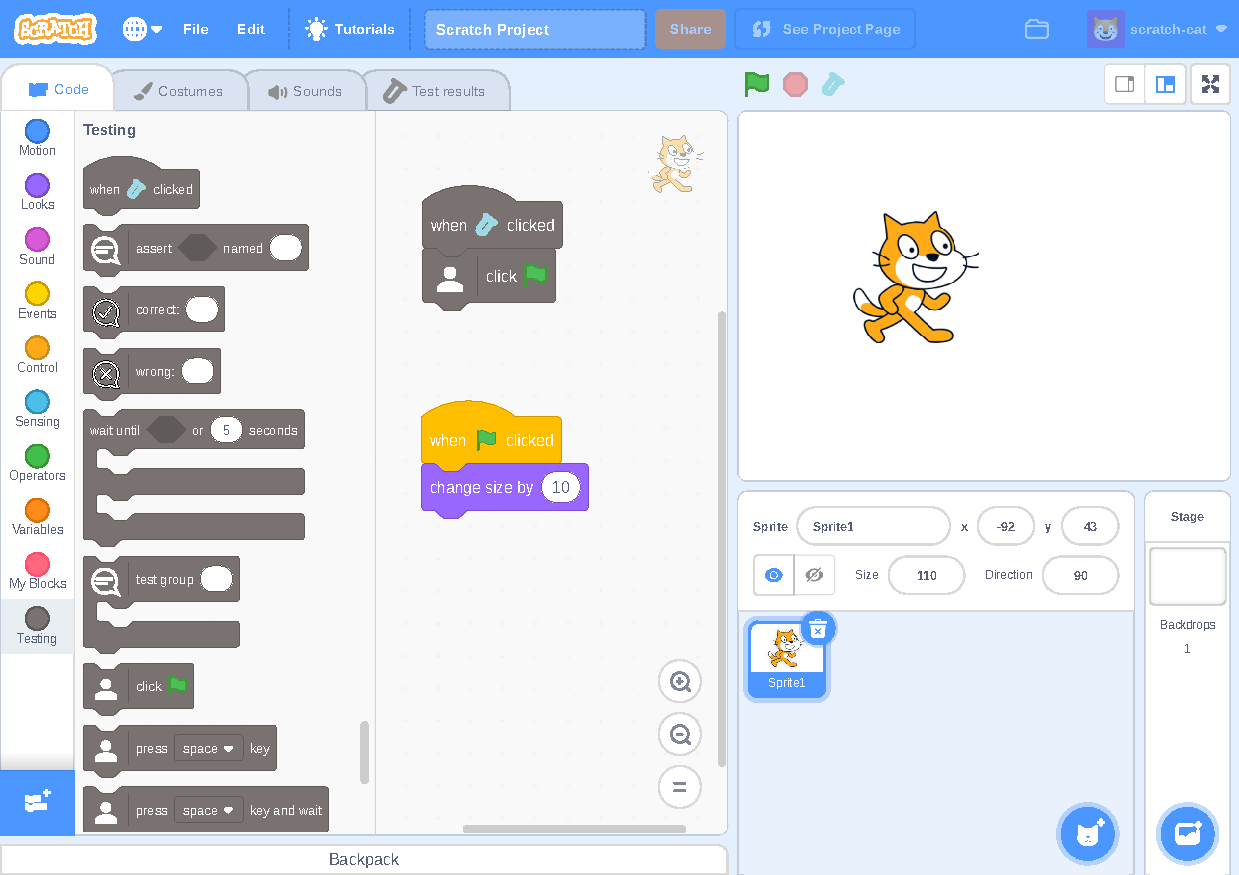
\includegraphics[width=\linewidth]{scratch-itch/poke-ui}
    \end{wide}
    \caption{The Scratch environment with the added Poke elements: the additional button next to green flag and stop buttons to start the tests, the additional tab to show test results, and the extension that provides the Poke blocks.}
    \label{fig:poke-ui}
\end{figure}

The user-facing part of the Poke software testing framework consists of three parts (\cref{fig:poke-ui}):

\begin{itemize}
    \item An additional button next to the green flag and stop button, which will run the tests.
    \item An extension to provide a set of blocks to write tests with.
    \item An additional tab in the Scratch environment that shows the test results once run.
\end{itemize}

\subsection{The Poke extension}\label{subsec:poke-provided-blocks}

Poke provides five categories of blocks: a hat block (\scratchinline{\blockpokehat{when \drawtesttube clicked}}, which starts the tests if the button is clicked), feedback blocks, user interaction blocks, observation blocks, and blocks to execute code in another sprite.

\subsubsection{Feedback blocks}

\begin{scratch}[scale=0.6]
    \blockpokegroup{\drawicon{\drawfeedback} test group \ovalnum{name}}{\blockspace[0.5]}
\end{scratch}

The structure of a test suite in Poke is identical to the structure in Itch (\cref{subsec:structure-of-a-test-suite2}): a test suite consists of groups, which can contain tests or other groups.
The block for creating groups is a C block that takes the name of the group as an argument.
The body of the block outputs its test results in the group.

\begin{varwidth}{0.40\linewidth}
    \begin{scratch}[scale=0.6]
        \blockpoke{\drawicon{\drawfeedback} assert \boolpokeempty[3em] named \ovalnum{feedback}}
    \end{scratch}
\end{varwidth}%
\hspace{1em}%
\begin{varwidth}{0.28\linewidth}
    \begin{scratch}[scale=0.6]
        \blockpoke{\drawicon{\drawfeedbackcorrect} correct: \ovalnum{feedback}}
    \end{scratch}
\end{varwidth}%
\hspace{1em}%
\begin{varwidth}{0.25\linewidth}
    \begin{scratch}[scale=0.6]
        \blockpoke{\drawicon{\drawfeedbackwrong} wrong: \ovalnum{feedback}}
    \end{scratch}
\end{varwidth}

For generating test results, there are three blocks, the main of which is the assertion block.
It takes a boolean value and a name.
The name is shown in the output, together with a status depending on the value of the boolean block.
There are also the correct and wrong blocks, which act as a test that always passes or always fails respectively.

\begin{scratch}[scale=0.6,else word={}]
    \blockpokedgroup{\drawicon{\drawfeedback} wait until \boolpokeempty[3em] or \ovalnum{} seconds}{\blockspace[0.5]}{\blockspace[0.5]}
\end{scratch}

A special block is the wait until or timeout block.
This block will wait until the condition evaluates to true or the specified number of seconds has passed.
If the condition evaluates to true within the time limit, the first slot is used, which will often contain a \scratchinline{\blockpoke{\drawicon{\drawfeedbackcorrect} correct: \ovalnum{}}} block.
Otherwise, the second slot is used, which will often contain a \scratchinline{\blockpoke{\drawicon{\drawfeedbackwrong} wrong: \ovalnum{}}} block.
The two slots can also contain other blocks.

\subsubsection{User interaction blocks}

\begin{varwidth}{0.20\linewidth}
    \begin{scratch}[scale=0.6]
        \blockpoke{\drawicon{\drawinteract} click \greenflag}
    \end{scratch}
\end{varwidth}%
\hspace{1em}%
\begin{varwidth}{0.28\linewidth}
    \begin{scratch}[scale=0.6]
        \blockpoke{\drawicon{\drawinteract} click \selectmenu{Sprite}}
    \end{scratch}
\end{varwidth}%
\hspace{1em}%
\begin{varwidth}{0.3\linewidth}
    \begin{scratch}[scale=0.6]
        \blockpoke{\drawicon{\drawinteract} click \selectmenu{Sprite} and wait}
    \end{scratch}
\end{varwidth}

\begin{varwidth}{0.5\linewidth}
    \begin{scratch}[scale=0.6]
        \blockpoke{\drawicon{\drawinteract} press \selectmenu{space} key}
    \end{scratch}
\end{varwidth}%
\hspace{1em}%
\begin{varwidth}{0.5\linewidth}
    \begin{scratch}[scale=0.6]
        \blockpoke{\drawicon{\drawinteract} press \selectmenu{space} key and wait}
    \end{scratch}
\end{varwidth}%

\begin{varwidth}{0.5\linewidth}
    \begin{scratch}[scale=0.6]
        \blockpoke{\drawicon{\drawinteract} move mouse to x: \ovalnum{} y: \ovalnum{}}
    \end{scratch}
\end{varwidth}%
\hspace{1em}%
\begin{varwidth}{0.5\linewidth}
    \begin{scratch}[scale=0.6]
        \blockpoke{\drawicon{\drawinteract} answer \ovalnum{answer text}}
    \end{scratch}
\end{varwidth}%

The user interaction blocks will simulate user interaction, similar to the scheduler in Itch (\cref{subsec:during-execution}).
Currently, there are blocks to click the green flag, click a sprite, move the mouse, press a key, and answer a question.
The block to click a sprite and the block to press a key also have a synchronous variant, which will wait until all activated scripts have finished, again similar to the synchronous/asynchronous actions in the scheduler from Itch.

\subsubsection{Observation blocks}

\begin{varwidth}{0.2\linewidth}
    \setscratch{scale=0.6}\ovalpoke{\drawicon{\drawobserve} snapshot}
\end{varwidth}%
\hspace{1em}%
\begin{varwidth}{0.5\linewidth}
    \setscratch{scale=0.6}\ovalpoke{\drawicon{\drawobserve} \selectmenu{property} of \selectmenu{Sprite} in \ovalnum{snapshot}}
\end{varwidth}%
\hspace{1em}%
\begin{varwidth}{0.3\linewidth}
    \setscratch{scale=0.6}\ovalpoke{\drawicon{\drawobserve} \selectmenu{property} in \ovalnum{snapshot}}
\end{varwidth}

The observation blocks are similar to sensing blocks from Scratch, as they allow the tests to save and query the environment.
A special sensing block (which also acts as a variable) reflects the current state of the virtual machine.
Test code can then save this state into a variable, making it available later.
Two more reporter blocks (one for sprite-specific properties and one for the stage) allow querying specific properties (of specific sprites) from the saved state (or the current state).

\subsubsection{Executing blocks in another sprite}

\begin{varwidth}{0.5\linewidth}
    \begin{scratch}[scale=0.6]
        \blockpokegroup{\drawicon{\drawsquarearrow} with \selectmenu{Sprite} do}{\blockspace[0.5]}{}
    \end{scratch}
\end{varwidth}%
\hspace{1em}%
\begin{varwidth}{0.5\linewidth}
    \begin{scratch}[scale=0.6]
        \blockpoke{\drawicon{\drawsquarearrow} add sprites to \selectmenu{list} where \boolpokeempty[3em]}
    \end{scratch}
\end{varwidth}%

While the test blocks can be placed in any sprite, it is our experience that the most convenient place is a dedicated sprite with only test code or in the stage if it does not have code itself.
However, this introduces an additional complication: how can the test sprite execute blocks in other sprites?
For example, the test sprite might want to move a certain sprite, which is not possible in vanilla Scratch.

To this end, Poke provides a C block, whose contents will be executed in the selected sprite.
Technically, this re-uses the broadcasting mechanism built into Scratch.
Behind the scenes, the following process happens:

\begin{enumerate}
    \item Before executing a test, Poke will generate a unique broadcast for each of these C blocks.
    \item The contents of the C block are copied to the sprite that will execute them.
    \item These copied blocks are placed under a hat block that will trigger when the generated broadcast is sent.
    \item The original blocks are replaced with a send broadcast block.
\end{enumerate}

When the virtual machine executes this code, it will send the broadcast, which will trigger the blocks in the correct sprite.
This happens transparently for the user: the copied blocks are not visible to the user, and special care has been taken to ensure that there are no performance issues.
For example, the blocks are only copied once (or when they are changed).

\subsection{Feedback in the Scratch environment}\label{subsec:feedback-in-the-scratch-environment}

% TODO: update Scratch environment?
% TODO: update icons to be svg...
\begin{figure}
    \begin{wide}
        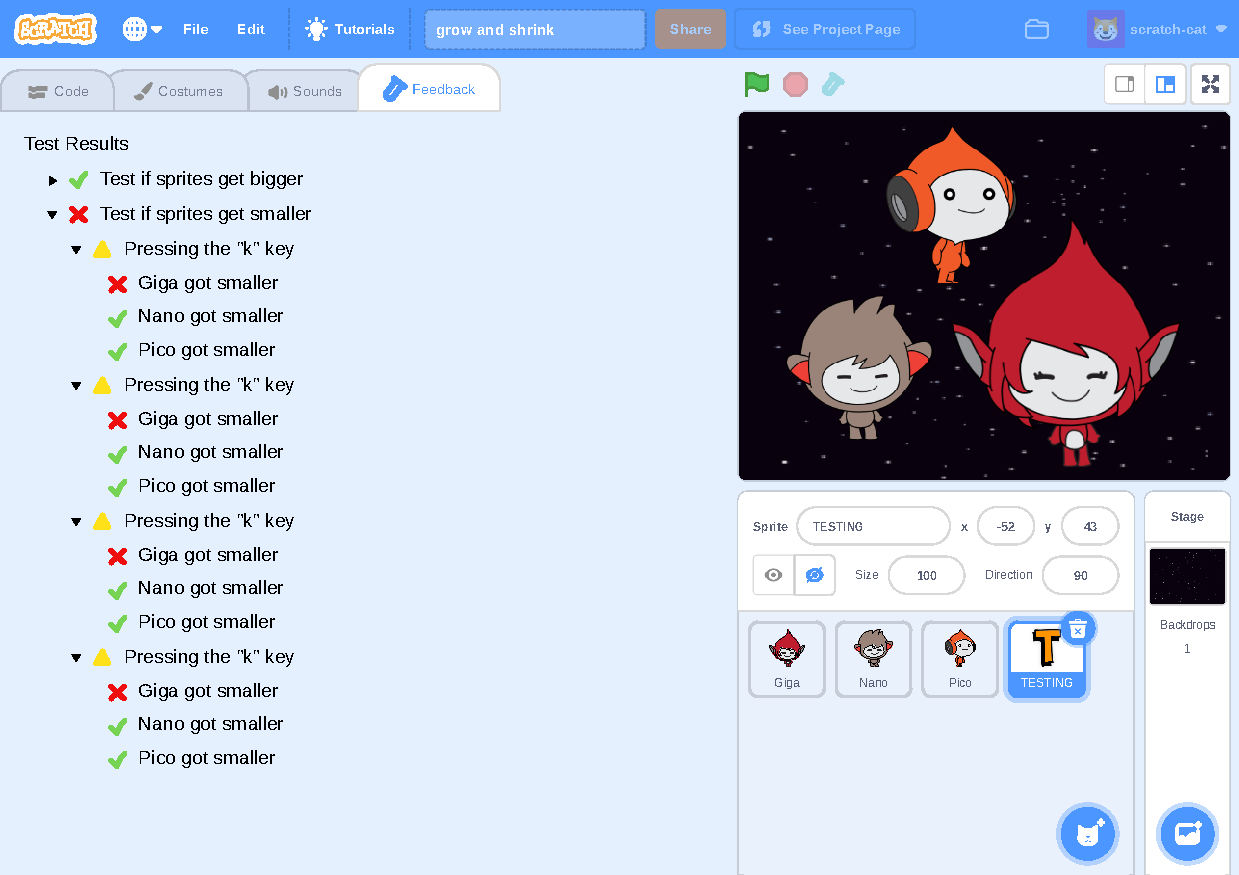
\includegraphics[width=\linewidth]{scratch-itch/scratch-poke-feedback}
    \end{wide}
    \caption{
        Feedback for the \emph{Grow and shrink} exercise.
        The submission's implementation contains an error: the sprite \texttt{Giga} does not implement the shrinking behaviour (with the \keys{s} key).
        In the feedback, there are two test groups: one for checking that sprites grow and one for checking that sprites shrink.
        In each of these groups, the relevant key is pressed four times and each sprite is checked.
        In the ``grow'' group, everything is correct (indicated by the green tick marks).
        As expected, the second group reports that some tests have failed (indicated by the yellow triangles).
        Two of the subgroups are open: while the tests for \texttt{Nano} and \texttt{Pico} were correct, the one for \texttt{Giga} failed as expected (indicated by red crosses).
        \Cref{lst:poke-grow-and-shrink} shows the test suite that generated this feedback.
    }
    \label{fig:poke-feedback-result}
\end{figure}

For this prototype, showing feedback to students was not a priority.
As such, the feedback is shown in a rudimentary interface, which shows the feedback in a tree format (\cref{fig:poke-feedback-result}).
While usable, it is not the most intuitive layout, especially considering the target demographic of Scratch users.

\subsection{Comparing Poke to Itch}\label{subsec:comparing-poke-to-itch}

To verify that Poke is usable as a testing framework, we compared it to the set of Scratch problems from the Flemish Programming Contest (\cref{subsec:capabilities-of-the-testing-framework}) that were testable by Itch.

Three of the exercises could not be tested with Poke, but this was expected.
Poke does not support extensions at the moment, and these exercises use the \textit{Pen} extension.
One of these three exercises would not be testable anyway, for the same reason Itch could not test it: drawing a house is an open-ended exercise.
The other exercises could be tested with Poke if the \textit{Pen} extension were supported.

\Cref{lst:poke-grow-and-shrink} shows the Poke test suite for the \emph{Grow and shrink} exercise.
For comparison, the Itch test suite for the same exercise is \cref{lst:grow-and-shrink-during}.

\begin{listing}
    \begin{wide}
        \begin{scratch}[scale=0.6]
            \blockpokehat{when \drawtesttube clicked}
            \blockpokegroup{\drawicon{\drawfeedback} test group \ovalnum{Test if sprites get bigger}}{
                \blockrepeat{repeat \ovalnum{4}}{
                    \blockpokegroup{\drawicon{\drawfeedback} test group \ovalnum{Pressing the ``g'' key}}{
                        \blockvariable{set \selectmenu{snapshot-before} to \ovalpoke{\drawicon{\drawobserve} snapshot}}
                        \blockpoke{\drawicon{\drawinteract} press \selectmenu{g} key and wait}
                        \blockpoke{\drawicon{\drawfeedback} assert \booloperator{\boolsensing{\selectmenu{size} of \selectmenu{Giga}} > \ovalpoke{\drawicon{\drawobserve} \selectmenu{size} of \selectmenu{Giga} in \ovalvariable{snapshot-before}}} named \ovalnum{Gigga got bigger}}
                        \blockpoke{\drawicon{\drawfeedback} assert \booloperator{\boolsensing{\selectmenu{size} of \selectmenu{Nano}} > \ovalpoke{\drawicon{\drawobserve} \selectmenu{size} of \selectmenu{Nano} in \ovalvariable{snapshot-before}}} named \ovalnum{Nano got bigger}}
                        \blockpoke{\drawicon{\drawfeedback} assert \booloperator{\boolsensing{\selectmenu{size} of \selectmenu{Pico}} > \ovalpoke{\drawicon{\drawobserve} \selectmenu{size} of \selectmenu{Pico} in \ovalvariable{snapshot-before}}} named \ovalnum{Pico got bigger}}
                    }
                }
            }
            \blockpokegroup{\drawicon{\drawfeedback} test group \ovalnum{Test if sprites get smaller}}{
                \blockrepeat{repeat \ovalnum{4}}{
                    \blockpokegroup{\drawicon{\drawfeedback} test group \ovalnum{Pressing the ``s'' key}}{
                        \blockvariable{set \selectmenu{snapshot-before} to \ovalpoke{\drawicon{\drawobserve} snapshot}}
                        \blockpoke{\drawicon{\drawinteract} press \selectmenu{s} key and wait}
                        \blockpoke{\drawicon{\drawfeedback} assert \booloperator{\boolsensing{\selectmenu{size} of \selectmenu{Giga}} < \ovalpoke{\drawicon{\drawobserve} \selectmenu{size} of \selectmenu{Giga} in \ovalvariable{snapshot-before}}} named \ovalnum{Gigga got smaller}}
                        \blockpoke{\drawicon{\drawfeedback} assert \booloperator{\boolsensing{\selectmenu{size} of \selectmenu{Nano}} < \ovalpoke{\drawicon{\drawobserve} \selectmenu{size} of \selectmenu{Nano} in \ovalvariable{snapshot-before}}} named \ovalnum{Nano got smaller}}
                        \blockpoke{\drawicon{\drawfeedback} assert \booloperator{\boolsensing{\selectmenu{size} of \selectmenu{Pico}} < \ovalpoke{\drawicon{\drawobserve} \selectmenu{size} of \selectmenu{Pico} in \ovalvariable{snapshot-before}}} named \ovalnum{Pico got smaller}}
                    }
                }
            }
        \end{scratch}
    \end{wide}
    \caption{
        The complete test suite for the \emph{Grow and shrink} exercise in Poke.
        The grey blocks are part of the Poke extension.
        The rendered feedback is shown in \cref{fig:poke-feedback-result}.
    }\label{lst:poke-grow-and-shrink}
\end{listing}

\subsection{Conclusion and future work}\label{subsec:conclusion-and-future-work}

Poke shows that it is possible to create a testing framework for Scratch implemented in Scratch.
While not as powerful as a JavaScript-based framework like Itch, it is much easier to use, especially for educators without experience in JavaScript.
In addition, besides some known limitations, Poke is able to test real-world exercises.

Poke is a prototype, which means that we intentionally did not consider some important aspects, especially for use in educational practice.
We identify three major areas where further work is needed.

\subsubsection{Support for Scratch features}
While normal for a prototype, Poke misses support for various Scratch features.
For example, there is no support for sound blocks.
The \textit{Pen} extension is the most-used extension and not supported at the moment.

\subsubsection{Representation of the feedback}
The manner in which feedback is shown to students must be improved.
Currently, the feedback is rather text-heavy and dry, which does not integrate well with the game-like nature of Scratch.
In addition, we envision that a different representation might be needed for educators and for students.

\subsubsection{Organizational aspects of Poke}
We have currently not considered any of the organizational aspects that arise when attempting to use a testing framework in an educational setting.
The tests are currently included in the Scratch project itself.
While useful if students want to create and use their own tests, it is less than ideal for educator-provided test suites.
For example, there is currently no way of preventing students from modifying the test code.
There is also no support for updating the tests after the fact.
For example, in many settings, students receive a ``starter'' Scratch project in which some code is already present.
If the test suite is included in that project, there is no way of updating the test suite after the starter project has been distributed to students.

Poke also has no support for running tests automatically.
This would be required, for example, if the Scratch exercises are used as part of an online judge platform.

\section{Conclusions}\label{sec:conclusion-and-future-work}

In this chapter, we have presented Itch (and Poke) as an educational testing framework for Scratch.
With the three phases of the test suites, Itch is able to perform static testing, emulate user interaction, and perform post-mortem testing.
Itch provides various helper functions to make testing common scenarios easier.
The combination of the three phases allows for a lot of flexibility in how an exercise can be tested: from fully static to completely dynamic.

We also discussed our experiences using Itch in educational practice.
While most exercises can be tested, it remains a challenge to design Scratch exercises that are both easy to test dynamically and open-ended enough to go well with the game-like and tinkering nature of Scratch.
It is tempting to use static tests, as they are faster and easier to write.
However, while there are good reasons for using static testing, we want to emphasize that dynamic, behavioural testing provides a better experience for students.

Finally, writing test suites in JavaScript is a barrier for educators whose experience is limited to Scratch.
We therefore explored a prototype of a testing framework that allows writing test suites in Scratch itself.
While writing the tests is technically feasible, some challenges remain.
The main one is the organizational aspects of managing these Scratch tests suites in an educational context.

\chapter{A debugger for Scratch}\label{ch:blink}

\dictum[Kernighan \& Plauger, \textit{The Elements of Programming Style}]{
    Everyone knows that debugging is twice as hard as writing a program in the first place. So if you're as
    clever as you can be when you write it, how will you ever debug it?
}

The process of teaching young students to code is often slowed down by the delay in providing feedback on each student's code.
Especially in larger classrooms, teachers often lack the time to give individual feedback to each student.
That is why it is important to equip students with tools that can provide immediate feedback and thus enhance their independent learning skills.
This chapter presents Blink, a debugging tool specifically designed for Scratch, the most commonly taught programming language for young students.
Blink comes with basic debugging features such as `step' and `pause', allowing precise monitoring of the execution of Scratch programs.
It also provides users with more advanced debugging options, such as back-in-time debugging and programmable pause.
A group of students attending an extracurricular coding class have been testing the usefulness of Blink.
Feedback from these young users indicates that Blink helps them pinpoint programming errors more accurately, and they have expressed an overall positive view of the tool.

\section{Motivation and significance}\label{sec:blink-motivation}

As society becomes increasingly digital, the demand for computer science education is also growing.
Current projections suggest that up to \qty{90}{\percent} of the workforce will need some level of digital skills to fulfil their professional responsibilities~\autocite{bejakovicImportanceDigitalLiteracy2020}.
A notable trend in European computer science education is the increasing integration of coding in the curriculum of both primary and secondary schools~\autocite{balanskatComputingOurFuture2015}.
Countries such as Estonia, France, Spain, Slovakia, and the United Kingdom are leading the way in this integration.

With the increasing emphasis on computer science education, the need for effective tools to facilitate coding education has also grown.
The Lifelong Kindergarten group at MIT has played a crucial role in this area by developing Scratch~\autocite{resnickScratchProgrammingAll2009}, an introduction of which is given in \cref{ch:scratch-the-programming-environment}.
Many computer science curricula have adopted Scratch to teach students the basics of computer science, as it is a useful tool for teaching computational thinking concepts~\autocite{zhangSystematicReviewLearning2019}.

As students navigate the programming landscape, they will inevitably encounter bugs that cause unexpected behaviour during code execution~\autocite{zellerWhyProgramsFail2009}, and Scratch is no exception.
The difficulty in detecting the root cause of a failure is that when a bug is activated, the system will arrive in an erroneous state but might still behave as expected.
It is only later when this erroneous state is propagated throughout the system that the system will reach a state that is observably wrong, leading to a failure~\autocite{ammannIntroductionSoftwareTesting2016}.
Additionally, Scratch uses a ``failsoft'' mode: errors are often swallowed, and execution continues without notifying the user~\autocite{hromkovicProblemDebuggingCurrent2021}.
Starting from the failure and working backwards to find the bug can be a daunting task, especially in larger or more complex programs.

In a classroom setting, the onus often falls on the teacher to guide students in identifying these bugs.
However, the inherent flexibility of programming -- where different code can produce the same result -- makes this a labour-intensive task for teachers~\autocite{kimDebuggingBlockbasedProgramming2018}.
A tool that makes it easier for students to identify errors is therefore essential, encouraging independent learning and reducing the workload of teachers.

In response to this need, we present Blink, a debugger tailored for Scratch.
Blink provides features that allow precise tracking of the execution of a Scratch program, making it easier to identify the cause of unwanted behaviour.
By integrating these features into the Scratch programming language, the Blink debugger has the potential to help millions of students learn to code.

\section{Software description}\label{sec:blink-software-description}

\begin{figure}
    \centering
    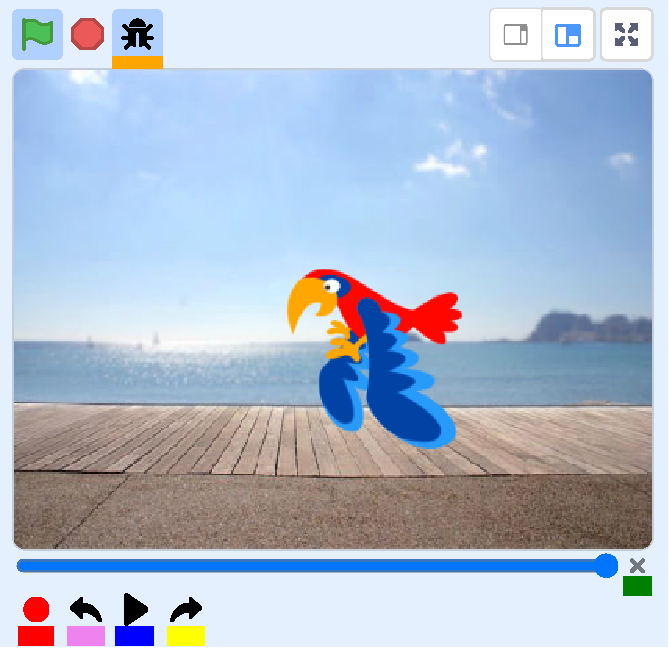
\includegraphics[width=\textwidth]{scratch-blink/ide}
    \caption{
        Blink additions to the controls and canvas of the Scratch environment.
        The bug-shaped button (underlined in orange) enables and disables the debugger.
        It is the only Blink addition that is visible in the environment in normal mode.
        Other additions become visible when in debug mode.
        The back-in-time slider underneath the canvas shows the progress of the recording and allows users to jump back and replay the recording.
        The small button to the right of the slider (underlined in green) allows the user to clear the recording.
        The red dot (underlined in red) indicates if recording is active by blinking.
        The back, play/pause, and forward buttons (underlined in pink, blue and yellow) allow the user to control either the recording or the execution.
    }
    \label{fig:blink-ide}
\end{figure}

The Blink debugger is built on top of and adds extra functionality to the Scratch environment (\cref{fig:blink-ide}).
When the debugger is disabled, all functionalities of the base Scratch environment remain unchanged.
To activate (and deactivate) debug mode, the user must press the bug-shaped button above the canvas.
While the debugger is active, the navigation bar turns green as a visual aid.
This way, a clear distinction is made between the default Scratch execution mode and debug mode.

\subsection{Stepwise execution}\label{subsec:stepwise-execution}
While the debugger is active, the execution of the Scratch project can be paused.
In this state, execution can be continued in a stepwise manner, with the step button.
Pressing this button will execute exactly one block in all scripts for which there is a corresponding thread in the \texttt{Runtime} (see \cref{subsec:instrumentation-for-stepping}).
After each step, the execution will pause again.
This way, the programmer can execute the program at their own pace, providing greater understanding of the impact of each block on the program state and making it easier to identify where errors may occur.
To return to the normal execution of the program, the resume button can be used (the same button as the pause button: which changes shape based on the execution state).

To be able to closely follow how a Scratch program is executed, Blink highlights blocks in the workspace with a dark grey hue.
During the execution of the program, these are the next blocks that will be executed in each active script.
These blocks are also highlighted when replaying a recording of the program.

\subsection{Back-in-time debugging}\label{subsec:back-in-time-debugging}
Finally, Blink allows replaying the last execution (i.e.\ the recording) of a Scratch program, inspired by back-in-time debuggers.
These debuggers allow the programmer to go back in the execution, often by recording program execution~\autocite{barrTardisAffordableTimetravel2014,barrTimetravelDebuggingJavaScript2016,czaplickiAsynchronousFunctionalReactive2013,balzerEXDAMSExtendableDebugging1969,ungarDebuggingExperienceImmediacy1997,chenReversibleDebuggingUsing2001,crescenziReversibleExecutionVisualization2000}.
When the debugger is active, a recording is automatically made, as can be seen on the slider below the canvas.
Selecting a point on the slider or pressing the back button will pause execution, and the selected point in the recording will be restored.
This includes the entire visual state of all sprites and their clones.
While back-in-time debugging is a quite complex debugger feature, our experimental study in \cref{subsec:blink-experimental-study} shows that providing a simple video-player-like interface is intuitive for young students.

\subsection{Programmed breakpoints}\label{subsec:programmed-breakpoints}

\begin{varwidth}{0.2\linewidth}
    \begin{scratch}[scale=0.6]
        \blockdebug{pause}
    \end{scratch}
\end{varwidth}%
\hspace{1em}%
\begin{varwidth}{0.4\linewidth}
    \begin{scratch}[scale=0.6]
        \blockdebug{pause if \emptybooldebug}
    \end{scratch}
\end{varwidth}%
\hspace{1em}%
\begin{varwidth}{0.5\linewidth}
    \begin{scratch}[scale=0.6]
        \blockdebug{wait until \emptybooldebug{} and pause}
    \end{scratch}
\end{varwidth}%

Blink adds three custom blocks to Scratch to manually program breakpoints.
Additionally, \setscratch{scale=0.5}\booldebug{debugger is enabled?} reports whether the debugger is currently active or not.
When in debug mode, the execution of the pause block suspends the Scratch program.
In contrast, the pause block represents a conditional breakpoint that only pauses the execution if its corresponding condition evaluates to true.
The wait until and pause block waits until a condition holds and then suspends the execution.

\section{Software architecture}\label{sec:blink-software-architecture}

Internally, Scratch consists of several interconnected components implemented in JavaScript (\cref{sec:scratch-internal}).
However, for the integration of Blink, changes were only made in the virtual machine and the user interface.
The interaction between these two components is shown in \cref{fig:blink-architecture}.

The Blink debugger consists of three main components: instrumentation of the virtual machine for stepping, recording of the execution state, and the custom debug extension, which implements the breakpoints.

\begin{figure}
    \centering
    \includestandalone[width=\linewidth]{scratch-blink/architecture}
    \caption{
        Sequence diagram showing the interactions in the virtual machine relevant to the debugger.
        From the user interface (grouped as ``External'' in the diagram), the \texttt{Runtime} receives events, in response to which threads are created or removed.
        Meanwhile, the \texttt{\_step} method is called 30 times per second (this is implemented inside the \texttt{Runtime}, but should be considered external).
        This method manages the threads, and calls \texttt{stepThreads}, which will then call \texttt{stepThread} for each thread in the virtual machine.
        This last method will finally call the \texttt{execute} method on the \texttt{Execute} class, which will do the actual executing.
    }
    \label{fig:blink-architecture}
\end{figure}

\subsection{Instrumentation for stepping}\label{subsec:instrumentation-for-stepping}

The virtual machine executes Scratch programs and preserves their current state.
It consists of three main modules: the \texttt{Runtime}, the \texttt{Sequencer}, and the \texttt{Execute} module.
The \texttt{Runtime} module maintains a list of active threads.
These objects embody the execution state of a script.
Threads are created when certain events trigger (i.e.\ a green flag is clicked), but can also be removed from the runtime (i.e.\ when deleting a clone).
A Scratch program is executed by repeatedly calling the \texttt{\_step} method of the \texttt{Runtime}, typically 30 times per second.
This method subsequently manages threads and calls \texttt{stepThreads} as shown in \cref{fig:blink-architecture}.
This will then call \texttt{stepThread} for each thread in the virtual machine.
This last method will finally call the \texttt{execute} method on the \texttt{Execute} class, which will do the actual executing.

Blink implements the pause, step, and resume commands of the debugger by instrumenting the \texttt{\_step} method of the \texttt{Runtime}.
The instrumentation consists of injecting the code for recording state into this \texttt{\_step} method in the Blink fork of the Scratch virtual machine.
If the execution of the program is paused, no steps will be taken.
It is important to note that all other tasks performed by the \texttt{\_step} method will still be carried out.
Therefore, user actions will continue to result in the creation of threads, which will, however, not be executed.

If, on the other hand, the execution is paused, but a step is taken, the \texttt{\_step} method will execute one block for each active thread.
If the execution is not paused, the \texttt{\_step} method behaves as normal.

The definition of a step in Blink differs from the \texttt{\_step} method in the virtual machine and does not execute a single block, as the step functionality does in a traditional debugger.
This is a consequence of the Scratch execution model, which presents a dichotomy between code execution and user observable state.
The former is inherently sequential: the virtual machine executes one block after the other, decides when a thread switch is needed, and in what order threads are executed.
The latter is inherently concurrent: multiple sprites/clones act at the same time.

In Blink, we prioritize maintaining the observed concurrency by ensuring that when stepping through the code, all scripts advance simultaneously for focused debugging.
This approach allows users to keep focus on relevant scripts without distractions from visible thread switches or manual stepping, which can be cumbersome in complex programs.
Users can thus focus on the script(s) they believe are involved in the failure while ignoring (correct) scripts running at the same time.
We discuss this more in great depth in \cref{ch:scratch-execution-model}.

\subsection{Back-in-time debugging}\label{subsec:arch-back-in-time-debugging}
Blink also offers back-in-time debugging capabilities.
During a debugging session, it instruments the virtual machine and constructs a snapshot of the program state each time a step is executed.
These snapshots contain the entire state of the Scratch program, including the position of the sprites, the active blocks, clones, and the pen.
To implement this feature, we modified the \texttt{Execute} component (\cref{fig:blink-architecture}) to create a snapshot at the end of the \texttt{execute} method.
Once a debugging session has been completed, these snapshots can be consulted to restore the program state.

\subsection{Programmed breakpoints}\label{subsec:arch-programmed-breakpoints}
Pausing the execution of a running program by manually stepping and pausing the execution can rapidly become tiresome.
Therefore, many debuggers include the ability to set user-defined breakpoints.
In Blink, we have extended the block language to include four additional blocks to pause the execution of a program, to inspect whether the debugger is active and to stop the program based on a condition.

In our original design, we experimented with a large set of highly specific debugging blocks, for example, a block to stop execution when a sprite hits the wall.
However, we came to the conclusion that it would be impossible to account for every possible use-case.
Therefore, we decided it would be better to provide a small set of fundamental debugging blocks, which can be composed with existing Scratch blocks to express more specific debugging blocks.

\section{Examples}\label{sec:blink-illustrative-examples}

In this section, we give two illustrative examples to demonstrate how Blink assists in detecting bugs in Scratch programs.
The first project consists of guiding a sprite through a maze without going through the walls.
The second project is a typical logo exercise where a sprite needs to walk over a star figure without falling into the surrounding water.
These projects are typical Scratch exercises where we believe the debugger can be helpful in finding bugs easier and faster.

\subsection{\emph{Maze} exercise}\label{subsec:maze-exercise}

\begin{figure}
    \begin{wide}
        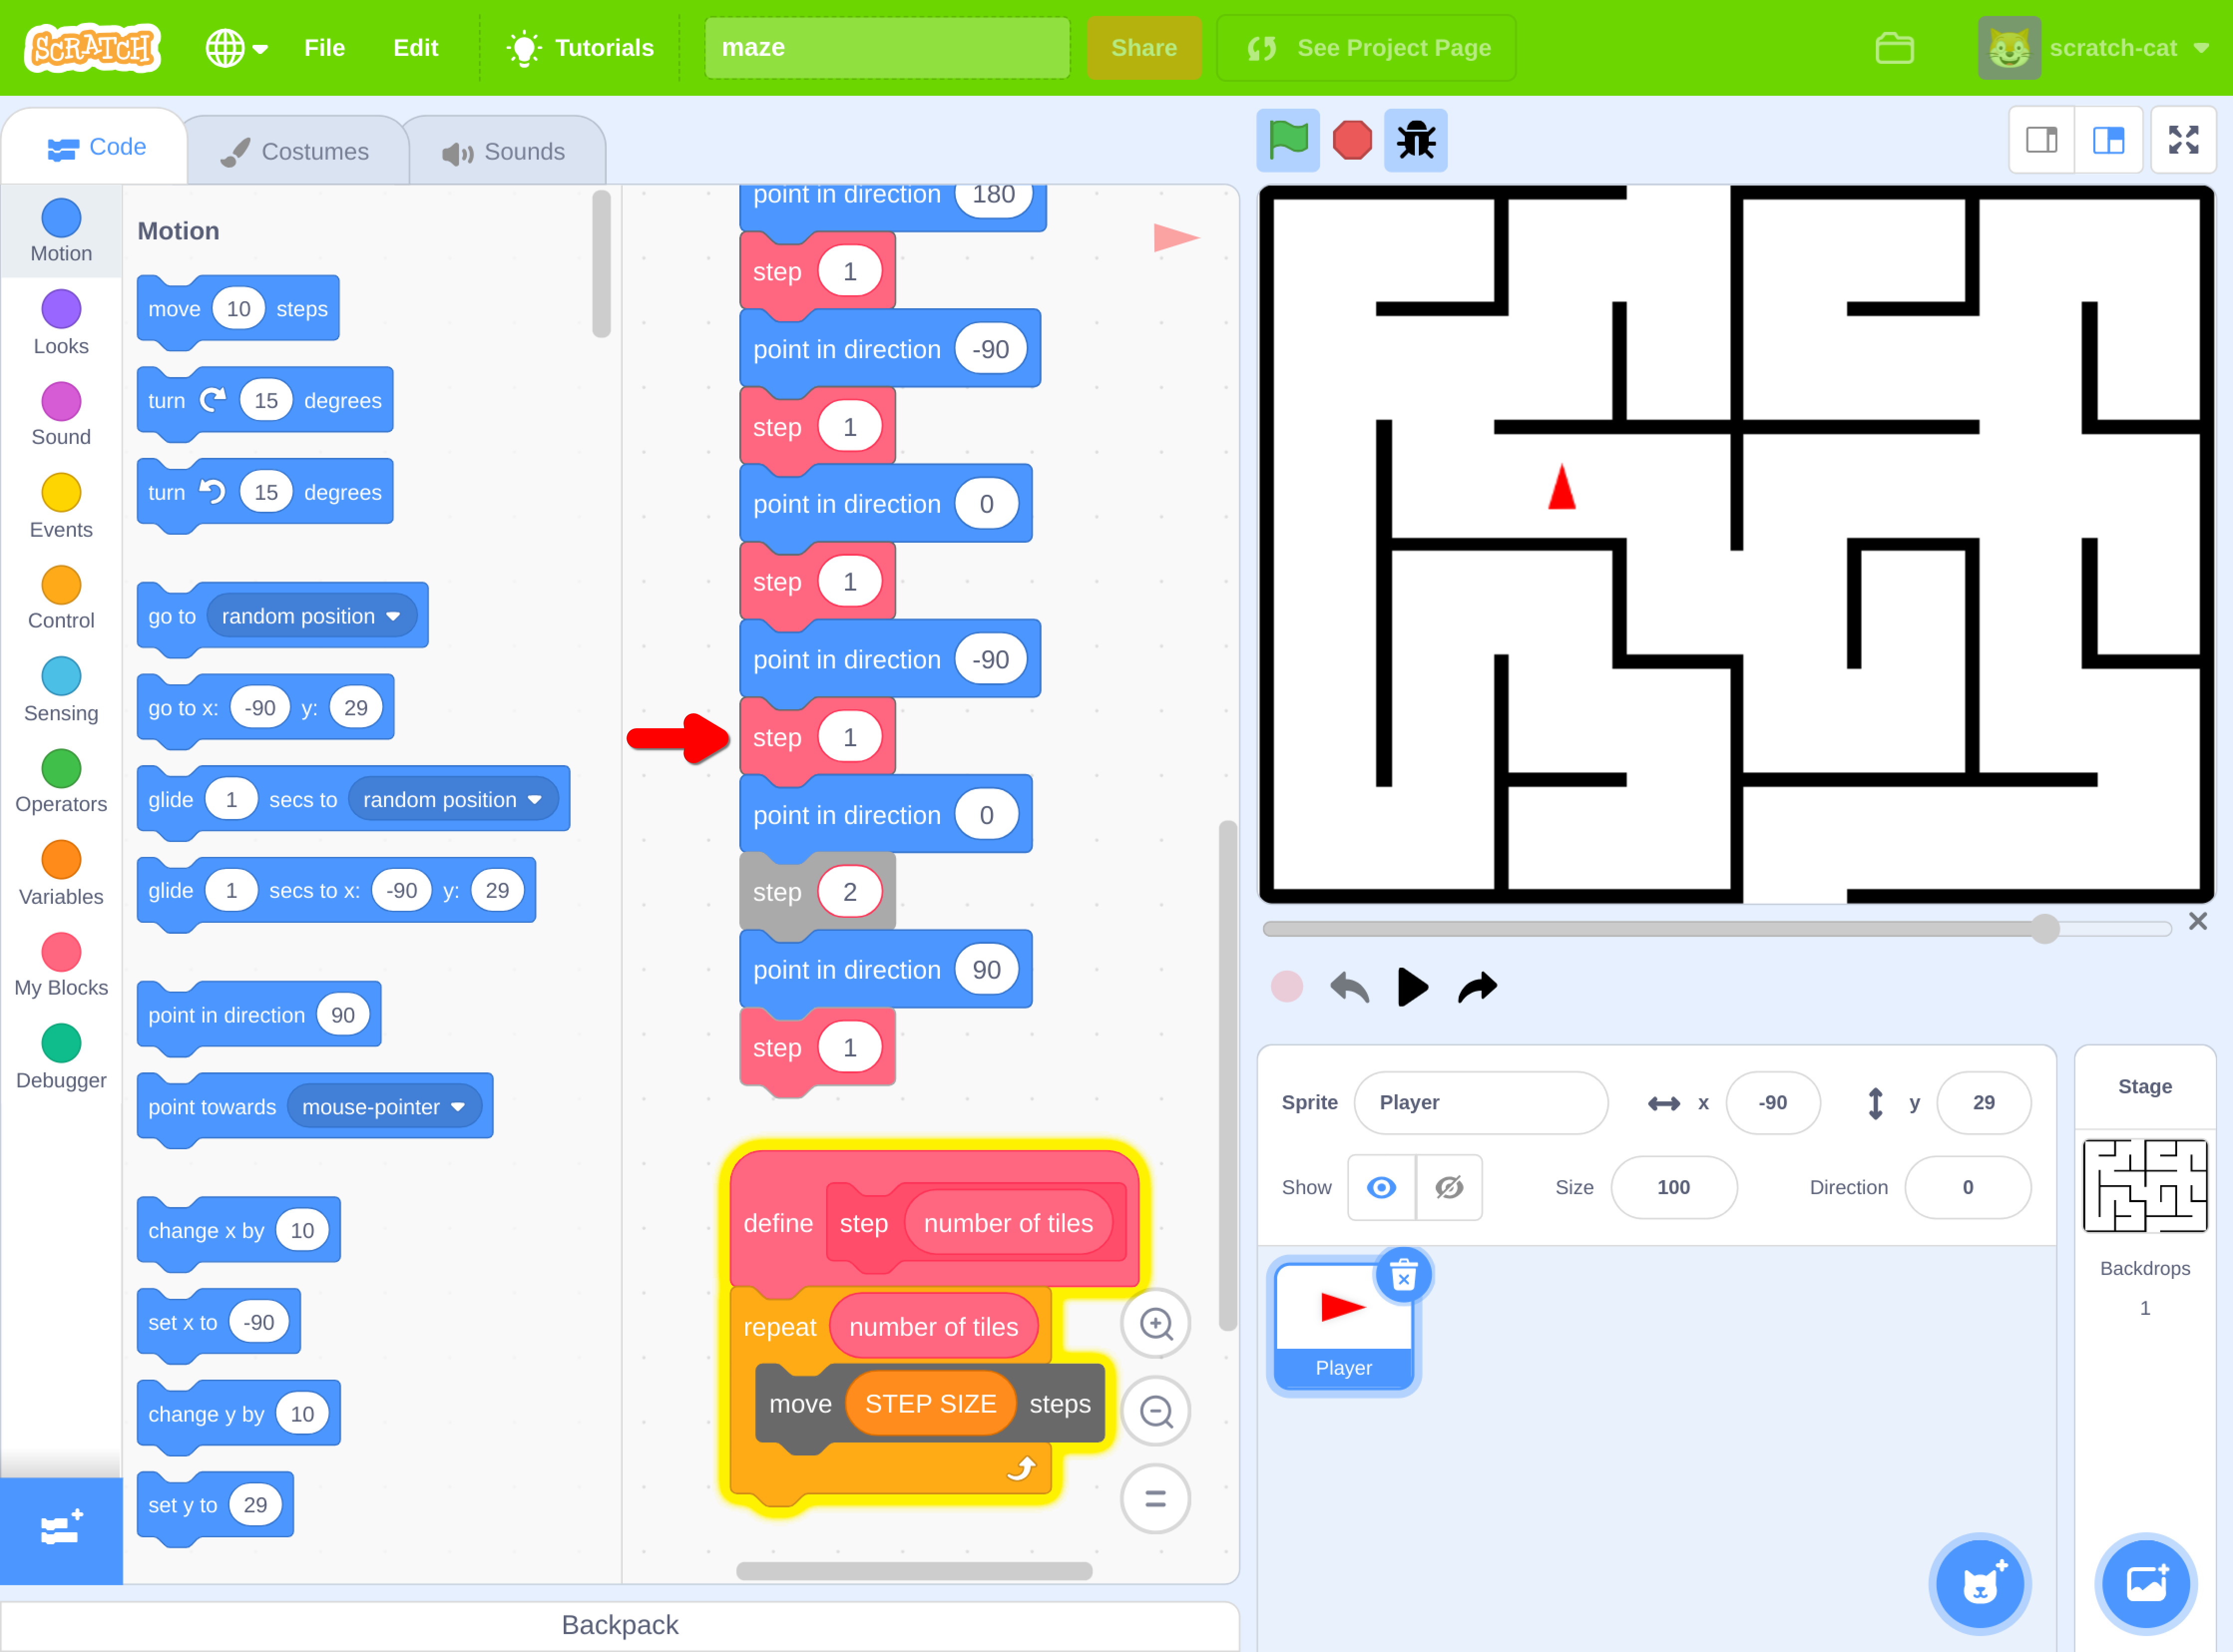
\includegraphics[width=\linewidth]{scratch-blink/maze}
    \end{wide}
    \caption[The Maze exercise.]{
        The \emph{Maze} exercise.
        The execution is paused before the failure occurs.
        As indicated by the light grey colour, we are in the \scratchinline{\blockmoreblocks{step \ovalnum{2}}} block.
        The next block is the \scratchinline{\blockmove{move \ovalvariable{STEP SIZE} steps}} block, as indicated in dark grey.
        However, since the sprite Player is pointing upwards, it will go through the wall.
        The bug is in the \scratchinline{\blockmoreblocks{step \ovalnum{1}}} block indicated by the red arrow.
        The solution is to replace this block with a \scratchinline{\blockmoreblocks{step \ovalnum{2}}} block: in which case the Player would have moved one square more to the left, meaning the Player can go up without going through a wall.
        Note that further changes are needed to reach the exit of the maze.
    }
    \label{fig:maze}
\end{figure}

The \emph{Maze} exercise involves a single sprite in the shape of a red triangle representing the player.\footnote{\url{https://scratch.ugent.be/blink/editor?project=/blink/maze.sb3}}
The goal of the exercise is to write a program that navigates the player through the maze when the user presses the green flag.
Correctly navigating consists of not letting the player navigate through the walls of the maze.
In \cref{fig:maze} we show code, which seems to navigate the player through the maze correctly when executing the project.
Unfortunately, there is a small mistake towards the end of the solution, which is difficult to see when executing the program at full speed.
By making use of the debugger, it becomes easy to navigate through the execution of the program step-by-step, which makes it apparent where the player has taken a misstep.
Additionally, due to back-in-time debugging, it is easy to trace back to precisely where the bug emerged in the code.
With more traditional debuggers, which only provide step-wise execution, programmers frequently discover program errors too late, necessitating restarting the complete debugging session.

\subsection{\emph{Star} exercise}\label{subsec:star-exercise}

\begin{figure}
    \begin{wide}
        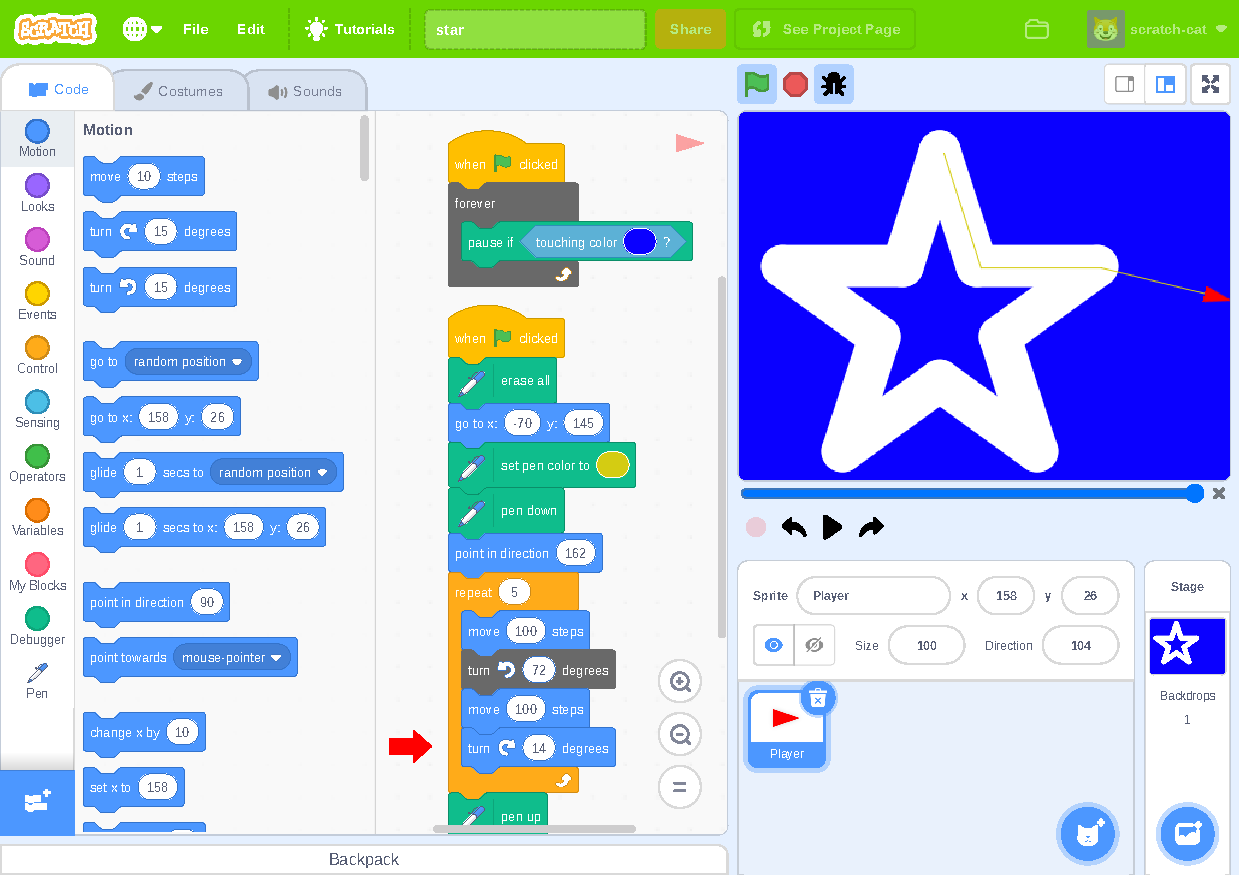
\includegraphics[width=\linewidth]{scratch-blink/star}
    \end{wide}
    \caption[The Star exercise.]{
        The \emph{Star} exercise, which has two scripts.
        The bottom script contains a bug: the \scratchinline{\blockmove{turn \turnright{} \ovalnum{14} degrees}} block (red arrow) should be a \scratchinline{\blockmove{turn \turnright{} \ovalnum{144} degrees}} block.
        The top script helps to find the bug: once running, the code loops forever, evaluating the breakpoint each time, and pausing execution if the condition is true.
    }
    \label{fig:star-exercise}
\end{figure}

While the \emph{Maze} exercise demonstrates the capabilities of Blink in regard to step-wise execution and back-in-time debugging, the \emph{Star} exercise demonstrates the helpfulness of our custom debugging blocks.\footnote{\url{https://scratch.ugent.be/blink/editor?project=/blink/star.sb3}}
The aim of this exercise is to walk over a star-shaped figure surrounded by water.
Any program that directs the player into the water is buggy.
By making use of Blink's custom debugging blocks, it is quite easy to pause the execution of the program when the player touches something blue (\cref{fig:star-exercise}).
As soon as the green flag is clicked, the code repeatedly checks whether the player is touching something blue.
If it does, program execution is paused by using the \scratchinline{\blockdebug{pause if \emptybooldebug}} block.

\section{Impact}\label{sec:blink-impact}

\subsection{Related work}\label{subsec:related-work}
While most textual programming languages have debuggers, the emphasis in this chapter is on block-based languages.
In this domain (excluding Scratch), the most notable debuggers are the Microsoft MakeCode Arcade~\autocite{ballMicrosoftMakeCodeEmbedded2019} debugger and the Blockly debugger~\autocite{savidisCompleteBlockLevelVisual2020}.
Both of these debuggers offer basic debugging facilities, such as breakpoints, step functionality, and variable watches.
Unfortunately, these debuggers are not applicable to the Scratch environment because both MakeCode Arcade and Blockly assume a sequential execution model, while the Scratch programming language is inherently concurrent.
The Snap\textit{!} block-based programming language~\autocite{monigSnapBuildYour2024} does support concurrency, but its debugger lacks back-in-time debugging functionality.
Next to block-based programming languages, we have taken inspiration from back-in-time debuggers~\autocite{barrTardisAffordableTimetravel2014,barrTimetravelDebuggingJavaScript2016}.

For Scratch, we are aware of three existing debuggers.
The first provides pause/resume/step functionality and breakpoints~\autocite{wangDevelopingResourcesDebugging2021}.
The second debugger is a browser extension that provides breakpoints and advanced logging~\autocite{ScratchAddons2023}.
The last, and most recent, debugger is NuzzleBug~\autocite{deinerNuzzleBugDebuggingBlockBased2024}.
It provides similar functionality to Blink, but makes some different choices in its implementation and user interface.
For example, the step functionality in NuzzleBug is a more traditional step, advancing one block at a time.

The need for tools to help find bugs in Scratch projects is also illustrated by the existence of other tools.
These include multiple linter-style tools like Hairball~\autocite{boeHairballLintinspiredStatic2013}, Dr.\ Scratch~\autocite{moreno-leonDrScratchWeb2015}, QualityHound~\autocite{techapalokulQualityHoundOnline2017} and LitterBox~\autocite{fraserLitterBoxLinterScratch2021}, or test frameworks such as Whisker~\autocite{stahlbauerTestingScratchPrograms2019} and \textsc{itch}~\autocite{johnsonITCHIndividualTesting2016}.

\subsection{Experimental study}\label{subsec:blink-experimental-study}
To validate the usefulness of the debugger in helping students understand their code better, we conducted a quasi-experimental study~\autocite{shadishExperimentalQuasiexperimentalDesigns2002}.
The test group consisted of 16 students aged 8 to 11, which is at the lower end of Scratch's target audience.

Our experiment started with a short introduction explaining the different features of Blink and how they can be used.
Subsequently, we provided the students with two projects as discussed in \cref{sec:blink-illustrative-examples}.
Both projects contained an error leading to unwanted behaviour during the execution of the program.
During each exercise, we encouraged the students to make use of the features of the debugger to correct the implementation.

Our study aimed to determine the ease of use and usefulness of Blink.
Participants were asked to rate both aspects for three different aspects of the debugger tool: traditional debugger operations, usage of breakpoints, and back-in-time debugger.
A five-point scale, represented as a row of smiley faces, was provided for each statement.
The results of this questionnaire are shown in \cref{fig:blink-results}.

\begin{figure}
        % https://observablehq.com/d/b50757d4920f2318
    \centering
    \includestandalone{scratch-blink/likert}
    \caption{
        Answers regarding the ease of use and the usefulness of the debugger in general,
        the breakpoints and the ability to go back in time to detect errors.
    }
    \label{fig:blink-results}
\end{figure}

The findings indicate unanimous agreement among participants that revisiting previous states is a straightforward and advantageous approach for identifying errors in Scratch code.
The custom breakpoints were less intuitive for most students and received a lower score on ease of use.
While breakpoints were conceptually clear to most students, when they were asked to implement a custom breakpoint to pause the execution, many of them struggled.
Finally, if we look at the score distributions for the debugger in general, we can see that they embody the combination of the distributions for the usage of the breakpoints and the ability to go back in time.

\section{Conclusions}\label{sec:blink-conclusions}
In this chapter we introduced Blink, a debugger for the Scratch programming language.
Blink offers stepwise execution, back-in-time debugging, and the ability to define custom breakpoints.
These features allow students to closely follow the execution of their programs and consequently make it easier to find errors.
To evaluate the effectiveness of our debugger, we conducted a quasi-experimental study.
The results of this study show that most aspects of the debugger are both useful and easy to use.
We observed a strong preference for back-in-time debugging and observed that custom breakpoints are less intuitive than back-in-time debugging.
In future work, we will focus on inventing novel user interface elements to further improve the ease of use for programming custom breakpoints for students.

\chapter{The Scratch execution model}\label{ch:scratch-execution-model}

\dictum[Maloney \& Resnick, \textit{The Scratch Programming Language and Environment}]{Concurrency is often considered an advanced programming technique. Yet our everyday world is highly concurrent, so Scratch users
are not surprised that a sprite can do several things at once.}

The programming language Scratch inherently supports parallel programming.
Each Scratch program (called a project) consists of a number of sprites with individual code (\cref{ch:scratch-the-programming-environment}).
Blocks that are attached together form scripts, and each sprite can have multiple scripts running concurrently as separate threads within the Scratch virtual machine.

The Scratch execution model combines a fixed-step time loop (30 frames per second) with an almost-cooperative threading model.
This means that threads are seldom interrupted, mostly relying on explicit yielding to other threads.
While this approach minimizes the occurrence of certain race conditions, some concurrency issues persist~\autocite{maloneyScratchProgrammingLanguage2010}.
For instance, the order in which sprites respond to broadcasts can be unpredictable.
Consequently, even without explicit concurrency controls, Scratch is a useful tool for teaching concurrency concepts~\autocite{fatourouTeachingConcurrentProgramming2018}.

However, the current execution model has some drawbacks.
The cooperative nature of the threading model can lead to unexpected behaviour when working with multiple sprites.
Additionally, the execution model complicates the use of debuggers within Scratch.
A traditional step function (which steps one block at a time) exposes execution states that are normally hidden.
Alternative step functions (see, for example, the one used by Blink in \cref{subsec:stepwise-execution}) diverge from the normal execution and are thus undesirable.

To address these issues, this chapter begins with an in-depth exploration of Scratch's current execution model.
This analysis is essential for understanding the subsequent section, where we explore the model's shortcomings in more detail.
We then propose some modifications to the execution model, which would solve the issues we have identified.
These modifications are finally evaluated to determine their impact on real-world Scratch projects in a preliminary benchmark.

\section{Elements of a Scratch program}\label{sec:elements-of-a-scratch-program}

\begin{listing}
    \centering
    \begin{sublisting}{0.45\textwidth}
        \centering
        \begin{scratch}[scale=0.7]
            \blockinit{when \greenflag{} clicked}
            \blockmove{move  \ovalnum{100} steps}
            \blockmove{turn \turnleft{} \ovalnum{90} degrees}
            \blockmove{move  \ovalnum{100} steps}
            \blockmove{turn \turnleft{} \ovalnum{90} degrees}
            \blockmove{move  \ovalnum{100} steps}
            \blockmove{turn \turnleft{} \ovalnum{90} degrees}
            \blockmove{move  \ovalnum{100} steps}
            \blockmove{turn \turnleft{} \ovalnum{90} degrees}
        \end{scratch}
    \end{sublisting}
    \begin{sublisting}{0.45\textwidth}
        \centering
        \begin{scratch}[scale=0.7]
            \blockinit{when \greenflag{} clicked}
            \blockrepeat{repeat \ovalnum{4}}{
                \blockmove{move  \ovalnum{100} steps}
                \blockmove{turn \turnleft{} \ovalnum{90} degrees}
            }
        \end{scratch}
    \end{sublisting}
    \caption{
        Two Scratch programs that seemingly exhibit the same behaviour: the sprite moves in a square of 100 steps, and finally stops at the same position as the start of the program.
    }
    \label{lst:scratch-two-programs}
\end{listing}

A Scratch program consists of zero or more sprites and a stage (see also \cref{ch:scratch-the-programming-environment}).
For every sprite at least one target is created (a target is what is drawn on the screen), while the stage has exactly one target.
All targets have their own local state: the variables and visual properties (e.g.\ position, size, bounding box, colour, direction).
Clones create more targets of the same sprite.
While clones have their own separate state, all targets based on the same sprite share the same code.
In the virtual machine, there is no substantial difference between how targets from different origins (sprites, stage, clones) are handled, so we can just consider targets for the remainder of this chapter.

Code-wise, the Scratch blocks are organized into categories (see \cref{subsec:using-the-environment-and-the-blocks}).
However, in this case, it is useful to look at their technical type, which corresponds to their shape.
In total, there are seven types of blocks:

\begin{enumerate}[noitemsep]
    \item Hat blocks \scratchinline{\blockinit{\hspace{1em}\dots\hspace*{1em}}}, which are placed at the start of a script (they are named hat blocks since they visually sit on top of a script).
    A script can only have one hat block.
    They function as event listeners, which trigger execution of the script if the event occurs.
    \item Stack blocks \scratchinline{\blockmove{\hspace{1em}\dots\hspace*{0.5cm}}}, representing program statements.
    These are the most common blocks.
    They are called stack blocks since they are stacked on top of each other.
    Stack blocks broadly fulfil the role of statements in Scratch.
    \item C blocks \scratchinline{\blockif{\hspace{1em}\dots\hspace*{1em}}{\blockspace[0.2]}}, which are named after their shape.
    They are used for most of the control flow blocks: loops and branches.
    The variant for the if/else block is sometimes called an E block since it has two slots.
    \item Reporter blocks \setscratch{baseline=c,scale=0.5}\ovalmove{\hspace{1em}\dots\hspace*{1em}}, act as variables or values and can be slotted into other blocks.
    Operators that result in a value also have this shape.
    The reporter blocks fulfil the role of expressions.
    \item Boolean blocks \setscratch{baseline=c,scale=0.5}\boolsensing{\hspace{1em}\dots\hspace*{1em}}, which are analogous to reporter blocks but result in a boolean.
    \item Cap blocks \scratchinline{\blockstop{\hspace{1em}\dots\hspace*{1em}}}, which end a script: no blocks can be added afterwards.
    Note that the infinite loop block, for example, is both a C block and a cap block.
    \item Custom blocks \scratchinline{\initmoreblocks{define\hspace{1em}\dots\hspace*{1em}}}, which define ``procedures''.
\end{enumerate}

\section{Related work}\label{sec:execution-related-work}

The Scratch execution model is defined by its implementation in the virtual machine.
There exists, at least to the knowledge of the authors, no comprehensive formal description of the execution model.
This does not mean there is no prior work.
From the Scratch team, \textcite{maloneyScratchProgrammingLanguage2010} provide a high-level description of the threading model.

Another body of works that provides insights into the Scratch execution model comes from the \emph{Chair of Software Engineering II} group, led by Gordon Fraser.
These publications all provide descriptions for parts of the execution model.

First, \textcite{stahlbauerTestingScratchPrograms2019} propose a formalization of three aspects in Scratch: the user perspective, a syntactic model and a semantic model.
They describe the semantics of Scratch with a memory model based on message passing.
Next, \textcite{stahlbauerVerifiedScratchProgram2020} develop LeILa, an intermediate language to which Scratch projects can be translated, with the intended use of performing analysis on Scratch projects.
The authors also provide a formalization of LeILa, using approximations for the behaviour of Scratch in some areas.
Also, \textcite{gotzModelbasedTestingScratch2022} model the state-based behaviour of Scratch programs using a finite state machine.
Finally, \textcite{deinerAutomatedTestGeneration2023} delve deeper into the actual execution of the virtual machine, while also proposing some modifications to it, for example, to make execution deterministic.

Other block-based languages also have to deal with concurrency.
For example, MakeCode also uses a non-preemptive threading model, inspired by Scratch~\autocite{ballMicrosoftMakeCodeEmbedded2019}.
There has also been some work on concurrency and concurrency controls in other block-based languages~\autocite{chungConCodeItComparisonConcurrency2020}.
However, since these languages do not use the Scratch virtual machine for execution, their relevancy for this chapter is limited.

\section{The current execution model}\label{sec:the-current-execution-model}

\subsection{Execution of a Scratch program}\label{subsec:execution-of-a-scratch-program}

\marginnote{Arguably, it is more of a concrete syntax tree, as e.g. the position of blocks is also saved. However, in Scratch's case, the differences are minimal, so we call it an abstract syntax tree, as Scratch themselves do.}
When executing Scratch code, the virtual machine transforms the blocks into an abstract syntax tree.
These are organized by target, and every execution of a script results in a distinct thread inside the virtual machine.
These are green threads: implemented fully in the virtual machine.

The virtual machine is thus responsible for scheduling these threads.
\Cref{fig:blink-architecture} gives a schematic overview of the interaction between the different parts.
It uses an almost-cooperative threading model, which \textcite{maloneyScratchProgrammingLanguage2010} call the ``Scratch threading model''.
This means it is mostly non-preemptive: the virtual machine will not interrupt threads at arbitrary points in their execution.
The threads must voluntarily yield control or reach a limited set of points in their execution.
The rational is given in~\cite{maloneyScratchProgrammingLanguage2010}: ``Scratch builds concurrency control into its threading model in a way that avoids most race conditions, so that users do not need to think about these issues.
This is done by constraining where thread switches can occur.''.

At four well-defined points, a thread always yields, thus causing said thread switching:
\begin{enumerate}
    \item When a block with a fixed duration is executed.
    There are a number of blocks that fall under this category.
    \scratchinline{\blockcontrol{wait \ovalnum{}}} is an obvious inclusion, but this also applies to \scratchinline{\blockmove{glide \ovalnum{} secs to x: \ovalnum{} y: \ovalnum{}}}, for example.
    \scratchinline{\blocksound{play sound \ovalsound*{} until done}} also falls under this category, even if there is no explicit time.
    \item When a block waits on execution of other blocks.
    For example, \scratchinline{\blockevent{broadcast \selectmenu{something} and wait}}.
    \item The last block of a loop (thus \scratchinline{\blockinfloop{forever}{\blockspace[0.2]}}, \scratchinline{\blockrepeat{repeat \ovalnum{}}{\blockspace[0.2]}}, and \scratchinline{\blockrepeat{repeat until \boolempty[1em]{}}{\blockspace[0.2]}}).
    This means thread switching will occur after every loop iteration.
    \item A recursive procedure call is detected.
    Scratch attempts to detect these (up to five levels of indirection) and will yield the thread on each call if it detects a recursive call.
\end{enumerate}

There is one exception: when using procedures ``without screen refresh'', Scratch will interrupt a thread that runs longer than \qty{500}{\milli\second}.
This is called the ``wrap timer'', and has some curious edge cases.\footnote{\url{https://github.com/scratchfoundation/scratch-vm/issues/2834}}

The threads are executed in a first-come, first-serve manner: there are no priorities nor changes in thread order.
The first thread is executed until it yields or ends, then the next thread, and so on.
We call the execution within one thread until it yields or ends a \term{turn}.
A thread can have one of three conceptual states: \emph{done}, \emph{running}, and \emph{yield}.

\begin{figure}
    \centering
    \includestandalone{scratch-execution-model/scratch-model}
    \caption{Overview of the interplay between the threading model and the ``game loop''. Within one step (which is done 30 times per second), one or more ticks are executed. The arrow with \CircledText{2} illustrates this: after the first tick, another is started if less than \qty{75}{\percent} of the step time (the time one step has to complete, \qty{33}{\milli\second}) has been used, and a redraw has not been requested, and Scratch is not in turbo mode. Within one tick, a turn is executed for each thread \CircledText{1}: a thread executes until it terminates or the thread yields.}
    \label{fig:scratch-model-explained}
\end{figure}

\marginnote{Scratch 3 should actually run at \qty{60}{\fps}; however Scratch enables a compatibility mode by default, resulting in \qty{30}{\fps}.}
The virtual machine uses a \emph{fixed-time step with synchronization} main loop~\autocite{nystromGameProgrammingPatterns2014}, also called a \emph{synchronized coupled model}~\autocite{valenteRealTimeGame2005}.
This means that the virtual machine runs in \term{steps}: internally, the \texttt{step} function is called every \qty{33}{\milli\second} (so 30 times a second, commonly known as \qty{30}{\fps}).

In each step, the virtual machine will execute one or more ticks.
A \term{tick} is one turn in every thread: the first thread is executed until it yields or terminates, then the second thread and so on.
After the tick, a redraw is performed if needed (in practice this is always done, as the source code contains a to-do to implement selective redrawing).
After the first tick is finished, the virtual machine decides whether to run another tick (\cref{fig:scratch-model-explained}).
A new tick is started if less than \qty{75}{\percent} of the step time (the time one step has to complete, \qty{33}{\milli\second}) has been used and a redraw has not been requested.
Note that once a tick has started, it is run completely and cannot be stopped.
The arbitrary \qty{75}{\percent} is intended to prevent frame drops: steps that take longer than their allocated step time, meaning the next step is delayed.
Also, in practice, many blocks request a redraw, so in many Scratch projects, a step only ever runs one tick.

\begin{figure}
    \centering
    \begin{subfigure}{0.40\textwidth}
        \includestandalone{scratch-execution-model/threading-no-loop}
    \end{subfigure}
    \begin{subfigure}{0.59\textwidth}
        \includestandalone{scratch-execution-model/threading-with-loop}
    \end{subfigure}
    \caption{The execution of the two programs from \cref{lst:scratch-two-programs}. In the unrolled version (left), all code is executed in the first turn, meaning only one tick and step is needed. In the version with loop (right), the loop yields after each iteration, meaning the rest of the step is filled with idle time. In total, four steps are needed. }
    \label{fig:scratch-two-execution}
\end{figure}

A concrete example of the execution model is given by \cref{fig:scratch-two-execution}, which shows the execution of the programs from \cref{lst:scratch-two-programs}.
These programs have only one thread.
Since none of the blocks in the unrolled program yield the thread, the full program is executed in one tick.
In the other version, with a loop, the thread yields after each iteration of the loop, meaning the program needs four steps.
This does result in an observable difference: in the unrolled program, the sprite does not move visually.
As a redraw only happens between steps, the sprite is back at its original position.
In the looped version, the sprite moves four times (albeit rapidly), as there is a redraw between each step.

\subsection{Implementation details}\label{subsec:implementation-details}

How different parts of the virtual machine implement the execution model from \cref{subsec:execution-of-a-scratch-program} is shown in \cref{fig:blink-architecture}.
When the user interface loads a project, it also starts the virtual machine.
This means that the game loop is active (this is done in the class \texttt{Runtime}).

New threads are only created in two scenarios:
\begin{itemize}[noitemsep]
    \item Code needs to be executed, either because an event triggered some hat blocks (green flag, key press, etc.) or because the user clicked on some blocks.
    \item When ``stage monitors'' or watchers are active.
    These are used in the user interface to show the value of variables or properties.
    The watchers for variables also allow the user to change the value of the variable.
\end{itemize}

The \texttt{Runtime} calls the method \mintinline{javascript}{stepThreads} in the \texttt{Sequencer} class.
This class is responsible for implementing the ticks.
After each tick, done threads are removed, and a new tick is started if possible.
It is also here that the thread status is managed.
While there are three conceptual statuses, the implementation has five:
\begin{description}[noitemsep]
    \item[\texttt{done}] The thread has finished executing all blocks and will be removed after this tick.
    \item[\texttt{running}] The thread is being executed and has more blocks to execute.
    It will be scheduled again next tick.
    \item[\texttt{yield}] The thread is waiting an amount of time.
    The thread is scheduled again next tick to see if the wait time is over.
    \item[\texttt{promise wait}] The thread is waiting for a JavaScript promise to be resolved, after which the thread will be set to \texttt{running}.
    \item[\texttt{yield tick}] The thread yields until the next step.
    The purpose of this status seems to be some performance optimizations to aid with benchmarking.\footnote{\url{https://github.com/scratchfoundation/scratch-vm/pull/1211}}
\end{description}

Each thread maintains a stack structure.
The \texttt{Sequencer} will then look up the next block on said stack, and if there is one, it will call the \texttt{Execute} class.
That class will actually execute the block on the stack.
For normal blocks (somewhat confusingly called ``stack blocks'', since they stack together to form a script), the current block is popped from the stack, the block is executed, and the next block is put on the stack.
The stack is only useful when working with C-blocks or procedures.
For example, C blocks will push the first block in their slot on the stack.
In the case of a loop, a counter is saved in the stack frame to determine how many times the loop should be run.
The exact implementation of the stack is less relevant for this chapter, so it is left to the reader to browser the source code.

\section{Limitations of the execution model}\label{sec:limitations-of-the-execution-model-for-the-debugger}

This section illustrates a few limitations of the current execution model, first in general and then specifically for a debugger.

\subsection{During general execution}\label{subsec:in-general}

\begin{listing}
    \centering
    \begin{scratch}[scale=0.6]
        \blockinit{when \greenflag{} clicked}
        \blockmove{go to x: \ovalnum{0} y: \ovalnum{112}}
        \blockpen{erase all}
        \blockpen{set pen color to \pencolor{ppcolor}}
        \blockpen{set pen size to \ovalnum{5}}
        \blockpen{pen down}
        \blockmove{point in direction \ovalnum{108}}
        \blockrepeat{repeat \ovalnum{4}}{
            \blockmove{move \ovalnum{80} steps}
            \blockmove{turn \turnright{} \ovalnum{36} degrees}
            \blockmove{move \ovalnum{80} steps}
            \blockmove{turn \turnright{} \ovalnum{36} degrees}
        }
        \blockpen{pen up}
    \end{scratch}
    \hspace{3em}
    \begin{scratch}[scale=0.6]
        \blockinit{when \greenflag{} clicked}
        \blockinfloop{forever}{
            \blockif{if \boolsensing{touching color \pencolor{blue}} then}{
                \blockstop{stop \selectmenu{all}}
            }
        }
    \end{scratch}
    \caption{The implementation, with a bug in the first script (left) and a non-working second script (right).}
    \label{lst:star-model-implementation}
\end{listing}

\begin{figure}
    \begin{subfigure}{0.45\textwidth}
        
\includegraphics[width=\textwidth]{scratch-execution-model/star-before}
        \caption{The stage before execution.}
        \label{fig:star-exercise-model-before}
    \end{subfigure}
    \hfill
    \begin{subfigure}{0.45\textwidth}
        
\includegraphics[width=\textwidth]{scratch-execution-model/star-after}
        \caption{The stage after execution.}
        \label{fig:star-exercise-model-after}
    \end{subfigure}
    \caption{Result of running the implementation from \cref{lst:star-model-implementation} for the \emph{Star} exercise.}
    \label{fig:star-exercise-model}
\end{figure}

As \textcite{maloneyScratchProgrammingLanguage2010} mentioned, the Scratch threading model does not solve all issues with concurrency.
To illustrate this point, we will consider a variant on the \emph{Star} exercise from \cref{subsec:star-exercise}.
In this exercise, the goal is to let a sprite move around on a path without falling into the water (read: touching a blue colour).
\Cref{lst:star-model-implementation} shows an implementation for this exercise with an additional script that will stop execution if the sprite touches something blue.
We asked a number of educators that had experience with Scratch to predict the behaviour of this implementation.
All of them expected the execution to stop either when the sprite first touches the water or after executing the block when the sprite first touches the water.
However, as can be seen in \cref{fig:star-exercise-model}, where the canvas is shown before and after running the code, the second script that should have stopped execution did not work.

The reason for this is the non-preemptive thread switching: the body of the loop is always executed atomically.
At the start of the loop, the sprite does not touch the water.
After execution of one iteration, the sprite is back on the path and does not touch the water.
Therefore, whenever the second script is executed, the sprite is not touching the water, which explains why the execution was not stopped.

Consider the original code in the \emph{Star} exercise from \cref{subsec:star-exercise}.
The second script there does not stop the execution, but uses Blink's pause block to halt the execution.
Using the current execution model, the pause block will not function for the same reasons mentioned above.

\subsection{Specifically for a debugger}\label{subsec:specifically-for-a-debugger}

A fundamental feature of any debugger is the ability to step through code: executing one statement and then pausing the execution to facilitate inspection of the program state.
The functionality is also essential in debuggers for Scratch: all existing debuggers for Scratch implement it.
In Scratch, executing a single statement translates to executing a single block.

However, traditional single-block stepping has some drawbacks in Scratch.
A first drawback is that users have to click a lot, since the stepping functionality is global, not per thread.
Secondly, and more importantly, the step functionality exposes details of the Scratch execution model to the users.
For example, thread switching, which is normally implicit in Scratch's perceived parallel execution, becomes visible to the users during debugging.

Additionally, debuggers must choose what to do with intermediate states that are typically hidden during normal execution.
For instance, five consecutive blocks would result in one redraw in the normal execution.
One choice is to not alter the redraw logic (thus only redrawing when the normal execution would redraw), but this results in steps having no visual impact, even if the block logically should change the visuals.
The other choice is to redraw after every step.
While the effect of every block (and step) is then visible, this exposes intermediary steps that would normally not be drawn.
Some blocks (for example, checking if a sprite touches a colour) use the visual state, meaning these additional redraws can result in a different execution of the project.

As described in \cref{sec:blink-software-architecture}, our debugger Blink takes a different approach to the stepping feature.
We believe it is useful to maintain the observed parallelism of Scratch in the debugger: we define a step in the debugger as executing one block in every thread.
This approach allows users to keep focus on relevant threads without distractions from thread switches, which can be cumbersome in complex programs.
Users can thus focus on the script(s) they believe are involved in the failure while ignoring (correct) scripts running at the same time.

This approach does come at a price: it changes the Scratch execution model, which is not trivial due to two main considerations:

\begin{enumerate}
    \item If the execution model is only changed when debugging, the debugger does not debug the same program execution as when running the program.
    This can result in different behaviour, meaning the bugs for which the debugger is used need no longer be present or new bugs, unique to the debugger, could be introduced.
    \item If the execution model is changed, we need to ensure that existing Scratch programs keep working and that we do not introduce concurrency problems, as the current execution model of Scratch was explicitly chosen to avoid those.
\end{enumerate}

We opt for the second option: modifying the Scratch execution model.
In the next section, we discuss what we changed, after which we investigate the impact on performance and behaviour of existing Scratch projects.

\section{Towards a new execution model}\label{sec:a-family-of-new-execution-models}

In line with how we want the stepping feature of the debugger to work, we have decided to change the Scratch execution model as follows: we modify a turn to execute exactly one block before yielding.
Thus, in a single tick, the virtual machine will execute a single block in every thread.

As there is often only one tick per step (due to many blocks requesting redraws), this means that only one block would be executed per step (thus one block for every thread per \qty{33}{\milli\second}).
Consequently, this makes execution slower than in the original execution model.

A possible remedy is to modify the number of steps that are taken.
For example, it might be better to run at twice or more times the number of steps per second.
In turbo mode, this would mean the steps are done as fast as the hardware allows.
While this does make everything go much faster, it does introduce a big difference in execution time between a performant machine and a slower machine.

These changes to the execution model have as a benefit that the \emph{Star} solution (\cref{lst:star-model-implementation}) will behave as expected, since the first thread will yield after the first block in the loop.
It can also illustrate that this does introduce concurrency considerations that were not present in the original execution model.
For example, if the conditional block in the second thread evaluates to true, the first thread will execute another block before execution is stopped by the block inside the conditional block from thread two.

In the next section, we analyse existing Scratch projects to determine which frame rate for the new execution model most closely results in the same execution speed as the original execution model (which runs at 30 frames per second).
We also take this opportunity to analyse the complexity and block use in Scratch projects, to evaluate whether the concurrency considerations would cause problems.

\section{Exploration of Scratch projects}\label{sec:evaluation-of-scratch-projects}

As Scratch is used by many people, it is important that changes to the execution model do not adversely affect existing Scratch projects.
However, this requires us knowing what Scratch projects look like.
The aim of this analysis is to determine what blocks are used in Scratch projects, how big projects are, and what programming concepts are used.

We begin by looking at existing work on analysing Scratch projects, followed by our own analysis.

\subsection{Existing analyses}\label{subsec:existing-analyses}

\makenote*{There is some discussion if the cyclomatic complexity is a useful metric. It might have no more predictive ability than lines of code \autocite{hattonInvitedTalkRole2008,fentonCritiqueSoftwareDefect1999,cherfInvestigationMaintenanceSupport1992}.\vspace{0.5cm}}
\Textcite{aivaloglouHowKidsCode2016} analysed \num{250000} Scratch 2.0 projects they scraped from the public Scratch site.
They looked at the types of blocks used, the size of the projects, and the complexity.
For the complexity, they utilize the cyclomatic complexity metric~\autocite{mccabeComplexityMeasure1976}.
The considered decision points are the \texttt{if} and \texttt{if-else} blocks.

They found that most Scratch projects are small: \qty{75}{\percent} have less than 5 sprites, 12 scripts, and 76 blocks.
\qty{25}{\percent} has less than 12 blocks, although there are some huge projects with more than \num{20000} blocks.
They also found that about \qty{78}{\percent} of projects have no decision points.

\Textcite{fronzaApproachEvaluateComplexity2020} investigate Scratch projects with different complexity metrics.
The dataset is, however, much more limited: 80 projects were analysed.
\makenote*{The usefulness of the Halstead metrics is even more controversial~\autocite{hamerHalsteadSoftwareScience1982,shenSoftwareScienceRevisited1983,jonesDimensionalAnalysisHalstead2019}.}
The authors also measure the cyclomatic complexity, in addition to some Halstead complexity measures~\autocite{halsteadElementsSoftwareScience1977}, and their own proposal for a ``when'' metric.
They do use more decision points for the cyclomatic complexity (\texttt{if}, \texttt{if-else}, \texttt{repeat until}, \texttt{wait until}, \texttt{and}, \texttt{or}).
The proposed ``when'' metric counts the number of ``when'' blocks (e.g.\ hat blocks with certain conditions).

\subsection{A new dataset of Scratch 3.0 projects}\label{subsec:a-new-dataset-of-scratch-projects}

Since the dataset used by \textcite{aivaloglouHowKidsCode2016} consists of Scratch 2.0 projects and \textcite{fronzaApproachEvaluateComplexity2020} only analyse 80 projects, we found it necessary to collect a new dataset of Scratch projects.

We constructed a new dataset as follows, using the Scratch website.\footnote{\url{https://en.scratch-wiki.info/wiki/Scratch_API}}
Creating a new project provides an identifier ({\addfontfeature{Numbers={Lining,Proportional}}996725074}, April 7th, 2024), which we used as a starting point.
We then subtract one from the identifier, downloaded the project if possible, and continued.
\marginnote{The \num{1129465} projects were created in approximately 3 days, illustrating Scratch's popularity.}
The oldest project in the dataset is from April 5th, 2024, with identifier {\addfontfeature{Numbers={Lining,Proportional}}995595608}.

This resulted in \num{237926} downloaded public projects (of the total \num{1129465} that were made between our newest and oldest projects).
From those, \num{207} were corrupt or for an older version of Scratch.
We also filtered out the following projects: \num{37936} (\qty{15.9}{\percent}) were empty and \num{4411} (\qty{1.9}{\percent}) had no executable code (e.g.\ only head blocks or scripts without head blocks).
This results in a final dataset of \num{195372} Scratch projects we considered for further analysis.

\subsection{Analysing Scratch 3.0 projects}\label{subsec:analysing-scratch-3.0-projects}

Hairball~\autocite{boeHairballLintinspiredStatic2013} was commonly used to analyse Scratch projects (it is also used by the existing analyses), but does not support Scratch 3.0.
For this reason, we have implemented a similar tool in JavaScript (versus Hairball's use of Python).\footnote{\url{https://github.com/scratch-ed/scratch-analysis}}
It also supports plugins to support extensions for other analyses.
Being written in JavaScript, it has the advantage that it can reuse parts of the Scratch virtual machine, like reading and parsing Scratch projects.

Wherever possible, we have used the same definitions and metrics as used by \textcite{aivaloglouHowKidsCode2016}, for ease of comparison.
Whenever a direct comparison is possible and relevant, we have included their data in \textit{italics}.
For example, \qty{75}{\percent} (\textit{\qty{60}{\percent}}) indicates our data shows \qty{75}{\percent}, while \citeauthor{aivaloglouHowKidsCode2016} found \qty{60}{\percent}.

\subsection{Use of blocks}\label{subsec:use-of-blocks}

Scratch blocks can be categorized into seven types, based on their shape (\cref{sec:elements-of-a-scratch-program}), their usage shown in \cref{fig:block-shapes}.
Blocks can also be put into categories (\cref{subsec:using-the-environment-and-the-blocks}).
The number of projects that use a block from a certain category is shown in \cref{fig:block-categories}.
Note that these numbers do not fully compare with \textcite{aivaloglouHowKidsCode2016}: since then, some new Scratch extensions were added, and the pen-related blocks have moved to an extension.

It is notable that extensions are not widely used: only \qty{12.2}{\percent} of projects use any extension.
The Pen extension is the most popular one, appearing in \qty{6.9}{\percent} of the projects.

\begin{figure}
    \centering
    \includestandalone{scratch-execution-model/block-shapes}
    \caption{
        Number of blocks by shape in all projects.
        The total number of blocks is \num{47808628}.
        Note that the \textit{forever} block is counted twice (as a cap block and a C block), and procedure-defining blocks are counted as hat blocks.
    }
    \label{fig:block-shapes}
\end{figure}

\begin{figure}
    \centering
    \includestandalone{scratch-execution-model/block-categories}
    \caption{
        Number of projects that use blocks from a certain category.
        Custom blocks are excluded, and all blocks for extensions are counted together.
        Bar colours correspond to the block category colours in the traditional Scratch 3.0 colour scheme.
    }
    \label{fig:block-categories}
\end{figure}

\subsection{Size and complexity}\label{subsec:size-and-complexity}

\begin{table}
    \centering
    \caption{
        Size and complexity statistics about the \num{195372} non-empty Scratch projects in our dataset.
        Unless otherwise noted, all numbers are shown per project and blocks are counted as logical lines of code.
        The first column of numbers reports the mean from \textcite{aivaloglouHowKidsCode2016} if available.
        The subsequent numbers are, in order, the mean and the five-number summary: the minimum, the first quartile, the second quartile (the median), the third quartile, and the maximum.
    }
    \label{tab:loc-scratch}
    \begin{wide}
        \addfontfeatures{Numbers={Monospaced,Lining}}
        \begin{tabular}{|l|S S|S[table-format=2.0]|S[table-format=2.0]|S[table-format=2.0]|S[table-format=2.0]|S[table-format=5.0]|}
            \hline
            {} & {\AtNextCite{\defcounter{maxnames}{1}}\citeauthor{aivaloglouHowKidsCode2016}} & {mean} & {min} & {Q\textsubscript{1}} & {Q\textsubscript{2}} & {Q\textsubscript{3}} & {max} \\
            \hline
            sprites (with code) & 5.68 & 4.98 & 1 & 1 & 2 & 5 & 1000 \\
            scripts (with code) & 17.35 & 19.73 & 1 & 2 & 4 & 11 & 9134 \\
            \hline
            blocks (logical lines) & 154.55 & 203.14 & 2 & 9 & 22 & 75 & 24084 \\
            blocks (physical lines) & {\textsc{n/a}} & 150.81 & 2 & 8 & 20 & 65 & 20249 \\
            dead blocks & {\textsc{n/a}} & 42.25 & 0 & 0 & 0 & 3 & 14912 \\
            \hline
            blocks per script & {\textsc{n/a}} & 10.30 & 1 & 2 & 5 & 10 & 5497 \\
            \hline
            \shortstack[l]{cyclomatic complexity \\ per script} & 1.58 & 1.85 & 1 & 1 & 1 & 2 & 5497 \\
            \hline
        \end{tabular}
    \end{wide}
\end{table}

\Cref{tab:loc-scratch} shows a summary of the project size for our dataset.
In the rest of this subsection, we detail some choices we made in analysing the projects and draw some conclusions.

When considering the size of a program, a frequently used metric is lines of code.
However, there is no universal agreed-upon manner in which to count lines of code~\autocite{nguyenSLOCCountingStandard2007}.
Two variants are frequently used: physical lines of code (the number of lines in the source files) and logical lines of code (an approximation of the number of statements or expressions).
While normally counting the physical lines of code is easy and counting logical lines requires some consideration, the reverse is true in Scratch.
To count logical lines of code, we can simply count all blocks.
For physical lines of code, we chose to count the number of ``main'' blocks in a script.
This means we do not count blocks used as arguments, e.g.\ the condition block of a loop is not counted.

When counting the number of scripts per project, we excluded scripts that consist only of a hat block, as these do nothing.
We similarly excluded sprites without code from the count of sprites per project.
These can have a role in some cases but are not useful in the statistics.

From these data, we can see that \qty{75}{\percent} of projects have less than 5 sprites, 11 scripts, and 80 blocks (\textit{\qty{75}{\percent} of projects have less than 5 sprites, 12 scripts, and 76 blocks}).
We can conclude that most Scratch projects are still small in Scratch 3.0.

\begin{figure}
    \begin{wide}
        \includestandalone[width=\linewidth]{scratch-execution-model/cyclomatic-complexity}
    \end{wide}
    \caption{
        Distribution of scripts based on their cyclomatic complexity.
        Scripts with a complexity higher than 10 have been bundled into the last bucket.
    }
    \label{fig:scratch-cc}
\end{figure}

For the cyclomatic complexity, we used the same decision points as \citeauthor{aivaloglouHowKidsCode2016}.
\Cref{fig:scratch-cc} shows the distribution of the cyclomatic complexity in the Scratch projects.
Most scripts (\qty{72.6}{\percent}, \textit{\qty{78}{\percent}}) do not contain any decision points.
Additionally, another \qty{15.3}{\percent} (\textit{\qty{13.8}{\percent}}) has just one decision point.
On the other end of the spectrum, \qty{1.6}{\percent} has a complexity larger than 10, and 667 scripts (\qty{0.00017}{\percent}, \textit{\qty{0.000052}{\percent}}) have a complexity larger than 100.

We can conclude that most projects are small, since \qty{75}{\percent} has less than 5 sprites, 11 scripts, and 80 blocks.
Most scripts (\qty{72.6}{\percent}) have no decision points.

\subsection{Programming concepts}\label{subsec:programming-concepts}

\begin{table}
    \centering
    \caption{
        Prevalence of programming concepts in Scratch projects.
        The third column shows the results found by \textcite{aivaloglouHowKidsCode2016} in percentage if available.
    }
    \label{tab:scratch-programming-concepts}
    \begin{tabular}{|l|S[table-format=6.0] S|S|}
        \hline
        {Concept} & {№ of projects} & \% & {\AtNextCite{\defcounter{maxnames}{1}}\citeauthor{aivaloglouHowKidsCode2016} (\%)} \\
        \hline
        User input blocks & 90703 & 46.43 & 56.24  \\
        Random & 67403 & 34.50 & {\textsc{n/a}} \\
        \hline
        Conditional statements & 80664 & 41.29 & 39.81 \\
        Loop statements & 151050 & 77.31 & 77.18 \\
        Repeat with condition & 28526 & 14.60 & 13.59 \\
        \hline
        Variables & 67526 & 34.56 & 31.51 \\
        Lists & 18331 & 9.38 & 4.01 \\
        \hline
        Procedures & 33319 & 17.05 & 7.70 \\
        \hline
    \end{tabular}
\end{table}

\Cref{tab:scratch-programming-concepts} is an overview of the prevalence of some programming concepts in the analysed Scratch projects.
While the number of projects that use procedures (\qty{17.1}{\percent}, \textit{\qty{7.70}{\percent}}) is higher, it is still not used that much: a majority of projects do not use it.
Most projects do use loop statements (\qty{77.3}{\percent}, \textit{\qty{77.18}{\percent}}), yet the number of projects using a conditional loop is much smaller (\qty{14.6}{\percent}, \textit{\qty{13.59}{\percent}}).
Less than half of projects use conditional statements (\qty{41.29}{\percent}, \textit{\qty{39.81}{\percent}}), and a bit less than half (\qty{46.43}{\percent}, \textit{\qty{56.24}{\percent}}) use user input blocks.
About a third (\qty{34.56}{\percent}, \textit{\qty{31.51}{\percent}}) of the projects use variables, and only \qty{9.38}{\percent} (\textit{\qty{4.01}{\percent}}) uses lists.
This means that a large number of projects is simple (and this is what we would expect, given the previous metrics on project size and complexity).

In summary, most Scratch projects are small and simple.
However, big and complex ones do exist.
Scratch projects have not changed significantly since the analysis by \textcite{aivaloglouHowKidsCode2016}, even if Scratch 3.0 was released in that period.
However, this was expected: Scratch 3.0 did not introduce major changes to Scratch-the-programming-language.
The main differences are as follows: the number of complex projects and of projects with procedures increased slightly, while user input blocks are used a bit less.

\section{Evaluation of the new execution model}\label{sec:evaluation-of-the-new-execution-model}

To ascertain the effect of the new execution model on existing Scratch projects, we perform and report on a preliminary benchmark.
We measure the performance and behaviour of various projects using the existing Scratch 3.0 execution model and variations of the new execution model.

We consider five variations of the new execution model, which differ in how fast they run: \textbf{\textsc{em-30}} runs at \qty{30}{\fps}, \textbf{\textsc{em-60}} at \qty{60}{\fps}, \textbf{\textsc{em-90}} at \qty{90}{\fps}, \textbf{\textsc{em-120}} at \qty{120}{\fps}, and \textbf{\textsc{em-asap}} runs as fast as possible, meaning a new frame is started as soon as the previous frame finishes.

\subsection{Selection of projects}\label{subsec:selection-of-projects}

First, we differentiate between large and small projects.
In the previous analysis, we determined that \qty{75}{\percent} of projects have less than 5 sprites, 11 scripts, and 80 blocks.
We thus consider projects small if they have less than 80 blocks.

Secondly, we differentiate between projects with user interaction and those without user interaction.
While \qty{46.43}{\percent} of projects require user interaction, this makes those projects much more difficult to automatically benchmark.
We therefore only manually look at two such projects.

\subsection{Non-interactive projects}\label{subsec:non-interactive-projects}

\begin{figure}
    \begin{wide}
        \begin{subfigure}{\linewidth}
            \centering
            \includestandalone{scratch-execution-model/block-comparison-legend}
        \end{subfigure}
        \begin{subfigure}{0.49\linewidth}
            \includestandalone{scratch-execution-model/block-comparison-small}
            \caption{Small projects}
            \label{fig:blocks-non-interactive-small}
        \end{subfigure}
        \begin{subfigure}{0.49\linewidth}
            \includestandalone{scratch-execution-model/block-comparison-large}
            \caption{Large projects}
            \label{fig:blocks-non-interactive-large}
        \end{subfigure}
        \par\bigskip
        \begin{subfigure}{0.49\linewidth}
            \includestandalone{scratch-execution-model/block-violin-small}
            \caption{Small projects}
            \label{fig:blocks-non-interactive-violin-small}
        \end{subfigure}
        \begin{subfigure}{0.49\linewidth}
            \includestandalone{scratch-execution-model/block-violin-large}
            \caption{Large projects}
            \label{fig:blocks-non-interactive-violin-large}
        \end{subfigure}
    \end{wide}
    \caption{
        Variants of the new execution model compared against the original Scratch 3.0 execution model.
        The top figures show the number of projects that execute more, equal, or fewer blocks than the original execution model.
        The bottom figures show the difference in the number of block executions compared to the original execution model.
        A negative number indicates that fewer blocks were executed than in the original execution model.
    }
    \label{fig:blocks-non-interactive}
\end{figure}

The benchmark dataset for non-interactive projects consists of 100 randomly chosen projects from the analysis dataset.
Of those 100 projects, 75 are small projects.
For these projects, we measure the number of executed blocks.
This counts the number of times every block (from the physical lines of code, so excluding arguments) is executed.
The benchmark dataset contains both projects that end and those that do not.
Projects that do not end are, for example, those with repeat forever blocks.
For projects that end, we measure the total number of executed blocks.
Non-ending projects are halted after \qty{60}{\second}, and the number of executed blocks within that time is counted.

\Cref{fig:blocks-non-interactive-small,fig:blocks-non-interactive-large} show how many projects differ in behaviour for small and large projects respectively.
\Cref{fig:blocks-non-interactive-violin-small,fig:blocks-non-interactive-violin-large} then show how much the projects differ.
The results show that most projects do not differ a lot, but there are a few outliers, particularly with the \textsc{em-asap} model, and with larger projects.
In general, the \textsc{em-90} or \textsc{em-120} model seems to provide the most similar behaviour for most projects.

However, the behaviour of the \textsc{em-asap} model warrants future research.
Our initial investigation of those outlier projects did not reveal an immediate cause why the behaviour is so different.
One hypothesis is that this is due to how the models are implemented: there are some quirks with JavaScript's \texttt{setTimeout} function, which is what is used in the virtual machine.
An alternative implementation of the \textsc{em-asap} model might be warranted.

\subsection{Interactive projects}\label{subsec:interactive-projects}

\begin{figure}
    \begin{wide}
        \begin{subfigure}[T]{0.49\linewidth}
            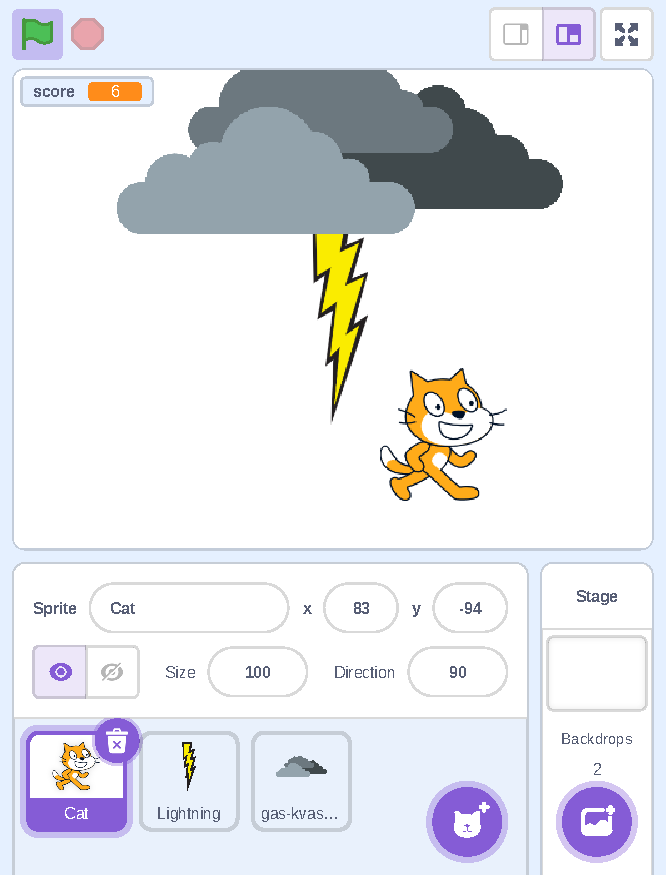
\includegraphics[width=\linewidth]{scratch-execution-model/lightning-game}
            \caption{
                The \textit{Lightning} project in action.
                The user must use the arrow keys to move the cat around, avoiding the lightning bolts.
            }
            \label{fig:the-game-lightning}
        \end{subfigure}
        \begin{subfigure}[T]{0.49\linewidth}
            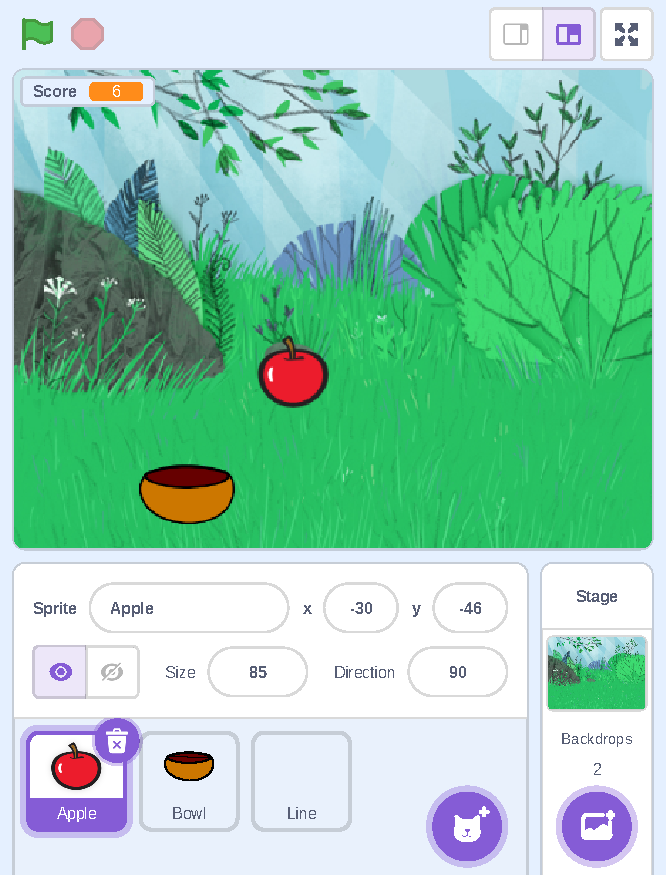
\includegraphics[width=\linewidth]{scratch-execution-model/apple-game}
            \caption{
                The \textit{Catch the apples} project in action.
                The basket follows the mouse, and the user must catch as many apples as possible, without any apples falling on the ground.
            }
            \label{fig:the-game-apple}
        \end{subfigure}
    \end{wide}
    \caption{
        Overview of the two games we discuss.
    }
    \label{fig:the-game}
\end{figure}

\minisec{\textit{Lightning} project}

\begin{figure}
    \begin{subfigure}{\linewidth}
        \centering
        \includestandalone{scratch-execution-model/lightning-scatter-original}
        \caption{
            The original implementation (see bottom left).
            The \textsc{em-30},\textsc{em-60}, and \textsc{em-90} did not achieve 10 points.
        }
        \label{fig:lightning-behaviour-original}
    \end{subfigure}
    \par\medskip
    \begin{subfigure}{\linewidth}
        \centering
        \includestandalone{scratch-execution-model/lightning-scatter-procedure}
        \caption{A modified implementation (see bottom right)}
        \label{fig:lightning-behaviour-procedure}
    \end{subfigure}
    \par\medskip
    \begin{subfigure}{0.49\linewidth}
        \centering
        \begin{scratch}[scale=0.5]
            \blockinit{when \greenflag clicked}
            \blockinfloop{forever}{
                \blockif{if \boolsensing{key \selectmenu{right arrow} pressed?} then}{
                    \blockmove{change x by \ovalnum{10}}
                }
                \blockif{if \boolsensing{key \selectmenu{left arrow} pressed?} then}{
                    \blockmove{change x by \ovalnum{-10}}
                }
                \blockif{if \boolsensing{key \selectmenu{up arrow} pressed?} then}{
                    \blockmove{change y by \ovalnum{10}}
                }
                \blockif{if \boolsensing{key \selectmenu{down arrow} pressed?} then}{
                    \blockmove{change y by \ovalnum{-10}}
                }
            }
        \end{scratch}
        \caption{
            Original implementation of the interactive component.
        }
        \label{fig:the-game-lightning-code-original}
    \end{subfigure}
    \begin{subfigure}{0.49\linewidth}
        \centering
        \begin{scratch}[scale=0.5]
            \blockinit{when \greenflag clicked}
            \blockinfloop{forever}{
                \blockmoreblocks{move}
            }
        \end{scratch}
        \begin{scratch}[scale=0.5]
            \initmoreblocks{define \namemoreblocks{move}}
            \blockif{if \boolsensing{\dots} then}{
                \blockmove{change x by \ovalnum{10}}
            }
            \blockif{if \boolsensing{\dots} then}{
                \blockmove{change x by \ovalnum{-10}}
            }
            \blockif{if \boolsensing{\dots} then}{
                \blockmove{change y by \ovalnum{10}}
            }
            \blockif{if \boolsensing{\dots} then}{
                \blockmove{change y by \ovalnum{-10}}
            }
        \end{scratch}
        \caption{
            Alternative implementation of the interactive component.
            The four if blocks have been moved to a procedure ``run without screen refresh''.
        }
        \label{fig:the-game-lightning-code-better}
    \end{subfigure}
    \caption{
        Behaviour and implementation of the \textit{Lightning} exercise with different execution models.
        In the behaviour (top), marks represent when a new clone is made, while vertical lines indicate when the player either lost (dashed line) or completed 10 points (full line).
        The implementation (bottom) shows both variants of the user interaction code.
    }
    \label{fig:lightning-behaviour}
\end{figure}

The first project we looked at in detail is the \textit{Lightning} project (\cref{fig:the-game-lightning}).\footnote{\url{https://scratch.mit.edu/projects/995927372/}}
The aim of this game is to dodge lightning bolts coming out of the sky.
\Cref{fig:lightning-behaviour-original} gives an overview of the behaviour with the different execution models.
The \textsc{em-30},\textsc{em-60}, and \textsc{em-90} model did not achieve 10 points: they were too slow and made the game unplayable.

This is due to how the interactive component is implemented (\cref{fig:the-game-lightning-code-original}).
Adjusting the implementation by wrapping the user interaction blocks with a procedure (\cref{fig:the-game-lightning-code-better}) enabled solves this issue (\cref{fig:lightning-behaviour-procedure}).
This implementation is usable with all new execution models, except \textsc{em-30}, which remains too slow.

\minisec{\textit{Catch the apples} project}

\begin{figure}
    \centering
    \includestandalone{scratch-execution-model/apple-scatter}
    \caption{
        Behaviour of the \textit{Catch the apples} exercise with different execution models.
        Marks represent score changes (or the initial score at 0), while vertical lines indicate when the player hits 10 points.
    }
    \label{fig:catch-apples-behaviour}
\end{figure}

The second project is the \textit{Catch the apples} project (\cref{fig:the-game-apple}).\footnote{\url{https://scratch.mit.edu/projects/995778768/}}
The aim here is to use the mouse to move a basket and catch as many falling apples as possible.
\Cref{fig:catch-apples-behaviour} shows the behaviour with different execution models.
In this exercise, all models are playable, with \textsc{em-30} behaving the most similar to the original Scratch execution model.
Models faster than \textsc{em-60} are likely too fast to actually play.

\subsection{Discussion}\label{subsec:discussion}

A few conclusions can be drawn from the results of this preliminary benchmark.

First, it is not obviously clear which variation of the execution model is the best universal replacement.
Different types of projects have different needs.
One solution for this problem would be to modify the virtual machine to change the frames per second depending on the type of project that is executed.

Secondly, projects depend on specific behaviour of the virtual machine.
For example, the \textit{Lightning} project's implementation of user interaction only works because of how the current execution model works.
While maybe unfortunate, as there are alternatives that do not depend on this behaviour, this is a consequence of \textit{Hyrum's Law}, which states that ``With a sufficient number of users, [\dots] all observable behaviours of your system will be depended on by somebody''.
Users, however, are already accustomed to changing the duration of wait blocks (and other such blocks) to account for the performance of the Scratch virtual machine on their device.
While not ideal, small differences may thus be acceptable.

Lastly, this illustrates the need for more research into automated evaluation of the behaviour exhibited by Scratch projects.
Some areas of interest are determining what constitutes observable behaviour and when changes to the behaviour become adverse changes.
For example, if projects are executed a bit faster or slower, this might not affect the project's usability.
The existing virtual machine is also not deterministic and depends on system performance: some projects might execute a lot slower on slower hardware, while still being usable.

\section{Impact and conclusion}\label{sec:conclusion}

In \cref{ch:blink}, we proposed a debugger for Scratch with a non-traditional step method.
Instead of stepping a single block at a time, we want to step a single block in every thread of a Scratch program (thus in every script).
However, this introduces two downsides:
\begin{enumerate*}[label=\emph{\roman*})]
    \item the step function exposes internal program state that is normally not visible to the users, and
    \item the debugger uses a different execution model compared to regular execution, whereas a debugger should deviate from normal execution as little as possible
\end{enumerate*}.

This chapter then asks if we can modify the execution model of Scratch in such a way that the step functionality of a debugger is possible and that the changed execution model is usable for normal execution.
To this end, we first took a detailed look at the existing execution model, due to a lack of existing literature on the topic.
This model is the result of multiple years of work in the Scratch virtual machine and contains many nuances.
The current execution model has been chosen to avoid some race conditions but does not avoid all concurrency-related issues: there are some surprising consequences of the threading model in particular.

Any changes to the execution model must not have adverse consequences for existing Scratch projects.
Therefore, we first analyse how Scratch is used by replicating select metrics of previous investigations into what Scratch projects look like.
The most significant previous result in this area is \textcite{aivaloglouHowKidsCode2016}, which analyses Scratch 2.0 projects.
Our results for Scratch 3.0 projects are broadly similar: most Scratch projects are small and simple, but there are a few big and complex ones.

Our proposed changes to the execution model change the threading from cooperative to preemptive.
This implies that more race conditions, which the original execution model sought to prevent, are now possible.
\Textcite{maloneyScratchProgrammingLanguage2010} use the classic example of reading the value of a variable, increasing this value, and finally updating the variable with the new value.
When running the same code unchanged in the new execution model, more race conditions are possible.
However, we believe this is not a big problem, due to two reasons.
First, the kind of code where these race conditions can occur is used infrequently in Scratch.

Second, there is a workaround: the part of the code that must be protected against these race conditions can be extracted into a procedure, using the option ``run without screen refresh''.
This causes the code in the function to become atomic: it will be run without interruptions.
Using this technique is our recommendation for implementing critical sections.
Note that using these critical sections with blocks that require a redraw should be done thoughtfully, as the redraw will not occur (this behaves identically in the current execution model).

Finally, we performed a preliminary benchmark using our proposed changes on a selection of projects, informed by our previous analysis.
The results of the benchmark make clear that finding a single replacement execution model without affecting existing projects is highly unlikely.
Projects depend on the behaviour of the current execution model, meaning any change in behaviour will be a breaking change.
Considering the Scratch Team's (understandable) reluctance to introduce behavioural changes to Scratch at this point, we do not envision our changes being upstreamed, nor would we recommend it, \marginnote{Scratch 4.0?} unless as a breaking change.

While a universally applicable replacement execution model is not achievable, our proposed changes are still useful.
For small projects, the impact of the changes is acceptable, and most projects are small.
Additionally, the new execution model is more suitable for use with our stepping method for debuggers.
We thus envision the new execution model to be used in classrooms where the debugger is used as well.

The results of the benchmarks are also a preliminary exploration.
Our proposed changes must still be validated in educational practice and in a classroom setting with actual users of Scratch, in additional to performing expanded automated benchmarks.
Another area of improvement is looking at more projects with user interaction for benchmarking.
One possible route is investigating heuristics to automatically provide suitable user interaction to those projects, making them suitable for automated benchmarking.
Improving the benchmarking allows for a better understanding on the impact of the proposed execution model.

We also see more opportunities for research on the existing and new execution model of Scratch itself.
For example, the current execution model is defined by its source code.
Constructing a formal mode of the execution model would allow formal reasoning and analysis, which might reveal more opportunities for changes.
This might also be beneficial in further analysing the new model's impact on existing Scratch projects.

\dummypart
\chapter{Conclusions and opportunities}\label{ch:conclusions-and-opportunities}

As an answer to the five research questions mentioned in \cref{sec:a-note-on-the-structure-of-this-thesis},
we introduced five educational tools to facilitate programming education:
two for textual programming languages and three for block-based programming languages.
We also propose changes to the Scratch execution model.

We discuss each research question in detail below.

\section{Textual programming languages}\label{sec:for-textual-programming-languages}

\begin{description}
    \item[RQ1] Can we design an educational software testing framework that supports automated assessment across programming languages based on a single test suite?
\end{description}

We can, as we demonstrate by presenting our implementation of such a testing framework: \textbf{TESTed}.
First, we identified input/output testing and unit testing as two opposing strategies commonly used in educational software testing.
Our initial investigation focused on understanding how these approaches affect the supported programming languages within the testing frameworks.
Often, testing frameworks that fall under input/output testing support multiple programming languages, but the quality of the feedback suffers.
On the other hand, frameworks using unit testing have much more fine-grained feedback, but only support a single programming language.

Our aim was to combine the best of both worlds.
To this end, we formulated the requirements for programming-language-agnostic testing frameworks that combine unit testing with support for multiple programming languages.
We then introduced TESTed, and detailed its internal workings.
Finally, we evaluated TESTed in educational practice to verify that it supports our requirements for a programming-language-agnostic testing framework.

We see opportunities for more work on TESTed in the future.
Our goal is to further develop TESTed for authoring different types of programming exercises across programming languages.
TESTed is currently focused mainly on dynamic testing.
A key area of future interest is the implementation of language-agnostic static code analysis capabilities.

\begin{description}
    \item[RQ2] What is the most ergonomic way to author programming exercises with support for automated assessment across programming languages?
\end{description}

We concluded that a domain-specific language, designed specifically for this purpose, is the best approach.
We then introduced our implementation: \textbf{TESTed-DSL}\@.

We again first looked at input/output testing and unit testing as the two opposing strategies.
However, this time, we focused more on the impact of these strategies on the testing process itself.
We considered what can be tested and how, in addition to how and what feedback is generated.
For example, we considered if input/output testing and unit testing each needed a separate domain-specific language, or if we could merge them into one common one (we did merge them).

The conclusion was again that the best of both strategies provides the best experience for educators.
Looking at programming-language-agnostic testing frameworks more broadly, we reported on three benefits for the adoption of such frameworks: \begin{enumerate*}[label=\emph{\roman*})] \item sharing the same declarative structure across programming languages, \item bridging the gap between input/output testing and unit testing, and \item allowing test code to be expressed in a language-agnostic way.\end{enumerate*}

We also see potential for additions to TESTed-DSL in the future.
These include supporting operator overloading, string conversion, comments, indexing sequences, indexing mappings, destructuring, object identity checking, and object equivalence checking.
Native support for pretty printing nested data structures would be another valuable addition, making it easier to detect differences between expected and actual return values.
There are more opportunities still, including data-driven tests (parameterized tests), supporting dynamic generation of test data and boosting the performance of running tests.

\section{Block-based programming languages}\label{sec:for-block-based-programming-languages}

\begin{description}
    \item[RQ3] Can we design an educational software testing framework for the block-based programming language Scratch?
\end{description}

Yes, as shown by our implementation of such a framework: \textbf{Itch}.
We showed that it offers a versatile approach to testing, allowing static testing, emulating user interaction, and performing post-mortem testing.
Tests can range from purely static to purely dynamic, or a hybrid of both.

However, we also reported that while most exercises can be tested, it remains difficult to design Scratch exercises that are both dynamically testable and sufficiently open-ended to align with the game-like and exploratory nature of Scratch.
Static tests, though faster and sometimes easier to write, can potentially constrain creativity and go against the spirit of Scratch.

We also found that educators that are primarily experienced in Scratch might find JavaScript test suites difficult to write.
For this reason, we created and reported on a prototype of a Scratch-based testing framework called \textbf{Poke}.
It allows creating test suites with Scratch, using the blocks and environment Scratch users are familiar with.
While writing the tests is technically feasible, some challenges remain, the main one being the organizational aspects of managing these Scratch tests suites.

\begin{description}
    \item[RQ4] Can we design an (educational) debugger for the block-based programming language Scratch?
\end{description}

Yes: \textbf{Blink} is our time-travelling debugger for Scratch.
Working with Itch in an educational setting made clear that testing frameworks primarily indicate whether a submission is correct or not, but do not directly assist students in finding the root cause of a failed test.

To address this, we developed Blink, a debugger for Scratch.
Debuggers are generally known to be good tools for finding errors in a program, and this is no different in Scratch.
Blink supports pausing execution, stepping through code, breakpoints, and provides time travel capabilities.
We prioritized the user-friendliness of Blink, given Scratch's younger target audience.
Due to the concurrent nature of Scratch, we had to hide a lot of the complexities of concurrent debugging for the user.
Initial feedback from using Blink in a classroom setting has been positive: students find the debugger intuitive and useful, especially the time-travelling capability.

In the future, we envision integrating Itch with Blink.
In an ideal scenario, a failed test from Itch would allow students to directly open a debugging session when the test failed.
Using the time-travelling features of Blink, students can then go back in time until they find the issue.

\begin{description}
    \item[RQ5] What common execution model for running and debugging Scratch code best optimizes both scenarios?
\end{description}

One of the ways we sought to make the debugger more intuitive was to use a non-traditional stepping functionality.
In most debuggers, a step will advance the code one step in a single thread.
However, in Scratch, we wanted the step to advance one step in all threads simultaneously.
The current execution model makes this difficult.

To answer this research question, we first explained in detail how the current execution model behaves.
The current execution model has been chosen to minimize the occurrence of some concurrency-related issues, like certain race conditions, but does not prevent all issues.
The threading model, in particular, causes some surprising behaviour, which is not ideal as Scratch is intended to be intuitive.

Next, we proposed changes to the execution model of Scratch that seek to resolve these issues.
However, the widespread use of Scratch demands that any changes must not adversely affect existing projects.
For this reason, we explored how Scratch is used, the results of which corroborate previous findings: most Scratch projects are small.

We then performed a preliminary benchmark of the new execution model on various representative projects to measure the real-world impact.
The results of this benchmark make clear that our initial goal of finding a replacement execution model that has no effect on existing projects is not attainable.
Projects rely too much on the behaviour of the original execution model: any change to this behaviour will be a breaking change.
However, the benchmark also showed that the effect on smaller projects is acceptable, and most Scratch projects are small.
We thus believe the new execution model to still be useful: not as a general replacement, but for use in specific contexts.
For example, in a classroom setting, we believe using the new execution model improves the experience of using the debugger.

Finally, we believe more research is needed in regard to the execution model of Scratch.
For starters, the execution model is currently defined by its source code, despite some attempts to create a formal model for it.
As an example, constructing full operational semantics for the execution model would allow better formal reasoning and analysis, which might reveal more opportunities for changes.
Secondly, the changes we proposed in this chapter should be validated experimentally in a classroom setting.
This would allow verification if the proposed changes are intuitive.

% Allow a wide bibliography
\clearpage
\storeareas\StandardArea
\addtolength{\marginparwidth}{-1.5cm}
\KOMAoptions{mpinclude=false}
\recalctypearea
\printbibliography[heading=bibintoc]
\clearpage
\StandardArea

\appendix

\chapter{Task description of the VPW}\label{ch:task-description-of-the-flemisch-programming-contest}

{
    \itshape Below is a translated version of the second Scratch exercise from the 2017 edition of the Flemish Programming Contest (\textdutch{Vlaamse Programmeerwedstrijd}, \textsc{VPW}).
}

\fbox{%
    \begin{minipage}{\textwidth}
        \minisec{Problem 02 (10 points)}
        The stage looks like the drawing below.

        
\includegraphics[width=0.5\textwidth]{appendix-vpw/stage-02}

        Write a program that lets the parrot fly from left to right.
        When he touches the edge, he must turn around.
        The program may only start when the parrot is clicked.
        (Tip: use the ``change costume to \dots'' block for flying)
    \end{minipage}
}


\vspace*{1em}
\textit{Below is a possible solution:}

\begin{center}
    \begin{varwidth}{0.6\textwidth}
        \begin{scratch}[scale=0.6]
            \blockinit{when this sprite clicked}
            \blockmove{set rotation style \selectmenu{left-right}}
            \blockinfloop{forever}{
                \blockmove{move \ovalnum{15} steps}
                \blockmove{if on edge, bounce}
            }
        \end{scratch}
    \end{varwidth}%
    \hspace{1em}%
    \begin{varwidth}{0.6\textwidth}
        \begin{scratch}[scale=0.6]
            \blockinit{when this sprite clicked}
            \blockinfloop{forever}{
                \blockevent{wait \ovalnum{0.2} seconds}
                \blocklook{next costume}
            }
        \end{scratch}
    \end{varwidth}
\end{center}

\end{document}
